\documentclass[ number=1
			   ,series=sidl
				,url=http://langsci-press.org/catalog/book/18 
			   ,isbn=978-3-944675-19-0
			   ,output=long   % long|short|inprep              
			   %,blackandwhite
			   %,smallfont
%			   ,draftmode   
			  ]{LSP/langsci}                          
              
\usepackage{LSP/lsp-styles/lsp-gb4e}		% verhindert Komma bei mehrfachen Fußnoten?
\usepackage{LSP/lsp-styles/avm}
\avmfont{\sc} 
\avmvalfont{\it}

\usepackage{german}
\selectlanguage{USenglish}      

\usepackage{graphicx,float,tabularx,curves}
\usepackage{amsmath}
\usepackage{longtable}

\usepackage{epsfig}

\usepackage{array,arydshln}
%http://tex.stackexchange.com/questions/153303/tipa-package-causing-error-in-xelatex-sups-already-defined
\let\sups\relax\usepackage{tipa}


\usepackage{multicol,amssymb,latexsym}
\def\exfont{\normalsize\it}
\let\eachwordone=\it
\renewcommand{\fnexfont}{\footnotesize\it}

\defcitealias{Tucker:1955}{Tucker \& Mpaayei 1955} %changes the the in text citation of that entry to the value given behind
%\bibpunct[:]{(}{)}{,}{,}{}{,}

\newcommand{\nom}{{\sc nom}}
\newcommand{\gen}{{\sc gen}}
\newcommand{\dat}{{\sc dat}}
\newcommand{\acc}{{\sc acc}}
\newcommand{\abs}{{\sc abs}}
\newcommand{\erg}{{\sc erg}}
\newcommand{\instr}{{\sc ins}}
\newcommand{\ines}{{\sc iness}}
\newcommand{\antgen}{{\sc antgen}}
\newcommand{\voc}{{\sc voc}}
\newcommand{\poss}{{\sc poss}}

\newcommand{\fem}{{\sc f}}
\newcommand{\mas}{{\sc m}}
\newcommand{\neu}{{\sc n}}
\newcommand{\pl}{{\sc pl}}
\newcommand{\sg}{{\sc sg}}
\newcommand{\thirdsg}{3{\sc sg}}

\newcommand{\agnm}{{\sc agnm}}
\newcommand{\ali}{{\sc ali}}
\newcommand{\allo}{{\sc allo}}
\newcommand{\am}{{\sc am}}
\newcommand{\antip}{{\sc antip}}
\newcommand{\appl}{{\sc appl}}
\newcommand{\asp}{{\sc asp}}
\newcommand{\att}{{\sc att}}
\newcommand{\augv}{{\sc augv}}
\newcommand{\aux}{{\sc aux}}
\newcommand{\ben}{{\sc ben}}
\newcommand{\bg}{{\sc bg}}
\newcommand{\caus}{{\sc caus}}
\newcommand{\cert}{{\sc cert}}
\newcommand{\clf}{{\sc clf}}
\newcommand{\coll}{{\sc coll}}
\newcommand{\com}{{\sc com}}
\newcommand{\comp}{{\sc comp}}
\newcommand{\compl}{{\sc compl}}
\newcommand{\complx}{{\sc complx}}
\newcommand{\con}{{\sc con}}
\newcommand{\cond}{{\sc cond}}
\newcommand{\conj}{{\sc conj}}
\newcommand{\cop}{{\sc cop}}
\newcommand{\cs}{{\sc cs}}
\newcommand{\cvb}{{\sc cvb}}
\newcommand{\decl}{{\sc decl}}
\newcommand{\defsc}{{\sc def}}
\newcommand{\dem}{{\sc dem}}
\newcommand{\dep}{{\sc dep}}
\newcommand{\deter}{{\sc det}}
\newcommand{\detr}{{\sc detr}}
\newcommand{\dir}{{\sc dir}}
\newcommand{\dist}{{\sc dist}}
\newcommand{\distr}{{\sc distr}}
\newcommand{\dsbj}{{\sc dsbj}}
\newcommand{\dscn}{{\sc dscn}}
\newcommand{\du}{{\sc du}}
\newcommand{\dubt}{{\sc dubt}}
\newcommand{\dur}{{\sc dur}}
\newcommand{\dyn}{{\sc dyn}}
\newcommand{\ego}{{\sc ego}}
\newcommand{\emphat}{{\sc emph}}
\newcommand{\epen}{{\sc epen}}
\newcommand{\excl}{{\sc excl}}
\newcommand{\faff}{{\sc faff}}
\newcommand{\fin}{{\sc fin}}
\newcommand{\foc}{{\sc foc}}
\newcommand{\fut}{{\sc fut}}
\newcommand{\hab}{{\sc hab}}
\newcommand{\Hyp}{{\sc hyp}}
\newcommand{\icml}{{\sc icml}}
\newcommand{\ideoph}{{\sc ideoph}}
\newcommand{\imp}{{\sc imp}}
\newcommand{\incep}{{\sc incep}}
\newcommand{\Incl}{{\sc incl}}
\newcommand{\ind}{{\sc ind}}
\newcommand{\indf}{{\sc indf}}
\newcommand{\Inf}{{\sc inf}}
\newcommand{\intens}{{\sc intens}}
\newcommand{\intr}{{\sc intr}}
\newcommand{\ipfv}{{\sc ipfv}}
\newcommand{\irr}{{\sc irr}}
\newcommand{\lin}{{\sc lin}}
\newcommand{\loc}{{\sc loc}}
\newcommand{\Mid}{{\sc mid}}
\newcommand{\modal}{{\sc modal}}
\newcommand{\mut}{{\sc mut}}
\newcommand{\Non}{{\sc n}}
\newcommand{\NC}{{\sc nc}}
\newcommand{\Neg}{{\sc neg}}
\newcommand{\nmlz}{{\sc nmlz}}
\newcommand{\NR}{{\sc nr}}
\newcommand{\nts}{{\sc nts}}
\newcommand{\obj}{{\sc obj}}
\newcommand{\obl}{{\sc obl}}
\newcommand{\opt}{{\sc opt}}
\newcommand{\partic}{{\sc part}}
\newcommand{\pass}{{\sc pass}}
\newcommand{\persm}{{\sc pm}}
\newcommand{\propnoun}{{\sc pn}}
\newcommand{\polite}{{\sc pol}}
\newcommand{\pronoun}{{\sc pro}}
\newcommand{\pred}{{\sc pred}}
\newcommand{\prep}{{\sc prep}}
\newcommand{\prf}{{\sc prf}}
\newcommand{\prog}{{\sc prog}}
\newcommand{\prs}{{\sc prs}}
\newcommand{\prtv}{{\sc prtv}}
\newcommand{\proh}{{\sc proh}}
\newcommand{\propr}{{\sc propr}}
\newcommand{\prosp}{{\sc prosp}}
\newcommand{\prox}{{\sc prox}}
\newcommand{\pst}{{\sc pst}}
\newcommand{\pstcont}{{\sc pstcont}}
\newcommand{\pstpunc}{{\sc pstpunc}}
\newcommand{\pstrem}{{\sc pstrem}}
\newcommand{\purp}{{\sc purp}}
\newcommand{\punc}{{\sc punc}}
\newcommand{\pfv}{{\sc pfv}}
\newcommand{\pvs}{{\sc pvs}}
\newcommand{\question}{{\sc q}}
\newcommand{\reas}{{\sc reas}}
\newcommand{\rdp}{{\sc rdp}}
\newcommand{\Recip}{{\sc rec}}
\newcommand{\refl}{{\sc refl}}
\newcommand{\relativ}{{\sc rel}}
\newcommand{\result}{{\sc res}}
\newcommand{\rls}{{\sc rls}}
\newcommand{\sbj}{{\sc sbj}}
\newcommand{\semb}{{\sc semb}}
\newcommand{\simult}{{\sc sim}}
\newcommand{\stat}{{\sc stat}}
\newcommand{\ssbj}{{\sc ssbj}}
\newcommand{\them}{{\sc them}}
\newcommand{\tmp}{{\sc tmp}}
\newcommand{\tns}{{\sc tns}}
\newcommand{\topic}{{\sc top}}
\newcommand{\transitiv}{{\sc tr}}
\newcommand{\uop}{{\sc uop}}
\newcommand{\Verb}{{\sc vblz}}
\newcommand{\ventiv}{{\sc ven}}
                                                      
\usepackage{layout}  
\usepackage{lipsum}   

\hyphenation{Mül-ler lan-gu-a-ges no-mi-na-tive ac-cu-sa-tive for-med mark-ed-S con-tras-tive Was-kia Ame-ri-can de-crea-sing ge-schrie-hen ty-po-lo-gy fre-quen-cies Lich-ten-berk Tur-ka-na mark-ing Sa-ha-ran} 
 
\title{\hspace{1mm}A\,typology of marked-S languages}  
%\title{Τέχνη \newlineCover γραμματική}
%\subtitle{2000+ Years of Language Science and no End in Sight}  
\author{Corinna Handschuh}
\dedication{Für Tommeck}

\typesetter{Corinna Handschuh}
\proofreader{Eitan Grossman, Daniel W. Hieber, Aaron Sonnenschein}

\BackTitle{A typology of marked-S languages}

\BackBody{%
Case"=systems all over the world exhibit striking similarities.  In most languages
  intransitive subjects (S) receives less overt marking than one of the two transitive arguments
  (agent"=like A or patient"=like P); the other one of these two arguments is usually encoded by the
  same form as S. In some languages the amount of overt marking is identical between S, A, and
  P. But hardly ever does the S argument receive more overt marking than A or P.  Yet there are some
  languages that do not follow this general pattern.  This book is about those languages that behave
  differently, the marked"=S languages. 


Marked"=S languages are well"=known to be found in East Africa, where they occur in two different
language families, Afro"=Asiatic and Nilo"=Saharan. They can also be found in North"=Western America
and the Pacific region. This book is the first investigation of marked S"=languages that treats the
phenomenon on a global scale.


The study examines the functional distribution of the two main case"=forms, the form used for S
(S"=case) and the case"=form of the transitive argument which receives less marking (the
zero"=case). It offers a very fine"=grained perspective considering a wide range of constructions.
The contexts in which the case"=marking patterns are investigated include nominal, existential and
locational predication, subjects in special discourse function (e.\,g.\ focused constituents),
subjects of passives and dependent clauses, as well as the forms used for addressing someone
(vocative form) and for using a noun in isolation (citation form).


Apart from the functional distribution of case forms, the formal means of marking are also
considered. The main focus is on the synchronic description and comparison of marked"=S languages,
but historical explanations for the unusual case"=marking pattern are also discussed.
}


%\includeonly{AcknowledgmentsSDL,AbbreviationsSDL,introSDL,methodSDL,nompredSDL,exlocSDL,expsSDL,othclSDL,exsynSDL,typolSDL}
%\includeonly{introSDL}
%\includeonly{methodSDL}
%\includeonly{nompredSDL}
%\includeonly{exlocSDL}
%\includeonly{expsSDL}	
%\includeonly{othclSDL}
%\includeonly{exsynSDL}
%\includeonly{typolSDL}
%\includeonly{conclSDL}

\hypersetup{bookmarksopenlevel=0}
  
\begin{document}             
                                    
\maketitle  
 
\frontmatter 

%\chapter*{Preface}

\tableofcontents   

\addchap{Acknowledgments}

%%%%%%%%%%%%%%%%%%%%%%%NEW

This book started out as a PhD dissertation at Universit\"at Leipzig by the same title, which I submitted in December 2010 and successfully defended in July 2011. 
The original dissertation has undergone minor revisions, but its contents have in essence remained the same.

Many people have contributed to the work in its current state, : to all of whom I would like to express my gratitude.
The original research started out as part of the  project `Marked-absolutive and marked-nominative case systems in synchronic and diachronic perspective' of the \textit{Forschergruppe} `Grammatik und Verarbeitung verbaler Argumente' in Leipzig. 
Financial support for my research has been provided by the Deutsche Forschungsgemeinschaft through a grant to this project.
Michael Cysouw\aimention{Cysouw, Michael}, who was the principal investigator of the project, has patiently accompanied the development of the dissertation from the very beginning. 
He has always provided me with much valued feedback on all aspect of my work from methodological discussion to stylistic comments.  
Without his encouragement, this work would probably not have been completed.
The referees for the dissertation were Martin Haspelmath\aimention{Haspelmath, Martin} and Helen de Hoop\aimention{{de Hoop}, Helen}.
Their comments during and after the writing process, respectively, have been much appreciated and greatly improved the final result. 
 
The research for this book work was carried out during the heyday of the Leipzig typology community.
I was lucky to have had the opportunity to conduct my research as a member of the Max Planck Institute for Evolutionary Anthropology's linguistics department.
Its excellent facilities and stimulating research environment have contributed much to the completion of this work. 
Through the \textit{Forschergruppe}, I also had the chance to collaborate with the larger linguistic community both at the University of Leipzig and the Max Planck Institute for Human Cognitive and Brain Science.

During this time, I presented parts of my work at various occasions in the MPI's `work in progress' series, at the meetings and workshops of the \textit{Forschergruppe} and at `Typologiekolloquium' at Universit\"at Leipzig.
Through these and through the regular interaction with the members of the Leipzig linguistic community and the numerous guests over the years, my work has been greatly inspired.
In particular, I would like to mention (in alphabetical order): Balthasar Bickel\aimention{Bickel, Balthasar}, Bernard Comrie\aimention{Comrie, Bernard}, Tom G\"uldemann\aimention{G{\"u}ldemann, Tom}, Andrej Malchukov\aimention{Malchukov, Andrej L.}, Gereon M\"uller, Jochen Trommer, S\o ren Wichmann, and Alena Witzlack-Makarevich\aimention{Witzlack-Makarevich, Alene}, with whom I also taught a course at \emph{Leipzig Springschool on Linguistic Diversity} in 2008. 
The preparations for this course have been very valuable for my research. 
In addition, I would like to thank the following people for providing information on the languages of their expertise:
Lea Brown\aimention{Brown, Lea} on Nias\il{Nias}, Gerrit Dimmendaal\aimention{Dimmendaal, Gerrit} on Turkana\il{Turkana}, and Claudia Wegener\aimention{Wegener, Claudia} on Savosavo\il{Savosavo}.
Another important factor in completing a work of this extent are your fellow sufferers, a.k.a the other PhD students.
For sharing the woes of PhD life, more often a laugh and the occasional drink, I want to thank my peers at the MPI: Joseph Atoyebi, Joseph Farquharson, Diana Forker, Linda Gerlach, Thomas Goldammer, Iren Hartmann, Hagen Jung, Zaira Khalilova, Nina Kottenhagen, Christfried Naumann, Andrey Nefedov, Sven Siegmund, Eugenie Stapert, Matthias Urban, and Jan Wohlgemuth.

I would further like to thank the audiences of my presentations at the following conferences, where parts of this work were presented:
\emph{NAWUKO} 2006 at Konstanz,  \emph{ALT} 2007 at Paris, \emph{Syntax of the World's languages} 2008 at Berlin and \emph{Case in and across languages} 2009 at Helsinki. 
I also would like to thank the organizers of those conferences.

Finally, there are the people who contributed to the publication process of this very book you are holding in your hands (or more likely seeing on your screen). 
I am very glad for the opportunity to publish a revised and updated version of my original thesis as one of the first books of Language Science Press.
I must thank Martin Haspelmath for accepting my book for the series Studies in Diversity Linguistics and thus making my work widely available.
Being one of the first book being published meant witnessing many, and starting some, discussions on formatting.  
Martin Haspelmath and Stefan M\"uller were very helpful in answering my questions on all kinds of issues from alphabetization to the correct usage of hyphenation in large compounds.
Together with Timm Lichte, Stefan M\"uller also reliably and quickly gave feedback on the more technical issues with the \LaTeX -style.  
The tedious work of proof-reading has been done by Eitan Grossman, Daniel W. Hieber and Aaron Huey Sonnenschein. 
All three of them have done an incredible job in a very short time. 
While I was preparing the book for publication, I could rely on the great atmosphere at the linguistics department at Universität Regensburg. 
Special thanks go to my colleagues there, Martine Bruil, Christian Rapold and Zarina Molochieva, for their support in many ways. 

\enlargethispage{\baselineskip}
Needless to say, all shortcomings, omissions and remaining fallacies of this work are my own responsibility.



 


\addchap{List of abbreviations}

\begin{multicols}{2}
\begin{tabbing}
long gloss \= \kill
`X'>`Y' \> X acting on Y\\
1 \> 1{st} person \\
2 \> 2{nd} person \\
3 \> 3{rd} person \\
A \> most agent-like argument\\ \>  of transitive verb\\
%ABL \> ablative case\\
\abs \> absolutive case\\
{\acc} \> accusative case\\
%AFF \> (Havasupai)\\
\agnm \> agent nominalizer\\
%ALL \> allative case\\
\ali{} \> alienable possession\\
\allo{} \> allocentric referent\\
\am{} \> associative marker\\
\antgen \> antigenitive case\\
\antip{} \> antipassive\\
\appl{} \> applicative\\
%ART \> article\\
\asp{} \> aspect marker\\
\att{} \> attributive\\
\augv{} \> augmentative vowel\\
\aux{} \> auxiliary\\
%\ben{} \> benefactive\\
\bg{} \> background\\
CA \> common argument\\
\caus{} \> causative\\
\cert{} \> certainty marker\\
\clf{} \> classifier\\
\coll{} \> collective\\
\com{} \> comitative\\
%\comp{} \> complementizer\\
\compl{} \> completive\\
\complx{} \> complex marker (Gamo)\\
\con{} \> continuous tense (Maasai)\\
\cond{} \> conditional\\
\conj{} \> conjunction\\
\cop{} \> copula\\
\cs{} \> construct state\\
\cvb{} \> converb\\
%\dat{} \> dative case\\
\decl{} \> declarative\\
\defsc{} \> definite\\
\dem{} \> demonstrative\\
\dep{} \> dependent clause\\
\deter{} \> determiner\\
\detr{} \> detransitivizer\\
\dir{} \> directional\\
\dist{} \> distal\\
%\distr{} \> distributive\\
\dsbj{} \> different subject\\
\dscn{} \> discourse connective\\
\du{} \> dual\\
\dubt{} \> dubitative\\
%\dur{} \> durative\\
\dyn{} \> dynamic\\
\ego{} \> egocentric referent\\
\emphat{} \> emphatic\\
\epen{} \> epenthetic segment\\
\erg{} \> ergative case\\
\excl{} \> exclusive\\
\fem{} \> feminine\\
\faff \> final affix\\
\fin{} \> finite\\
\foc{} \> focus\\
\fut{} \> future\\
\gen{} \> genitive case\\
\hab{} \> habituative\\
\Hyp{} \> hypothetical\\
\icml{} \> incompletive aspect\\
\ideoph{} \> ideophone\\
\imp{} \> imperative\\
%\Incl{} \> inclusive\\
\incep{} \> inceptive\\
\ind{} \> indicative\\
%\indf{} \> indefinite\\
\ines{} \> inessive\\
\Inf{} \> infinitive\\
\instr{} \> instumental\\
\intens{} \> intensifier\\
\intr{} \> intransitive\\
\ipfv{} \> imperfective\\
\irr{} \> irrealis\\
LDG \> Lexical Decomposition\\
\> Grammar\\
\lin{} \> linker clitic (Boraana\\ \> Oromo)\\
\loc{} \> locative case\\
\mas{} \> masculine\\
MDS \> multidimensional scaling\\
\Mid{} \> middle, mediopassive\\
\modal{} \> modal verb\\
\mut{} \> mutated form (Nias)\\
\neu{} \> neuter\\
\Non{}\_`X' \> non-`X'\\
\NC{} \> noun class marker\\
\Neg{} \> negation, negative\\
\nmlz{} \> nominalizer\\
\nom \> nominative case\\
NP \> noun phrase\\
\NR{} \> nominal realis\\
\nts{} \> non-topical subject\\
O \> $\equiv$ P\\
\obj{} \> object\\
\obl{} \> oblique\\
\opt{} \> optative\\
OT \> Optimality Theory\\
P \> most patient-like argu- \\ \>  ment of transitive verb \\
\partic{} \> particle\\
\pass{} \> passive\\
p.c. \> personal communication\\
\pfv{} \> perfective\\
\pl{} \> plural \\
\persm{} \> person marking\\
\propnoun{} \> proper noun\\
\polite{} \> polite form\\
\poss{} \> possessive\\
\pronoun{} \> pronoun \\
\pred{} \> predicative\\
\prep{} \> preposition\\
\prf{} \> perfect\\
\prs{} \> present tense\\
\prtv{} \> partitive case\\
\prog{} \> progressive\\
%\proh{} \> prohibitive\\
\propr{} \> proprietive\\
\prosp{} \> prospective\\
\prox{} \> proximal/proximate\\
\pst{} \> past tense\\
\pstcont{} \> past continuous\\
\pstpunc{} \> past punctual\\
\pstrem{} \> remote past \\
\purp{} \> purposive\\
\punc{} \> punctual\\
\pvs{} \> preverbal selector (Arbore)\\
\question{} \> question particle/marker\\
%QUOT \> quotative\\
\reas{} \> reason\\
\rdp{} \> reduplication\\
\Recip{} \> recipient\\
%RECP \> reciprocal\\
\refl{} \> reflexive\\
\relativ{} \> relative clause\\
\result{} \> resultative\\
\rls{} \> realis\\
S \> single argument of in-\\ \>  transitive verb\\
\sbj{} \> subject\\
%SBJV \> subjunctive\\
%\semb{} \> semblative\\
\sg{} \> singular\\ 
\simult{} \> simultaneous\\
\stat{} \> stative\\
\ssbj{} \> same subject\\
\them{} \> thematic suffix (Nandi)\\
\tmp{} \> temporal\\
\tns{} \> tense marker\\
\topic{} \> topic\\
\transitiv{} \> transitive\\
\uop{} \> unspecific object (Wappo) \\
\Verb{} \> verbalizer\\
\ventiv{} \> ventive extension\\
\voc{} \> vocative
\end{tabbing}
\end{multicols}

\mainmatter

\part{Preliminaries}

\chapter{Introduction}\label{introduction}

%%%%%%%%%%%%%%%%%%%%%%%%%%
%%%%%% SECTION 1.1 %%%%%%%
%%%%%%%%%%%%%%%%%%%%%%%%%%

\section{Marked"=S coding}\label{coding}\is{alignment|(}

Syntactic typology traditionally distinguishes languages by the way they encode the single argument of an intransitive verb (S) compared to the more agent-like (A) and the more patient-like arguments (P) of a monotransitive verb \citep{Comrie:1978,Dixon:1979,Dixon:2010-1}. 
On this basis, the two main alignment types, namely \textsc{nominative"=accusative} and \textsc{ergative"=absolutive} (Figure~\ref{Alignment}), are dis\-tin\-guish\-ed. 
While\is{alignment!through case-marking|(}  the nominative"=accusative\is{alignment!nominative-accusative|(} pattern employs the same form for S and A (nominative case\is{case!individual forms!nominative}), the P argument receives a special form of encoding (so-called accusative\is{case!individual forms!accusative} case)\is{alignment!nominative-accusative|)}.  
In an ergative"=absolutive\is{alignment!ergative-absolutive|(} system,  S and P are coded alike (absolutive\is{case!individual forms!absolutive} case) while the A argument is in a special form (ergative\is{case!individual forms!ergative} case)\is{alignment!ergative-absolutive|)}.

\begin{figure}[ht] \centering \fbox{
\begin{picture}(265,95)
\put(10,75){\makebox(100,15)[l]{nominative"=accusative:}}

\put(45,45){\makebox(20,20){\textbf{S}}}
\put(15,15){\makebox(20,20){\textbf{A}}}
\put(75,15){\makebox(20,20){\textbf{P}}}

\put(85,25){\circle{20}}
 
\closecurve(40,60, 65,65, 60,40, 40,20, 15,15, 20,40)

\put(150,75){\makebox(100,15)[l]{ergative"=absolutive:}}

\put(185,45){\makebox(20,20){\textbf{S}}}
\put(155,15){\makebox(20,20){\textbf{A}}}
\put(215,15){\makebox(20,20){\textbf{P}}}

\put(165,25){\circle{20}}
 
\closecurve(190,40, 185,65, 210,60, 230,40, 235,15, 210,20)
\end{picture}}

\caption{Nominative"=accusative vs. ergative"=absolutive alignment}\label{Alignment} \end{figure}\is{alignment|)}\is{alignment!through case-marking|)} 

In\is{marked-S languages!formal definition|(} most languages, overt formal marking is employed for the P argument in nominative"=accusative\is{alignment!nominative-accusative} languages and the A argument in ergative"=absolutive\is{alignment!ergative-absolutive} languages, while the relation including the S argument (i.e. S+A for the former and S+P for the latter type) is typically left zero-coded\is{markedness!overt versus zero-coding}.\footnote{The label `unmarked' is often used for the case-form lacking overt morphological marking. 
However, this terminology is problematic because the term `unmarked' is used for a variety of concepts in linguistics \citep{Haspelmath.mark:2006}. 
I follow Haspelmath's proposal to use the term `zero-coded' for the formal manifestation of unmarkedness.}  
This tendency was prominently phrased in \citeauthor{Greenberg:1963}'s Universal 38:

\begin{quote} Where there is a case system, the only case which ever has only zero allomorphs is the one which includes among its meanings that of subject of the intransitive verb.
\citep[75]{Greenberg:1963}
\end{quote}  

However, there are clear exceptions to this generalization. 
I will use the term \textsc{marked"=S language} in the following to refer to those exceptional languages. 
More precisely, there are two types of marked"=S languages: \textsc{marked"=nominative} and \textsc{marked-absolutive}. 
Both have in common the property that the single argument of intransitive verbs is overtly-coded while one of the transitive arguments (A or P) receives zero-coding.\footnote{No examples are known to me of a language using zero-coding for both A and P but overt coding for the S argument -- a pattern which would by my definition be included in the group of marked"=S languages. 
Given the overall rarity of horizontal alignment (i.e. in which A and P are treated alike but differently from S) and the rarity of marked"=S systems, it does not come as a surprise that the combination of both rarities is not (yet) found.} 
%\textcolor{red}{Koenig:2008 p.9 refers to Donohue & Brown 1999 and Plank's Rarit\"atenkabinet for the claim that Chukchi absolutive singular nouns (encoding S) are the morphologicaly most complex, I have not found this citation yet, still needs to be checked}
This study presents an in-depth survey of marked"=S languages.\is{marked-S languages!formal definition|)}

I will begin this first chapter by defining marked"=S languages, which constitute a rare and somewhat unexpected type of encoding grammatical relations (Section~\ref{definition}). 
Following this introduction, a brief digression will be made to discuss the phenomenon known as grammatical markedness and the different usages of the term (Section~\ref{markedness}). 
Then I will address the issue of terminology used in describing the case-forms of a nominal in a language of the marked"=S type. 
Since a wide range of different case-terms\is{caseterminology} are used in the descriptions of marked"=S languages. 
In order to assure consistency within this work, I will employ a uniform set of case-terms. 
In addition, I will propose a new terminology to be employed when comparing\is{case!comparative concepts} marked"=S languages with each other (Section~\ref{label}). 
Following that, I will discuss the explanations and types of explanations given to justify the existence of this rare type of case-system (Section~\ref{explain}). 
These explanations will be grouped into two types: historical and functional explanations.
The subsequent section discusses marked"=S systems from the point of view of formal linguistic theories. 
Not only do marked"=S languages constitute a typological exception, they also pose a serious problem for various formal theories of case-marking, as will be demonstrated using the example of Lexical Decomposition Grammar (Section~\ref{theoretical}).
Alignment is most prominently associated with nominal case-marking, and this study is likewise restricted to marked"=S alignment as it is found in this domain. 
However, the term `alignment' is also used to refer to verbal agreement and word order, as well as with reference to behavioral properties of nominals. 
Marked"=S coding in those other domains, or the domain-specific counterparts thereof, will briefly
be discussed in Section~\ref{domains}.\enlargethispage{\baselineskip}
Finally, I will give an outline of the remainder of this study in Section~\ref{outline}.

%%%%%%%%%%%%%%%%%%%%%%%%%%%%%%%%%%%
%%%%%%%%%% SECTION 1.2 %%%%%%%%%%%%
%%%%%%%%%%%%%%%%%%%%%%%%%%%%%%%%%%%

\section{Definition}\label{definition}

Marked"=S languages are more traditionally known by the name \textsc{marked"=nominative} languages\is{alignment!marked-nominative}. 
I have chosen this new term in order to allow the inclusion of data from a related, yet not so widely recognized, phenomenon, namely \textsc{marked"=absolutive} languages. 
The term \textit{marked"=S} also nicely summarizes the central characteristic of this type of language, namely the overt marking found on the single argument of intransitive verbs (S) combined with a zero-coded A or P argument. 

The marked"=nominative\is{alignment!marked-nominative|(}  type is the most frequent manifestation of the marked"=S coding type. 
As a subtype of the nominative"=accusative alignment system, marked"=nominative languages exhibit the basic pattern exemplified for this system in Figure~\ref{Alignment}. 
In marked"=nominative systems -- like in standard nominative"=accusative -- S is aligned with A and opposed to P. 
Unlike in the standard system, the P relation is left without any formal encoding of its case relation. 
It is in the zero-coded form, while the S+A relation (the nominative) has an overt morphological marker (cf. Figure~\ref{MN alignment}). 
In contrast, the standard -- `unmarked' -- nominative"=accusative system uses overt marking either for both S+A (nominative) and P (accusative) or restricts it to P-marking. 

\begin{figure}[htbp]\centering\fbox{
\begin{picture}(225,70)
%\put(10,72){\makebox(90,15)[l]{Marked nominative:}}

\put(95,40){\makebox(20,20){\textbf{S}}}
\put(65,10){\makebox(20,20){\textbf{A}}}
\put(125,10){\makebox(20,20){\textbf{P}}}
 
\closecurve(90,55, 115,60, 110,35, 90,15, 65,10, 70,35)

\put(3,30){\makebox(65,15){overt coding}}
\put(65,37){\vector(1,0){25}}

\put(150,30){\makebox(55,15){zero-coding}}
\put(168,33){\vector(-2,-1){28}}

\end{picture}}
\caption{Marked"=nominative coding}\label{MN alignment}
\end{figure}

The two types of coding are illustrated here by some examples.
The Turkish\il{Turkish} data in (\ref{Turkish}) exemplify the standard nominative"=accusative system with a zero-coded Nominative\footnote{Throughout the text, I follow the convention of capitalizing case-labels, when referring to a specific case-form in an individual language.}  case and an overtly coded Accusative\is{case!individual forms!accusative} case-marked by the suffix \emph{-\i}. 
\enlargethispage{2\baselineskip}

\begin{exe}\ex\label{Turkish}\langinfo{Turkish}{Altaic; Turkey}{own knowledge}
\begin{xlist}
\ex\label{TurkishS}\gll Adam gel-di\\
man.{\nom{}} come-\pst{}\\
\glt `The man came.'
\ex\label{TurkishAP}\gll Ö\v{g}retmen adam-\textbf{\i}{} gör-dü\\
teacher man-\acc{} see-\pst{}\\
\glt `The teacher saw the man.'
\end{xlist}
\end{exe}

The marked"=nominative type is illustrated by examples from Cocopa\il{Cocopa}. 
The S and A relation in (\ref{Cocopa}a, b) is marked with the overt Nominative suffix \emph{-c} while the P relation in (\ref{CocopaAP}) is left zero-coded.

\begin{exe}\ex\label{Cocopa}\langinfo{Cocopa}{Yuman, Hokan; Mexico}{\citealp[183, 186]{Crawford:1966}}
\begin{xlist}
\ex\label{CocopaS}\gll\textipa{ap\'a\textbf{-c}} \textipa{aw-y\'a}\\
man-{\nom{}} 3-know\\
`The man knows.'
\ex\label{CocopaAP}\gll \textipa{ap\'a\textbf{-c}} \textipa{k\super{w}\'ak} \textipa{pa:-\textsubdot{t}\'Im}\\
man-{\nom{}} deer.{\acc{}} 3>3-shoot\\
`The man shot the deer.'
\end{xlist}
\end{exe}\is{alignment!marked-nominative|)} 

\is{alignment!marked-absolutive|(}A parallel system to the marked"=nominative type exists for ergative"=absolutive languages -- the marked"=absolutive type. 
Again, the marking relations are reversed from the standard type. 
The standard ergative"=absolutive system overtly codes the A relation (ergative\is{case!individual forms!ergative}) and leaves the S+P relation (absolutive\is{case!individual forms!absolutive}) zero-coded. 
Conversely, in marked-absolutive languages one finds overtly coded S+P and zero-coded A. The marked-absolutive system is illustrated in Figure~\ref{MA-align}. 
Just like the marked"=nominative, the marked-absolutive contradicts Greenberg's universal quoted above since it has overt marking of the S argument while zero-coding one of the transitive core relations. 

\begin{figure}[ht]
\centering
\fbox{
\begin{picture}(225,70)
%\put(10,72){\makebox(90,15)[l]{Marked absolutive:}}

\put(95,40){\makebox(20,20){\textbf{S}}}
\put(65,10){\makebox(20,20){\textbf{A}}}
\put(125,10){\makebox(20,20){\textbf{P}}}
 
\closecurve(100,35, 95,60, 120,55, 140,35, 145,10, 120,15)

\put(3,35){\makebox(65,15){zero-coding}}
\put(53,38){\vector(1,-1){17}}

\put(153,27){\makebox(55,15){overt coding}}
\put(150,35){\vector(-1,0){30}}
\end{picture}}
\caption{Marked"=absolutive coding}\label{MA-align}
\end{figure}

To illustrate the two patterns, I provide examples for ergative"=absolutive and marked-absolutive coding below.
In Chechen\il{Chechen}, the S and P relation is zero coded (\ref{Chechen}a, b, c) while the A relation in (\ref{Chechen}b, c) is overtly coded by the Ergative\is{case!individual forms!ergative} suffix \emph{-(a)s}.
In addition to the ergative"=absolutive case-marking, verbal indexing\is{verbal indexing} also has an ergative"=absolutive basis. 
The verb agrees in gender with the S and P argument. 

\pagebreak
\begin{exe}\ex\label{Chechen}\langinfo{Chechen}{Nakh-Daghestanian; Chechen Republic}{Zarina Molochieva, p.c.}
\begin{xlist}\ex\label{ChechenS}\gll naana baazar j-ax-na\\
mother(\fem{}) market.ADV \fem{}-go-\prf{}\\
\glt `The mother went to the market.'

\ex\gll k'ant-\textbf{as} naana lie-j-i-na\\
boy(\mas{})-{\erg{}} mother(\fem{}) lie-\fem{}-make-\prf{}\\
\glt `The boy has lied to the mother.'

\ex\gll naana-\textbf{s} k'ant liicna-v-i-na\\
mother(\fem{})-{\erg{}} boy(\mas{}) wash-\mas{}-make-\prf{}\\
\glt `The mother has bathed the boy.'
\end{xlist}
  \end{exe}

The only known straightforward example of a marked"=absolutive case-system so far is attested in Nias\il{Nias}.\footnote{\citet{Crysmann:2009}, using a quite different definition of marked"=absolutive language, argues against classifying Nias\il{Nias} as such. 
In his approach, alignment is not considered to be construction specific as it is in my account and many other recent works that study alignment from a cross-linguistic perspective \citep[cf. among others][]{Bickel.align}. 
I will discuss this the notion in more detail in Section~\ref{domains} and Chapter~\ref{method}.} 
While the S argument in (\ref{NiasS}) is in the overtly marked Absolutive\is{case!individual forms!absolutive} case, the A argument is in the zero-coded Ergative\is{case!individual forms!ergative} form of a noun (\ref{NiasAP}). 
As illustrated in (\ref{NiasP}), the P relation is also encoded in the overtly coded Absolutive\is{case!individual forms!absolutive} form.\footnote{The distinction between the Absolutive and Ergative case-form is not always as straightforward as in example (\ref{Nias}a, c). 
In most cases the difference is marked by initial consonant mutation, see Section~\ref{morphophon} for a brief discussion of the morphophonemics of nominal mutation\is{case-marking!via nominal mutation} in Nias\il{Nias}.}
  
\begin{exe}\ex\label{Nias}\langinfo{Nias}{Sundic, Western Malayo Polynesian, Austronesian; Sumatra, Indonesia}{\citealp[343]{Brown:2001}, Lea Brown, unpublished fieldwork data from 2003,  \citealp[346]{Brown:2001}}
\begin{xlist} 
\ex\label{NiasS}\gll aukhu \textbf{n-}idan\"o\\
{\stat}.hot {\abs}-water\\
\glt `The water is hot.'
\ex\label{NiasAP}\gll i-f-o-houu	defao 	\textbf{idan\"o} 	nasi\\
3\sg{}-\caus{}-have-rust	iron.\abs{}	water.\erg{}	sea.\abs{}\\
\glt `The seawater rusted the iron'
\ex\label{NiasP}\gll  la-bunu \textbf{m-}ba\ss i\\
3\pl{}.{\rls}-kill \abs{}-pig\\
\glt `They killed a pig.'
\end{xlist}
\end{exe}
\is{alignment!marked-absolutive|)}

In\is{marked-S languages!functional definition|(} addition to this definition of marked"=S coding, which is purely based on the absence versus presence of overt case-marking\is{marked-S languages!formal definition}, there is a second definition of marked"=S languages. \citet{Koenig:2006} distinguishes between Type 1 and Type 2 marked"=nominative languages. 
Type 1 languages are classified by the criterion I have discussed above, namely the overt coding of the nominative case-form and the zero-coding of the accusative\is{case!individual forms!accusative}. 
Type 2 languages have overtly coded case-forms for both nominative and accusative. 
However, the accusative\is{case!individual forms!accusative} has a wider range of functions; it is for example the form of a noun used in citation. 
I will discuss this second definition of marked"=S coding in Section~\ref{functional}.\is{marked-S languages!functional definition|)}

%%%%%%%%%%%%%%%%%%%%%%%%%%
%%%%%% SECTION 1.3 %%%%%%%
%%%%%%%%%%%%%%%%%%%%%%%%%%

\section{Markedness in grammar}\label{markedness}\is{markedness|(}

The term \textit{markedness}, and more often the statement that a certain linguistic feature is \textit{marked}, are often employed in grammatical descriptions.
Markedness, in its most basic meaning, is universally associated with the presence of overt material, such as overt case morphology for example. 
Other aspects that are often also called \textit{markedness} frequently correlate with formal markedness (i.e. the presence of overt material). 
These other factors include (often interrelated) phenomena such as restriction in use, late and/or cumbersome acquisition of a structure, specialization in meaning, or a low usage frequency of an item. 
Even if not correlated with formal markedness in any sense, structures that meet any of these additional criteria may be referred to as marked by many linguists. 
\citet{Haspelmath.mark:2006} discusses the different meanings of the term markedness and distinguishes between twelve basic senses. 
These twelve senses are roughly grouped into four types that view markedness as either complexity, difficulty, abnormality or a multidimensional correlation. 

The notion of markedness has a prominent position in both functionally- and formally-oriented linguistic traditions. 
In the functional tradition, this notion goes back to the work of Roman Jakobson\aimention{Jakobson, Roman} and other members of the Prague School, while in the formal tradition the notion was made prominent by Noam Chomsky\aimention{Chomsky, Noam}.
In both cases the concept of markedness appears to have been inspired by phonological work.
\citet{Battistella:1996} provides a detailed discussion of the understanding and evolution of the term markedness in the Jakobsoninan and Chomskyan traditions. 

With respect to marked"=S languages, the term \textit{marked} is principally understood as overt coding. 
As mentioned at the end of the previous section, an extension of the term marked to other criteria can also be seen for marked"=nominative languages, namely in the definition of Type 2 marked"=nominative languages proposed by \citet{Koenig:2006}. 
In the following, I will attempt to make clear which one of the different definitions of markedness is presently being discussed.
When referring to the form-based definition of markedness, I will use the terms \textsc{overtly coded} or respectively \textsc{zero-coded}. 
Only when directly quoting the work of other authors, the terms `markedness', `marked' and  unmarked' may be used for describing forms that differ in term of more versus less overt material (i.e. the form based criterion)\is{markedness|)}. 


%%%%%%%%%%%%%%%%%%%%%%%%%%%%%%%%%%
%%%%%%%%%% SECTION 1.4%%%%%%%%%%%%
%%%%%%%%%%%%%%%%%%%%%%%%%%%%%%%%%%

\section{Case-labels}\label{label}\is{case!terminology|(}

When describing the case-system of a given language, linguists often apply traditional case-terminology familiar from Latin. 
If a case does not resemble any case in the Latin case-system, linguistic theory today provides a huge arsenal of Latinate case-labels to be employed \citep[cf.][]{Haspelmath:2009}. 
This practice of reusing terms is not uncontroversial, since the range of functions or meanings of case-forms will virtually never coincide between any two languages. 
Marked"=S languages are a prime example of this variation of functions. 
Their nominative/absolutive and ergative/accusative forms show properties quite unlike the properties of case-forms that are known by the same name in standard nominative"=accusative or ergative"=absolutive languages.
This has led many scholars working on marked"=S languages to abandon the traditional labels.
Yet many of the alternate labels they came up with are equally inappropriate. 
In this section, I will discuss the different approaches for labeling cases in marked"=S languages.
Furthermore, I will introduce the case-terminology to be employed in the remainder of this book.

As described in the definition of marked"=S coding above (Section~\ref{definition}), the special property of the marked"=S system is that it combines the standard alignment of nominative"=accusative or ergative"=absolutive languages with an unexpected pattern of overt/ non-overt marking of the nominal cases. 
The decision between choosing a label according to the function of a form or according to the overt marking relations is also the main problem when it comes to finding appropriate names for the individual cases defining this alignment system. 
   
One possibility is to simply use the labels from the standard nominative"=accusative and ergative"=absolutive systems.
So\is{case!individual forms!nominative|(}, the term `nominative' is used for the S+A relation in standard nominative"=accusative as well as in marked"=nominative systems. 
Similarly, the label `absolutive\is{case!individual forms!absolutive}' refers to the S+P relation in standard ergative"=absolutive and in marked-absolutive systems. 
However, the more problematic issue is how to label the zero-coded case in the marked"=S systems.  
Not only do the terms `accusative\is{case!individual forms!accusative}' and `ergative\is{case!individual forms!ergative}' suggest overt marking of the case relation \citep[56--57]{Dixon:1994}, the uses of the zero-coded case-forms also go beyond those of the accusative or ergative as found in the standard versions of these alignment systems. 
Nonetheless the  label `accusative\is{case!individual forms!accusative}' is used in the description of a number of marked"=nominative languages, namely Maa\il{Maa} \citepalias{Tucker:1955}, Murle\il{Murle} \citep{Arensen:1982} and K'abeena\il{K'abeena} \citep[85--86]{Crass:2005}. 
The labels of `nominative' and `accusative\is{case!individual forms!accusative}' are also employed by \citet{Koenig:2006,Koenig:2008} in her overview of marked"=nominative languages in Africa.

Differently, \citet{Dixon:1979} proposed the term `extended ergative' for the marked nominative case to reflect its overt marking, which is parallel to the mostly overtly marked ergative\is{case!individual forms!ergative} in ergative"=absolutive systems. 
The label `extended accusative' for the marked-absolutive would be analogous to this label, though he does not propose this term since he disputes the existence of marked-absolutive systems altogether. 
The `extended ergative', however, did not make it into the terminology of grammar writers.\footnote{In theoretical typology, the term has done a little better. 
\citet{Plank:1985} uses the terms `extended ergative/restricted absolutive' to refer to the marked"=nominative system and also `extended accusative/restricted nominative' for the marked absolutive pattern.} 
If discussed at all, it is merely mentioned as a possible alternative label, for example by \citet[133]{Wegener:2008}, who irrespective of this calls the Savosavo\il{Savosavo} subject-marker `Nominative'. 
Dixon appears to have had a change of mind on the appropriate terminology for marked"=nominative systems, as he concludes in his \citeyear{Dixon:1994} work that ``it seems wisest to maintain the standard use of ergative to refer to marking just of A function'' \citep[64]{Dixon:1994} and proposes to stick to the term marked"=nominative after all.  

One strategy that avoids the terminological problem altogether is not to use any of the traditional Latinate case names at all. 
Most often this results in labels such as `subject-case' and `object-case' (or just `subject-marker'). 
This approach is chosen by the grammar writers of some African languages, e.g. for Borana Oromo \citep[34]{Stroomer:1995} or Gamo\il{Gamo} \citep[364]{Hompo:1990}. 
Most commonly it has been applied to languages of the North-American West-Coast -- especially in the 60s and 70s of the last century. 
This is the case for the Yuman languages Cocopa\il{Cocopa} \citep[104]{Crawford:1966}, Diegue\~no\il{Diegue\~no (Mesa Grande)} \citep[151]{Langdon:1970}, Mojave\il{Mojave} \citep[18]{Munro:1976}, Yavapai\il{Yavapai} \citep[68]{Kendall:1976} and Hualapai \citep[38]{Watahomigie:2001}. 
The same is true for the non-related language Wappo\il{Wappo} \citep*[90]{Lietal:1977}. 
However, in their grammar of Wappo\il{Wappo} -- published about thirty years later -- the same authors have switched from the term `subject-marker' to the use of \textit{nominative} \citep*{Thompsonetal:2006}. 
The labels `subject-case' and `object-case' have the disadvantage that they carry theoretical connotations unrelated to marked"=S case-marking. 
Not all nouns bearing the overt marking of subjects might be subjects in a syntactic sense, and not all syntactic subjects might have the subject case-marker in a certain language (unless one establishes overt case-marking as the only defining property of subjects in that language). 

Drawing very much on the Latin grammar tradition, \citet{Melcuk:1997} makes an idiosyncratic proposal for labeling compared to the current practice in descriptive linguistics. 
For Maa\il{Maa}, he suggests to stick to the literal translation of the term `nominative' as `the naming case' and therefore proposes to use it for the form used in naming a nominal (i.e. the citation form\is{citation form}). 
Apart from the use as citation form, this case also encodes the P argument of a transitive verb (`Accusative'\is{case!individual forms!accusative} case in other descriptions of Maa\il{Maa}). 
The subject-marking case he relabels as `Oblique' in turn. 
This usage of the term Nominative may be well motivated from a historical and etymological perspective as \citet[453]{Creissels:2009} points out. 
Still, if used for the case-form encoding transitive objects, the term Nominative is bound to give rise to confusion. 
Beyond being extremely confusing, there is -- in my opinion -- a major problem with this approach, % to take the literal translation of the case name as the basis for picking the case-form to stick the lable nominative on. 
namely, that the etymological meaning is not the meaning most prominently associated with the nominative. 
It is rather its function as the `subject-case' that comes to mind first, maybe along with the function as `default' or `elsewhere' case for some linguists.\footnote{The notion of default case is discussed in more detail in Section~\ref{theoretical}.} 
Both functions are fulfilled by \citeauthor{Melcuk:1997}'s `Oblique' case and not his `Nominative'.
%\citet{Creissels:2009} makes a similar proposal to the labeling of cases

The terminologies traditionally employed for the marked"=nominative languages of Eastern Africa are far less confusing. 
`Nominative' is used in the traditional way as referring to the S+A relation.\is{case!individual forms!nominative|)} 
To\is{case!individual forms!absolute|(} account for the special status of the form used for the P relation, this form is not referred to as `accusative\is{case!individual forms!accusative}' but as the `absolute' case -- e.g. in Turkana\il{Turkana} \citep{Dimmendaal:1982} or Datooga\il{Datooga} \citep{Kiessling:2007}. 
The same terminology of `Absolute' and `Nominative' case was also introduced in an early description of the Yuman language Yuma \citep[210]{HalpernYuma3}, although it did not catch on in the terminology of this genus, as noted above. 
Also \citet[456]{Creissels:2009} proposes `absolute' as a label for nouns in extra-syntactic function such as citation forms, which tend to be zero-coded morphologically (all these function are covered by the typical East-African absolute).
Some linguists also use the term `absolutive' (rather than absolute). 
This is attested, for example, in the description of Harar\il{Oromo (Harar)} Oromo by \citet{Owens:1985}. 
This, however, might lead to confusion with the S+P relation in ergative"=absolutive languages. 
Therefore absolute should be preferred as a label. 
Finally, \citet[24]{Koenig:2008}, in her discussion of the marked"=nominative case-terminology, notes that the term `absolute' might also lead to confusion since it is used for the zero-coded Nominative\is{case!individual forms!nominative} case-form in Turkish\il{Turkish}. 
This leads her to use the term `accusative\is{case!individual forms!accusative}' also for marked"=nominative languages.\is{case!individual forms!absolute|)} 

Given all these different traditions and approaches to naming cases in marked"=S languages, one is bound to get mixed up in the terminology when comparing data from different languages. 
In order to spare the reader from confusion by changing glosses from one example to the next, I decided not to stick to the case-labels chosen by the linguists working on the individual languages. 
Instead, I will change the glosses with the goal of achieving maximum transparency. 
All examples from marked"=nominative languages are uniformly named and glossed as \textsc{nominative}\is{case!individual forms!nominative} and \textsc{accusative}\is{case!individual forms!accusative}. 
I have chosen this convention for the following reasons.
There seems to be a certain trend towards recognizing the overt subject-marker as parallel to the nominative case-marker in any standard nominative"=accusative language. 
This trend is indicated by \citeauthor{Thompsonetal:2006}'s (\citeyear{Thompsonetal:2006}) change of terminology as well as Dixon's change of mind concerning the `extended ergative' vs. `marked"=nominative' terminology. 
Moreover, this proposal involves the least amount of relabeling of case-forms and thus makes going back to the original sources less prone to requiring terminological adjustments. 

`Accusative\is{case!individual forms!accusative}' and `absolute\is{case!individual forms!absolute}' both appear to be good choices for the non-no\-mi\-na\-tive case in marked"=S languages. 
The encoding of transitive P arguments is just one of many functions the zero-coded case-form fulfills in marked"=nominative languages, as I will demonstrate in the following (Chapters~\ref{nompred}--\ref{extrasyn}). 
The label `accusative\is{case!individual forms!accusative}' is traditionally associated with a case-form with the main function of encoding P arguments. 
Using this label for a case-form that has a variety of additional functions may lead to mild confusion on the first encounter with examples in which the accusative argument is clearly not an object\is{grammatical relation!object} of any kind. 
This study aims at exploring the functions of the different case-forms in marked"=S languages, and thus wants to draw attention of those functions of the object-case in marked"=nominative languages that are unusual compared with standard nominative"=accusative languages. 
In contrast, the label `absolute' is less familiar and might be mixed up with `absolutive' and thus lead to the wrong impression that one is dealing with an ergative"=absolutive language. 
In the remainder of this study I will use the term `accusative\is{case!individual forms!accusative}' to refer to the case-form that (among other functions) encodes transitive P arguments in marked"=nominative languages. First, I do so because of the greater familiarity of the term `accusative' over `absolute'. 
Also, as noted above, the range of uses of the object case-form in marked"=nominative languages is a central aspect of this study. 
Therefore, unexpected occurrences of accusative\is{case!individual forms!accusative} case, from the standpoint of the more widely known standard nominative"=accusative system, are meant to be highlighted here.

For the marked"=absolutive system, we are not confronted with such hard decisions about terminology, since one is not faced with any differing traditions of labeling. 
\citet{Brown:2001} uses the terms \textsc{Unmutated} and \textsc{Mutated} form of the noun for Nias\il{Nias}. 
These labels refer to the morphophonemic shape of the nouns in question. 
The Mutated form covers the absolutive\is{case!individual forms!absolutive} (i.e. S+P) function, while the Unmutated form is used for A arguments among others. 
Since Nias\il{Nias} is the only language with a marked-absolutive system in my study, I will adopt the language-specific terms Mutated and Unmutated form referring to the S+P relation (the absolutive\is{case!individual forms!absolutive}) and A relation (the ergative\is{case!individual forms!ergative}), respectively. 

The previous discussion has dealt with the issue of labeling cases in individual languages.
In addition, terminology is needed to make general statements about the overtly coded and zero-coded forms in both marked"=nominative and marked-absolutive languages. 
For this purpose I propose the following terminology, which will be employed throughout the study whenever making comparative statements.  
When referring to marked"=S languages I use the terms \textsc{S-case}\is{case!comparative concepts!S-case} and \textsc{zero-case}\is{case!comparative concepts!zero-case} form. 
The label S-case refers to the case which includes among its functions that of encoding the single argument of an intransitive verb (overtly coded in all languages under investigation by definition). 
This is the nominative (S+A) in marked"=nominative languages and the absolutive\is{case!individual forms!absolutive} (S+P) in Nias\il{Nias}. 
The zero-case on the other hand refers to the P argument in marked"=nominative languages and the A argument in marked-absolutive languages. 
This case-form is expressed by zero-morphology in the overwhelming majority of marked"=S languages.\is{case!terminology|)}  
%I could have used these terms on all levels of description (the language level, and the intermediate levels generalizing over a subtype of marked"=S language). However, for the benefit of readability I stick to the more common and transparent terms. 
      
%The marked nominative and marked absolutive types of language pose a problem to the descriptive linguist, when it comes to assigning a label to a case. Aside of being the case associated with S+A marking (or the `subject' case) the term nominative  has some additional connotations. Taking literally, the Latin Nominative is the `naming case', and does hence imply the use as a citation form. Also the nominative is considered the `default' or `elsewhere' case by many theories, which implies a wide range of uses.  


%%%%%%%%%%%%%%%%%%%%%%%%%%
%%%%%% SECTION 1.5 %%%%%%%
%%%%%%%%%%%%%%%%%%%%%%%%%%


\section[Explaining the existence of marked"=S]{Explaining the existence of marked"=S}\label{explain}

\subsection{Rare and geographically skewed}
Languages of the marked"=S type are a typological exception. 
Their occurrence is unexpected, a view expressed for example by Greenberg's (1963) Universal 38 cited above. Not surprisingly, languages of this type are extremely rare and their occurrence is geographically highly skewed. 
The main locus for marked"=S languages is in North-Eastern Africa \citep[138]{Koenig:2008}. 
Apart from the cluster in Africa, the pattern is also found in the Yuman genus of southwestern North America and a few other languages of that region, as well as in some languages of the Pacific region. 

To account for the existence of this unexpected case-system, two types of explanations have been put forward, a historical one and a functional one. 
The historical explanation describes how the marked"=S system can evolve from one of the more widespread systems. 
This explanation has been put forward for languages of the marked"=nominative type, and considers them to be an extended variant of ergative"=absolutive systems with overtly coded ergative case-marking, which has been extended to cover the S relation. 
Apart from ergative"=absolutive systems a variety of other sources have been suggested for marked"=nominative languages. 
What all of these historical scenarios have in common is that they propose an origin for the nominative from a category which is expected to be overtly coded from a cross-linguistic perspective.  
The second type of explanation draws on the number of other functions the case-forms in the marked"=S system cover beyond S, A and P marking. 
This theory predicts that the overall distribution of the zero-coded form will be broader than the distribution of the overtly coded form if one takes into consideration other functions, such as marking of attributive possessors, marking of predicate nominals etc.
Of course, these two types of explanations are more different points of view than mutually exclusive approaches.\footnote{I have to thank Eitan Grossman for reminding me of this.} 
Historical change in a language can certainly be explained by functional motivations in many cases.
Some scholars would even argue that functional motivations are the ultimate explanation for all language change \citep{Keller:1994,Dubois:1987,Croft:2000}.

While both types of explanations try to account for the fact that marked"=S languages occur in the first place, the two approaches fall short of explaining the rarity of the phenomenon.
In this section, the two lines of argumentation will be discussed in more detail starting with the historical explanation in Section~\ref{historical}, followed by the functional motivation in Section~\ref{functional}.  


\subsection{Historical explanations}\label{historical}\is{marked-S languages!historical explanations|(}

A prominent advocate of the historical explanation of marked"=S systems is \citet{Dixon:1979,Dixon:1994}.
He defines marked"=nominative languages purely on the basis of the contrast between overt and zero-coding \citep[76ff.]{Dixon:1994}. 
Yet, he also tries to give an explanation for the existence of these typologically rare languages.
Dixon\is{grammatical relations!subject|(} argues that marked"=nominative languages exist because ergative"=absolutive languages constitute a somewhat unsatisfactory case-system in neglecting the `universal concept' of subject and might eventually amend for this by extending the use of A-marking to S.

\begin{quote} The extension of `marked A case' can be explained in terms of the universal syntactic-semantic identification of A and S as `subject'
\citep[78]{Dixon:1979} \end{quote} 

Along\is{alignment!marked-absolutive|(} the same line of argumentation, Dixon denies the existence of marked"=absolutive languages.
Since, according to him, nominative"=accusative languages are more well-formed in this respect, there is no need for overt P-marking to extend its use to mark S.
There is thus no reason why marked-absolutive languages should emerge in the first place.\is{grammatical relations!subject|)}

\begin{quote} 
There is a more slender semantic link between O  and S, so that the fourth logical possibility---`marked O case' being extended to also cover S---appears not to occur.\footnote{Dixon's `O' corresponds to `P' in the terminology used here.} \citep[78]{Dixon:1979}  \end{quote}\is{alignment!marked-absolutive|)}

An ergative\is{case!individual forms!ergative} origin of the marked"=nominative coding-system has also been suspected by linguists confronted with individual languages of this type. 
\citet{Lietal:1977} analyze the Wappo\il{Wappo} marked"=nominative system as a recent innovation. 
They vaguely hint that the overt subject-marker might be a trace of an earlier ergative stage ``where the absolutive case was unmarked and the modern Wappo\il{Wappo} \emph{-i} was the ergative case-marker that became generalized into a subject-marker'' \citep[98]{Lietal:1977}. 
However, they elaborate an alternative pathway for the means of encoding grammatical relations in modern Wappo\il{Wappo}, which might be in conflict with the hypothetical ergative\is{case!individual forms!ergative} in pre-modern Wappo\il{Wappo}. 
Their main argument for the innovative status of the Wappo\il{Wappo} marked"=nominative is its absence from subordinate clauses and equational sentences. 
Both sentence types have a rigid SOV word order, while main clauses (of the non-equational type) are more flexible in the ordering of constituents. 
Since ``subordinate clauses are known to be more conservative than main clauses in preserving'' word order -- citing \citet{Lehmann:1974} and \citet{Vennemann:1975} on this -- they conclude that Wappo\il{Wappo} must be moving from a stage where grammatical relations were encoded by word order to a stage where this is done via case-marking \citep[100]{Lietal:1977}. 
So basically they propose a change from word order to case-marking, on the one hand, and a change within the case-marking system (namely from ergative"=absolutive to marked"=nominative), on the other hand. 
Of course, it would be possible that the two events took place sequentially. 
First, the word order-based system changed to an ergative case-marking system with a freer word order, which then in turn became a marked"=nominative system. 
Yet this is a highly speculative proposal, which cannot be backed up by any historical records of the language. 
The first records on the Wappo\il{Wappo} language date back to the early twentieth century and at this time the marked"=nominative system was already established, as the first grammar by \citet[131]{Radin:1929} shows. 
Since doubt is cast on the classification of Wappo\il{Wappo} being closely-related to the Yukian languages by \citet{Sawyer:1980}, a comparison with these languages to reconstruct earlier stages of Wappo\il{Wappo} will most likely not help in solving the riddle of the origins of the Wappo\il{Wappo} marked"=S system. 

The former-ergative analysis is the most widespread line of historical explanation for marked"=nominative languages, yet there are a number of other explanations that have been suggested in the literature. 
An overview of various possible historical scenarios for the rise of overt-nominative marking is provided by \citet[178]{Koenig:2008}.  
She proposes for example a passive agent marker as another possible source for an overt nominative marker. She suggests that Maa\il{Maa} could be a case of this scenario. 
This pro\-po\-sal is parallel to what has been suggested as the origin of ergative\is{case!individual forms!ergative} markers for many languages. \citet{Anderson:1977} lists Polynesian languages such as Tongan, Niuean and Samoan, Australian languages, such as Walpiri, as well as Indo-European languages of the Indic and Iranian subgroups, for which a passive origin of ergativity has been proposed.  
The parallel scenario has not been widely discussed for marked"=nominative languages so far -- not to mention the doubts which have been cast on this origin for ergative languages (cf. for example Hindi as discussed by \citealp{ButtKing:2004}).

While the theories mentioned so far all search for the origin of the marked"=nominative within a prior stage of the case-system, there are other hypotheses suggesting that overt nominative-marking might have originated from a different domain of grammar altogether. 
The first such proposal sees the nominative marker as a reanalyzed definiteness marker, while another suggest an origin as a topic-marker. 
The definiteness origin is proposed for the Northern Lwoo languages Anywa, P\"ari\il{P\"ari}, and Jur-Luwo by \citet[179]{Koenig:2008}. 
Note also that \citet{Reh:1996} still analyzes the form under discussion in Anywa as a definite subject and does not consider the system a fully-fledged case-system. 
An origin as a topic-marker is suggested for the marked"=nominative of East Cushitic by \citet{Tosco:1994}. 
He lists two reasons for this assumption. 
First, subject-marking  only occurs with definite subjects in some of the East Cushitic languages, a feature he associates with topicality. 
Secondly, Tosco notes that nominative case-marking is not found with focused subjects in many of the languages under investigation. 

One critical point that has been ignored by all proponents of the historical explanations of marked"=S alignment is the immense rarity of this system. 
In other words, if there are so many routes that lead to marked"=S alignment, why are there so few marked"=S languages around?
This point is especially problematic for the `extended ergative' theory put forward by \citet{Dixon:1994}, since this approach states a universal pressure for ergative"=absolutive languages to become marked"=nominative -- yet standard ergative"=absolutive languages are far more numerous than marked"=nominative languages.
\citet[312--313]{Maslova:2000} suggests two reasons why a linguistic structure might be rare on a worldwide scale. 
One reason is that something is rare because there are hardly any ways in which a given linguistic structure can arise -- a situation that does not seem to hold for marked"=S coding given all the historical scenarios discussed above.  
The other possible reason for cross-linguistic rarity is that even though a linguistic structure may arise through a number of pathways, there are still more pathways leading away from that structure. 
So once a system has come into existence, it will very quickly be lost because it changes into yet another structure.

One example for such a rise and quick demise of marked"=S alignment is Old French\il{French (Old)}. 
While the old Latin case-system was abandoned, traces of the Latin Nominative remained, which were in fact the only traces of overt nominal inflection on full NPs. 
Therefore nouns distinguish only two case-forms (\ref{OldFre}), the Nominative form  that is encoded with the suffix \emph{-s} in most cases and the zero-coded Oblique form comprising all non-subject functions \citep[182]{Detges:2009,Jespersen:1992}.

\begin{exe} \ex\label{OldFre}\langinfo{Old French}{}{\citealp[94]{Detges:2009}}
\begin{xlist}
\ex\label{OldFreNom}\gll li chien-s mort l' ome\\
\deter{}.\sbj{} dog-\nom{} bites \deter{}.\obl{} man.\obl{} \\
\glt `The dog bites the man.'
\ex\label{OldFreObl}\gll le chien mort li uem\\
\deter{}.\obl{} dog.\obl{} bites \deter{}.\nom{} man.\nom{}\\
\glt `It is the dog whom the man bites.'
\end{xlist}
\end{exe}

In contemporary French\il{French}, the Nominative endings have been eliminated, making the marked"=nominative stage a transitional episode during the transfer from case-marking to positional licensing of grammatical relations. 
Notably, this quick episode of the marked"=S coding-system in French did not come about by any of the historical sources proposed in the literature, but simply by morphophonological attrition.  
However, not all marked"=S systems appear to be this short-lived. 
Since this alignment system spreads over major branches of language families, as in, e.g. Cushitic or the Yuman languages, marked"=S appears to be a rather stable system in these genealogical groupings.\is{marked-S languages!historical explanations|)}

\subsection{Functional explanations}\label{functional}\is{marked-S languages!functional definition|(} 

The second proposal to account for the existence of marked"=S systems is based on the range of functions individual case-forms have in a language.
This approach reduces the impact of the formal marking of case-forms. As a consequence, a different sense of the term markedness is employed for marked"=S languages by \citet{Koenig:2006,Koenig:2008}. 
She distinguishes between what she calls Type 1 and Type 2 marked"=nominative languages. 
Type 1 languages overtly code the S+A relation, while using a zero-coded form for P. 
Type 2 languages on the other hand employ overtly coded forms for all core relations, but the form employed for P is functionally unmarked (i.e. it covers the wider range of functions). 
I will refer to the two types as formally (Type 1) and functionally (Type 2) marked"=S languages.

The formal and functional criteria for identifying marked"=S languages coincide in the majority of cases. 
In other words, most languages which overtly code the S-case will employ the zero-case in a wider range of functions than the S-case. 
And vice versa, the case which covers the widest range of functions in a language will typically receive the least amount of overt coding. 
However, there are some exceptions to both generalizations. 
As this study will show, the overtly marked S-case sometimes covers all the functions one would expect of a non-marked nominative -- Maidu\il{Maidu} \citep{Shipley:1964} is a prime example of this. 
And conversely, even if a non-S-case has a wider range of functions, it will not necessarily receive less overt marking than the S-case -- this situation is found  for example in Wolaytta\il{Wolaytta} \citep{Lamberti:1997} or Gamo\il{Gamo} \citep{Hompo:1990}. 

The\is{marked-S languages!formal definition|(} formal approach is the more traditional way of characterizing marked"=S systems and is based on the presence or absence of overt formal marking of the different case relations. 
One short-coming of this approach is that it exclusively focuses on the encoding of the S, A and P arguments. Other functions the case-forms might have in the language under investigation are neglected. 
Those other functions are, for example, the usage to mark attributive possessors, predicate nominals or subjects of passive clauses. 
These other functions are taken into consideration in the second approach of defining marked"=S systems -- the functional one. 
This approach takes other functions besides S, A and P marking into account when identifying which case is the marked one and which is the default case\is{case!default}. 
This definition coincides with a slightly different notion of marked"=S languages in which overt marking of the S relation and zero-coding of one transitive relation is not a prerequisite.\is{marked-S languages!formal definition|)} 
The functional definition of marked"=S languages also includes languages in which all of the core verbal arguments (S, A, and P) are equally marked in terms of overt morphology, but the form used for the grammatical relation including S is used in less functions than the case-form used for the other core argument (P with nominative"=accusative and A with ergative"=absolutive alignment). 

The functional view of marked"=S alignment is advocated by \citet{Koenig:2006}. 
It is also the predominant take on this system by most scholars working on the marked"=S languages of Eastern Africa -- although it is usually not explicitly phra\-sed. 
The special role attributed to the zero-coded form in these languages is for example mirrored in the label chosen for this case-form, i.e. `absolute' or `absolutive\is{case!individual forms!absolutive}', which recognizes its wider use than just encoding the P relation (cf. Section~\ref{label}).  

This functional approach is put to the test within this study by examining the range of functions the different case-forms cover within marked"=S languages. 
In her formulation of the functional approach K\"onig states quite openly that the accusative\is{case!individual forms!accusative} is ``used with the widest range of functions'' (\citeyear[138]{Koenig:2008}). 
However, she does not explicitly define how this widest range of functions is to be measured. 
It appears that she is counting the number of different functions a certain case-form has, without distinguishing how peripheral or central to the grammar a certain function is. 
Also, she does not clearly explain how she arrives at the list of functions she is using in her comparison.  
One could, for example, argue that subjects of mono- and ditransitive verbs constitute two separate functions.\footnote{\citet[403]{Bickel.align} discusses a language encoding the two functions in distinct ways, namely Gyarong\il{Gyarong} (Sino-Tibetan).}
Furthermore, certain verb classes\is{verb class} are known to employ non-standard case-forms for their subjects in many languages, e.g. so-called experiencer-subjects. 
Marking the subject arguments of these verb classes could arguably be seen as separate functions.
As a result, the number of function an individual case-form has will vary considerably for the same language depending on the initial set of functions one considers.

\is{marked-S languages!functional definition!strong versus weak hypothesis|(}Irrespective of this, there are two possible interpretations of the claim of functional markedness of the S-case in marked"=S languages, and correspondingly two hypotheses one could test. 
In what I call the \textsc{weak version} of the functional markedness hypothesis, the widest range of functions is simply measured by comparing the range of functions of the zero-case with the range of functions of the S-case in a given language. 
In the \textsc{strong version} of the hypothesis the range of functions of the zero-case is not only measured against the number of functions of the S-case, but also against the combined number of functions of every other case-form in the language. 
Of course, for languages with a two term case-system both hypotheses make the same predictions. 
However, as \citet{Koenig:2008} notes, quite a number of the marked"=S languages of Africa have a larger inventory of case-forms. 
Also the marked"=S languages of North-America have somewhat more complex case-systems.
In this study I will test both versions of the functional markedness hypothesis -- the weak one and
the strong one.\is{marked-S languages!functional definition!strong versus weak hypothesis|)}%
%\enlargethispage{\baselineskip}

Like the historical explanations of marked"=S coding, the functional approach does not directly address the cross-linguistic rarity of this alignment system.
However, there is a promising line of argumentation for the dispreference of marked"=S alignment within this approach.
In what \citet[91--93]{Mallinson:1981} label the `discriminatory theories' of case, one would expect that the S argument -- which does not need to be distinguished from any other argument -- will be encoded with the zero-coded case-form. 
Therefore the same form will be employed for any transitive argument aligning with S.
%one step missing here, probably frequncy of zero-form (therefor other functions)
Using overt morphology on the S argument -- though there is no need for discriminating it from some other argument and thus no need for overt marking -- is a dispreferred strategy and therefore should not be widely distributed among the world's languages.
For similar reasons a number of other functions of a noun will be encoded with the zero-coded form. 
When using a noun in the citation\is{citation form} form (or other isolated context), there is no need for distinguishing its argument role from some other argument. 

In addition to providing the more promising explanation for the rarity of mark\-ed"=S languages, the functional approach also scores better in explaining marked"=absolutive\is{alignment!marked-absolutive} languages. While for the historical approaches integration of the marked"=absolutive system into the explanation is either doubtful or excluded by definition -- as it is the case for the `extended ergative' theory -- no such restriction exists for the functional approach. 
The zero-case is the one with the widest range of functions and whether the S-case comprises an S+A or S+P relation is irrelevant.\is{marked-S languages!functional definition|)} 
          
%In marked"=nominative languages the nominative case has some special properties as compared to the accusative. In the formal -- more traditional -- approach this special property of the nominative is its overt morphophonemic marking, while the accusative case has no such marking. In the functional approach to marked nominative languages this special property of nominative case is its restricted use, whereas the accusative has the property of a default case which is used in a wide variety of constructions

%%%%%%%%%%%%%%%%%%%%%%%%%%
%%%%%% SECTION 1.6 %%%%%%%
%%%%%%%%%%%%%%%%%%%%%%%%%%

\section{Implications for formal approaches to case-marking}\label{theoretical}

As noted in Section~\ref{definition}, the unexpectedness of the marked"=S system has been expressed by \citet{Greenberg:1963}, based on cross-linguistic observations.
The general tendency for the nominative\is{case!individual forms!nominative} and absolutive\is{case!individual forms!absolutive} to be encoded with less overt material has also been acknowledged by some formal linguists.
The following quote by \citet{Chomsky:1993} expresses the same observation as Greenberg's generalization (and extends it to the domain of verbal agreement).\enlargethispage{2\baselineskip}
  
\begin{quote}
The `active' element (Agr$_{S}$ in nominative"=accusative languages and Agr$_{O}$ in ergative"=absolutive languages) typically assigns a less-marked Case to its Spec, which is higher on the extractability hierarchy, among other properties. It is natural to expect less-marked Case to be compensated (again, as a tendency) by more-marked agreement (richer overt agreement with nominative and absolutive than with accusative and ergative). 
\citep[10]{Chomsky:1993}
\end{quote}

Beyond this brief statement, marked"=S languages are of no further relevance for Chomsky's theory, which when it comes to case is mostly concerned with the underlying deep-structure relations. 
Not much room is dedicated to the actual surface case-forms which are generated in spell-out. 
However, there are other formally-oriented linguistic paradigms for which marked"=S languages are of great relevance, since their existence poses a great challenge to the mechanisms of case-assignment underlying these theories.

Already in early work on case-systems, the nominative had a special status among the case-forms of the paradigm. 
This observation was often expressed by noting that, strictly speaking, only nouns in the nominative case can be viewed as nouns, while all other forms were just `cases of a noun', i.e. they were not considered to be nouns themselves. 
\citet[24]{Sweet:1876} for instance held the view that all ``oblique cases are really attribute-words.''
Likewise, in modern linguistics a strict division is  often made between the nominative and all other cases. 
As a result of this, some scholars treat the nominative (at least if zero-coded) as an non-case altogether, as exemplified in the following quotation; similar formulations can be found in \citet{Aissen:1999,Aissen:2003} and \citet[566]{deHoop:2008}:
 
\begin{quote}
We assume that nominative (or absolutive) case is in fact a label for `no case': that is, we assume that the absence of special morphological marking indicates the absence of case. 
\citep[322]{deHoop:2005}
\end{quote}

Even without denying case status to it, the special status of the nominative case is undisputed by theories of case. 
This special status is often referred to as it being the {`default'} or {`elsewhere'} case\is{case!default}. 
The elsewhere case is not restricted in its usage by any conditions on its occurrence, unlike, for example, German\il{German} Dative subjects, which have to be licensed by certain mental state verbs.
Because of its principally unrestricted usability, the nominative is the case that occurs in the widest range of functions, which is exactly the property ascribed to the zero-accusative by the functional approach to marked"=nominative languages. 
As a consequence, some theories run into trouble when confronted with marked"=S languages, since the default\is{case!default} case nature of the nominative is hard-wired into their structure. 

In some theories, the default\is{case!default} status of the nominative is not only an underlying assumption, but is actually built into the theory via a set of features or some similar technical apparatus.
The cases within the paradigm are specified with respect to those abstract features. 
Notably, the default\is{case!default} case is then analyzed as the maximally underspecified case (i.e. the set of features characterizing it is the empty set).
Hence there are no restrictions on the occurrence of the default\is{case!default} case, which means it could theoretically occur in all contexts.
The default\is{case!default} case is, however, subject to the Elsewhere Principle\is{Elsewhere Principle} \citep{Kiparsky:1973}.
Thus if a given contexts meets the feature specification of another case-form, this more specific case-form will be picked over the default\is{case!default} case.
 
As\is{Lexical Decomposition Grammar|(} an example I will discuss Lexical Decomposition Grammar (henceforward LDG) in some detail and the difficulties arising due to the existence of marked"=S languages. 
LDG \citep{Wunderlich:1997,Stiebels:2002} assigns the following underspecified feature to the grammatical core cases:

\begin{itemize}
\item Dative: [+hr,+lr] 
\item Ergative: [+lr] 
\item Accusative: [+hr] 
\item Nominative/Absolutive  : [\quad]
\end{itemize}

Arguments are assigned case according to their theta-structure.
The feature [+hr] translates to `there is a higher role', which means in order for an argument to be assigned a case with this feature, there must be another argument that has a higher role. 
Conversely, the [+lr] feature requires an argument bearing a lower role necessary.
The lexical entry of a verb can override the features specified in theta-structure \citep{WunderlichLakaemper:2001}; however, for the moment we will neglect this. 
The following example illustrates the case-assignment in LDG.  In (\ref{LDGSF}) the theta-structure and semantic form of the verb `to see' are given.
The lambda abstractors in the theta-structure generalize over the argument variables of the verb -- {s} being the situation (or event) variable, which is not relevant for the argument structure -- increasing from left to right with respect to how deeply they are embedded into the semantic form of the verb.
For each argument (i.e. {x} and {y} in example (\ref{LDGSF})), there is a higher role if another argument is embedded less deeply into the semantic form. 
Conversely, if there is an argument that is embedded more deeply, a lower role exists.
 
\begin{exe}
\ex\label{LDGSF}
$ \underbrace{ \lambda x \quad \lambda y \quad \lambda s}_{\text{\normalsize\rm theta-structure}}$
\qquad $ \underbrace{\{ \text{see} (x,y)\} (s)}_{\text{\normalsize\rm semantic form}} $ 
\end{exe}

The argument positions in theta-structure are fully specified with respect to their [hr] and [lr] features, thus they can be assigned both positive or negative values for the respective features. 
Example (\ref{LDGTS}) demonstrates the mechanism of case-assignment to the arguments of a verb. 
In this process, a language assigns the case-forms  which are at disposal in its lexical case inventory to these fully specified argument positions. 
Contradictions between the feature specifications of argument position and case-marker are not tolerated by the mechanism. 
For a position for which the language finds no better matching feature specification in its case inventory, the maximally underspecified default\is{case!default} case will be picked. 
Nominative"=accusative languages assign accusative\is{case!individual forms!accusative} case to the {y} arguments since its specification as [+hr] fits into this argument slot. 
For the {x} argument no case with matching features is found. 
Hence, the default\is{case!default} nominative case is assigned. 
Conversely, ergative"=absolutive languages have a matching candidate for the [+lr] feature of the {x} arguments -- the ergative\is{case!individual forms!ergative} case -- but no other candidate than the default\is{case!default} case for the {y} argument.  

\begin{exe}
\ex\label{LDGTS}
\begin{tabbing}
nominative"=accusative \quad \= \nom{} \quad \= \kill
{} \> $\lambda x$\>$\lambda y$\\
{}\> -hr\>{+hr} \\
{}\> {+lr}\>-lr \\
nominative"=accusative\> \nom{} \>\acc{}	\\
ergative"=absolutive\> \erg{} \>\abs{} 
\end{tabbing}
\end{exe}

While the LDG approach neatly derives the case-assignment in standard no\-mi\-na\-tive-accusative and ergative"=absolutive languages, the system is not as suitable for marked"=S languages. 
The default\is{case!default} case is best described, not by the case functions it covers, but by stating that it is used in all contexts in which all other cases cannot be used. 
For the standard systems, this property is reflected in the LDG feature specification.  
In marked"=S languages, the role of a default\is{case!default} case must be ascribed to the zero-case, since this is the case with the elsewhere distribution. 
Thus, the feature-values LDG proposes for accusative and ergative case do not do justice to zero-accusatives or zero-ergatives found in marked"=S languages. 
Furthermore, if one adopts the LDG case feature specifications, one  would have to assume a correspondence between zero-exponence (no overt morphology) and non-zero feature sets for the zero-accusative [+hr] or zero-ergative [+lr]. 
And conversely, one would postulate a relation between overt exponence and zero-feature specification for the marked"=nominative or marked"=absolutive.  
That leaves one with a `NO form to meaning' relationship on the one hand and a `form to NO meaning' relationship on the other hand.
This is a most unsatisfying situation, which violates basic principles of morphological theory.\is{Lexical Decomposition Grammar|)} 
In the concluding part of this work, I will come back to this issue (Section~\ref{consequencesformal}). 
For now, I just note that in addition to being typologically rare, marked"=S languages do not seem to fit into the patterns that a number of formal theories offer for analyzing case-assignment.

%%%%%%%%%%%%%%%%%%%%%%%%%%%%%%%%%%%%%%%%%%%
%%%%%%%%%%%%%% SECTION 1.7 %%%%%%%%%%%%%%%%
%%%%%%%%%%%%%%%%%%%%%%%%%%%%%%%%%%%%%%%%%%%

\section{Domains of alignment}\label{domains}

\subsection{Beyond case-marking}\is{case-marking}
The discussion of marked"=S languages so far has exclusively focused on nominal case-marking\is{alignment!through case-marking}.
The labels \textit{nominative"=accusative} and \textit{ergative"=absolutive} are commonly employed to classify the system of case-marking on the noun phrase (i.e. de\-pen\-dent-marking). 
However, the terms are also applied more generally for any morphosyntactic device treating S like A or P, and thus including verbal indexing\is{alignment!through verbal indexing}\is{verbal indexing} (i.e. head-marking). 
In some instances, the terminology has even been expanded to word order\is{alignment!through word order} \citep{Buth:1981, Andersen:1988}. %
In addition, behavioral properties have been used to characterize the alignment system(s) of a languages \citep{Bickel.align}, thereby extending the term alignment beyond coding-properties.

I will discuss these other domains of alignment -- head-marking (Section~\ref{head}), word order (Section~\ref{order}) and behavioral properties (Section~\ref{behavior}) -- and clarify for all of these domains what the marked"=S equivalent would look like. 
All of these domains have some limitation with respect to the possibility of investigating the marked"=S system in them. 
For nominal case-marking, some restrictions exist as well. 
In the final section (Section~\ref{invest}), I will state these limitations and thus define the exact domain of this study on marked"=S languages, namely, nominal case-marking of full noun phrases.

\subsection{Head-marking}\label{head}\is{alignment!through verbal indexing|(}\is{verbal indexing|(}

For indexing the S+A (or S+P) arguments, overt morphological marking is the norm cross-linguistically (if a language chooses to employ head-marking devices at all); cf. the \citet{Chomsky:1993} quote at the beginning of Section~\ref{theoretical}.
So for the indexing-system of a language, it would be unusual to lack overt coding of the S+A (or S+P) relation, and instead only indexing the P (or respectively A) argument.
Thus, a system that overtly marks S arguments via verbal indexing is actually the expected, and most common system (for languages that encode their arguments on the verb at all). 
A system that would be comparable to marked"=S case-marking in terms of its unexpectedness accordingly would lack overt marking of S arguments on the verb, while indexing some other arguments. 
The head-marking counterpart of marked"=S would thus be more appropriately called `unmarked"=S'.    
\enlargethispage{\baselineskip}

Just like the marked"=S dependent-marking, its equivalent in head-marking appears to be rare typologically.
\citet{Miestamo:2008} lists Khoekhoe as the only language with verbal indexing for objects but not subjects, while there are three languages with a marked"=S case-system in his 50 languages world-wide sample. 
Drawing on the larger sample of the \emph{World Atlas of Language Structures} (WALS), when combining the data from the two chapters devoted to verbal person marking \citep{WALS100, WALS102}, there are 18 languages that have nominative"=accusative alignment in their verbal person marking while indexing only their P argument.
These languages stand against 192 languages marking either only the A or both A and P arguments.
In addition there are 3 languages with ergative"=absolutive alignment cross-refencing only their A argument, which are compeeting with 14 language marking either only P or both A and P arguments.\footnote{The languages with the unmarked"=S agreement system are \textdoublevertline Ani\il{\textdoublevertline Ani}, Anejom\il{Anejom}, Batak\il{Batak}, Ijo\il{Ijo}, Indonesian\il{Indonesian}, Kera\il{Kera}, Khoekhoe\il{Khoekhoe}, Kisi\il{Kisi,}, Mupun\il{Mupun}, Nakanai\il{Nakanai}, Noon\il{Noon}, Palikur\il{Palikur}, Panyjima\il{Panyjima}, Selknam\il{Selknam}, Sema\il{Sema}, Tiguk\il{Tiguk}, Warao\il{Warao}, and Yapese\il{Yapese}, for the nominative"=accusative alignment, and Atayal\il{Atayal}, Chamorro\il{Chamorro} and Nad\"eb\il{Nad\"eb}, with ergative"=absolutive alignment. The total number of languages shared between the two WALS maps is 378.} 

However, except for the fact that marked"=S case-marking and unmarked"=S indexing are both rare, there is no structural or logical reason to compare the two structures. 
Including both phenomena into this study would even lead to methodological restrictions.
In Chapter~\ref{method}, I will outline an approach to comparing marked"=S languages by means of a number of functions such as attributive possessor or subject of positive and negative existential constructions; a number of these functions cannot be studied in indexing-systems.
This is the case for those structures which are below clause level or extra-syntactic, namely, attributive possessors and the form of a noun used in citation or address. 
Furthermore, in some of the more complex constructions the comparison of case- and agreement-marking languages is also problematic. 
In nominal predications, for example, not all languages employ a construction that exhibits verbal agreement. 
On the one hand, there are languages in which no overt verbal element at all is employed in this context. 
Zero-copulas are in fact most common in nominal predications and only occur in other types of non-verbal predications when also found there \citep[62--65]{Stassen:1997}. 
Also, overt copulas are most likely to be absent in third person contexts \citep[65]{Stassen:1997}, which comprise clauses with full noun phrases -- the domain of this investigation.
On the other hand, if a language makes use of a copula in nominal predications, this copula might
not behave like other verbs in terms of agreement and other properties. \citet{Pustet:2003} notes
the tendency of copulas not to behave like verbs in terms of morphosyntax.\is{alignment!through
  verbal indexing|)}\is{verbal indexing|)}%
\enlargethispage{\baselineskip}

\subsection{Word order}\label{order}\is{alignment!through word order|(}\is{word order|(}  

When extending the notion of marked"=S to word order, first of all, a few considerations have to be made on how alignment systems can be translated into the ordering of constituents.
While word order is seen as an alternate means to distinguish arguments on a par with case-marking and verbal indexing, the notion of nominative"=accusative or ergative"=absolutive word order is not commonly found in grammars.
A reason for this might be that word order is thought to be on the nominative"=accusative basis almost without exceptions.\footnote{Cf. the debate on syntactic ergativity \citep{Anderson:1976,Anderson:1977, Dixon:1994} and whether such a phenomenon exists at all -- though this debate is not restricted to word order.}
However, there are a few examples of languages for which an ergative word order has been proposed.
This is the case in P\"ari\il{P\"ari} \citep{Andersen:1988} -- though only in main clauses -- and Luwo\il{Luwo} \citep{Buth:1981}, which have a SV+PVA word order.\footnote{In order to make the alignment systems that are to be identified through word order more clear, I will consistently use the S, A, and P labels for the arguments, rather than employing the traditional word order abbreviations such as SOV or SVO.} 

One complication in associating the different types of alignment with specific word orders is the inherently relational nature of this property.
The ordering of a specific argument can only be identified in relation to some other element.
At least three factors could be taken into account here.
First, there is the ordering of an argument with respect to another argument. 
This measure can obviously only be applied in clauses with more than one argument.
So this factor in itself is not helpful for identifying nominative"=accusative or ergative"=absolutive alignment in a language, since the S argument of intransitive clauses is not parallel to the A or P argument in preceding or following the other argument. %(Criterion I). 
Secondly, one can take into account the ordering of an argument with respect to the verb. %(Criterion II)
Two sub-criteria can be called upon here, strict ordering (i.e. precedes/follows the verb% -- IIa
) and direct adjacency to the verb. %(I Ib)
And finally one can classify the ordering of an argument with respect to clausal boundaries, %(Criterion III)
i.e. whether it occurs at initial position (or final or any other salient position one might be interested in investigating) of the clause.

In verb-medial languages, there is an overlap between these two last factors. 
The argument that precedes the verb will also typically be in clause-initial position and be directly adjacent to the verb (unless there are good reasons to assume an intervening clause structure position). 
For these types of languages, positioning with respect to the verb and with respect to clausal boundaries will identify the same type of alignment system: nominative"=accusative for the ordering of SV+AVP or VS+PVA and ergative"=absolutive for languages with SV+PVA or VS+AVP word order. 
If both transitive arguments are positioned on the same side of the verb, the two criteria identify different alignment systems. 
Taking the adjacency and positioning to the verb as the unit of measure, SV+APV languages are ergative"=absolutive, but with respect to the clause initial position, they are nominative"=accusative. 
Also there is the theoretical possibility -- though not attested and supposedly highly unlikely to be found -- of a language where both transitive arguments are found on the same side of the verb, but intransitive S occurs on the other side. 
Here in the ordering with respect to the verb, S does not align with either A or P, but in terms of verb-adjacency it behaves like whichever transitive argument is adjacent to the verb.

In conclusion, the definition of nominative"=accusative or ergative"=absolutive word order is somewhat problematic for verb-initial and verb-final languages. 
Only if a language is verb medial can a distinction based on word order be made between a nominative"=accusative (SV+AVP/VS+PVA) and an ergative"=absolutive basis to the word order (SV+PVA/VS+AVP).

Furthermore, the notion of marked versus unmarked ordering must be clarified for identifying the marked"=S equivalent in word order.
As noted earlier, when defining alignment systems, the ordering of the A and P argument with respect to each other is not of much use. However, previous research on the ordering of subject and object has revealed that subjects tend to precede objects in word order. 
This might be a good starting point to identify the marked types of word order. Like marked"=S case-marking, languages with objects preceding subjects are rare on a worldwide basis. This finding suggests that the straightforward equivalent of a marked"=nominative language would be a language in which the object precedes the subject in the canonical word order. 

The tendency of ordering A before P was already stated by \citeauthor{Greenberg:1963} as the first universal of his seminal paper on word order: 

\begin{quote}
In declarative sentences with nominal subject and object, the dominant order is almost always one in which the subject precedes the object. 
 \citep[61]{Greenberg:1963}
\end{quote}

This observation is, however, biased toward languages with no\-mi\-na\-tive-ac\-cu\-sa\-tive word order.
Though this is the cross-linguistic norm, there are some remarkable languages not conforming to the S+A vs. P word order, as discussed above.
Therefore, in ergative"=absolutive languages the `marked' status of the object-precedes-subject ordering might be questionable, since the term `subject' is not applicable for the A argument in a language exhibiting a syntactic S+P pivot by grouping those two arguments together in terms of word order.

Greenberg's observation on the ordering of A and P was confirmed by large scale studies. 
For example, \citet{WALS81} finds 1017 languages in his sample in which the subject precedes the object, while only 39 have the subject following the object (172 languages are listed as having no dominant order of S, O and V). 
With this figure, one has to take into account that -- as discussed above -- not all of these languages will allow for a clear classification of having either nominative"=accusative or ergative"=absolutive alignment in terms of word order. 
Only verb-medial languages allow for an unambiguous classification. Out of the 39 languages with O-S order in Dryer's sample, there are nine verb-medial ones (two of which -- P\"ari\il{P\"ari} and Mangarayi\il{Mangarayi} -- will be discussed in this study due to the marked"=S properties in their case-marking systems).\footnote{The remaining seven languages with marked"=S word order are: Asurin\'i\il{Asurin\'i}, Cubeo\il{Cubeo}, Hixkarayana\il{Hixkarayana}, Selknam\il{Selknam}, Tiriyo\il{Tiriyo}, and Ungarinji\il{Ungarinji}.  These languages could be considered marked"=S word order languages, unless they are revealed to be instances of ergative word order like P\"ari\il{P\"ari}.}  

%In the previous section, it has been demonstrated that it is already hard to compare head-marking with dependent marking. For positional marking (word order) the situation gets even worse. Marking via position in the clause usually only gives a very limited range of options, furthermore it can only be determined with respect to some point of reference (e.g. before/after the verb, at the beginning of the clause). In order to compare a set of contexts the same point of reference must be present in all contexts, radically limiting the possible points of referents. Still, in most cases it will be not decidable whether to elements occur in exactly the same position (this has already been an issue above, when excluding all non-verb-medial languages from the further discussion). Further, many languages -- even with a rather fixed word order -- allow for some flexibility in ordering the elements of a clause. Sometimes this will lead to differences in interpretation, but pinning down those differences is usually not possible for grammar writers without native competence of a language (and sometimes also for native speakers). 
As with verbal indexing, there are no good reasons to enlarge the scope of this study of marked"=S languages to this domain.
The two phenomena are different in nature, and as with head-marking, some of the contexts of interest for nominal case-marking have no equivalent.
In addition, the definition of alignment systems based on the ordering of constituents should be put on firmer theoretical ground, before attempting to do a unified study of any alignment system through all domains. 
As a consequence, word order as a means of classifying languages as marked"=S will not be used within this study. 
However, there will be some discussion of the word order of marked"=S languages in Chapter~\ref{emphaticS}, which deals with information structure.\is{alignment!through word order|)}\is{word order|)}  

%Also there are other factors which have to be considered when studying the ordering of subjects and objects. Information structure probably being the most central one. The relationship between subjects and topics has long been discussed in linguistics (the contributions in \citealp{Li:1976} are just a few to mention). Because of their topical nature subjects do often constitute given information. As old information precedes new information %
%\textcolor{red}{citation needed} there is a straightforward principle to account for the preferences of subjects to come before objects in the languages of the world. Though \citet[199ff.]{Lambrecht:1996} discusses arguments against an universal topic first principle, this does not mean that such a principle cannot be states for some -- or indeed a majority of -- languages. Since this study is meant to focus on alignment and not information structure and therefor marked"=S word order -- if one chooses to adapt this term for object before subject canonical word order -- do not seem to be the ideal domain to study this phenomenon. 

\subsection{Behavioral properties}\label{behavior}\is{alignment!behavioral factors|(} 

Traditionally, the overt coding of case and verbal agreement have featured prominently in studies of alignment systems. 
Additionally\is{clause-type!relative clause|(}, behavioral properties such as relativization, equi-NP deletion, conjunction reduction or control/raising are also possible factors in establishing the alignment systems of a language \citep{Bickel.align}. 

Studies of behavioral properties have shown that the typical subject arguments often allow for behavior that cannot be found with other arguments.
So one definition of behavioral marked"=S would be a language in which subjects (or S+P pivots in ergative"=absolutive languages) are more restricted in their behavior than non-subjects.
For the domain of relativization, for example, it has been shown that subjects are the most widely relativizable elements across languages. 
Further, languages that allow for other types of relativization must also allow subjects to be relativized \citep{Keenan:1977}. 
All proposed counterexamples to this so-called `Accessibility Hierarchy'\is{Accessibility Hierarchy}  have not touched upon the special status of subjects, but rather made amendments to the non-subject part of the hierarchy. 
So, there do not seem to be any cases of `marked"=S relativization'.\is{clause-type!relative clause|)}

It may well be that there are other interesting behavioral properties of marked"=S languages, but their investigation requires an extensive description of these topics in a grammar. Hardly any of the materials available on marked"=S languages provide such an in-depth discussion of these issues.\is{alignment!behavioral factors|)} 

\subsection{The domain of investigation}\label{invest}

For the reasons listed above, I concentrate on marked"=S as a phenomenon in the domain of nominal case. 
I adopt the broad definition of case\is{case!overt marking}  as given by \citet{Bickel.marking}, which includes all instances of morphological case-marking (affixes, stem change, tone\is{case-marking!via tone}, clitics) and also adpositional\is{case-marking!via adposition} marking rather than only case-marking via inflectional affixes.
Furthermore, it is case-marking of full noun phrases (NPs) rather than pronominals which is the focus of this survey. 
The reasons for this restriction  are the following:

First of all, formal zero vs. overt coding is usually easier to identify for full NPs. 
The pronominal system of a language often consists of two or more sets of pronouns for the individual cases which are not historically related to each other (or such a relation might be blurred through language change). 
In these cases, the identification of the zero-coded vs. the overtly coded form of a pronoun either in terms of non-affixed vs. affixed form, or underived vs. derived form, cannot be performed easily and uncontroversially.  

Secondly, not all languages make ready use of pronominal arguments. 
A large number of languages (so-called `pro-drop' languages) will not overtly realize pronominal arguments in many instances. 
Moreover, if the pronoun is expressed in one of these languages, then the pronominal element will bear some special discourse status, such as expressing a contrast (either against the expectations of the listener, or to highlight a change in participants). 
Such contrastive contexts are an important part of this study. 
However, they have to be compared to contexts with a neutral information structure, in which often no overt pronouns occur at all. 
Therefore, overt pronominals as the element most prone not to be neutral with respect to their information structure are not the ideal domain for this investigation.

Finally, the pronominal and the nominal systems of a language sometimes behave differently in terms of their alignment. 
Split alignments along the so-called Silverstein Hierarchy\is{Silverstein Hierarchy}, which have long been noted for ergative"=absolutive languages \citep{Silverstein:1976,Dixon:1994} are also found in marked"=S languages \citep{Handschuh:2008,Handschuh:2014}. 
A discussion of all alignment splits found with marked"=S languages -- including those on the Silverstein Hierarchy -- is presented in Section~\ref{splits}. 

Instead of lumping together the categories of pronominal and nominal case-marking, full NPs have been selected for this study.    
Unavoidably, some of the examples presented do contain pronouns, but this is only done when the description of the language makes it clear the behavior of pronouns and full NPs is identical for the feature under investigation. 
Wherever possible, examples are chosen where the relevant item is a full noun phrase.

%%%%%%%%%%%%%%%%%%%%%%%%%%%%%%%%%%%%
%%%%%%%%%% SECTION 1.8 %%%%%%%%%%%%%
%%%%%%%%%%%%%%%%%%%%%%%%%%%%%%%%%%%%

\section{Outlook}\label{outline}

In the remainder of this study, an in-depth investigation of marked"=S coding-systems will be provided as found in the case-marking system of full noun phra\-ses.
The next chapter will present the methodology of this investigation. 
This methodology is based on the notion of \textsc{micro-alignment}. 
That is the notion that the alignment system of a language can be established in a large number of contexts, and that in fact the alignments regularly differ between these contexts within one and the same language. This phenomenon is often referred to as \textit{split alignment}.
Part two (Chapter~\ref{nompred}--\ref{extrasyn}) comprises the discussion of the contexts selected for this investigation (these will be introduced in the next chapter) and demonstrates the strategies employed by marked"=S languages to encode these contexts.
Based on these data, I will investigate how uniform or diverse the marked"=S languages are. 
Special emphasis will be put on systematic patterns arising in term of genealogically\is{typology!sampling!genealogical grouping} or areally\is{typology!areal} defined groups of languages (Chapter~\ref{typology}).
Finally, I will conclude this survey in discussing the validity of the findings, the overall applicability of the methodology, the implications for theoretical linguistics, and propose further lines of investigation (Chapter~\ref{conclusion}).     


 



\chapter{Redefining alignment}\label{method}

\section{Introduction}
The functional\is{marked-S languages!functional definition} approach to marked"=S coding \citep{Koenig:2006,Koenig:2008} claims that the zero-case will have a wider distribution than the S-case in every language. 
However, measuring the distribution of case-forms in such a way as to be comparable across languages is not a trivial enterprise. 
A number of factors have to be taken into account. 
In this chapter, I discuss these different factors and develop a methodology for measuring these distributions.  

Traditionally, typological work on alignment systems has always considered languages in a more finely-grained manner than simply to state that language X has, for example, no\-mi\-na\-tive-accusative alignment. 
Rather than classifying languages as a whole as belonging to type A or B, a large part of the typological literature has been focused on the investigation of the alignment in specific domains of the grammar. 
Central to this take on alignment are languages with a so-called split alignment-system\is{alignment!splits} -- i.e. languages employing different alignments in different parts of their grammar. 
This study follows the spirit of such approaches, which are discussed in more detail in Section~\ref{grammar-based}. 

The methodology of this study is outlined in the subsequent sections. 
Several meta-linguistic contexts are defined for which the case-realization in the individual marked"=S languages %through specific constructions (and utimatively the case-forms employed in said constructions) 
is investigated (Section~\ref{methods}). 
These contexts constitute possible split-up points for alignment, such that a language will use one case-form to encode an S-like argument in one context but a different case-form in the next context.
The contexts that turned out to be most interesting are discussed in depth in separate chapters. 
These contexts are introduced in Section ~\ref{contexts}. Further, there are various types of splits found only in a small number of languages in my sample -- in most cases only in a single language. These idiosyncratic splits will be presented in Section~\ref{splits}.

Finally, I will look at the usage-based factors that influence the distribution of zero-case and S-case (Section~\ref{usage-based}). 
These factors have not been dealt with in previous studies on marked"=S alignment.  
However, without taking the actual overall usage of the case-form into account -- as measured, for example,  through textual frequencies -- any claim about the distribution of S-case and zero-case can only be of preliminary nature. 
The lack of well-designed corpora for marked"=S languages prevents me from doing a quantitative analysis of usage-based factors. 
Therefore, I will discuss the influence of such factors only from a qualitative point of view. 

%%%%%%%%%%%%%%%%%%%%%%%%%%%%%%%%%%%%%%%%
%%%%%%%%%%    SECTION 2.1   %%%%%%%%%%%%
%%%%%%%%%%%%%%%%%%%%%%%%%%%%%%%%%%%%%%%%

\section{Split alignment}\label{grammar-based}\is{alignment!splits|(}

The standard method for identifying alignment systems is to compare the morphosyntactic treatment of the S argument of intransitive verbs with the A and P arguments of transitive verbs. 
In the previous chapter, it has been discussed how on this basis the basic types of nominative"=accusative and ergative"=absolutive alignment are distinguished (Section~\ref{coding}). However, it has long been noted that the classification of a languages as a whole as being ergative"=absolutive or nominative"=accusative is problematic.   

\begin{quote}
[\ldots] it is rather misleading to speak of ergative languages, as opposed to no\-mi\-na\-tive-ac\-cu\-sa\-tive languages, since we have seen that it is possible for one phenomenon in a language to be controlled on an ergative"=absolutive basis while another phenomenon in the same language is controlled on a no\-mi\-na\-tive-accusative basis. Thus one should ask rather to what extent a language is ergative"=absolutive or nominative"=accusative, or, more specifically, which constructions in a particular language operate on the one basis and which on the other.
\citep[350--351]{Comrie:1978}
\end{quote}

The prototypical kind of languages not having a uniform alignment throughout are languages exhibiting so-called `split ergativity'. 
As the terminology suggests, this phenomenon has most prominently been studied for languages of a basically ergative type \citep[cf.][]{Silverstein:1976, Dixon:1994}. 
As a more general term, I will use the term \textsc{split alignment system} for all cases in which two different alignment systems are employed in two domains of a grammar. 
Differences in coding will also be subsumed in this analysis of splits, since, strictly speaking, marked"=nominative and marked"=absolutive systems are coding variants of the basic nominative"=accusative and ergative"=absolutive alignment types.

Several observations have been made about split ergative languages. 
First, splits in the alignment system seem to occur in a limited set of grammatical domains \citep{Dixon:1994}. Most frequent are splits along the line of some kind of a nominal prominence hierarchy and splits based on temporal or aspectual information %used to be: type
of the clause. 
Second
\is{Silverstein Hierarchy|(}, the ergative pattern is in most cases found on the same side of those splits, namely in the more salient part of the nominal hierarchy \citep{Silverstein:1976} and in the past tense/perfective aspect \citep{Malchukov.tam}. 
The view that one side of a hierarchy is uniformly associated with the same type of alignment system across languages has recently been challenged \citep{Bickel.hierarchy}. %it is still widely regarded as textbook knowledge in linguistics.
Third, it has been observed that hardly any overlap is found between those two splits, i.e. when a language has a split along the nominal hierarchy, it will not have a tense/aspect split, and vice versa \citep{Trask:1979}. 

Examples of the NP split ergative system can be found in many Australian languages. 
In Dyirbal \citep{Dixon:1972} Accusative\is{case!individual forms!accusative} case (which is overtly coded)  is distinguished from (zero-coded) Nominative for first and second person pronouns. 
All other nominals (i.e. third person pronouns, proper names and common nouns) show a distinction between (overtly coded) Ergative\is{case!individual forms!ergative} forms and (zero-coded) Absolutives\is{case!individual forms!absolutive}.\is{Silverstein Hierarchy|)} 
Splits based on tense, aspect, or modality of the clause are attested in the Indo-Aryan languages and in Georgian (see \citet{Malchukov.tam} for a discussion of splits of this type). 
In Section~\ref{splits}, I will discuss the extent to which the split systems in marked"=S languages behave in the same way as classical split-ergative languages.\is{alignment!splits|)}

\section{Micro-alignment}\label{methods}\is{micro-alignment approach|(}

The goal of this study is to provide an in-depth view of the marked"=S system that goes beyond the encoding of the primitive  S, A, and P. 
Instead, I will survey a variety of grammatical domains with respect to which case-forms are employed. 
Ultimately, this study aims to test the claim that in marked"=S languages the zero-coded form of a noun has a wider range of functions than the overtly coded S-case \citep{Koenig:2006}. 
So, instead of determining alignment by considering three different possible occurrences of case-marking (the well-known S/A/P trinity of alignment), I will look at fourteen possible different contexts in which case-marking can occur.
The focus is on areas of grammar that are coded by the S-case in typical languages of the standard nominative"=accusative or ergative"=absolutive kind.   
The contexts define the possible split-up points for alignment.
The larger the number of contexts one considers, the more room there is for cross-linguistic variation.
Compared with broad classifications of languages as nominative"=accusative or ergative"=absolutive, this approach studies alignment on a microscopic level.
Hence, I call this take on alignment \textsc{micro-alignment}. 
Various current typological approaches are attending to ever finer-grained distinctions between languages.
For example, \citet{Bickel:2007} proposes a multivariate approach to language typology that aims at more precisely quantifying how different individual languages are. 
This approach is employed for the domain of grammatical relations by \citet{Witzlack:2010}.
A fine-grained classification of the linguistic structures under investigation is vital for such quantitative work.

%The method chosen by the proponents of the functional approach to marked"=S systems is to look at the list of linguistic contexts the two case-forms occur in. Moreover this is also the way the phenomenon is dealt with in grammatical descriptions of the languages in question. For practical reasons the main focus of this study will be on these issues as well, however, there is a range of other factors which should be taken into account when testing the claim of the wider range of uses of the zero-case in marked"=S languages. But even when limiting the scope of ones survey to the discription of a language at outlined in a descriptive grammar, 

When\is{typology!tertium comparationis|(} doing language typology, one has to consider the important issue how the data from different languages can be compared at all.  
The need for a \textsc{tertium comparationis} has been highlighted in many works.
\citet[28--19]{Seiler:2000} criticizes the practice of choosing an individual language as the unit of measure to compare other languages against.  
Furthermore, he agrees with earlier scholars, such as \citet{Heger:1990}, that the \textit{tertium comparationis} should also not be taken from beyond the domain of language activity.
\citet[185]{Wierzbicka:1995} argues that meaning is the only possible source a \textit{tertium comparationis} can be derived from since linguistic form and structure differ among individual languages.
\citet[13--14]{Croft:2003} discusses the common practice in typological research of choosing a semantic definition of the domain to be investigated (at least for typological research that is concerned with morphosyntactic structures). 
He notes that the traditional notion of semantics is too narrow to subsume all relevant aspects and thus includes pragmatic structures into the domain from which means of comparison can be drawn.
A similar stance is taken by \citet{Haspelmath.comp:2010}, who notes that comparison across languages should not be done on the basis of grammatical categories, since these are of language-specific nature. 
He suggests that one should rather resort to `comparative concepts', which are not language-specific but specifically defined as a cross-linguistic means of comparison.\is{typology!tertium comparationis|)} 

The methodology underlying this study is visualized in Figure~\ref{MethodGraph}. 
The\is{language-specific level|(} distinction between language-specific categories and comparative concepts is captured on the horizontal axis -- the left side being dedicated to language-specific categories, while metalinguistic comparative concepts are to be found on the right side of the figure. 
The term \textit{surface} on top of the left-hand side of the figure is not to be understood in opposition to any deep structure level. 
Case-forms or constructions that one wants to postulate for a given language must be identifiable on the surface level.\is{language-specific level|)} 
However\is{language-independent level|(}, whether they are directly mapped from the language-independent \textit{conceptual level} or from a language-specific deep structure representation (which in turn receives its information from the conceptual level) is not relevant here. 
For this approach I assume at least these two levels, the conceptual level, which is employed to make comparisons across languages possible, and the surface level, which reflects the observable data from a language. 
An additional language-specific level that comprises an underlying representation could be integrated if need be\is{language-independent level|)}. 

\begin{figure}[h,t,b] \centering \fbox{
\begin{picture}(265,180)

\put(25,85){\makebox(70,20){\textbf{Case}}}
\put(25,35){\makebox(70,20){\textbf{Construction}}}

\put(165,85){\makebox(70,20){\textbf{Role}}}
\put(165,35){\makebox(70,20){\textbf{Context}}}

\closecurve(15,70, 20,20, 60,15, 100,20, 105,70, 100,120, 60,125, 20,120)
\closecurve(155,70, 160,20, 200,15, 240,20, 245,70, 240,120, 200,125, 160,120)

\multiput(117,40)(0,50){2}{\line(1,0){26}}
\multiput(117,50)(0,50){2}{\line(1,0){26}}

\multiput(117,40)(0,50){2}{\line(0,-1){5}}
\multiput(117,50)(0,50){2}{\line(0,1){5}}

\multiput(107,45)(0,50){2}{\line(1,1){10}}
\multiput(107,45)(0,50){2}{\line(1,-1){10}}

\multiput(143,40)(0,50){2}{\line(0,-1){5}}
\multiput(143,50)(0,50){2}{\line(0,1){5}}

\multiput(153,45)(0,50){2}{\line(-1,1){10}}
\multiput(153,45)(0,50){2}{\line(-1,-1){10}}

%\put(115,60){\makebox(30,20){maps on}}

\multiput(50,60)(140,0){2}{\makebox(20,20){$\in $}}

\put(35,145){\makebox(50,20)[t]{surface level}}
\put(35,125){\makebox(50,20)[t]{(language-specific)}}

\put(175,145){\makebox(50,20)[t]{conceptual level}}
\put(175,125){\makebox(50,20)[t]{(language-independent)}}

\end{picture}}

\caption{Cross-linguistic comparison of case-forms based on the contexts of use}\label{MethodGraph} \end{figure}

Another aspect depicted in the figure is the level of granularity of the elements considered; granularity increases from top to bottom. 
The left side of the graph consists of two elements: \textsc{case} and \textsc{construction}. 
Case\is{case} refers to a specific case in a given language, e.g. the German Dative, the Latin Ablative or the Finnish Partitive. 
A\is{construction|(} construction in the sense used here is a linguistic entity roughly corresponding to a clause. 
The notion of construction is defined more narrowly than in Construction Grammar \citep[18]{Goldberg:2006} where constructions go ``all the way down'' and up. 
While in Construction Grammar individual case-forms are considered to be constructions as well, in my definition, constructions are larger entities. 
A typical construction in my view is a predication and thus takes at least one argument. 
Note, however, that not all contexts I discuss in this work easily fall under this definition, namely, the extra-syntactic forms of citation and address.
A use of the notion construction similar to mine can be found in descriptive grammars, where labels such as `{copula construction}', `{existential construction}' or `{locational construction}' are used for language-specific ways of expressing a certain meaning.
For example, the most commonly used existential construction in English\il{English} is the `there is an X' construction.
Nominals marked in a given case-form constitute a part of a construction, i.e. cases are elements of constructions\is{construction|)}. 

On the right side of Figure~\ref{MethodGraph} the topmost concept are \textsc{roles}, which are elements of the larger meta-linguistic \textsc{contexts}. 
The notion of role is quite familiar from works such as \citeauthor{Fillmore:1969}'s \citeyear{Fillmore:1969} `case roles' or the `se\-man\-tic/\-the\-ma\-tic/\-$\theta$-' roles of other schools of linguistics. 
No consensual term has yet been established for what I have labeled context here. % Used by Cysouw and Wälchli 
Labels such as `meaning', `function' or `sense' could be employed as well.
This level of representation is meant to represent some larger chunk of meaning that can have varying levels of abstractness. 
Semantic forms along the lines of \citet{Dowty:1991} are a way to envisage this level of representation, as in: $\exists e [kissing(e)$ \& $Agent-of(John,e)$ \& $Patient-of(Mary,e)]$. 
% check Dowty representation
However, these can be paired with additional contextual information like the discourse properties of a given role within the specific contextual occurrence (like: ``mono-transitive verb whose A  is a contrastive topic'').      

The double-headed arrows connecting the language-independent conceptual level with the language-specific surface level represent the relation between the two sides in a given language. The correspondences between the two sides can be manifold (one-to-one, many-to-one, one-to-many or many-to-many). 
A given context might be expressed by only a single construction in a language, but for another context (or in another language) there can be multiple constructions encoding the same meaning. 
Conversely, a language may use a construction to encode a whole array of contexts or it might have a construction that is exclusively used for encoding a specific context. 
\footnote{During the final stage of production, Eitan Grossman pointed out to me that a very similar idea is presented in \citet{Frajzyngier:2003}. 
I was not aware of this work previously and the production schedule does not permit me to review this work here in any detail. }% Eitan: Explaining Language Structure through Systems Interaction,  By Zygmunt Frajzyngier, Erin Shay 2003, John Benjamins, Amsterdam

\begin{figure}[ht] \centering \fbox{
\begin{picture}(330,280)

\put(15,257){\makebox(85,10)[tr]{English}}
\put(15,245){\makebox(85,10)[rt]{constructions}}

\put(15,210){\makebox(85,10)[tr]{As for \textbf{me}, \dots}}
\put(15,180){\makebox(85,10)[tr]{It's \textbf{me}}}
\put(15,150){\makebox(85,10)[tr]{\textbf{I} am old}}
\put(15,120){\makebox(85,10)[tr]{\textbf{I} am here}}
\put(15,90){\makebox(85,10)[tr]{\textbf{I} am cold}}
\put(15,30){\makebox(85,10)[tr]{\textbf{I} see her/}}
\put(15,15){\makebox(85,10)[tr]{She sees \textbf{me}}}

\put(105,165){\line(-1,0){60}}
\put(105,165){\line(0,-1){80}}

\put(45,85){\line(1,0){60}}
\put(45,85){\line(0,1){80}}

\put(140,215){\line(-1,0){30}} %A
\put(140,185){\line(-1,0){30}} %B
\put(140,155){\line(-1,-1){30}} %C
\put(140,125){\line(-1,0){30}} %D
\put(140,95){\line(-1,1){30}} %E
\put(140,28){\line(-1,0){30}} %F


\put(130,251){\makebox(50,10)[tl]{\textbf{Context}}}

\put(145,210){\makebox(50,10)[tl]{\textbf{A}}}
\put(145,180){\makebox(50,10)[tl]{\textbf{B}}}
\put(145,150){\makebox(50,10)[tl]{\textbf{C}}}
\put(145,120){\makebox(50,10)[tl]{\textbf{D}}}
\put(145,90){\makebox(50,10)[tl]{\textbf{E}}}
\put(145,23){\makebox(50,10)[tl]{\textbf{F}}}


\put(157,215){\line(1,0){30}}
\put(157,185){\line(1,-1){30}}
\put(157,155){\line(1,0){30}}
\put(157,125){\line(1,1){30}}
\put(157,95){\line(1,0){30}}
\put(157,95){\line(1,-1){30}}
\put(157,28){\line(1,0){30}}


\put(200,257){\makebox(50,10)[tl]{German}}
\put(200,245){\makebox(50,10)[lt]{constructions}}

\put(200,210){\makebox(50,10)[tl]{Was \textbf{mich} betrifft, \dots}}
\put(200,180){\makebox(50,10)[tl]{\textbf{Ich} bin's}}
\put(200,150){\makebox(50,10)[tl]{\textbf{Ich} bin alt}}
\put(200,120){\makebox(50,10)[tl]{\textbf{Ich} bin hier}}
\put(200,90){\makebox(50,10)[tl]{\textbf{Mir} ist kalt}}
\put(200,60){\makebox(50,10)[tl]{\textbf{Mich} friert}}
\put(200,30){\makebox(50,10)[tl]{\textbf{Ich} sehe sie/}}
\put(200,15){\makebox(50,10)[tl]{Sie sieht \textbf{mich}}}

\put(195,115){\line(0,1){80}}
\put(195,115){\line(1,0){70}}
\put(265,195){\line(0,-1){80}}
\put(265,195){\line(-1,0){70}}

\end{picture}}
\caption{Mapping between contexts and constructions in English\il{English} and German\il{German}}\label{contextvsconstruction}
\end{figure}

In Figure~\ref{contextvsconstruction} the mapping between a number of contexts to individual constructions in English\il{English} and German\il{German} is illustrated. English\il{English} has a specific construction for contexts A, B, and F while C, D, and E are all encoded by the same construction. 
German\il{German} on the other hand uses one construction for contexts B, C, and D, while individual constructions are employed for A, E and F. For E even two different constructions are used.

English\il{English} and German\il{German} already differ notably with respect to the mapping of contexts and constructions. 
The difference between the languages is also apparent when considering the case-forms employed in the constructions. 
English\il{English} uses Accusative\is{case!individual forms!accusative} case for the only role in context A and B as well as for the patient role in context F.
All other roles are in the Nominative case. 
In German\il{German}, the Accusative\is{case!individual forms!accusative} is used for the only role in context A and in one of the constructions to express context E. 
In the other construction expressing E, this role is encoded by Dative\is{case!individual forms!dative} case.
The patient role in context F is encoded in the Accusative\is{case!individual forms!accusative} again, and every other role in the contexts listed is in the Nominative\is{micro-alignment approach|)}.  

\section{Contexts of investigation}\label{contexts}

For this study, I have selected a number of contexts which contain roles typically encoded by the unmarked nominative/absolutive case in non-marked"=S languages.
Of course there is variation in the encoding of different roles between the languages of the standard nominative"=accusative as well. 
However, in a small test sample of non-marked"=S languages all the roles studied here have indeed been encoded with the nominative case in the majority of the languages.
\footnote{The test sample has not been of any representative size, however, the languages have been chosen in order to represent different genera. 
The following languages have been included: German\il{German}, Finnish\il{Finnish}, Turkish\il{Turkish}, Japanese\il{Japanese}, Maori\il{Maori} and Kanuri\il{Kanuri}.} 
For each context one or more constructions will be discussed that are used to express the context in each language. 
Special attention is given to the case-marking employed in these constructions.
The full discussion of all data will be presented in the following five chapters. 
Here I will introduce the contexts which have been selected for this survey. 
A more detailed discussion is provided in the chapters dedicated to a certain context. 

For each language data on the encoding of prototypical transitive and intransitive clauses have been collected (i.e. the traditional marking of S, A and P). 
In addition, the following contexts have been investigated: 

\begin{itemize}
\item subject of nominal predication
\item predicate nominal\is{nominal predication!predicate nominal}
\item subject of positive existential predication\is{existential predication}
\item subject of negative existential predication\is{locational predication}
\item subject of locational predication
\item emphatic subject\is{emphatic subject}\footnote{The term \textit{emphatic}, which is used in the same way in many grammars, refers to an argument that receives a certain amount of highlighting in the given context. Typical examples of this are focused arguments and contrastive topics\is{topic}.}
\item subject of dependent\is{clause-type!dependent} clauses (more precisely: relative\is{clause-type!relative clause}, adverbial\is{clause-type!adverbial clause} and complement\is{clause-type!complement clause} clauses)
%\item subject of valency-increasing operations introducing a proto-Agent argument %maybe remove
\item subject of valency-decreasing operations\is{valency-decreasing construction} 
\item attributive possessor\is{possession!attributive}
\item noun in citation form\is{citation form}
\item noun used for addressing\is{terms of address} someone
\end{itemize}

The term \textit{subject}\is{grammatical relations!subject} used here is short hand for the argument that would be encoded with a nominative case in an ordinary nominative"=accusative language. 
For each context a more specific definition is provided in the chapter it is treated in. 
Subjects of nominal predication and nominal predicates are discussed in Chapter~\ref{nompred}. 
Chapter~\ref{existpred} deals with subjects of positive and negative existential and locational predications. 
Subjects marked as having a specific role in the discourse (referred to as \textsc{emphatic subjects}) are dealt with in Chapter~\ref{emphaticS}.  
Subjects of %valency-increasing (causatives), 
valency-decreasing (passives, antipassives) and subordinate clauses are subsumed under non-basic clause-types, discussed in Chapter~\ref{nonbasic}. 
And finally a number of contexts that are below clause level (attributive possessors) or extra-syntactic altogether (citation, address) are investigated in Chapter~\ref{extrasyn}.

Unfortunately, the information on the encoding of all contexts is not available for every language of the sample. 
I have included data as far as it is available, with the result that some languages will only be discussed for a small number of contexts. 
Those languages described in less detail are not very useful for the typological and statistical analysis. 
However, since the data are still informative for the more descriptive discussion, I have nonetheless included them. 
An in-depth statistical analysis will be presented in Chapter~\ref{typology} for a smaller sample of languages for which I have sufficient data.


%%%%%%%%%%%%%%%%%%%%%%%

\section{Incidental splits}\label{splits}\is{alignment!splits|(}

\subsection{Contexts versus other splits}

The contexts listed in the previous section are set up in order to investigate different types of alignment (and also different coding systems) that may exist in a language. 
As noted already, not all splits encountered in marked"=S languages -- let alone the world's languages -- are mirrored in this set of contexts I have picked for more detailed investigation. 
This section discusses the residual splits that will not be taken into account in the chapters to follow.

While it would in principle be possible to define the contexts listed in Section~\ref{contexts} above in such a way that all splits are covered by them, this would radically increase the number of contexts surveyed. 
Therefore I decided to take only those splits into account that regularly show up in the marked"=S languages of my sample. 
It is of course a matter of debate how to assess whether something shows up regularly. 
I have made this decision on a somewhat impressionistic basis rather than taking any hard arithmetic criterion, because of the limited amount of information that could be gathered from grammars for some contexts. 
Otherwise, a number of splits  would have had to be discarded even though they show up quite frequently in the small number of languages.
Another factor leading to the inclusion of a context is the applicability of a domain across the sample (e.g. excluding splits between genders, which are not applicable for languages without a grammatical category of gender).
%And of course only those domains of grammar are taken into account in which marked"=S alignment exists for the later survey of marked"=S languages.

\enlargethispage{\baselineskip}
In the following three subsections, I will discuss all the types of split marking found in marked"=S languages that are glossed over in the remainder of this study. 
These are splits based on the semantics of the case-marked noun phrase (Section~\ref{splitsemnoun}), the semantics of the verb (Section~\ref{splitsemverb}), and splits conditioned by morphophonological properties of the noun or noun phrase (Section~\ref{morphophon}).

\subsection{Splits based on the semantics of the noun phrase}\label{splitsemnoun}\is{Silverstein Hierarchy|(}

The classical examples of split ergative languages discussed by \citet{Silverstein:1976} are splits between pronoun and full NPs or within the different persons of the pronominal system. 
This type of split is also found in languages of the marked"=S type, for example in
Oirata\il{Oirata}.
\enlargethispage{\baselineskip}
This language marks first and second person pronouns functioning as S or A arguments of the verb by the Nominative suffix \emph{-te} (\ref{Oir12}).
Third person referents (whether expressed by demonstratives -- proper 3rd person pronouns do not exist -- or full NPs) receive no case-marking in either S, A or P function (\ref{OirFullN}). 
Thus there is a split marked"=S system with marked"=S coding (i.e. a subtype of nominative"=accusative alignment) for first and second person and neutral alignment for all elements lower on the referential hierarchy.


\begin{exe}\ex\label{Oir12}\langinfo{Oirata}{Timor-Alor-Pantar; Maluku, Timor}{\citealt[66]{Donohue.Brown:1999}}\nopagebreak[4]
\begin{xlist}\ex\gll in\textbf{-te} ee asi\\
1\pl{}.\excl{}-\nom{} 2\sg{}.\polite{} see\\
\glt `We saw you.'

\ex\gll ee\textbf{-te} in asi-ho\\
2\sg.\polite{}-\nom{} 1\pl.\excl{} see-\Neg{}\\
\glt `You didn't see us.'

\ex\gll an\textbf{-te} ete na'a ippa\\
1\sg{}-\nom{} tree \obl{} fall\\
\glt `I fell out of the tree.'

\end{xlist}\end{exe}

\begin{exe}\ex\label{OirFullN}\langinfo{Oirata}{}{\citealp[67]{Donohue.Brown:1999}}
\begin{xlist}
\ex\gll \textbf{maaro} mede-n kopete-he\\
person eat-\relativ{} black-\Neg{}\\
\glt `The person who is eating isn't black.'

\ex\gll \textbf{ihar} ani asi-le mara\\
dog 1\sg{}.\acc{} see-\ssbj{} go\\
\glt `The dog$_i$ saw me$_j$ and $\emptyset _i$ left.'
\end{xlist}\end{exe}

Other marked"=S splits on the nominal hierarchy can be found in K'abeena\il{K'abeena} of the Cushitic language family \citep{Crass:2005} and the Nilotic language Datooga\il{Datooga} \citep{Kiessling:2007}. 
A more detailed discussion of marked"=S splits along the nominal hierarchy and their implications for the theoretical analysis of split marking in general can be found in \citet{Handschuh:2008, Handschuh:2014}.\is{Silverstein Hierarchy|)} 

Another domain of nominal semantics that has been noted to affect the alignment system is in the gender system of a language (or of nominal inflection classes in general). 
The Neuter nouns of several Indo-European language (like German\il{German} and Russian\il{Russian}) are known for notoriously conflating their Nominative\is{case!individual forms!nominative} and Accusative\is{case!individual forms!accusative} case-forms. 
Looking at these systems from a split alignment perspective one could describe them as having nominative"=accusative alignment for some nouns (e.g. those with masculine gender) and neutral alignment for another class of nouns (neuter nouns).  
Gender-based splits in marked"=S languages which look similar to the Indo-European situation can be found in some Cushitic languages \citep{Sasse:1984}. 
This is for example the case in Qafar\il{Qafar} \citep{Hayward:1998} where only masculine nouns have marked forms for S+A function versus zero-coded P function. 
All other genders do not distinguish these two cases.

Another -- more complex -- instance of gender-based splits is exhibited by the Australian language Mangarayi\il{Mangarayi} \citep{Merlan:1989}. 
In each of the three genders (Masculine, Feminine and Neuter), a different alignment or coding system is employed. 
While Feminine nouns use a standard type of nominative"=accusative system (\ref{MangF}), Masculine nouns are of the marked"=nominative type (\ref{MangM}) and Neuter nouns are ergative"=absolutive (\ref{MangN}).
\footnote{Of particular historical interest is the fact that the Ergative\is{case!individual forms!ergative} marker of Neuter nouns is the same form as the Nominative found with Masculine nouns.
 There seems to be a clear diachronic relation between these two alignment systems. 
However, the exact historical scenario (either the Ergative extended its domain to Masculine nouns, or the Nominative ceased to be used for S arguments that were Neuters) has not been established so far. 
Also, the tendency for Neuter nouns in some contexts to receive overt case-marking even as S
arguments can be either analysed as an innovation or as a remainder of an older system.}%
\enlargethispage{\baselineskip}

 \begin{exe} \ex\label{MangF}\langinfo{Mangarayi}{Australian; Northern-Territory}{\citealp[59, 61, 64]{Merlan:1989}}
 \begin{xlist} \ex\label{MangFS} \gll \textipa{\textbf{Na\:la-gadugu}} $\emptyset$\textipa{-ya-\textbardotlessj}\\
 \nom{}.\fem{}-woman 3\sg{}-go-\pstpunc{}\\
\glt `The woman went.'
  \ex\label{MangFA} \gll \textipa{buy\textglotstop} \textipa{\textltailn an-wu-na} \textipa{\textbf{Na\:la-bugbug}} \textipa{\textbf{Na\:la-}}X?\\
 show 3\sg{}$>$2\sg{}-\aux{}-\pstpunc{} \nom{}.\fem{}-old\_woman \nom{}.\fem{}-X\\
\glt `Did old woman X (name deleted) show you?'
  \ex\label{MangFP} \gll \textipa{\textbf{Nan-gu\:dugu}} \textipa{buy\textglotstop} \textipa{wu\:la-wu-na} \textipa{Nani}\\
 \acc{}.\fem{}-woman show 3\pl{}$>$3\sg{}-\aux{}-\pstpunc{} language(\neu{})\\
\glt `They taught the woman language.'
 \end{xlist}
 \end{exe}

%\pagebreak

\begin{exe} \ex\label{MangM}\langinfo{Mangarayi}{}{\citealp[59, 61, 63]{Merlan:1989}}
 \begin{xlist} \ex\label{MangMS}  \gll \textipa{\textbf{\:na-malam}} $\emptyset$\textipa{-gala+wu-yi-ni} \textipa{\:na-landi-yan}\\
 \nom{}.\mas{}-man 3\sg{}-hang-\Mid{}-\pstcont{} \loc{}.\neu{}-tree-\loc{}\\
\glt `The man was hanging in the tree.'
 
 \ex\label{MangMA} \gll \textipa{\textbf{\:na-muyg}} \textipa{Nan-da\:lag}\\
 \nom{}.\mas{}-dog 3\sg{}$>$1\sg{}-bite.\pstpunc{}\\
\glt `The dog bit me.' 
 
 \ex\label{MangMP} \gll \textipa{\textbf{malam}} \textipa{Na-\:da\:ra+wu-b}\\
 man(\mas{}) 1\sg{}$>$3\sg{}-find-\pstpunc{}\\
\glt `I found the man.'
 \end{xlist}
 \end{exe}
  
\begin{exe} \ex\label{MangN}\langinfo{Mangarayi}{}{\citealp[59, 61]{Merlan:1989}}
\begin{xlist} 
\ex\raggedright\label{MangNS} \gll \textipa{wumbawa} \textipa{\textbf{\:landi}} \textipa{\textbardotlessj ir} $\emptyset$\textipa{-\textbardotlessj aygi-ni} \textipa{wuburgba} \textipa{\:na-budal-an}\\
one tree(\neu{}) stand 3\sg{}-\aux{}-\pstcont{} halfway \loc{}.\neu{}-billabong-\loc{}\\
\glt `One tree is standing in the middle of the billabong.'

\ex\label{MangNAP} \gll \textipa{\textbf{\:na-gunbur}} \textipa{Nan-gawa-\textbardotlessj} \textipa{\textbf{\textbardotlessj ib}-Nanju}\\
\erg{}.\neu{}-dust 3\sg{}$>$1\sg{}-bury-\pstpunc{}  eye(\neu{})-mine\\
\glt `Dust buried (i.e. blew into) my eye.'
\end{xlist}
\end{exe}

\subsection{Splits based on the semantics of the verb}\label{splitsemverb}\is{verb class!splits base on|(}

Another domain in which languages might have multiple alignments in different categories of their grammar is verbal semantics. 
Splits in the domain of intransitive subjects which are based on the semantics of the verb are often viewed as a form of split ergativity \citep[70--83]{Dixon:1994}.
This phenomenon is also known under the name of stative-active, split-S/fluid-S or semantic alignment.
More generally, it has been recognized that most languages have different alignment patterns that are found with specific classes of verbs or even individual verbs -- be they intransitive, monotransitive or ditransitive. 
In her survey of the world-wide distribution of stative-active languages, \citet{Nichols:2008}, for example, uses a quantitative approach to identifying alignment systems. 
Only if a certain proportion of verbs in a language uses the same alignment pattern does she refer to this language as being of that alignment type.

In Nias\il{Nias}, an Austronesian language of Indonesia, some types of verbs show specific alignment patterns. 
Mental state verbs take both of their arguments -- the one in experiencer role as well as the one in stimulus role -- in the Mutated (i.e. absolutive\is{case!individual forms!absolutive}) form of a noun (\ref{NiasMent}). 
Change of state verbs exhibit another special case frame: the participant undergoing the change is in the Mutated form while the target of change is in the Unmutated (i.e. zero-coded) form of a noun (\ref{NiasChange}). 
Since most other marked"=S languages do not exhibit any differences in alignment between different semantic classes of verbs, this domain -- although a very interesting one -- will not be treated further in this study. 
For Nias\il{Nias}, verbs of the types exemplified in (\ref{NiasBasic}) are used for the further typological comparison.


\begin{exe}
\ex \langinfo{Nias}{Sundic, Western Malayo Polynesian, Austronesian; Sumatra, Indonesia}{\citealp[345,591]{Brown:2001}}
\begin{xlist}
\ex\label{NiasMent}\gll a-ta'u \textbf{mba'e} \textbf{n-}ono matua\\
\stat{}-fear monkey.\mut{} \mut{}-child male\\
\glt `The monkey is afraid of the boy.'

\ex\label{NiasChange}\gll  tobali \textbf{n-}idan\"o \textbf{es}\\
become \mut{}-water ice\\
\glt `The water changed into ice.'
\end{xlist}
\end{exe}

\begin{exe}\ex\label{NiasBasic}\langinfo{Nias}{}{\citealp[343, 208]{Brown:2001}}
\begin{xlist}\ex\gll aukhu \textbf{n-}idan\"o\\
\stat{}.hot \mut{}-water\\
\glt `The water is hot.'
\ex\gll asese la-tandraig\"o va-nan\"o \textbf{go\ss i} \textbf{Balanda}  ba Dan\"o Niha\\
often 3\pl{}.\rls{}-try \nmlz{}.\mut{}-plant tuber.\mut{} Dutch \loc{} land.\mut{} person.\mut{}\\
\glt `The Dutch have often tried to plant potatoes in Nias\il{Nias}.'
\end{xlist}
\end{exe}

Another factor which falls under the heading  of verbal semantics involves splits based on the tense/mood/aspect properties of the clause. 
Though these splits are commonly observed for ergative"=absolutive languages, no straightforward example of a TAM-based split has been found for marked"=S languages. 
\citet{Urban:1985} proposes an analysis of Shokleng (G\^e) that suggests marked"=nominative coding for stative aspect and ergative"=absolutive alignment for dynamic aspect, but his data are rather controversial. 
In particular, the question whether the elements discussed by him should be considered case-marking at all -- or rather as some kind of resumptive pronouns -- remains to be answered conclusively.\is{verb class!splits base on|)}  

\subsection{Splits based on morphophonological factors}\label{morphophon}\is{case-marking!absence of!morphophonologically conditioned|(}

A final factor that can lead to the absence of case-marking in a predictable context is morphophonology -- though this is usually not viewed as a form of split case-marking. 
If the segment(s) that a case-marker consists of are deleted in a certain phonological environment, any host (noun or other case-marked element) meeting these requirements will be lacking this case-marking even in a context where it usually would be assigned this case by the construction it is used in. 
This situation holds in Cocopa\il{Cocopa} where according to \citet[104]{Crawford:1966} the subject-marker \emph{-c} ``is not usually attached to a noun ending in more than one consonant or in /\textsubdot{t}/.'' 
Also\is{case-marking!via nominal mutation|(}  in Nias\il{Nias} the process of nominal mutation is not visible on all nouns. 
Nominal mutation is straightforward with vowel initial nouns and those beginning in a voiceless obstruent. 
Other segments do not (or do not always) undergo this process \citep[69]{Brown:2001}. 
Considering that voiceless consonants become voiced through the process of nominal mutation, the most likely explanation for such a `split' is a morphophonological one, namely that those segments cannot receive any more voicing and thus do not undergo any visible transformation between the Unmutated and Mutated form\is{case-marking!via nominal mutation|)}. 
I will ignore such `apparent' splits in the remainder of this study.\is{case-marking!absence of!morphophonologically conditioned|)}\is{alignment!splits|)} 

 
%%%%%%%%%%%%%%%%%%%%%%%%%%%%%%%%%%%%%%%%
%%%%%%%%%%    SECTION 2.6   %%%%%%%%%%%%
%%%%%%%%%%%%%%%%%%%%%%%%%%%%%%%%%%%%%%%%

\section{Usage-based factors}\label{usage-based}

\subsection{Frequency}\is{frequency|(}

After investigating the ways in which the grammar of a language can influence the overall use of the different case-forms, I will now turn to language usage. 
In studies of marked"=S languages, the main focus has been on grammar-based factors, and the present study is no exception.
However, usage-based factors can strongly influence the distribution of the case-forms in actual language data.

For the present study, `usage-based factors' basically is equated to `textual frequency of the individual case-forms'. 
This factor is strongly influenced by the possibility of a language to omit overt arguments (and the use the language makes of this possibility) and the optionality or non-optionality of the overt case-markers.  
These two aspects of usage frequency will be discussed in more detail in Section~\ref{omitarg} and Section~\ref{omitcase} respectively.  
First, however, I will address the topic of textual frequencies and how it is relevant for the present study from a more general point of view.

\citet[38]{Zipf:1935} prominently noted ``that the length of a word tends to bear an inverse relationship to its relative frequency.'' 
While this observation refers to a language's vocabulary in its totality, it can also be applied to the paradigmatic structure of individual words, such as the different case-forms of a noun. 
An observation which more specifically addresses the relation between frequency and the length of morphological forms (of the same word) was made by \citet{Fenk:2001}  -- among numerous other frequency effects she postulates:

\begin{quote}
So we may say that relatively independent of its degree of markedness, that which is more frequent because of its natural salience and/or cultural importance: [\dots] is encoded in shorter morphological form \citep[435]{Fenk:2001}
\end{quote}

Translated into the domain of case-marking this means that a case-form which does not employ overt morphological marking should be more frequent than case-forms which bear overt coding. 
For marked"=S languages this can be broken down to the formula: zero-case is more frequent than S-case.
This prediction in principle goes in the same direction as the functional approach to marked"=S, though it proposes a completely different direction for research. 
While a case-form might be used in a wider number of functions throughout the grammar (because it covers a larger set of roles and/or appears in a larger number of constructions), this does not have to be reflected in any kind of usage frequency effect. 
A case-form that appears in a large number of marginal constructions might still be significantly less frequent than a case-form that is employed in the most widely used construction. So the survey of the grammar of a language and the contexts where case-forms are used does not necessarily give any insights into usage frequencies. 

In order to get informative results on the usage frequencies of individual case-forms one would need extensive corpora with data from a wide variety of different genres (narratives, spoken discourse etc.). 
Statistically meaningful comparison across languages can only be achieved when the types of data used in the analysis are comparable across languages. 
Otherwise the results cannot be interpreted. If, for example, one compares languages A and B and the data for language A comprise naturalistic examples from spoken discourse but language B is only represented through elicited narratives, one runs into severe problems.
%\footnote{For a basic phenomenon such as the case-marking system of a language, the differences in frequency between different genera may not be as dramatic as for other parts of the grammar. However, comparing elicited example sentences with longer narratives or even natural discourse data will most likely still reveal a significant difference in the number of overtly realized noun phrases, for example.} 
In this constellation any differences arising between languages A and B could either be due to a differences between the languages studied or due to the different types of data. 
For a discussion on how representativeness in corpora can be achieved see \citet{Biber:1990,Biber:1993} and \citet[13--21]{McEnery:2006}.  %Sections A2, A8, B1

Unfortunately the situation is such that for most of the languages from my sample data of the nature described above are not accessible or do not exist at all. 
Setting up corpora for twenty or so languages -- for most of which quite an amount of data would have to be gathered in the first place -- is certainly beyond the scope of this work. Therefore, as regrettable as it is, a frequency-based study of marked"=S systems is precluded from this study.

As just pointed out, it is absolutely necessary to have extensive, reliable and balanced data from actual language use in order to make any strong claims about the distribution of certain forms in a language. 
However, this does not mean that the usage data of a language are completely detached from its grammar. 
The grammar of a language can specify a number of parameters which will strongly influence language usage. 
The parameters in question here are the ones which determine what can and cannot be left out (and under which circumstances) in a language. 
With regard to marked"=S languages, and more specifically with regard to the range of usage of the zero- and S-case-forms, this boils down to two factors, which are discussed in the following sections. First, can core arguments be omitted? And second, is the use of the overt markers of core arguments optional in the language? 
If a language allows for any of these possibilities, the question arises, how frequently speakers make use of these possibilities, and what are the factors that influence the choice between omission and occurrence of the marker.\is{frequency|)} 

\subsection{Omission of arguments}\label{omitarg}\is{argument!omission of|(}

%\enlargethispage{\baselineskip}%
The tendency to leave out arguments that are required by a verb's semantic profile has long been noted for a number of languages of otherwise completely different typological profiles. \citet[131--132]{Gilligan:1987} finds that in his genealogically balanced sample of 100 languages around 80\,\% allow the omission of topical\is{topic} subjects. 
In addition, at least one third of the languages allow for non-topical subjects to be omitted as well. 
This phenomenon is often referred to as `pro-drop', a term that is prevalently used for the phenomenon of subject omission -- especially by linguists of a more formal persuasion -- but has been extended to the domain of object omission by at least some scholars \citep[e.g.][]{Rizzi:1986}. 

Many languages allow for the omission of overt NPs if they can be understood from the context, and indeed speakers of such languages make wide use of this.
Since subjects are typically highly topical\is{topic}, and subject NPs are especially prone to lacking overt realization. 
This suggests that the actual textual frequency of overt subjects (and thus S-case-marked NPs) will be lower than the frequency of overt objects. 
For the reasons listed above, a corpus analysis supporting the fact that subject NPs are omitted significantly more often than object NPs in marked"=S languages will have to wait until representative corpora for the languages studied will be available. 
At the current stage, I can only give an impressionistic evaluation of the preferences in dropping overt arguments in speech for the languages of my sample. 

Most of the languages under investigation here allow for the possibility of omitting arguments in actual speech. 
This is especially obvious where collected texts are available. 
In cases in which the author of a grammar used mainly naturalistic data for illustration instead of elicited examples, this has even led to the situation that hardly any examples could be found of a given construction to illustrate the nominal case-marker for the purpose of this study. 
Transitive subjects expressed by overt nominals were the hardest to find throughout all languages surveyed. 
This again hints at a lower frequency of S-case-marked forms, at least in the languages of the marked"=nominative type. 
For Nias\il{Nias}, overt transitive subjects were particularly hard to find.
This should lead to a lower figure for the zero-coded Unmutated (Ergative\is{case!individual forms!ergative}) in textual counts, resulting in a situation in which the overtly coded Mutated form of the noun (the absolutive\is{case!individual forms!absolutive}) could actually be the most frequent case-form in a corpus.\is{argument!omission of|)}

 
\subsection{Optional case-marking}\label{omitcase}\is{case-marking!optional|(}\is{case-marking!absence of}

A\is{case-marking!optional|(} final factor influencing the frequency of each case-form is the optionality of case-marking.
In some situations, an overt marker is employed only occasionally to mark the subject relation, while in other instances the marker is absent from an NP in the very same role. 
This is the case for quite a number of marked"=S languages. 
These will briefly be discussed in this section. 
The reasons usually listed for this behavior are often related to need to distinguish between different participants and their relevant roles in a given situation. 
However, these explanations are rather tentative, for the most part.  

In the description of the Australian language Malakmalak\il{Malakmalak}, it is noted that there is an optional Nominative suffix.
\citet[112]{Birk:1976} describes the distribution of the marker with the following words ``[it] can be suffixed to transitive or intransitive subject, but not to transitive object.'' 
The case-suffix is only employed when it cannot be distinguished otherwise, if an argument is the subject or object of the verb (i.e. if they are of the same person and gender, otherwise verbal indexing gives clues for identification). 
The need for disambiguating between participants does not appear to arise very frequently in Malakmalak since the examples in the grammar hardly provide any instances of the Nominative case-form. 
Two of the few examples is given in (\ref{MalEx}).

%\pagebreak

\begin{exe}\ex\label{MalEx}\langinfo{Malakmalak}{Australian; Northern Territory}{\citealp[113]{Birk:1976}}
\begin{xlist}
\ex\gll\textipa{alalk} \textipa{\textbf{yikpi-waN}} \textipa{yin\super{y}a} \textipa{ta\v r} \textipa{yimin\super{y}n\"o}\\
child little.\sg{}.\mas{}-\nom{} man bite 3\sg{}.\mas{}.\sbj{}.\punc{}.3\sg{}.\mas{}.\obj{}\\
\glt `The little boy bites/bit the man.'
\ex\gll\textipa{yin\super{y}a} \textipa{alalk} \textipa{\textbf{yikpi-waN}} \textipa{ta\v r} \textipa{yimin\super{y}n\"o}\\
man child little.\sg{}.\mas{}-\nom{} bite 3\sg{}.\mas{}.\sbj{}.\punc{}.3\sg{}.\mas{}.\obj{}\\
\glt `The little boy bites/bit the man.'
\end{xlist} 
\end{exe}

This phenomenon is often discussed under the title `optional ergativity', even though a language might permit this optional ergative\is{case!individual forms!ergative} marker to occur on intransitive subjects as well. 
The phenomenon appears to be particularly widespread in Australia and the non-Austronesian languages of Oceania (commonly referred to as Papuan). 
The absence or presence of the overt marker is often linked to the discourse structure of a given utterance (for a discussion of optional ergativity see \cite{OptionalErg} and the other papers in the special issue of \emph{Lingua} dedicated to this very topic). 
A more detailed discussion of the interaction of these kinds of information will be provided in Chapter~\ref{emphaticS}.\is{case-marking!optional|)} 

A similar situation seems to hold in some Yuman languages of North-West America, though the Nominative marker seems to be used more often in these languages. 
\citet[19]{Munro:1976} notes that in Mojave\il{Mojave} ``[o]ccasionally, when the context is clear, the subject case-marker may be omitted, particularly in fast speech, and with intransitive verbs.'' 
In the closely-related language Jamul\il{Jamul Tiipay} Tiipay, the Nominative marker \emph{-ch} is optional with most noun phrases. 
According to \citet[160]{Miller:2001}, it ``appears obligatorily on lexical demonstratives and on the interrogative/indefinite word \emph{me'a} `where?, somewhere''' and is almost exceptionless ``on noun phrases marked with the demonstrative clitic \emph{-pu}'', but in other context the case-marker is optional. 
Also, some African languages allow for the omission of S-case-marking, as for example has been noted for the Cushitic language Boraana\il{Oromo (Boraana)} Oromo \citep[93]{Stroomer:1995}.
   
The discussions of the mechanisms triggering the presence of the case-marker are very sparse, if present at all, especially in the languages of Australia and Oceania. 
This makes it very difficult to include their data into this present study.  
Usually, the discussion is restricted to the presentation of a few odd examples. 
In the rest of the grammatical description, the phenomenon is not treated in any more detail, so that for a given construction it is usually not clear whether it would allow for the presence of the respective case-marker on either of its arguments. 
Any judgments, whether a given role in encoded by the zero-case only, or if marking with the S-case is also possible, would have to be based on negative evidence. 
Eyeballing texts from the languages in which the S-case-marker is optional hints that they only rarely make use of the overt-S marker, so that for textual frequency one has to expect a clear dominance of the zero-case.\is{case-marking!optional|)}

\section{Summary}

In this chapter, the methodological basis of this study of marked"=S systems was presented.
This methodology draws heavily upon the notion of split alignment systems, which has been a central aspect in the research on morphosyntactic alignment in past decades.
In my approach, the idea of different alignments existing in different domains of a grammar is taken one step further.
The alignment systems of marked"=S languages are investigated at a micro-level by surveying a set of very specific contexts. 
By looking at all these contexts, the claim that the zero-case in marked"=S languages has the widest distribution is to be tested.

In the final section, I have discussed another factor influencing the distribution of case-forms in a language, namely textual frequency.
I have argued that a corpus analysis would provide the ultimate measure for which case-form has the widest distribution in a given language.
For marked"=S languages dealt with here, no such corpora exist at present.
\footnote{One exception to this is Savosavo\il{Savosavo}, on which a large amount of corpus work has been done in recent years, e.g. \citet{Haig:2011}. 
However, this work was only published after the completion of the original research for this book.}  
However, coming up with actual figures on the usage of the two case-forms for at least a subset of the languages from my sample is a very desirable enterprise for future studies.







\part{The contexts studied}

\chapter{Nominal predication}\label{nompred}   
%\setcounter{exx}{0}


%%%%%%%%%%%%%%%%%%%%%%%%%
%%%%% Section 3.1 %%%%%%%
%%%%%%%%%%%%%%%%%%%%%%%%%

\section{Introduction}

In\is{nominal predication|(} nominal predications, a predication over a noun (henceforward called the \textsc{subject of the nominal predication}\is{nominal predication!subject of}) is expressed by means of another nominal element (henceforward called the \textsc{predicate nominal}\is{nominal predication!predicate nominal}) rather than by a verb. 
Since this construction consists of two nominals%\footnote{The nominal status of the predicate nominal being defined by its lexical category being noun rather than verb, which again is defined by their overwhelming usage in nominal rather than verbal functions.} 
, which can both potentially be case-marked, both functions -- the subject of the nominal predication and the predicate nominal -- are of interest for this study. %more on reference?

The Wappo\il{Wappo} example in (\ref{NomPredEx}) demonstrates the general pattern of nominal predications. 
The subject of the nominal predication is the noun phrase \emph{ce k'ew} `that man', while the second noun phrase \emph{i ek'a} `my son' is the predicate nominal. 
Note that, unlike in other transitive or intransitive clauses in Wappo\il{Wappo}, the subject does not receive Nominative case-marking, and neither does the predicate nominal receive any overt marking.


\begin{exe}\ex \label{NomPredEx}\langinfobreak{Wappo}{Wappo-Yukian; California}{\citealp[12]{Thompsonetal:2006}}
\gll ce k'ew ce{\textglotstop}e{\textglotstop} i ek'a\\
     \dem{} man \cop{} 1\sg{} son\\
\glt	`That man is my son.'
\end{exe} 

Many languages employ additional grammatical means in nominal predications such as copulas\is{copula}. 
This is, for instance, the case in the Wappo\il{Wappo} example above. 
However, no matter whether a language employs a copula in this context or not, the predicate nominal\is{nominal predication!predicate nominal} functions as the predicator and not the copula. 
\citet[28--29]{Hengeveld:1992} demonstrates that for all non-verbal predications (of which nominal predications are a subgroup), selectional restrictions on the arguments of a predicate are due to the meaning of the predicate and independent of any copula element.\is{nominal predication|)} 

\citet[62--100]{Stassen:1997}\is{copula!absence versus presence|(} makes a number of observations about the distribution of zero and overt copulas in the languages of the world, or in his terms `zero strategies' and `full strategies'. 
The usage of zero-copulas in nominal predications has by far the widest distribution among the types of non-verbal intransitive predication and in fact is a prerequisite for the zero strategy to be used with other non-verbal predication types. 
Furthermore, \citet[65]{Stassen:1997} notes that the zero strategy is most commonly found with third persons -- a subset of which are full noun phrases, on which this study centers. 
For some languages of my sample the question whether there is a copula in nominal predications or not is crucial since nominal case-marking is different in the two constructions. 
I will address this issue in greater detail in Section~\ref{NomPredData}, in which the research questions on nominal predications for this study are outlined. 
However, the absence or presence of a copula in a given language or context is not the only noteworthy property.
Copulas have quite different properties cross-linguistically, ranging from more verb-like (taking regular verbal inflections etc.) to less verb-like (mere particles, which do not behave like other verbs of the relevant languages). 
However, these differences will not be taken into consideration in this study \citep[for a detailed study of the category copula across languages, see][]{Pustet:2003}.\is{copula!absence versus presence|)} 
 
In the discussion of nominal predications a distinction is often made between `identity'\is{nominal predication!identity} and `class-membership\is{nominal predication!class-membership}' predications \citep[100]{Stassen:1997}. 
Since in almost all languages of my sample, the formal encoding does not differ in the two types of nominal predication, both types will be discussed in parallel in this chapter. 
The distinction between these two types of nominal predication will be explicitly discussed in Section~\ref{Identity}.
In that section, the data from Tennet\il{Tennet} (Nilotic) -- the only example I am aware of of a marked"=S language with different constructions for encoding identity and class-membership -- will be presented in greater detail.  

As I noted before, both the subject and the predicate nominal are of interest for this study due to their nominal nature and the resulting potential for case-marking. 
For the predicate nominal\is{nominal predication!predicate nominal}, however, there might be some uncertainty with regard to the part of speech it functions as in this construction. 
It is possible for the predicate nominal\is{nominal predication!predicate nominal} to have verb-like encoding -- \citet{Stassen:1997} calls such cases `verbal takeover' of class-membership\is{nominal predication!class-membership} predicates. 
If the predicate nominal shows morphological marking used exclusively on verbs in that language otherwise, I will consider it to function as a verb rather than a noun in this construction. 
Thus the absence of case-marking on a lexical noun clearly showing exclusively verbal marking in nominal predications will not be considered an instance of zero-coding but as `not applicable'. 
In contrast, zero-coded predicate nominals in a language that does not require any inflection on the verb could just as well be treated as verbs as as nouns. 
In cases in which there is no evidence for or against a nominal status of predicate `nominals' I will consider predicate nominals\is{nominal predication!predicate nominal} as  belonging to the nominal rather than the verbal category. 

In the following section (\ref{CaseNomPred}), I will review the (rather sparse) literature on case-marking in nominal predications.
Afterwards, the distinction between the two semantic types of nominal predication -- class-membership and identity predication -- is discussed (Section~\ref{Identity}). 
In Section~\ref{NomPredData}, I will identify four patterns of case-marking found with nominal predication, as well as outline further research questions of the present study. 
The subsequent sections demonstrate the presence/absence of these four patterns in the marked"=S languages of North America (Section~\ref{NomPredNA}), the Afro-Asiatic (Section~\ref{NomPredAfro}), and Nilo-Saharan (Section~\ref{NomPredNilo}) phyla and the languages of the Pacific region (Section~\ref{NomPredPac}). 
Finally, a summary of the data discussed in Sections~\ref{NomPredNA}--\ref{NomPredPac} will be given in Section~\ref{NomPredOverview}. 

%%%%%%%%%%%%%%%%%%%%%%%%%
%%%%% Section 3.2 %%%%%%%
%%%%%%%%%%%%%%%%%%%%%%%%%

\section{Case-marking in nominal predication}\label{CaseNomPred}

Case-marking\is{nominal predication!predicate nominal|(} is not a prominent topic in the literature on nominal predication. 
\citet[111]{Payne:1997}, for example, in his chapter on predicate nominals, discusses various strategies of encoding with respect to the presence/absence or type of the copula, but does not mention case-marking at all. 
The literature that discusses case-marking in nominal predications is largely concerned with the case of the predicate nominal.\is{nominal predication!predicate nominal|)} 
On the subject of nominal predications\is{nominal predication!subject of}, most authors seem to assume that the same mechanisms apply as to subjects elsewhere. 
One exception to this general tendency is \citet[162,~165--168]{Dixon:2010-2}, who treats subjects of nominal predication -- his `copula subjects' (CS) and `verbless clause subjects' (VCS) -- as a distinct category (more accurately two distinct categories) from transitive and intransitive subjects. 
He notes that in individual languages CS and VCS can have different syntactic properties than the other types of subjects, among these properties being case-marking.
The data in (\ref{Yuman})\il{Diegue\~no (Mesa Grande)} exemplify a language which uses different case-marking for subjects in nominal predication than in basic (in)transitive clauses. 


\begin{exe}\ex\label{Yuman}\langinfobreak{Mesa Grande Diegue{\~n}o}{Yuman; California}{\citealp[15]{Gorbet:1976}}
\gll ixpa-pu a:sa:\textbf{-c} yis\\
     eagle-\dem{} bird-\nom{} is\_indeed\\
\glt `The eagle is a bird'
\end{exe}

\citet{Comrie:1997}\is{nominal predication!predicate nominal|(} proposes two possible accounts for case-assignment to nominal predicates (under which he also subsumes predicative adjectives): case-assign\-ment through government by the verb and case-assignment through agreement with the subject of the nominal predication.  
He argues that both possibilities are attested in the languages of the world. 
Hence, the mechanism of case-assignment to the predicate nominal -- either through government or agreement -- is a typological variable that languages vary with respect to. 
For languages in which the subject and predicate nominal do not match in case-marking only the government hypothesis is plausible. 
If, however,  both nominals have the same case, both analyses could potentially account for the observed behavior. 
To test which analysis is correct, one needs detailed data on nominal predications in that language. 
Also, the language must allow subjects to have a non-uniform case-marking in the first place, otherwise there would not be any observable difference between the two hypotheses. 
Most marked"=S languages of my sample use different case-forms for the subject and predicate nominal, hence the agreement hypothesis would not work for them. 
Of the remaining languages, there are not enough data on nominal predications to decide which account works best to explain the case-assignment to predicate nominals. 

A more formal approach dealing with case-assignment to predicate nominals is provided by \citet[243--246]{Yip:1987}.
In their approach, case is represented on a tier separate from phrase structure; case-assignment to individual NPs happens through association of the two tiers (unless case is lexically assigned through the verb). 
\citeauthor{Yip:1987} give two possible accounts for languages in which the predicate case agrees with the subject-case (their example language being Icelandic). 
In one account, the case assigned to the subject spreads to the nominal predicate; \citeauthor{Yip:1987} compare this process to the phonological principle of `Geminate Integrity', and state that this is implemented in the lexicon through a joint linking of the two nominals.  
In the second account, the nominal predicate receives its case from copying the case of the subject, with which it is co-indexed. 
In this approach the predicate nominal is assigned a special case -- called `predicative' by \citet{Yip:1987} --  through the lexical entry of the verb `to be' (i.e. the copula). 
This predicative case has the property of copying the case of the co-indexed argument.  
Since \citet{Yip:1987} only model the data from Icelandic, in which the subject and predicate of nominal predications agree in case, no implementation is proposed for languages that use different cases for the two roles. 
The second approach appears to be more promising for implementing such languages, since one would simply have to change the lexical case-assignment to the nominal predicate from `predicative' to the respective case found on predicate nominals in a language.

Finally, \citet[84]{Fillmore:1969} -- in his seminal paper on the semantic roles in language (referred to as `case roles' by him) -- makes some reference to nominal predications. 
He states that ``they represent a distinct type from those involving any of the case relations discussed above, though more than one case relation may be provided in these sentences.'' 
He ponders introducing the terms `essive' and `translative' for the type of case relations introduced in sentences of this type. 
Still, he views the requirement of number agreement between subject and predicate nominal as an issue that lacks implementation in an approach that simply introduces a new case-label for the nominal predicate.\is{nominal predication!predicate nominal|)} 
%However, he also states that the predicate nominal should probably be treated as a verbal element (V in his terminology)

%%%%%%%%%%%%%%%%%%%%%%%%%
%%%%% Section 3.3 %%%%%%%
%%%%%%%%%%%%%%%%%%%%%%%%%
\section{Identity predication}\label{Identity}\is{nominal predication!identity|(} 

So far, I have discussed nominal predication defined as a clause containing two nominal elements, one serving as the subject and the other as the predicate of the construction. 
The distinction between identity predication and class"=membership predication\is{nominal predication!class"=membership} has been glossed over.\footnote{The terminology of  `class-membership' vs. `identity' is taken from \citet{Stassen:1997}. 
Other terms used for the same distinction are `predicational' vs. `equative copula clauses' \citep{Adger:2003} or `predicational' and `referring predicate nominals' \citep{Doron:1988}.}
The two types of nominal predication differ with respect to the semantic type of their predicate nominals\is{nominal predication!predicate nominal}. 
If the predicate nominal uniquely identifies an individual, then the predication is of the identity type. 
This type of nominal predication is illustrated in (\ref{Ident}). 
Otherwise the predication is one of class-membership. 
In that case, the predicate nominal identifies a certain class of which the subject is a member as in (\ref{Class}).\il{English}

\begin{exe}\ex\label{Ident}
\begin{xlist}
\ex \textit{That man is her husband.}
\ex \textit{The morning star is the evening star.}
\end{xlist}
\end{exe}

\begin{exe}\ex\label{Class} 
\begin{xlist}\ex \textit{She is a teacher.}
\ex \textit{Whales are mammals. }
\end{xlist}
\end{exe}

From a semantic perspective, this distinction is crucial, as \citet{Doron:1988} argues. 
For English\il{English} (and to some extent also for French\il{French}), she suggests that this semantic distinction also has syntactic relevance, putting forward a number of tests to distinguish between the two types of predicate nominal constructions. 
\citet{Adger:2003} claim that there is no structural distinction between the two types of clauses. 
They support their claim with data from Scottish Gaelic and argue that the two types of clauses are identical in their syntactic representation.

\citet{Stassen:1997} distinguishes between identity and class-membership, yet he claims that the strategy of encoding identity is very frequently extended to class-membership. His `principle of identity pressure' states that whenever predicate nominals are encoded by a strategy different from all other types of intransitive predication, the strategy will be taken over from the encoding of identity predication \citep[111]{Stassen:1997}. 
The overlap of the encoding strategies of identity and class-membership predication is also revealed in my sample of marked"=S languages. 
Only in one language of my sample, Tennet\il{Tennet}, the two types of predication are encoded by different constructions. 

In Tennet\il{Tennet}, the subject is in the Accusative\is{case!individual forms!accusative} form rather than the Nominative for sentences interpreted as identity predications. 
This is irrespective of whether the clause contains an overt copula (\ref{TenEqPred}a) or not (\ref{TenEqPred}b).\footnote{In some marked"=S languages of my sample, case-marking depends on whether or not a clause has an overt copula (see Section~\ref{NomPredData}).} 
In class-membership predications the subject is in the Nominative, as is illustrated in (\ref{TenNomPredRep}).   

\begin{exe}\ex\label{TenEqPred}\langinfo{Tennet}{Surmic, Nilo-Saharan; Sudan}{\citealp[234, 233]{Randal:1998}}
\begin{xlist}
\ex\gll \textbf{\textipa{\=*an\'{\=*e}t}} \textipa{c\'I} \textipa{k-\=*e\'{\=*e}n\'{\=*I}} \textipa{d\=*em\'{\=*e}z-z\'{\=*o}h-t}\\
1\sg{}.\acc{} \am{} 1-be teach-\agnm{}-\sg{}\\
\glt `I'm the teacher.'
\ex\gll \textbf{\textipa{\=*an\=*et}} \textipa{m\'{\=*o}t-t\'{\=*o}h-t}\\
1\sg{}.\acc{} be.angry-\agnm{}-\sg{}\\
\glt `I am the brave man.'
\ex\label{TenNomPredRep}\gll\textipa{k-\=*e\'{\=*e}n\'{\=*I}} \textipa{\textbf{ann\'a}} \textipa{d\=*em\'{\=*e}z-z\'{\=*o}h-t}\\
1-be 1\sg{}.\nom{} teach-\agnm{}-\sg{}\\
\glt `I am a teacher.'
\end{xlist}
\end{exe}\is{nominal predication!identity|)}

     

%%%%%%%%%%%%%%%%%%%%%%%%%
%%%%% Section 3.4 %%%%%%%
%%%%%%%%%%%%%%%%%%%%%%%%%

\section{Research questions}\label{NomPredData}

The following examples (\ref{Maidu}--\ref{Wappo}) demonstrate the variability of case-marking with subjects and predicates\is{nominal predication!predicate nominal} of nominal predication in marked"=S languages. 
Maidu\il{Maidu} (\ref{Maidu}) marks both nominals with the overt Nominative case-suffix \emph{-m}.
In Savosavo\il{Savosavo} (\ref{Savosavo}) only the subject of a nominal predication is marked with the Nominative case (\emph{=na}) while the predicate nominal is zero-coded.
Conversely, Mesa Grande Diegue{\~n}o\il{Diegue\~no (Mesa Grande)} marks the predicate nominal with the Nominative case-suffix \emph{-c} while the subject remains zero-coded. 
Example (\ref{Yuman}) from above is repeated as (\ref{MesaGrande}).
Finally, in Wappo\il{Wappo} (\ref{Wappo}) both the subject and predicate nominal are zero-coded, as was already seen in (\ref{NomPredEx}) that is repeated here.       

%\pagebreak

\begin{exe}\ex\label{Maidu}\langinfobreak{Maidu}{Maiduan, Penutian; California}{\citealp[30]{Shipley:1964}}
\gll mym kyl\'okbe\textbf{-m} ma-\'k\'ade m\'in-kot\`o\textbf{-m}\\
     this old\_woman-\nom{} be-\question{} 2-grandmother-\nom{}\\
 \glt    `Is that old woman your grandmother?'
\end{exe}


\begin{exe}\ex\label{Savosavo}\langinfobreak{Savosavo}{Solomons East Papuan; Solomon Islands}{\citealp[128]{Wegener:2008}}
\raggedright\gll zu lo {gola kiba} sisi\textbf{=na} te lo ulunga lo-va taghata\\
and \deter{}.\sg{}.\mas{} green orn\_flower=\nom{} \emphat{} \deter{}.\sg{}.\mas{} pillow 3\sg{}.\mas{}-\gen{}.\mas{} on\_top\\
\glt `and the green flower (is) on top of the pillow' (lit.: 'and the green flower (is) the pillow its top')
\end{exe}


\begin{exe}\ex\label{MesaGrande}\langinfobreak{Mesa Grande Diegue{\~n}o}{Yuman, Hokan; California}{\citealp[15]{Gorbet:1976}}
\gll ixpa-pu a:sa:\textbf{-c} yis\\
		eagle-\dem{} bird-\nom{} is\_indeed\\
	\glt	`The eagle is a bird'
\end{exe}

\begin{exe}\ex \label{Wappo}\langinfobreak{Wappo}{Wappo-Yukian; California}{\citealp[12]{Thompsonetal:2006}}
\gll ce k'ew ce{\textglotstop}e{\textglotstop} i ek'a\\
     \dem{} man \cop{} 1.\sg{} son\\
	\glt	`That man is my son.'
\end{exe}                                                                                                  

\noindent These are all four logical possibilities of case-marking that can be derived from a set of two case-forms -- S-case and zero-case -- and two roles -- subject and nominal predicate.\footnote{If one includes the possibility of additional case-forms, the number of possible patterns is multiplied. 
The vast majority  of languages of my sample does, however, restrict the case-forms used in this context to the S- and zero-case. 
Arbore\il{Arbore}, the only exception, will be discussed in Section~\ref{NomPredAfro}.}
However, these four patterns are quite unevenly distributed within the languages of my sample, as will become apparent in Sections~\ref{NomPredNA}--\ref{NomPredPac}, in which the nominal predications in the marked"=S languages of my sample will be presented in greater depth.

After introducing the four patterns of case-marking found in nominal predications, I will now turn to the other element often present in the constructions encoding this context: the copula. 
With\is{copula!absence versus presence|(} respect to the occurrence of copula elements in nominal predications, the languages of my sample also exhibit a number of distinct patterns. 
Some languages do not have a copula element, while others must have a copula present in this context, yet again other languages exhibit variation between presence and absence of the copula in nominal predications. 
For the last type of language -- those languages in which a copula can be either present or absent -- finer distinction can be made.
First, some languages seem to have free variation between the two constructions while other languages behave in a more systematic fashion. 
The systematic languages employ copula elements in certain contexts, usually in clauses that are negated or non-present tense. 
The copula in these contexts serves as a means to mark tense or negation, a pattern well known from many languages of the world, not just marked"=S languages \citep[119]{Payne:1997}. Another distinction addresses the case-marking of the nominals in the relevant construction(s).
In some of the languages that exhibit variation between presence and absence of the copula (either free or systematic), this distinction correlates with a difference in case-marking. While the overt S-case is found in the constructions with having an overt copula, this case-marking is absent in the construction lacking the copula. 
For the languages in which some of the described variation is found, this will be addressed in more detail in the following sections discussing the data.\is{copula!absence versus presence|)}  
The data are subdivided by macro-area and genealogical affiliation. 
The latter classification is only applied to the African languages since for the other areas the number of languages is rather small and most genealogical units have only one member in the sample. 
Furthermore, the data are organized by the four patterns of case-marking for nominal predications introduced above, repeated here for convenience: 

\begin{itemize}
\item overt marking of both nominals 
\item overt marking of only the predicate nominal
\item overt marking of only the subject of nominal predication
\item no overt marking on either nominals  
\end{itemize}

%%%%%%%%%%%%%%%%%%%%%%%%%
%%%%% Section 3.5 %%%%%%%
%%%%%%%%%%%%%%%%%%%%%%%%%

\section{North America}\label{NomPredNA}

The North American languages of my sample are all located near the Pacific Coast in an area reaching from Northern California to Mexico and stretching inland as far as Arizona. 
Among these languages, the remarkable pattern exemplified in (\ref{MesaGrande}) above is found, in which the nominal predicate\is{nominal predication!predicate nominal} is marked with Nominative case and the subject\is{nominal predication!subject of} is zero-coded. 
This pattern appears exclusively in the Yuman genus. 
It is predominant in the Yuman languages, but does not appear to be attested in any other language worldwide. 
However, as we will see below, some Yuman languages employ some of the other patterns under certain conditions.

As in Diegue\~no\il{Diegue\~no (Mesa Grande)} (cf.~\ref{MesaGrande}), in Mojave\il{Mojave} the Nominative suffix \emph{-\v c} is attached to the predicate nominal and -- unlike in other clauses -- not to the subject, which in turn remains zero-coded (cf.~\ref{MojNomPred}).

\begin{exe}\ex\label{MojNomPred}\langinfobreak{Mojave}{Yuman; California}{\citealp[49]{Munro:1976}}
 \gll \textipa{\textglotstop in\super yep} \textipa{\textglotstop-i\v cuy-n\super y} \textipa{k\super waT@\textglotstop ide:\textbf{-\v c}} \textipa{ido-p\v c}\\
1\sg{}.\poss{} 1-husband-\dem{} doctor-\nom{} be-\tns{}\\
\glt `My husband is a doctor.' 
\end{exe}

Comparable structures can be found in most other Yuman languages. This is illustrated by the examples from Maricopa\il{Maricopa} (\ref{MariNomPred}), Yavapai\il{Yavapai} (\ref{YavNomPred}) and Walapai\il{Walapai} (\ref{WalNomPred})\footnote{Since the two Walapai examples come from different sources, the orthographies and levels of phonetic detail represented differ between the examples.} below.

\begin{exe}
\ex\label{MariNomPred}\langinfo{Maricopa}{Yuman; Arizona}{\citealp[38]{Gordon:1986}}
\begin{xlist}\ex\gll mmdii-ny-a chyer\textbf{-sh} duu-m\\
owl-\dem{}-\augv{} bird-\nom{} be-\rls{}\\
\glt `Owls are birds/ The owl is a bird.' 
\ex\gll 'iipaa-ny-a kwsede\textbf{-sh} (duu-m)\\
man-\dem{}-\augv{} doctor-\nom{} be-\rls{}\\
\glt `The man is a doctor.'
\end{xlist}
\end{exe}

\begin{exe}\ex\label{YavNomPred}\langinfobreak{Yavapai}{Yuman; Arizona}{\citealp[66]{Kendall:1976}}
\gll \textipa{can} \textipa{\textglotstop-\~n-pa: \textglotstop ichwa:-v\textbf{-c}} \textipa{yu-m}\\
John 1-\poss{}-enemy-\dem{}-\nom{} be-\faff{}\\
\glt `John is my enemy.' \end{exe}

\begin{exe}\ex\label{WalNomPred}\langinfo{Walapai}{Yuman; Arizona}{\citealp[160]{Redden:1966}; \citealp[480]{Watahomigie:2001}}
\begin{xlist}\ex 
\gll \textipa{\textltailn \'a} \textipa{ap\`a-v\textbf{-\v c}} \textipa{y\'u}\\
1\sg{}.\acc{} human-\refl{}-\nom{} be\\
\glt `I am a human being.'
\ex \label{Hualapai.NomPred}
\gll nya bo\'s-v-\textbf{\v c} yu\\
1\sg{}.\acc{} cat-\refl{}-\nom{}  be\\
\glt `I am a cat.'
\end{xlist}
\end{exe}

In the closely-related language Havasupai\il{Havasupai}, this pattern is also found for encoding nominal predications. 
As is demonstrated in (\ref{HavaNomPredCop}), in this construction the noun phrase referring to the predicate nominal is marked with the Nominative suffix \emph{-c}, while the subject remains zero-coded. 
However, this is not the only possibility for encoding nominal predications in that language.  
In (\ref{HavaPredAlt}), another possible construction is illustrated. 
If\is{copula!absence versus presence|(} a sentence expressing nominal predication does not contain an overt copula, a zero-coded predicate nominal -- as well as a zero-coded subject -- is found according to \citet{Kozlowski:1972}. 
However, there is no general correlation in the Yuman language family of zero-coding of predicate nominals with copula-less sentences. 
Other Yuman languages do mark the predicate nominal with overt Nominative case, even in sentences that lack a copula.  
% Maybe some better phrasing or a footnote concerning the referntiallity of predicate nominals. 


\begin{exe}\ex\label{HavNomPred}\langinfo{Havasupai}{Yuman; Arizona}{\citealp[35, 33]{Kozlowski:1972}}
\begin{xlist}
\ex\label{HavaNomPredCop}\gll jan \~na-\~nuwa ha\textbf{-c} yu\\
John 1-friend \dem{}-\nom{} be\\
\glt `John is my friend.' 
\ex\label{HavaPredAlt}\gll jan \~na-\~nuwa-ha\\
John 1-friend-\dem{}\\
\glt `John is my friend.'
\end{xlist}
\end{exe}\is{copula!absence versus presence|)}

% Reference lost: As the previous example shows, the copula can be omitted without changing the case-marking of the nominals. 

While in Havasupai\il{Havasupai} the example in (\ref{HavaPredAlt}) exemplifies an alternative construction, in Jamul\il{Jamul Tiipay} Tiipay it is the only possibility for expressing  nominal predications. 
As can be seen in (\ref{JamNomPred}), both the subject of nominal predications and the predicate nominal\is{nominal predication!predicate nominal} are zero-coded. 
 However, there is another construction in the language consisting of two nominals in which the subject is in the Nominative case (\ref{JamCopCon}). 
 \citet[184--185]{Miller:2001} explicitly distinguishes this construction from nominal predication. 
She calls it the `copula construction'\is{copula!absence versus presence}, since, unlike the regular nominal predication in Jamul\il{Jamul Tiipay} Tiipay, it contains the verb `to be'. 
In this copula construction, the subject is in the Nominative case and the other noun is zero-coded. 
At least in some cases, there seems to be a difference in meaning between the copula construction, as in (\ref{JamCopCon}), and the regular nominal predication, as in (\ref{JamNomPred}). 
While the (a) example clearly makes a statement about class-membership, the (b) example does not.   
 %Explain
 
%\pagebreak

\begin{exe}\ex\langinfo{Jamul Tiipay}{Yuman; California}{\citealp[181, 185]{Miller:2001}}
\begin{xlist}
\ex\label{JamNomPred}\gll nyech'ak-pu metiipay\\
woman-\dem{} indian\\
\glt `That woman is an Indian.'
\ex\label{JamCopCon}\gll nyech'ak-pe\textbf{-ch} metiipay we-yu\\
woman-\dem{}-\nom{} indian 3-be\\
\glt `That woman is playing Indian/pretending to be an Indian.'
\end{xlist}
\end{exe}

Another North American language with zero-coded subject and predicate\is{nominal predication!predicate nominal} in nominal predications is Wappo\il{Wappo}, as was already noted in the previous section.
This pattern has already been illustrated in example (\ref{Wappo}) above with two full noun phrases.
(\ref{WapPredNom}) exemplifies an instance of class-membership predication with a pronominal subject.

%\pagebreak

\begin{exe}\ex\label{WapPredNom}\langinfobreak{Wappo}{}{\citealp[43]{Thompsonetal:2006}}
\gll i ce{\textglotstop}e{\textglotstop} yomto\textglotstop\\
  1\sg{}.\acc{} \cop{} doctor\\
\glt `I am a doctor.'
\end{exe}

Only one of the North American marked"=S languages marks both the subject of nominal predication and the predicate nominal\is{nominal predication!predicate nominal} with the overt Nominative case-marker. 
This language is Maidu\il{Maidu}. Although this pattern is the one that is most familiar from nominative"=accusative languages of the standard type, for marked"= S languages it seems to be an exceptional pattern. 
As demonstrated in (\ref{MaiNomPred}), both subject and predicate nominal are marked with the Nominative suffix \emph{-m} in Maidu\il{Maidu} nominal predications.
In general, Maidu\il{Maidu} employs the overtly coded Nominative more than one would expect from a standard nominative"=accusative language, that is, in a wide variety of contexts. 
It thus behaves counter to the expectation of \citet{Koenig:2008} that in a marked"=nominative language the zero-coded accusative\is{case!individual forms!accusative} will have a wider range of functions than the overtly coded nominative. 


\begin{exe}\ex\label{MaiNomPred}\langinfobreak{Maidu}{Maiduan; California}{\citealp[30]{Shipley:1964}}
 \gll my-m kyle\textbf{-m} ka-k'an nik-po\textbf{-m}\\
\dem{}-\nom{} woman-\nom{} be-3 1\sg{}.\poss{}-daughter-\nom{}\\
\glt `That woman is my daughter.'
\end{exe}

In the Yuman languages, a reinterpretation of the nominal predication construction appears to be ongoing. 
In some instances, the subject of a nominal predication receives Nominative case-marking as well, as \citet[39--40]{Gordon:1986} demonstrates for Maricopa\il{Maricopa}. 
According to \citet[469--471]{Munro:1977}, this tendency can be observed in other Yuman languages as well. 

\begin{exe}\ex\langinfobreak{Maricopa}{Yuman; Arizona}{\citealp[40]{Gordon:1986}}
\gll '-ny-kwr'ak\textbf{-sh} pakyer\textbf{-sh} duu-m\\
1-\poss{}-old\_man-\nom{} cowboy-\nom{} be-\rls{}\\
\glt `My husband is a cowboy.'
\end{exe}

The data provided in this section are summarized in Table~\ref{OverviewNomPredNA}. 
The table provides an overview of the case-marking in nominal predications in the marked"=S languages of North America. 
Maidu\il{Maidu} is exceptional -- not only for this region -- in marking both nominals with overt Nominative case. 
Wappo\il{Wappo}, on the other hand, has both nominals zero-coded, a pattern that is also found as one possible pattern in the Yuman languages Havasupai\il{Havasupai} and Tiipay, where it is the most common pattern. 
The other Yuman languages have the remarkable pattern of using nominative case on the predicate nominal and zero-coding the subject in this context. 
This pattern is also found for Havasupai\il{Havasupai} in clauses with an overt copula). 
\begin{table}[ht]
\centering
\begin{tabular}{lcc}
\hline \hline
\bfseries language&\bfseries subject&\bfseries predicate nominal\\
\hline
Diegue\~no\il{Diegue\~no (Mesa Grande)} (Mesa Grande) &\acc{}&\textbf{\nom{}}\\
%\hdashline
Havasupai\il{Havasupai}&\acc{}&\textbf{\nom{}}/\acc{}\\
%\hdashline
Jamul\il{Jamul Tiipay} Tiipay&\acc{}/\textbf{\nom{}}&\acc{}\\
%\hdashline
Maricopa\il{Maricopa}&\acc{}&\textbf{\nom{}}\\
%\hdashline
Mojave\il{Mojave}&\acc{}&\textbf{\nom{}}\\
%\hdashline
Walapai\il{Walapai}&\acc{}&\textbf{\nom{}}\\
%\hdashline
Yavapai\il{Yavapai}&\acc{}&\textbf{\nom{}}\\
%\hdashline
Maidu\il{Maidu}&\textbf{\nom{}}&\textbf{\nom{}}\\
%\hdashline
Wappo\il{Wappo}&\acc{}&\acc{}\\
\hline \hline
\end{tabular}
\caption{Marking of nominal predication in the marked"=S languages of North America}\label{OverviewNomPredNA}%\\
\end{table}

%%%%%%%%%%%%%%%%%%%%%%%%%
%%%%% Section 3.6 %%%%%%%
%%%%%%%%%%%%%%%%%%%%%%%%%

\section{Afro-Asiatic}\label{NomPredAfro}

The predominant pattern in the Afro-Asiatic marked"=S languages is to have overt nominative case-marking on the subject of the nominal predication and zero-coding on the predicate nominal\is{nominal predication!predicate nominal}. 
This pattern can be found in numerous languages of the Eastern Cushitic and Omotic genera.
Yet in some cases the predicate nominal does receive overt case-marking, which does not necessarily have to be the nominative case. 

In Boraana\il{Oromo (Boraana)} Oromo, the Nominative suffix \emph{-ii} marks the subject of the nominal predication in (\ref{BorNomPred}), while the predicate nominal\is{nominal predication!predicate nominal} -- \emph{obboleesa kiya} -- remains zero-coded. 
In the closely-related Harar\il{Oromo (Harar)} variety of Oromo, a parallel structure is used, as
shown in (\ref{HarNomPred}). 

%\pagebreak

\begin{exe}\ex\label{BorNomPred}\langinfobreak{Oromo (Boraana)}{Eastern Cushitic; Kenya}{\citealp[34]{Stroomer:1995}}
\gll mamic\textbf{-ii} kuninii obboleesa kiya\\
man-\nom{} \dem{}.\nom{} brother 1\sg{}.\poss{}\\
\glt `This man is my brother.' \end{exe}

\begin{exe}\ex\label{HarNomPred}\langinfo{Oromo (Harar)}{Eastern Cushitic; Ethiopia}{\citealp[100]{Owens:1985}}
\begin{xlist}\ex\gll mak'\'aa\textbf{-n} axaax\'uu xiyy\'a \'alii\\
name-\nom{} grandfather my Ali\\
\glt `My grandfather's name is Ali.'
\ex \gll \textbf{inn\'\i i} angafa xiyy\'aa-mihi\\
he.\nom{} {elder\_brother} my-\Neg{}\\
\glt `He is not my elder brother.'
\end{xlist}
\end{exe}

This typical Afro-Asiatic pattern of marking nominal predication with the subject in Nominative case  and the predicate nominal\is{nominal predication!predicate nominal} in the accusative\is{case!individual forms!accusative} is also found in Gamo\il{Gamo} (\ref{GamNomPred}), K'abeena\il{K'abeena} (\ref{KabNomPred}), and Zayse\il{Zayse} (\ref{ZayNomPred})\footnote{It might appear a bit puzzling at first glance that the `zero-coded' predicate nominal has extra material following the noun stem. 
\citet[280--281]{Hayward:1990} gives the following description of the copular\is{copula!absence versus presence} element popping up in this construction: ``[t]he copula attaches to a phrase (NP or PP) which is focused''. 
He also demonstrates the use of the copula in cleft-like constructions with focused subjects, objects, temporal nouns, and prepositional phrases.}

%\enlargethispage{\baselineskip}

\begin{exe}\ex\label{GamNomPred}\langinfobreak{Gamo}{Omotic; Ethiopia}{\citealp[370]{Hompo:1990}}
\gll \textbf{\v{C}'aboi} lo\textglotstop o asi d-$\emptyset$-$\emptyset$-enna\\
Chabo.\nom{} good man.\acc{}2 be-\persm-\tns{}-\Neg{}\\
\glt `Chabo is not a good man.'
\end{exe}  

\begin{exe}\ex\label{KabNomPred}\langinfobreak{K'abeena}{Eastern Cushitic; Ethiopia}{\citealp[264]{Crass:2005}}
\gll ku \textbf{manc\textsuperscript{u}} moggaancoh\textsuperscript{a}\\
\dist{}.\mas{} man.\nom{} thief.\acc{}.\cop{}.\mas{}\\
\glt `This man is a thief.'%\\ original translation:
\end{exe}

\begin{exe}\ex\label{ZayNomPred}\langinfobreak{Zayse}{Omotic; Ethiopia}{\citealp[280]{Hayward:1990}}
\gll \textglotstop e-\textbf{\textglotstop a\`s{\'\i}} w\'oota\`s'-\'u-tte\\
\deter{}.\mas{}-man.\nom{} farmer-\epen{}-\cop{}\\
\glt `The man is a farmer,'
\end{exe} 

Wolaytta\il{Wolaytta} has a construction parallel to the Afro-Asiatic languages discussed so far (\ref{WolNomPred}). 
However, it is also possible to mark the predicate nominal\is{nominal predication!predicate nominal} with Nominative case, as there is no difference in meaning between examples (\ref{WolNomPredAlt1}) and (\ref{WolNomPredAlt2}). 
According to \citet{Lamberti:1997}, this alternation is especially common with feminine nouns.

\begin{exe}\ex\langinfo{Wolaytta}{Omotic; Ethiopia}{\citealp[225]{Lamberti:1997}}
\begin{xlist}
\ex\label{WolNomPred}
\gll he bitann\textbf{-ey} laagge\\
that man-\nom{} friend.\acc{}\\
\glt `That man is a friend.'
\ex\label{WolNomPredAlt1}\gll ha-nna gelawi\textbf{-ya}\\
this-\fem{} girl-\nom{}\\
\glt `This is a girl.'
\ex\label{WolNomPredAlt2}\gll ha-nna gelawi-y\textsuperscript{u}\\
this-\fem{} girl-\acc{}\\
\glt `This is a girl.'
\end{xlist}
\end{exe}

Finally\is{case!individual forms!predicative|(}, Arbore\il{Arbore} has a dedicated case-form for encoding predicate nominals\is{nominal predication!predicate nominal}, the so-called `Predicative' case (\ref{ArbNomPred}). 
The subject of nominal predications, as in the other Afro-Asiatic languages, is in the Nominative case.

\begin{exe}\ex\label{ArbNomPred}\langinfobreak{Arbore}{Eastern Cushitic; Ethiopia}{\citealp[136]{Hayward:1984}}
\gll \textbf{\textipa{m\'o}} \textipa{bal} \textipa{\textglotstop iyya-H-aw\textbf{-a}}\\
man.\nom{} was father-\mas{}-1\sg{}.\poss{}-\pred{}\\
\glt `The man was my father.'
\end{exe}\is{case!individual forms!predicative|)}

All data from the Afro-Asiatic marked"=nominative languages are summarized in Table~\vref{OverviewNomPredAfro}.
\begin{table}[ht]
\centering
\begin{tabular}{lcc}
\hline \hline
\bfseries language&\bfseries subject&\bfseries predicate nominal\\
\hline
Arbore\il{Arbore}&\textbf{\nom{}}&\textbf{\pred}\\
%\hdashline
Gamo\il{Gamo}&\textbf{\nom{}}&\acc{}\\
%\hdashline
K'abeena\il{K'abeena}&\textbf{\nom{}}&\acc{}\\
%\hdashline
Oromo (Boraana\il{Oromo (Boraana)})&\textbf{\nom{}}&\acc{}\\
%\hdashline
Oromo (Harar\il{Oromo (Harar)})&\textbf{\nom{}}&\acc{}\\
%\hdashline
Wolaytta\il{Wolaytta}&\textbf{\nom{}}&\acc{}/\textbf{\nom{}}\\
%\hdashline
Zayse\il{Zayse}&\textbf{\nom{}}&\acc{}\\
\hline \hline
\end{tabular}
\caption{Marking of nominal predication in the Afro-Asiatic marked"=S languages}\label{OverviewNomPredAfro}%\\
\end{table}
Uniformly the subject of nominal predications is marked with the Nominative case in the Afro-Asiatic marked"=S languages.
The predicate nominal exhibits some minor variation with respect to the overt encoding. 
While most languages use the zero-coded Accusative\is{case!individual forms!accusative} form to encode this function, Wolaytta\il{Wolaytta} exhibits an alternative variant of encoding it with the Nominative case (at least for some nouns) and Arbore\il{Arbore} has a special dedicated case-form for this role.  


%%%%%%%%%%%%%%%%%%%%%%%%%
%%%%% Section 3.7 %%%%%%%
%%%%%%%%%%%%%%%%%%%%%%%%%

\section{Nilo-Saharan}\label{NomPredNilo}

Like Afro-Asiatic, the Nilo-Saharan languages prefer nominative case-marking on the subject and zero-coding of the predicate nominal\is{nominal predication!predicate nominal}. 
Similar to the situation described above for Yuman Havasupai\il{Havasupai} (\ref{HavNomPred}), there is also an interaction between presence/absence of a copula\is{copula!absence versus presence} in the nominal predication and the presence/absence of overt case-marking in one Nilo-Saharan language, namely Turkana\il{Turkana}.  

%\subsection*{S-\nom{} Pred-$\emptyset$:}
The most widespread pattern of marking nominal predications in Nilo-Saharan is to mark the subject of the construction with nominative case, while the predicate nominal remains in the zero-coded accusative\is{case!individual forms!accusative} form. 
This pattern is found in the Surmic languages Murle\il{Murle} (\ref{MurNomPred}) and Tennet\il{Tennet} (\ref{TenNomPred}). 
A parallel structure is also found in the Nilotic languages, such as Maa\il{Maa} (\ref{MaaNomPred})\footnote{Maa\il{Maa} case is marked through a variation in the tonal\is{case-marking!via tone} pattern of the noun. 
The tone pattern of the Accusative case is assigned lexically, while the tonal shape of the
Nominative is derived from the lexical tone in a regular pattern.} 
%\enlargethispage{\baselineskip}
or  Nandi\il{Nandi} (\ref{NanNomPred}), and to some extent in Turkana\il{Turkana} (\ref{TurNomPred}). 

\begin{exe}\ex\label{MurNomPred}\langinfobreak{Murle}{Surmic; Sudan}{\citealp[110]{Arensen:1982}}
 \gll \textipa{boNboNec\textbf{-i}} \textipa{kibaali}\\
pelican-\nom{} bird.\pl{}\\
\glt `The pelican is a bird' \end{exe}

%\pagebreak

\begin{exe}\ex\label{TenNomPred}\langinfobreak{Tennet}{Surmic; Sudan}{\citealp[233]{Randal:1998}}
\gll\textipa{k-\=*e\'{\=*e}n\'{\=*I}} \textipa{\textbf{ann\'a}} \textipa{d\=*em\'{\=*e}z-z\'{\=*o}h-t}\\
1-be 1\sg{}.\nom{} teach-\agnm{}-\sg{}\\
\glt `I am a teacher.' \end{exe}


\begin{exe}\ex \label{MaaNomPred}\langinfobreak{Maa}{Nilotic; Kenya}{\citealp[175]{Tucker:1955}}
\gll \'a-r\'a Sir\'onk\`a\\
			1\sg{}-be Sironka.\acc{}\\
\glt `I am Sironka.' 
\end{exe}

\begin{exe}\ex\label{NanNomPred}\langinfobreak{Nandi}{Nilotic; Kenya}{\citealp[121]{Creider:1989}}
\gll n\'a:nti-i:n-t\`et \textbf{k\'\i pe:t}\\
Nandi\il{Nandi}-\sg{}-\them{} Kibet.\nom{}\\
\glt `Kibet is a Nandi\il{Nandi}.'
\end{exe}

\begin{exe}\ex\label{TurNomPred}\langinfo{Turkana}{Nilotic; Kenya}{\citealp[75, 76]{Dimmendaal:1982}}
\begin{xlist}\ex\gll\textipa{m\`E\`ErE\`{}} \textipa{a-\textbf{y\`ON}} \textipa{E-kapIlan\`{\r*I}}\\
not \NC{}-1\sg{}.\nom{} \NC{}-witch.\acc{}\\
\glt `I am not a witch.'
\ex\gll \textipa{\`E-\`a-raI\`{}} \textipa{Nes\`I} \textipa{E-kapIla-n\`{\r*I}}\\
3-\pst{}-be he.\nom{} \NC{}-witch.\acc{}\\
\glt `He was a witch.'
\end{xlist}
\end{exe}

Apart from the predominant pattern just described, there is also another pattern in Nilo-Saharan. 
In this minor pattern, both the subject of nominal predications and the predicate nominal\is{nominal predication!predicate nominal} are in the zero-coded accusative\is{case!individual forms!accusative} form. 
This pattern occurs in Turkana\il{Turkana} when the clause lacks an overt copula\is{copula!absence versus presence} -- this is the case in all positive, non-tense-marked clauses (\ref{TurkNomPredZeroS}). 
In the related language Datooga\il{Datooga}, both nouns, the subject and predicate nominal, are also in the zero-coded Accusative\is{case!individual forms!accusative} case, even if an overt copula\is{copula!absence versus presence} appears in the construction (\ref{DatNomPred}). 
The Tennet\il{Tennet} equational predication already discussed in Section~\ref{Identity} is of the same type. 

\begin{exe}\ex\label{TurkNomPredZeroS}\langinfobreak{Turkana}{}{\citealp[75]{Dimmendaal:1982}}
\gll\textipa{a-yON\`{}} \textipa{E-kapIlan\`{\r*I}}\\
\NC{}-1\sg{}.\acc{} \NC{}-witch.\acc{}\\
\glt `I am a witch.'\end{exe}


\begin{exe}
\ex\label{DatNomPred}\langinfo{Datooga}{Nilotic; Tanzania}{\citealp[172]{Kiessling:2007}}
\begin{xlist}
\ex\gll \textipa{{s\`aaw\`a}} \textipa{{m\`aan\`aN\'ood\`Ig\`a}} \textipa{g\^Il}\\
3\pl{}.\acc{} wealthy\_people.\acc{} \dem{}\\
\glt `They are wealthy people.'
\ex\gll \textipa{{n\`I\textltailn}} \textipa{\`a[a]} \textipa{m\`ur\'an\'eed\`a} \textipa{g\^Il}\\
3\sg{}.\abs{} \cop{} hero.\acc{} \dem{}\\
\glt `He was a hero.'
\end{xlist}
\end{exe}

The data presented above are summarized in Table~\vref{OverviewNomPredNilo}. 
\begin{table}[ht]
\centering
\begin{tabular}{lcc}
\hline \hline
\bfseries language&\bfseries subject&\bfseries predicate nominal\\
\hline
Datooga\il{Datooga}&\acc{}&\acc{}\\
%\hdashline
Maa\il{Maa}&\textbf{\nom{}}&\acc{}\\
%\hdashline
Murle\il{Murle}&\textbf{\nom{}}&\acc{}\\
%\hdashline
Nandi\il{Nandi}&\textbf{\nom{}}&\acc{}\\
%\hdashline
Tennet\il{Tennet} (\emph{class-membership})&\textbf{\nom{}}&\acc{}\\
Tennet\il{Tennet} (\emph{identity})&\acc{}&\acc{}\\
%\hdashline
Turkana\il{Turkana}&\textbf{\nom{}}/\acc{}&\acc{}\\
\hline \hline
\end{tabular}
\caption{Marking of nominal predication in the Nilo-Saharan marked"=S languages}\label{OverviewNomPredNilo}%\\
\end{table}
As can be seen, all Nilo-Saharan marked"=S languages mark the predicate nominal in the zero-coded accusative\is{case!individual forms!accusative} case. 
The subject of nominal predications is treated like other S/A arguments in most languages. Only the Nilotic languages Datooga\il{Datooga} and Turkana\il{Turkana} deviate from this pattern. 
While in Datooga\il{Datooga} subjects of nominal predications are always zero-coded, Turkana\il{Turkana} has a split between nominal predications that have an overt copular element and those that lack an overt copula\is{copula!absence versus presence}. 
In the construction with the overt copula, the subject is in the Nominative\is{case!individual forms!nominative} case, while the Accusative\is{case!individual forms!accusative} case is used for subjects in the construction without an overt copula. 
Tennet\il{Tennet}, the only language of the sample with a distinct construction for identity\is{nominal predication!identity} predication, uses a construction with both nouns in the zero-coded case-form for encoding identity\is{nominal predication!identity}.

%\enlargethispage{2\baselineskip}


%%%%%%%%%%%%%%%%%%%%%%%%%
%%%%% Section 3.8 %%%%%%%
%%%%%%%%%%%%%%%%%%%%%%%%%

\section{Pacific}\label{NomPredPac}

The marked"=S languages of the Pacific (Savosavo\il{Savosavo}, Aji\"e\il{Aji\"e} and Nias\il{Nias}) pattern similarly to the African languages in marking the subject of nominal predications with the standard subject-case and leaving the predicate nominal\is{nominal predication!predicate nominal} zero-coded. 

This pattern is illustrated by the Savosavo\il{Savosavo} examples in (\ref{SavNomPred}a, b). 
However, \citet[212]{Wegener:2008} notes that the Nominative\is{case!individual forms!nominative}
case-marking on the subject noun is often dropped in this type of clause, as is exemplified in
(\ref{SavNomPred}c).%
\enlargethispage{\baselineskip}

\begin{exe}\ex\label{SavNomPred}\langinfo{Savosavo}{Solomons East Papuan; Solomon Islands}{\citealp[210, 222, 214]{Wegener:2008}}
\begin{xlist}
\ex\gll Ururu=gha lava ko-va zuba\textbf{=na}\\
be.fragrant=\pl{} \propr{}.\sg{}.\mas{} 3\sg{}.\fem{}-\gen{}.\mas{} child=\nom{}\\
\glt `[Talking about eggs of a megapode] Her child (i.e. egg) has a nice smell (when
cooked).',\\
lit. `Fragrance having (is) her child.'
\ex\gll ghoma lo mapa=e  ai lo biti\textbf{=na}\\
\Neg{} \deter{}.\sg{}.\mas{} person=\emphat{} this \deter{}.\sg{}.\mas{} volcano=\nom{}\\
\glt `(It was) not a conscious being, this volcano.'
%\ex Mapa batu=e te lo-va seu=na\\
%person head=\emphat{} \emphat{} 3\sg{}.\mas{}-\gen{}.\mas{} container=\nom{}\\
%`Human heads (were) his cup.' 
\ex\gll  anyi ghajia Solomone sua mapa\\
1\sg{} self Solomo\_Islands \att{}.\sg{}.\mas{} person\\
\glt `I was the only Solomon Islander.'\\\nopagebreak[4]
lit. `I myself (was) a Solomon Island person.'
\end{xlist}
\end{exe}

The marked"=absolutive language Nias\il{Nias} has a parallel pattern of zero-coding the predicate nominal\is{nominal predication!predicate nominal}, while the subject of the nominal predication receives overt marking (\ref{NiaNomPred}).\footnote{Recall that the so-called nominal mutation in Nias\il{Nias} is used for S and P arguments, while A arguments are in the basic non-mutated form \citep{Brown:2001}.}  

\begin{exe}
\ex\label{NiaNomPred}\langinfobreak{Nias}{Sundic, Western Malayo-Polynesian, Austronesian; Sumatra, Indonesia}{\citealp[443]{Brown:2001}}
\gll a-me'e-la \textbf{ganunu}-a ha'a\\
\ipfv{}-give-\NR{} \ipfv{}.\mut{}.burn-\nmlz{} \prox{}\\
\glt `This pan was a gift.'
\end{exe}

Apart from the noted tendency of Savosavo\il{Savosavo} to leave the subject zero-coded, there is another type of nominal predicate clause without Nominative case-mark\-ing on the subject (\ref{SavoNomPredZeroS}). 
In Nias\il{Nias}, a similar structure exists with subject of nominal predications in the Unmutated case (\ref{NiaNomPredZeroS}). 
For both languages, the respective context involves a high discourse prominence of the subject of the nominal predication.  
This behavior is, however, not restricted to nominal predications as such. 
There is a general tendency of marked"=S languages to use the zero-coded form of a noun if the noun is emphasized (see Chapter~\ref{emphaticS}).

\begin{exe}\ex\label{SavoNomPredZeroS}\langinfobreak{Savosavo}{}{\citealp[221]{Wegener:2008}}
\gll Ko nini=koi Polupolu\\
3\sg{}.\fem{}.\gen{} name=\emphat{} \deter{}.\sg{}.\fem{} Polupolu\\
\glt `Her name (was) Polupolu.'
\end{exe}


\begin{exe}
\ex\label{NiaNomPredZeroS}\langinfobreak{Nias}{}{\citealp[444]{Brown:2001}}
\gll a-nunu-a ha'a, a-me'e-la\\
\ipfv{}-burn-\nmlz{} \prox{} \ipfv{}-give-\nmlz{}\\
\glt `This pan, (it was) a gift.'
\end{exe}

Nominal predications are not discussed as a construction in the descriptions of Aji\"e\il{Aji\"e}. 
I found only two examples of it in the data (\ref{AjiNomPred1},~\ref{AjiNomPred2}), both of which do not have the subject expressed as an independent nominal.
The third singular form in example (\ref{AjiNomPred1}) is the pre-verbal subject-marker rather than the independent form of a third person pronoun \emph{ce}. 
In (\ref{AjiNomPred2}), one also finds the subject agreement marker for the first person rather than the independent form \emph{\textipa{gE-\textltailn a}}.
The only generalization for Aji\"e\il{Aji\"e} thus must be that predicate nominals\is{nominal predication!predicate nominal} are zero-coded (at least as one of the options of the language), while the marking of the subject remains unknown so far.  


\begin{exe}\ex\label{AjiNomPred1}\langinfo{Aji\"e}{Oceanic, Eastern Malayo-Polynesian; Austronesian; New Caledonia}{\citealt[99, 103]{Lichtenberk:1978} after \citealt[264, 210, 211]{Fontinelle:1976}}
\begin{xlist}
\ex\gll \textipa{na} \textipa{dO} \textipa{pani-\textltailn{a}}\\
3\sg{} \intens{} mother-1\sg{}\\
\glt `She is my true mother.'
 
\ex\label{AjiNomPred2}\gll {\rm (}\textipa{ki\/}{\rm)} \textipa{gOi} \textipa{OrOka\textglotstop u}\\
\hspaceThis{(}\Hyp{} 1\sg{} chief\\
\glt `I wish I were chief'
\end{xlist} 
\end{exe}


\begin{table}[t]
\centering
\begin{tabular}{lcc}
\hline \hline
\bfseries language&\bfseries subject &\bfseries predicate nominal\\
\hline
Aji\"e\il{Aji\"e}&{-}&\acc{}\\
%\hdashline
Nias\il{Nias}&\textbf{\abs{}}&\erg{}\\
%\hdashline
Savosavo\il{Savosavo}&\textbf{\nom{}}/\acc{}&\acc{}\\
\hline \hline
\end{tabular}
\caption{Marking of nominal predication in the marked"=S languages of the Pacific}\label{OverviewNomPredPac}%\\
\end{table}

The data from the marked"=S languages of the Pacific region are summarized in Table~\ref{OverviewNomPredPac}. 
All three language of that region have zero-coded predicate nominals. 
The subject of nominal predications can be coded in the S-case, which is also used also for subjects of intransitive clauses in Savosavo\il{Savosavo} and Nias\il{Nias} (and possibly also in Aji\"e\il{Aji\"e}). However, at least in Savosavo\il{Savosavo} zero-coded subjects are often found. 

%%%%%%%%%%%%%%%%%%%%%%%%%
%%%%% Section 3.9 %%%%%%%
%%%%%%%%%%%%%%%%%%%%%%%%%

\section{Summary}\label{NomPredOverview}

Table~\ref{OverviewNomPred} summarizes all data given on the marking of nominal predications in marked"=S languages in the above sections. 
For each language, the case-form used for subjects of nominal predications (shortened to `subject' in the table) as well as the predicate nominal\is{nominal predication!predicate nominal} are listed.
In addition, I list the information on whether or not an overt copular element\is{copula!absence versus presence|(} is used in the construction. 
If a language has alternative constructions for the encoding of nominal predication, e.g. one with an overt copula and one without, each construction has its own line in the table. 
Supposedly free variation of case-marking on either of the arguments that cannot be pinned down to any clear conditions, such as: \nom{} in copula clauses, \acc{} in copula-less clauses, is represented with a slash in the respective cell\is{copula!absence versus presence|)}. 

%\enlargethispage{\baselineskip}
Most genealogical units of languages behave rather uniformly with respect to case-marking in nominal predications. 
For some of the languages with a deviating pattern, this is conditioned by other structural properties of the construction such as presence or absence of a copula (Turkana\il{Turkana} and Havasupai\il{Havasupai}), or a difference in the case inventory (Arbore\il{Arbore}'s Predicative case). 
Some languages behave differently from genealogically related languages without there being a base for this in any apparent structural conditions (Daatoga and Jamul\il{Jamul Tiipay} Tiipay). 
Also, there is in general no correlation between whether a copula\is{copula!absence versus presence} is obligatory, optional, or never present in a language and the case-marking found in nominal predications -- though for individual languages, such as Turkana\il{Turkana} and Havasupai\il{Havasupai}, this may be different.  

\begin{table}[ht]
\centering
\resizebox{\textwidth}{!}{
\begin{tabular}{lccc}
\hline \hline
\bfseries language&\bfseries subject&\bfseries pred. nominal&\bfseries zero copula\\
\hline
Aji\"e\il{Aji\"e}&{-}&\acc{}&possible\\
%\hdashline
Arbore\il{Arbore}&\textbf{\nom{}}&\textbf{\pred}&possible\\
%\hdashline
Datooga\il{Datooga}&\acc{}&\acc{}&possible\\
%\hdashline
Diegue\~no\il{Diegue\~no (Mesa Grande)} (Mesa Grande) &\acc{}&\textbf{\nom{}}&possible\\
%\hdashline
Gamo\il{Gamo}&\textbf{\nom{}}&\acc{}&possible\\
%\hdashline
Havasupai\il{Havasupai} (\textit{construction 1})&\acc{}&\textbf{\nom{}}&no\\
{Havasupai\il{Havasupai} (\textit{construction 2})}&\acc{}&\acc{}&always\\
%\hdashline
Jamul\il{Jamul Tiipay} Tiipay (\textit{construction 1})&\acc{}&\acc{}&always\\
{Jamul\il{Jamul Tiipay} Tiipay (\textit{construction 2})}&\textbf{\nom{}}&\acc{}&never\\
%%\hdashline
K'abeena\il{K'abeena}&\textbf{\nom{}}&\acc{}&no\\
%\hdashline
Maa\il{Maa}&\textbf{\nom{}}&\acc{}&no\\
%\hdashline
Maidu\il{Maidu}&\textbf{\nom{}}&\textbf{\nom{}}&no\\
%\hdashline
Maricopa\il{Maricopa}&\acc{}&\textbf{\nom{}}&no?\\
%\hdashline
Mojave\il{Mojave}&\acc{}&\textbf{\nom{}}&possible\\
%\hdashline
Murle\il{Murle}&\textbf{\nom{}}&\acc{}&yes/always\\
%\hdashline
Nandi\il{Nandi}&\textbf{\nom{}}&\acc{}&always\\
%\hdashline
Nias\il{Nias}&\textbf{\abs{}}&\erg{}&always\\
%\hdashline
Oromo (Boraana\il{Oromo (Boraana)})&\textbf{\nom{}}&\acc{}&possible\\
%\hdashline
Oromo (Harar\il{Oromo (Harar)})&\textbf{\nom{}}&\acc{}&possible\\
%\hdashline
Savosavo\il{Savosavo}&\textbf{\nom{}}/\acc{}&\acc{}&always\\
%\hdashline
Tennet\il{Tennet} (\emph{class-membership})&\textbf{\nom{}}&\acc{}&no\\
Tennet\il{Tennet} (\emph{identity})&\acc{}&\acc{}&yes\\
%\hdashline
Turkana\il{Turkana} (\emph{construction 1})&\textbf{\nom{}}&\acc{}&no\\
Turkana\il{Turkana} (\emph{construction 2})&\acc{}&\acc{}&always\\
%\hdashline
Walapai\il{Walapai}&\acc{}&\textbf{\nom{}}&no\\
%\hdashline
Wappo\il{Wappo}&\acc{}&\acc{}&only future\\
%\hdashline
Wolaytta\il{Wolaytta}&\textbf{\nom{}}&\acc{}/\textbf{\nom{}}&restricted\\
%\hdashline
Yavapai\il{Yavapai}&\acc{}&\textbf{\nom{}}&no\\
%\hdashline
Zayse\il{Zayse}&\textbf{\nom{}}&\acc{}&no\\
\hline \hline
\end{tabular}
}
\caption{Overview of the marking of nominal predication}\label{OverviewNomPred}%\\
\end{table}

                                                          


\chapter{Existential and locational predication}\label{existpred}

%\setcounter{exx}{0}


\section{Introduction}

In this chapter, two types of predications are discussed: existential\is{existential predication|(} and locational predications\is{locational predication}.
The two types are exemplified by the English\il{English} sentences in (\ref{EngExist}) and (\ref{EngLoc}) respectively.

\eal
\ex\label{EngExist}
There is a tree (in the garden).
\ex\label{EngLoc}
The tree is in the garden.
\zl

\noindent
While in the existential construction (\ref{EngExist}) a statement about the existence of an entity is made, existence is presupposed in the locational\is{locational predication} construction (\ref{EngLoc}) and said entity is categorized with respect to its location in space.
In many languages the formal properties of the constructions, such as definiteness/indefiniteness\is{argument!definiteness of} of the arguments, correlate with these pragmatic implications of the two structures.\is{existential predication|)}

From\is{locational predication!semantics of|(} a descriptive as well as a formal semantic point of view, existential and locational sentences have been treated as similar to one another, if not identical in their underlying semantic structure.\is{locational predication!semantics of|)}
Sometimes, other contexts such as predicative possession\is{possession!predicative} and nominal predication\is{nominal predication} are also put into the same category \citep[111--113]{Payne:1997}.
Nominal predication in marked"=S languages has already been discussed in Chapter~\ref{nompred}. 
I have chosen to treat that topic separately since in some languages in my sample nominal predication has a number of special properties that are not shared with existential or locational predications. 
In contrast, the context of predicative possession\is{possession!predicative|(} did not reveal any special properties in my study.
The languages of my sample employ two strategies for expressing this context: either there is a transitive verb `have'\is{verb class!`have'} or predicative possession\is{possession!predicative} uses the same construction as existentials (while adding the possessor either as an adpositional phrase or an attributive possessor). 
These are also the two main types that \citet{Stassen:2009} distinguishes in his typology of predicative possession. 
He further introduces three subtypes of the locational possessive construction -- the `locational possessive', `with-possessive' and `topic-possessive' -- the details of which are not relevant here.
Another approach to the classification of types of predicative possession are the eight types of possessive `event schemata' distinguished by \citet[47]{Heine:1997}. 
Five of these eight schemata use a formula including a predicate `exist' or `be located', while a sixth uses a predicate `be with' which can be considered a locational concept. 
This approach also indicates a strong relation between the encoding of location\is{locational predication!semantics of} and existence, on the one hand, and possession, on the other.
For those languages of my sample that have an existential/locational/possessive construction, the data from possessive contexts are included in this chapter.
Otherwise, this context is not treated in this study.\is{possession!predicative|)}

For\is{existential predication!positive versus negative|(} a small number of languages in my sample, a different case-form is used for the subject of negative and positive existential predications.
From a cross-linguistic perspective, this behavior is not unheard of, though also not very common (Matti Miestamo\aimention{Miestamo, Matti}, p.c.).
For instance, in Russian\il{Russian} and Finnish\il{Finnish}, subject case-marking is different for positive and negative clauses in a number of contexts. 
While positive copula clauses mark their subjects with Nominative case, in the negative counterparts, Finnish\il{Finnish} employs Partitive case while Russian\il{Russian} uses the Genitive \citep[167]{Dixon:2010-2}.\is{existential predication!positive versus negative|)}   

The overwhelming majority of languages in my sample use the same construction to express locational\is{locational predication!semantics of} and existential predication.
This is, however, not a peculiar fact about languages of the marked"=S type, but has been noted for the majority of the world's languages.
Historical as well as philosophical explanations have been given in order to account for this relation. %(Section~\ref{locexistrel}). 
In addition, when the two predications are not encoded by the same construction, the structural differences appear to be triggered by the same types of factors across languages. 
A brief overview of the literature treating these topics is given in Section~\ref{lingproploc}.
Afterwards, I will present the different patterns found in existential and locational constructions for the languages of my sample and formulate the research questions for the present study (Section~\ref{dataexist}). 
In the subsequent sections, I will present data from Nilo-Saharan (Section~\ref{ExistNilo}), Afro"=Asiatic (Section~\ref{ExistAfro}), North-American languages (Section~\ref{ExistNA}), and languages from the Pacific area (Sectin~\ref{ExistOc}).
Finally, I summarize the languages in my sample in Section~\ref{ExistSum}.
 
\section{Linguistic properties}\label{lingproploc}

%\subsection{Relations between location and existence}\label{locexistrel}

\citet{Lyons:1967,Lyons:1968}\is{locational predication!semantics of|(}\is{existential predication!semantics of|(} argues that existential constructions are historically derived from locational constructions in most of the languages of the world, unless the two kinds of constructions are completely identical to each other.
Indeed, the locational nature is still very obvious in the existentials of many languages since they require some locational phrase -- be it as vague as `here' or `there' -- to be present in this construction (cf. the English\il{English} existential construction `there is a X').
As a motivation for this historical connection, \citet[499]{Lyons:1968} argues for an ontological relation between existence and location since existence implies existence at a specific (though possibly unspecified) location. And, conversely, absence of a entity from all locations implies non-existence.\is{existential predication!semantics of|)} 

While Lyons' discussion is concerned with the semantic and ontological relation of the two types of constructions, other scholars have concentrated on the syntactic relation between the two. 
Among these scholars is \citet{Freeze:1992}, who argues that the underlying syntactic structure of existentials\is{existential predication!syntax of} and locationals\is{locational predication!syntax of} is identical. 
Any differences in the surface realization of the two structures in a given language are triggered by other factors such as definiteness\is{argument!definiteness of} of the S argument.\is{locational predication!semantics of|)}

One structural correlate of these factors is an alternation of word order\is{word order} in the two types of constructions. 
These word order effects are the main focus of the study by \citet{Clark:1978} on existential, locational and possessive constructions.
She\is{argument!definiteness of}(, argues that the ordering correlates with the properties of the subject in terms of definiteness\is{argument!definiteness of} and specificity.
This is shown, for example, by the English\il{English} data (cf. example (\ref{EngExist}) and (\ref{EngLoc}) above), in which the indefinite subject of existentials\is{existential predication!syntax of} is not in the canonical subject position but instead a dummy location is inserted in this position.\footnote{The example such as (i.a) and (i.b) are possible in English\il{English}, but very unusual. Example (i.a) gets better when the locational phrase is added.
\eal
\ex A tree is (in the garden).
\ex A tree exists.
\zllast
}
The (usually) definite subject of locationals\is{locational predication!syntax of} on the other hand preferably occurs in the canonical subject position (i.e. sentence initially).
Clark's findings suggest that this is not only the case in English\il{English}, but that the correlation between word order and predication type is a cross-linguistic tendency, since the overwhelming majority of her sample of 30 languages (with some bias toward European languages) showed this tendency. 
The correlation between word order and existential vs. locational sentences was particularly high for languages without a morphosyntactic means to distinguish definites and indefinites.

Though Clark's findings are intriguing, her collapsing of the categories existential and locational with the notion of indefinite versus definite subject may be somewhat problematic. To distinguish between existentials and locationals, the criterion whether the subject of a clause in definite or indefinite is a good approximation, but counterexamples do occur. 
The following made-up tabloid headline would probably be interpreted as a statement about existence rather than location by most speakers of English\il{English}, yet the subject is marked with the definite article (\ref{Yeti}).

\begin{exe}\ex\label{Yeti}The Yeti exists.
\end{exe} 

So the question has to be answered whether Clark's correlation really is between word order\is{word order} and existential versus locational predications, or rather between word order and definiteness, which in most cases coincides with the distinction between existentials and locationals\is{argument!definiteness of|)}.

In studies of existential and locational predication, not much is said about the case-marking of subjects in these constructions. 
Or, to put it in other terms, the question is whether the S-like argument in existentials and locationals behaves like other S elements. 
Given the topic of this study, this is my main interest with regard to these contexts.
\citet[123]{Payne:1997} notes that there ``[u]sually is no or reduced evidence of grammatical relations in existential constructions.''
If this is true, one would not expect S of existential predications\is{existential predication!syntax of} to be encoded like more typical intransitive subjects in marked"=S languages.  


\section{Research question}\label{dataexist}

In the subsequent sections, I will present data on locational and existential predications in the languages of the marked"=S type. 
The special focus is on the case-forms employed for the S-like arguments in these clauses. 
More specifically, I selected three contexts: locational predications, as well as positive and negative existential predications. 
In each of these contexts, the marking of the respective subject is investigated. Thus, data for the following three roles were collected for each language of the sample:

\begin{itemize}
\item subject of positive existential predication
\item subject of negative existential predication
\item subject of locational predication
\end{itemize}

The\is{existential predication!positive versus negative|(} distinction between negative and positive predications is only made for existentials here.
If a language uses the same construction for existential and locational contexts, any differences between negative and positive existentials will also be found with negative locationals. 
However, there are languages in which the difference between positive and negative contexts is only found with existentials to the exclusion of locationals, while no language makes such a distinction exclusively in the locational context.\is{existential predication!positive versus negative|)} %For several reasons data on one or the other of these contexts are missing for a number of languages in my sample.

Most marked"=S languages use the same constructions for existential and locational predications. 
Usually, these constructions encode their subjects like subjects of regular intransitive clauses. 
A distinction between the encoding of subjects of positive and negative contexts is only found in few of the languages. 
Not all languages appear to have dedicated constructions for locationals and/or existentials. 
The contexts (or subset of these contexts) are often expressed through the use of a generic intransitive verb\is{verb class!positional verb} expressing some kind of local orientation, such as `sit', `stand' or `lie'. 
In these cases, the locational and existential predications can be regarded as instances of regular intransitive clauses. 
Thus subjects are expected to be in the S-case.\footnote{Recall that the label \textsc{S-case} is a shorthand for: the nominative case if a language has nominative"=accusative alignment and the absolutive case if a language has ergative"=absolutive alignment.}  

First, I will give an example of this majority pattern. 
The S element in (\ref{MojEx}) and (\ref{MojLoc}) is marked with the Nominative case-suffix \emph{-\v c} in Mojave\il{Mojave}, just as any intransitive S argument is. 
Note that Mojave\il{Mojave} does not have a single existential or locational verb\is{verb class!positional verb}, using instead a number of stative verbs\is{verb class!positional verb} in both existential and locational predications.
%\footnote{The following abbreviations are used:  CL = classifier; DIST\_PST = distant past; DSCN = discontinuous; INCEP = inceptive;  PF = perfect; \prosp{} = prospective; }

\begin{exe}\ex\langinfo{Mojave}{Yuman; Arizona}{\citealp[33, 212]{Munro:1976}}
 \begin{xlist}
\ex\label{MojEx}\gll\textipa{hukTar\textbf{-\v c}} \textipa{\textglotstop avi:-T-l\super{y}} \textipa{idi:-k}\\
coyote-\nom{} mountain-\dem{}-\loc{} lie-\tns{}\\
\glt `There are coyotes in those hills.'

\ex\label{MojLoc}\gll\textipa{pi:pa} \textipa{n\super{y}amaTa:m} \textipa{k\super{w}@loyaw} \textipa{k\super{w}-tapoy-h-n\super{y}\textbf{-\v c}} \textipa{\textglotstop ava:-l\super{y}} \textipa{iva-m}\\
person tomorrow chicken \relativ{}-kill-\irr{}-\dem{}-\nom{} house-\loc{} sit-\tns{}\\
\glt `The man who's going to kill the chicken tomorrow is in the house.'
\end{xlist}
\end{exe} 

Nias\il{Nias} also uses the same type of construction to encode locational and existential meanings. 
However\is{existential predication!positive versus negative|(}, different constructions are used for positive and negative contexts.
While the construction used for positive contexts (\ref{NiasExistExamp}a) employs the S element in the Mutated form of a noun (i.e. the same as for regular intransitive S), in negative contexts the S-like element is in the Unmutated form (\ref{NiasExistExamp}b).

\begin{exe} \ex\label{NiasExistExamp}\langinfo{Nias}{Sundic; Sumatra, Indonesia}{\citealp[344, 358]{Brown:2001}}
\begin{xlist} \ex \gll ga so \textbf{g\"ocoa}\\
here exist cockroach.\mut{}\\
\glt `There's a cockroach here.'

\ex \gll l\"ona \textbf{ba{\ss}i} ba mbanu ha'a\\
\Neg{}.exist pig \loc{} village.\mut{} \prox{}\\
\glt `There are no pigs in this village.'
\end{xlist} 
\end{exe}\is{existential predication!positive versus negative|)}

Finally, there is one language in my sample in which different constructions are used for existentials and locationals (at least by some speakers).
While in Tennet\il{Tennet} existentials the subject can be zero-coded (\ref{TenExiExa}), with locationals the Nominative case is always used (\ref{TenLocExa}).

\begin{exe} \ex\langinfo{Tennet}{Surmic; Sudan}{\citealp[236, 236]{Randal:1998}}
 \begin{xlist}
\ex\label{TenExiExa}\gll\textipa{\'any\'ak} \textbf{\textipa{m\'am}} \textipa{c\'{\=*e}\'{\=*e}z-a}\\
have water house-\obl{}\\
\glt `There is water in the house.' 

\ex\label{TenLocExa}\gll\textipa{\'{\=*a}ve} \textbf{\textipa{l\=*o\'{\=*u}d\'{\=*o}}} \textipa{ke\'et-\'a} \textipa{v\'{\=*u}rt-\^{\=*a}}\\
be\_located Loudo.\nom{} tree-\obl{} under-\obl{}\\
\glt `Loudo is under the tree.'
\end{xlist}
\end{exe}

The following sections provide a detailed study of the contexts of positive and negative existential predication and locational predication in marked"=S languages. 
The data are divided by genealogical and areal grouping into the Nilo-Saharan (\ref{ExistNilo}) and Afro"=Asiatic languages (\ref{ExistAfro}), and the languages of North America (\ref{ExistNA}) and the Pacific area (\ref{ExistOc}). 
In many cases, it has been difficult to obtain information on the contexts studied here for individual languages. 
This is probably due to the fact that clauses of the existential and locational type are often encoded like regular intransitive clauses and thus are not explicitly discussed in many grammars. 
Hence, in the following sections there are no data on one or the other context for a number of languages.    

\section{Nilo-Saharan}\label{ExistNilo}

For most marked"=S languages of the Nilo-Saharan stock, the S arguments of existential and locational predications are encoded alike, since the same constructions are used in both contexts. However, some languages show interesting patterns, especially in having alternative constructions in the different subdomains.

In Murle\il{Murle}, the prototypical situation is attested, in which parallel constructions are used for existential (\ref{MurEx}) and locational predication (\ref{MurLoc}). 
And indeed this construction is also parallel to other intransitive verbs\is{verb class!positional verb} (\ref{MurS}). 
Nandi\il{Nandi} (\ref{NanExist}) and Datooga\il{Datooga} (\ref{DatExist}) behave similarly.

%\pagebreak
\begin{exe}\ex\label{MurExist}\langinfo{Murle}{Surmic; Sudan}{\citealp[49, 50]{Arensen:1982}}
\begin{xlist}
\ex\label{MurEx} \gll \textipa{abil} \textipa{guumun\textbf{-i}} \textipa{kEEt} \textipa{taddina}\\
stands owl-\nom{} tree up\\
\glt `There is an owl up in the tree.'
\ex\label{MurLoc}\gll\textipa{EEl} \textipa{tor-Et\textbf{-a}} \textipa{ceeza}\\
stand gun-\pl{}-\nom{} in\_house\\
\glt `The guns are in the house.'
%Murle\il{Murle} \citet[52]{Arensen:1982}
\ex\label{MurS}\gll\textipa{akO} \textipa{agul\textbf{-i}} \textipa{ci} \textipa{appi} \textipa{liila}\\
goes crocodile-\nom{} \relativ{} big into\_river\\
\glt `The big crocodile goes into the river.'
\end{xlist}
\end{exe} 

\begin{exe}\ex\label{NanExist}\langinfo{Nandi}{Nilotic; Kenya}{\citealp[123]{Creider:1989}} %Compare [47]{Creider:1989} for the formation of the noun `lion'
\begin{xlist}
\ex\gll\textipa{m\`I:t-\'ey} \textipa{\textbf{nget\'un}-ta}\\
\cop{}-\ipfv{} lion.\nom{}-\them{}\\
\glt `There is a lion.' %\end{exe} \citet[123]{Creider:1989}

\ex\gll\textipa{m\`I:t-\'ey} \textipa{\textbf{k\'Ipro:no}} \textipa{kit\^a:li}\\
\cop{}-\ipfv{} Kiprono.\nom{} Kitale\\
\glt `Kiprono is in Kitale.'
%\end{exe} \citet[123]{Creider:1989} 
\end{xlist}
\end{exe}

%\pagebreak
\begin{exe}\ex\label{DatExist}\langinfo{Datooga}{Nilotic; Tanzania}{\citealp[184, 171]{Kiessling:2007}}
\begin{xlist} 
\ex\gll m\`a-nd\'a \textbf{d\'uu}-s\`u j\'aa g\'a-w\'a gw\'a-r\'oo\textltailn \'\i\\
3.\Neg{}-be\_there cattle.\nom{}-\prox{}.\pl{} \nom{}.\fut{}.\relativ{} 3-go 3-meet\\
\glt `There are none of these cattle that he may go to meet.'
%\end{exe}
% Nominative \citep[171, ex. 41]{Kiessling:2007}

\ex\gll gw\'and\`a \textbf{g\'ad\'eemg\'a} j\`eed\'a d\^uhw\textsubdot{a}\\
3-be\_there women.\nom{} among cattle.\acc{}\\
\glt `The women were among the cattle.'
\end{xlist}
\end{exe}

As noted before, the same is true for the majority of languages in my sample. 
However, there are some languages which have an alternative construction for one of these two types of predication that differs from the encoding of the other type. 
Also, in some languages at least some types of existential and/or locational predications do not encode their subject in the same way as prototypical intransitive clauses encode their subjects (S). 
In the following, I will focus on these languages.   

The first Nilo-Saharan language which exhibits some variation with respect to the encoding of the S argument in existential and locational predications is Turkana\il{Turkana}.
At least two different constructions are used in Turkana\il{Turkana} for encoding existential and locational contexts.
First, existentials can be encoded like nominal predicates. 
As seen in the previous chapter (\ref{NomPredNilo}), this construction usually does not have a verb, unless it is negated or in non-present tense. 
In those verbless clauses, the S argument is in the Accusative\is{case!individual forms!accusative} case (\ref{TurExZero}a). 
If a verb is present -- whether to encode negation or past tense, or because construction with a lexicalized verb is used, as in the next example -- Nominative\is{case!individual forms!nominative} case is used for the S argument (\ref{TurExZero}b).\footnote{The example in (\ref{TurExZero}b) is an idiomatic expression, in which the verb `drink' is deprived of its lexical meaning. 
The high potential of verbs of eating and drinking to undergo metaphorical extensions is discussed in \citet{Newman:2009}.}

\begin{exe}\ex\label{TurExZero}\langinfo{Turkana}{Nilotic; Kenya}{\citealp[74, 75]{Dimmendaal:1982}}
\begin{xlist}
\ex\gll\textipa{NI-dE\`{}} \textipa{omwOn\`{}}\\
\NC{}-children.\acc{} four\\
\glt `There are four children.'

\ex\gll\textipa{\`E-m\`aa-s\`e} \textipa{\textbf{NI-d\`E}} \textipa{omwOn\`{}}\\
3-drink-\pl{} children.\nom{} four\\
\glt `There are four children.'
\end{xlist}
\end{exe}

%\begin{exe}\ex\gll\textipa{\`e-y\`e-i\`{}} \textipa{a-k\`ayi} \textipa{a-c\`E} \textipa{n\`ege\`{}}, \textipa{na-e-y\`a} \textipa{Ni-mu\textltailn-in}\\
%3-be-A house other here where-3-be snakes\\
%`there is another house here, where there are snakes.'
%\end{exe} [331]

%\subsubsection*{Subject of locative clauses:}

The second construction I will discuss here is interpreted as either existential, locational or possessive.
Other than the nominal predication construction, in which an overt copula\is{copula!absence versus presence} only occurs when it is needed to host negation\is{existential predication!positive versus negative} or tense marking, the copula is usually used in all cases. 
As is to be expected in constructions which have an overt verb, the Nominative\is{case!individual forms!nominative} case is used for the S argument (\ref{TurExLoc}).
In the possessive interpretation of this construction, the possessee is always interpreted as being indefinite (\ref{TurLocZero}a). 
If one wants to formulate a possessive sentence with a definite possessee, the non-verbal construction used in nominal predications has to be employed (\ref{TurLocZero}b)  according to \citet[82]{Dimmendaal:1982}.
%
%\begin{exe}\ex\gll\textipa{\`e-y\`aka-s\`I} \textipa{Ni-k\`a\`al-a}\\
%3-be-\pl{} \NC{}-camel-\pl{}\\
%`the camels are there/ there are camels.'\end{exe}
%The same construction can have locational, existential or possessive meaning:


\begin{exe}\ex\label{TurExLoc}\langinfo{Turkana}{}{\citealp[82]{Dimmendaal:1982}}
\begin{xlist}
\ex\gll\textipa{\`e-y\`aka-s\`I} \textipa{Na-\textbf{\`at\`uk}}\\
3-be-\pl{} \NC{}-cows.\nom{}\\
\glt `There are cows (or the cows are there).'

\ex\gll\textipa{\`e-y\`e-i\`{}} \textipa{a-\textbf{p\`EsE}} \textipa{\textbf{a-p\`ey}}\\
3-be-\asp{} \NC{}-girl.\nom{} \NC{}-one.\nom{}\\
\glt `There is one girl (or one girl is there).'
%\end{exe} [82]
\end{xlist}
\end{exe} %[82]

\pagebreak
\begin{exe}
 \ex\label{TurLocZero}\langinfo{Turkana}{}{\citealp[82]{Dimmendaal:1982}}
\begin{xlist}
\ex\gll\textipa{\`e-y\`aka-s\`I} \textipa{a-yON\`{}} \textipa{Na-\textbf{\`at\`uk}}\\
3-be-\pl{} \NC{}-me \NC{}-cows.\nom{}\\
\glt `I have cows.'
\ex\gll\textipa{\textbf{Na-atuk\`{}}} \textipa{Nugu\`{}} \textipa{Na-kaN\`{}}\\
cows.\acc{} these.\acc{} \NC{}-mine\\
\glt `These cows are mine'
%\end{exe} [82]
\end{xlist}
\end{exe}

Maa\il{Maa} is another language that shows some variation on the constructions used for existential and locational contexts. 
According to \citet{Payne:2007}, there are two types of existentials in Maa\il{Maa}, those constructed with the verb\is{verb class!positional verb} \emph{tii} `be at' and those constructed with the verb \emph{ata} `have'\is{verb class!`have'}. %\footnote{All Maa\il{Maa} examples are from \citet{Payne:2007}.}
The first construction, i.e. the one with \emph{tii}, encodes both existential and locational contexts. 
In this construction, the S argument is always marked with the  Nominative\is{case!individual forms!nominative} case (\ref{MaaExLoc}a, b).
Existentials constructed with the verb \emph{ata}\is{verb class!`have'} on the other hand have zero-coded S arguments and do not have a locational meaning (\ref{MaaZeroEx}).


\begin{exe}
 \ex\label{MaaExLoc}\langinfo{Maa}{Nilotic; Kenya}{\citealp[ex.\,19a, ex.\,17, ex.\,20a]{Payne:2007}}
\begin{xlist}
\ex\gll \textipa{\neu{}-\'e-ti\'I} \textipa{ap\'a}, \textbf{\textipa{Ol-mUrran\'I}} \textbf{\textipa{\'obo}}\\
        \con{}-3-be.at long\_ago \mas{}.\sg{}-warrior.\nom{} one.\nom{}\\
\glt `Long ago, there was a warrior.'
\ex\gll\textipa{e-t\'I\'I} \textbf{\textipa{Enk-\'ay\'I\'on\'I}} \textipa{ol-kEj\'U}\\
       3-be\_at \fem{}.\sg{}-boy.\nom{} \mas{}.\sg{}-leg.\acc{}\\
\glt `The boy is at the river.' (lit. `The boy is at the big leg.')
\ex\label{MaaZeroEx} \gll \textipa{n-\'e-yiol\'o-u} \textipa{\'a\`aj\`o}  \textipa{k-\'E-\'ata-I}  \textbf{\textipa{Enk-\'a\'I}} \textipa{n\'a-r\^a} \textipa{pap\^a}\\
\con{}-3-know-\incep{} that.\pl{} \dscn{}-3-exist-\pass{} \fem{}.\sg{}-God.\acc{} \relativ{}.\fem{}-be father.\acc{}\\
\glt `They knew that there is God who is the father.'
\end{xlist}
\end{exe}
%\citep[ex.17]{Payne:2007}


In the above example of the \emph{ata}-existential\is{verb class!`have'}, the verb is in the passive. 
Since passive verbs always take their subjects in the zero-coded Accusative\is{case!individual forms!accusative} form in Maa\il{Maa}, this is not surprising.\footnote{The following examples, from \citet[ex.16, ex.15]{Payne:2007}, demonstrate the Maa\il{Maa} Passive and the corresponding active clause: 
\begin{exe}\ex
\begin{xlist}\ex\gll\textipa{E-tE-En-\'ak-\`I} \textbf{\textipa{Ol-ap\'urr\`on\`I}}\\
3-\prf{}-tie-\prf{}-\pass{} \mas{}.\sg{}-thief.\acc{}\\
\glt `The thief was arrested.'
\ex\gll\textipa{E-Ib\'UN-\'a} \textipa{I-s'IkarIn\'I}	\textbf{\textipa{Ol-ap\'urr\`on\`I}}\\
3-catch-\prf{} \pl{}-police.\nom{} \mas{}.\sg{}-thief.\acc{}\\
\glt `The policemen have arrested the thief.'
\end{xlist}
\end{exe}}
However, there are some non-passive \emph{ata}-existentials which nevertheless take zero-coded subjects. 
Examples of the type demonstrated in (\ref{MaaExistNoPas}) make up a quarter of the instances of \emph{ata}-existentials in Payne's corpus. 

\begin{exe}\ex\label{MaaExistNoPas}\langinfo{Maa}{}{\citealp{Payne:2007}}
\begin{xlist}
\ex\gll \dots \textipa{am\^U} \textipa{m-E-\'at\`a} \textbf{\textipa{Ol-tUN\'an\`I}} \textipa{\'o-\'Itieu}\\
because \Neg{}-3-exist \mas{}.\sg{}-person.\acc{} \mas{}.\sg{}.\relativ{}.\acc{}-dare\\
\glt `\dots because there is no one who can face him.'

\ex\raggedright\gll\textipa{\mas{}-E-\'Et\`a} \textbf{\textipa{Ol-m\'Urr\'an\`I}} \textipa{l\'E-m-\'e-ny\'Orr} \textipa{te=n-e-i-pus-\'I\'ek-\`I} \textipa{Enk-\'a\'In\'a}\\ 
\Neg{}-3-exist \mas{}.\sg{}-warrior.\acc{} \relativ{}.\mas{}-\Neg{}-3-like \obl{}=\con{}-3-\Verb{}-blue-\instr{}-\pass{} \fem{}.\sg{}-arm.\acc{}\\
\glt `There isn't a warrior who doesn't want to (have his) hand be made blue.'
\end{xlist}
\end{exe}

In the previous section, data from Tennet\il{Tennet} have already been introduced.
\citet[236]{Randal:1998} notes that in Tennet\il{Tennet} not all speakers use parallel constructions for existential and locational predications.
Some speakers use the standard locational construction for existentials as well. 
In this construction, the S argument is in the Nominative\is{case!individual forms!nominative} case (\ref{TenLocat}, b).
Other speakers use a different construction for existential contexts, which has a zero-coded S argument (\ref{TenExist}). 
For\is{existential predication!positive versus negative|(} negative existential and locational predications the subject is always zero-coded (\ref{TenNeg}).
The basic variation between the two groups of speakers is thus whether the positive existential context is covered by the same construction as the negative existential context or as the positive locational context. 

\begin{exe}\ex\langinfo{Tennet}{Surmic; Sudan}{\citealp[223]{Randal:1998}}
\begin{xlist}
\ex\label{TenLocat}\gll\textipa{\'{\=*a}ve} \textbf{\textipa{l\=*o\'{\=*u}d\'{\=*o}}} \textipa{ke\'et-\'a} \textipa{v\'{\=*u}rt-\^{\=*a}}\\
be\_located Loudo.\nom{} tree-\obl{} under-\obl{}\\
\glt `Loudo is under the tree.'

\ex\label{TenLocation}\gll\textipa{\'avte} \textipa{b\=*ur\'{\=*u}\textbf{-n\^a}} \textipa{lebel-\'a}\\
stay.\pl{} eggs-\nom{} platform-\obl{}\\
\glt `(The) eggs are on the platform.' 
\end{xlist}
\end{exe}

\pagebreak

\begin{exe}\ex\langinfo{Tennet}{}{\citealp[236]{Randal:1998}}
\begin{xlist}
\ex\label{TenExist}\gll\textipa{\'any\'ak} \textbf{\textipa{m\'am}} \textipa{c\'{\=*e}\'{\=*e}z-a}\\
have water house-\obl{}\\
\glt `There is water in the house.' 

\ex\label{TenNeg}\gll\textipa{\=*ill\'{\=*o}\'{\=*I}} \textbf{\textipa{m\'am}} \textipa{c\'{\=*e}\'{\=*e}z-a}\\
absent water house-\obl{}\\
\glt `There's no water in the house.' 
\end{xlist}
\end{exe}\is{existential predication!positive versus negative|)}

The Nilo-Saharan data are summarized in Table~\ref{NiloOverviewExistLoc}. 
The data from Maa\il{Maa} and Tennet\il{Tennet} are split up between two lines for each of the two languages. 
For Maa\il{Maa}, the first line represents the construction with \emph{tii} `be at', while the second line represents the construction with \emph{ata} `have'. 
In Tennet\il{Tennet}, the two lines represent the inter-speaker variation regarding which construction to use for positive existentials. 
The table shows that all languages use nominative\is{case!individual forms!nominative} case for locational subjects. 
Most languages also make use of the nominative\is{case!individual forms!nominative} for existential subjects, but in this context more variation is found. 
A distinction in encoding between negative and positive existenials\is{existential predication!positive versus negative} in only found in Turkana\il{Turkana} and with some Tennet\il{Tennet} speakers. 
While in Turkana\il{Turkana} negative existentials receive Nominative\is{case!individual forms!nominative} case-marking, in Tennet\il{Tennet} this context is zero-coded. 
\begin{table}[ht]
\centering
\begin{tabular}{lccc}
\hline \hline
\bfseries language&\bfseries S exist. (+)&\bfseries S exist.(-)&\bfseries S loc. pred.\\
\hline
Datooga\il{Datooga}&\textbf{\nom{}}&\textbf{\nom{}}&\textbf{\nom{}}\\
%\hdashline
Maa\il{Maa} (\textit{be at})&\textbf{\nom{}}&{-}&\textbf{\nom{}}\\
{Maa\il{Maa} (\textit{have})}&\acc{}&\acc{}&n.a.\\
%\hdashline
Murle\il{Murle}&\textbf{\nom{}}&{-}&\textbf{\nom{}}\\
%\hdashline
Nandi\il{Nandi}&\textbf{\nom{}}&{-}&\textbf{\nom{}}\\
%\hdashline
Tennet\il{Tennet} (\textit{variety 1})&\acc{}&\acc{}&\textbf{\nom{}}\\
{Tennet\il{Tennet} (\textit{variety 2})}&\textbf{\nom{}}&\acc{}&\textbf{\nom{}}\\
%\hdashline
Turkana\il{Turkana}&\acc{}/\textbf{\nom{}}&\textbf{\nom{}}&\textbf{\nom{}}\\
\hline \hline
\end{tabular}
\caption{Overview of the marking of existential and locational predication in the Nilo-Saharan languages}\label{NiloOverviewExistLoc}%\\
\end{table}

\section{Afro"=Asiatic}\label{ExistAfro}

For the Afro"=Asiatic marked"=S languages, very little information on existential and locational predications is given in the relevant grammars. 
Most of the data given in the following were gathered by extensively studying all examples provided throughout the grammars and trying to identify the ones with locational or existential meanings.
The data that could be gathered on the relevant contexts did not reveal any remarkable patterns. 
Whether a grammar provided data on existentials, locationals or both types, the subject element always was marked with the S-case. 
A minor exception to this pattern was attested in Harar\il{Oromo (Harar)} Oromo and will be discussed below.
Also, no variation between negative and positive\is{existential predication!positive versus negative} contexts could be identified in any Afro"=Asiatic language, but then again, hardly any negative examples were found at all.

The only Afro"=Asiatic language in which alternations in case-marking on the S argument of existential and locationals can be observed is the Harar\il{Oromo (Harar)} dialect of Oromo. 
The subject of locational phrases is normally in Nominative\is{case!individual forms!nominative} case, especially when definite\is{argument!definiteness of} (\ref{HarLoc}b). 
In some situations, the emphatic subject form is used (\ref{HarLoc}c) and thus no Nominative\is{case!individual forms!nominative} case-marking occurs on the subject. 
The construction with the emphatic subject-marker appears to be limited to the existential reading, but this might just be a tendency parallel to the correlation between indefiniteness and existential reading observed by \citet{Clark:1978} and not an absolute selectional restriction. 
For negative contexts, no examples were found.

\begin{exe}
\ex\label{HarLoc}\langinfo{Oromo (Harar)}{Eastern Cushitic; Ethiopia}{\citealp[101, 109]{Owens:1985}} 
\begin{xlist}
\ex\gll c'uf-t\'ii x\'ees\'a jir-an\\
all-\nom{} in exist-\pl{}\\
\glt `All are inside.'
\ex \gll kitaab\textbf{-n\'ii} miiz\'a rr\'a jira\\
book-\nom{} table on exist\\
\glt `The book is on the table.'
\ex \gll miiz\'a rr\'a \textipa{kitaab\'aa}-t\'uu jira\\
table on book-\emphat.\sbj{} exist\\
\glt `There is a book on the table.' 
\end{xlist}
\end{exe}

%\end{exe} [101]

%\begin{exe}\ex\gll nam-n\'ii dures-\'ii man\'a bite \'as jira\\
%man-\nom{} rich-\nom{} house bought here exist\\
%`the rich man who bought the house is here'
%\end{exe} [101] 

In K'abeena\il{K'abeena} (\ref{KabExist}), locationals as well as existentials  mark the S argument in Nominative\is{case!individual forms!nominative} case.
Also, there does not seem to be any alternation between positive and negative sentences -- unless the non-accessible negative existentials reveal an alternative pattern. 
However, since the same verb is used for existential and locational predications, even though \emph{yoo} is sometimes glossed as `to exist' and sometimes as `to be located' by \citet{Crass:2005}, negative existentials very likely employ the same pattern as negative locationals. 
 
%\enlargethispage{2\baselineskip}
\pagebreak
\begin{exe}\ex\label{KabExist}\langinfo{K'abeena}{Eastern Cushitic; Ethiopia}{\citealp[98, 115, 98]{Crass:2005}}
\begin{xlist}
\ex\gll wiim\textsuperscript{u} \textbf{'abogod\'aa'nut\textsuperscript{i}} yoo-s\textsuperscript{i}\\
many friends.\nom{}.\pl{} exist.3-3\sg{}.\mas{}.\obj{}\\
\glt `He has got many friends,' lit.:`Many friends are to him.'\\ 
original translation: `Er hat viele Freunde'\\
lit.: `Viele Freunde exis\-tie\-ren [bei] ihm.')

\ex\gll \textbf{m\'ancu-s\textsuperscript{e}} bokku yoo\\
man.\nom{}-\defsc{}.\mas{} house.\acc{} be\_located.3\\
\glt `The man is in the house.' \\
original translation: `Der Mann ist im Haus.'

\ex\gll wolk'itt'een\textsuperscript{i} tees\textsuperscript{u} \textbf{wuu} yoo-ba\\
Wolkite.\loc{} now water.\nom{} exist.3-\Neg{}\\
\glt `In Wolkite there is no water right now.'\\ 
original translation: `In Wolkite gibt es jetzt kein Wasser.'
\end{xlist}
\end{exe}

%\citep[115]{Crass:2005}

%\begin{exe}\ex\gll saa-s\textsuperscript{e} '\'azut\textsuperscript{i} yoo-s\textsuperscript{e}\\
%cow.\dat{}-\defsc{}.\fem{} milk.\nom{} exist.3-3\sg{}.\fem{}.\obj{}\\
%`The cow has got milk.' (literally: `Milk exists to the cow.')\\
%Original translation: `Die Kuh hat Milch.' (w\"ortlich: `Milch existiert der Kuh.')
%\end{exe}

%more examples on page 115 with special verb `to be located/exist'

%\begin{exe}\ex\gll m\'ancu-s\textsuperscript{e} bokku yoo\\
%wife.\nom{}-\defsc{}.\fem{} house.\acc{} be\_located.3\\
%`The woman/wife is inside the house.'
%Original translation: `Die Frau ist im Haus.'
%\end{exe} 

In Arbore\il{Arbore}, only examples of the existential predication could be identified. 
The subject of this construction in the Nominative\is{case!individual forms!nominative} case as demonstrated in (\ref{ArboreExistF}).\footnote{The Nominative form \emph{\textglotstop iNgir\'e} is distinct from the zero-coded form of the noun \emph{\textglotstop ingir}.}

\begin{exe} 
\ex\label{ArboreExistF}\langinfobreak{Arbore}{Eastern Cushitic; Ethiopia}{\citealp[132]{Hayward:1984}}
\gll \textglotstop iNgir\textbf{-\'e} \textglotstop a-y g\'irta\\
louse-\nom{} \pvs{}-3\sg{} exist.3\sg{}.\fem{}\\
\glt `There is a louse.'
\end{exe}

For Boraana\il{Oromo (Boraana)} Oromo (\ref{BorLoc}), Gamo\il{Gamo} (\ref{GamLoc}), and Wolaytta\il{Wolaytta} (\ref{WolLoc}), only locational examples could be extracted from the grammatical descriptions.
The Nominative case is always used to encode the S argument.

\begin{exe}\ex\label{BorLoc} \langinfobreak{Oromo (Boraana)}{Eastern Cushitic; Kenya}{\citealp[54]{Owens:1982}}
\gll n\`am\textbf{-i} j\`ann\textbf{-i} d\`ibi\textbf{-in} s\`un arm j\`ir \\
man-\nom{} brave-\nom{} other-\nom{} \dem{} here be\\
\glt `That other brave man is here.' 
\end{exe}
%In locative expressions nouns are in the Nominative form \citep[52]{Stroomer:1995}
%\begin{exe}\ex\begin{xlist}
%\ex\gll obboleetti-ni tiya worra jir-ti\\
%sister-\nom{} 1\sg{}.\poss{} home be-3\sg{}.\fem{}.\prs{}\\
%`My sister is home.'
%\ex \gll innii worra taa\\
%3\sg{}.\nom{} house stay.3\sg{}.\mas{}.\prs{}\\
%`He is at home.'\end{xlist}
%\begin{flushright}\citet[69,~52]{Stroomer:1995}\end{flushright}
%\end{exe}

%\pagebreak 
\begin{exe}\ex\label{GamLoc} \langinfobreak{Gamo}{Omotic; Ethiopia}{\citealp[384]{Hompo:1990}}
 \gll iza na\textglotstop i-t\textbf{-ii} go\v s\v san\v ca-z-aa-ko-n d-ettes\\
his child-\pl{}-\nom{} peasant-\defsc{}-\acc{}-\com{}-\loc{} be-\complx{}\\
\glt `His children are around the peasant.'
\end{exe}

\begin{exe}\ex\label{WolLoc} \langinfobreak{Wolaytta}{Omotic; Ethiopia}{\citealp[587, ex: 332]{Lamberti:1997}}
\gll eet\textbf{-i} banta horaatta keettaa-n\textsuperscript{i} de\textglotstop osoona\\
3\pl{}-\nom{} 3\pl{}.\poss{} new house-\pl{}-\loc{} be.3\pl{}\\
\glt `They are in their new houses.' 
\end{exe}

For Zayse\il{Zayse}, finally, it was not completely clear whether the only relevant sentence that could be found should be classified as an existential, as the English translation suggests, or rather as a locational. 
Regardless of this question, the construction demonstrated uses the Nominative\is{case!individual forms!nominative} case for the S argument (\ref{ZayLoc}). 

\begin{exe}\ex\label{ZayLoc}\langinfobreak{Zayse}{Omotic; Ethiopia}{\citealp[261]{Hayward:1990}}
\gll \textglotstop a\`s\textbf{-\'\i} kar\'a yesatte\\
man-\nom{} indoors exist-\cop{}\\
\glt `There is a man in the house.'
\end{exe}

The data are summarized in Table~\ref{AfroOverviewExistLoc}. 
There are a lot of missing data for the Afro"=Asiatic languages on the contexts of existential and locational predications. 
Therefore, any tendencies described here have to be viewed as a preliminary result. 
The languages of this family encode existential as well as locational subjects in the nominative\is{case!individual forms!nominative} case. 
No differences between the encoding of subjects in positive and negative existential predications could be found in the Afro"=Asiatic marked"=S languages.
\enlargethispage{\baselineskip}

\begin{table}[ht]
\centering
\begin{tabular}{lccc}
\hline \hline
\bfseries language&\bfseries S exist. (+)&\bfseries S exist.(-)&\bfseries S loc. pred.\\
\hline
Arbore\il{Arbore}&\textbf{\nom{}}&{-}&{-}\\
%\hdashline
Gamo\il{Gamo}&{-}&{-}&\textbf{\nom{}}\\
%\hdashline
K'abeena\il{K'abeena}&\textbf{\nom{}}&\textbf{\nom{}}&\textbf{\nom{}}\\
%\hdashline
Oromo (Boraana\il{Oromo (Boraana)})&{-}&{-}&\textbf{\nom{}}\\
%\hdashline
Oromo (Harar\il{Oromo (Harar)})&emphatic subjet&{-}&\textbf{\nom{}}\\
%\hdashline
Wolaytta\il{Wolaytta}&{-}&{-}&\textbf{\nom{}}\\
%\hdashline
Zayse\il{Zayse}&\textbf{\nom{}}&{-}&\textbf{\nom{}}\\
\hline \hline
\end{tabular}
\caption{Overview on the marking of existential and locational predication in the Afro"=Asiatic languages}\label{AfroOverviewExistLoc}%\\
\end{table}

\section{North America}\label{ExistNA}

The marked"=S languages of North America tend to have no dedicated constructions for encoding existential and locational predications. 
They usually employ stative verbs\is{verb class!positional verb} in these contexts. 
However, at least for the Yuman languages, the option not to use the S-case on subjects in existential contexts seems to exist, or even to be preferred or obligatory for some languages. This is generally the case if the S-case is an optional marker (cf. also Section~\ref{usage-based}). 
This tendency is in accordance with the claim by \citet[123]{Payne:1997} that existentials mark grammatical relations only to a limited degree.

Mojave\il{Mojave} has been shown in Section~\ref{dataexist} to use the same type of construction for locational (\ref{MojExLoc}a) and existential predications (\ref{MojExLoc}b).
In this construction, a number of stative verbs can occur, and the S argument is usually encoded with the Nominative\is{case!individual forms!nominative} case. 
Hence, these contexts can best be analyzed as being regular intransitive clauses.
Negative existentials also exhibit this intransitive pattern with Nominative marking on the S argument (\ref{MojExLoc}c).  


\begin{exe}\ex\label{MojExLoc}\langinfo{Mojave}{Yuman; Arizona}{\citealp[21, 212, 70]{Munro:1976}}
 \begin{xlist}
\ex \gll\textipa{pi:pa\textbf{-\v c}} \textipa{k\super{w}@\v ca:nava:-l\super{y}} \textipa{uwa:-k}\\
person-\nom{} Yuma-\loc{} be\_in-\tns{}\\
\glt `There is someone in Yuma \dots' 
%\end{exe}
%\begin{flushright}\citet[21]{Munro:1976}\end{flushright}
%\gll\textipa{hukTar-\v c} \textipa{v-iv\textglotstop aw-m}\\
%coyote-\nom{} here-stand-\tns{}\\
%`There's a coyote standing there.'
%\end{exe} \begin{flushright}\citet[49]{2Mojave\il{Mojave}}\end{flushright}

\ex\gll\textipa{pi:pa} \textipa{n\super{y}amaTa:m} \textipa{k\super{w}@loyaw} \textipa{k\super{w}-tapoy-h-n\super{y}{-\v c}} \textipa{\textglotstop ava:-l\super{y}} \textipa{iva-m}\\
person tomorrow chicken \relativ{}-kill-\irr{}-\dem{}-\nom{} house-\loc{} sit-\tns{}\\
\glt `The man who's going to kill the chicken tomorrow is in the house.'
%\end{exe} \begin{flushright}\citet[212]{Munro:1976} \end{flushright}

\ex\gll\textipa{hat\v coq} \textipa{havasu:{-\v c}} \textipa{kava:r-ta:han-e}\\
dog blue-\nom{} not-very-\augv{}\\
\glt `There are no blue dogs'
%\end{exe} \begin{flushright}\citet[70]{Munro:1976}\end{flushright}
\end{xlist}
\end{exe}

%compare with the following example:
%\begin{exe}\ex\gll\textipa{hat\v coq-\v c} \textipa{havasu:-p\v c}\\
%dog-\nom{} blue-\tns{}\\
%`The dog is blue.'
%\end{exe} 
%\begin{flushright}\citet[188]{Munro:1976}\end{flushright} 
%
%\begin{exe}\ex\gll\textipa{n\super{y}a-m-iyem-m} \textipa{maka-\v c} \textipa{ido-mpot\v c}\\
%when-2-go-\dsbj{} someone-\nom{} be-\Neg{}\\
%`Nobody came while you were gone'; `When you were gone there was nobody (here)'
%\end{exe} 
%\begin{flushright}\citet[52]{Munro:1976}\end{flushright}
%
%\begin{exe}\ex\gll\textipa{\textglotstop avi:-\v c} \textipa{va:r-t-k}\\
%money-\nom{} not-\emphat{}-\tns{}\\
%`It's not expensive'; `the money's not (there)'
%\end{exe}
%\begin{flushright}\citet[57]{Munro:1976} translated as `there's no money in it' in example (359) page 70 \end{flushright}
%
%\begin{exe}\ex\gll\textipa{hukTar-\v c} \textipa{\textglotstop avi:-T-l\super{y}} \textipa{idi:-k}\\
%coyote-\nom{} mountain-\dem{}-\loc{} lie-\tns{}\\
%`There are coyotes in those hills.' 
%\end{exe}
%\begin{flushright}\citet[33]{Munro:1976}\end{flushright}
%
%\begin{exe}\ex\gll\textipa{pi:pa-\v c} \textipa{k\super{w}@\v ca:nava:-l\super{y}} \textipa{uwa:-k}\\
%person-\nom{} Yuma-\loc{} be\_in-\tns{}\\
%`There is someone in Yuma \dots' 
%\end{exe}
%\begin{flushright}\citet[21]{Munro:1976}\end{flushright}
%
%Existential in subordinate clause?
%
%\begin{exe}\ex\gll\textipa{su:va:r} \textipa{\textglotstop asent-m} \textipa{\textglotstop-su:paw-m}\\
%song one-\dsbj{} 1-know-\tns{}\\
%`I only know one song.'; `There's only one song I know.'
%\end{exe} 
%\begin{flushright}\citet[40]{Munro:1976}\end{flushright}
%
%But there is Nominative case-marking in subordinate clauses as in (b):
%\begin{exe}\ex
%\begin{xlist}
%\ex\gll\textipa{\textglotstop avu:ya-n\super{y}} \textipa{m-supet-m} \textipa{\textglotstop-a\textglotstop a:v-k}\\
%door-\dem{} 2-close-\dsbj{} 1-hear-\tns{}\\
%`I heard you close the door'; `When you closed the door, I heard it.'
%\ex\gll\textipa{\textglotstop avu:ya-n\super{y}-\v c} \textipa{s@pet-m} \textipa{\textglotstop-a\textglotstop a:v-k}\\
%door-\dem{}-\nom{} close-\dsbj{} 1-hear-\tns{}\\
%`I heard the door close'; `When the door closed, I heard it.'
%\end{xlist}
%\end{exe}
%\begin{flushright}\citet[40]{Munro:1976}\end{flushright}
% 
%locative clauses: see (4) in \citet[100]{Munro.subj:1976}
%
%\begin{exe}\ex \gll \textipa{\textglotstop i:pa-\v c} \textipa{\textglotstop asent-k} \textipa{\textglotstop ava-l\super y} \textipa{u:va-m}\\
%man-\nom{} one-same house-\loc{} located-\tns{}\\
%`One man is in the house.'
%\end{exe}
%
%\begin{exe}\ex\gll\textipa{hukTar-\v c} \textipa{\textglotstop avi:-T-l\super{y}} \textipa{idi:-k}\\
%coyote-\nom{} mountain-\dem{}-\loc{} lie-\tns{}\\
%`There are coyotes in those hills.' 
%\end{exe}
%\begin{flushright}\citet[33]{Munro:1976}\end{flushright}
%
%
%\begin{exe}\ex\gll\textipa{\textglotstop ave:-\v c} \textipa{@-l\super{y}-u:nu-k}\\
%mouse-\nom{} EPTH-\loc{}-be\_in-\tns{}\\
%`There is a mouse there.'
%\end{exe} 
%\begin{flushright}\citet[171]{Munro:1976}\end{flushright}
%
%Munro treats the above example as an instance of a zero-pronoun marked with the Locative case and then incorporated into the verb (an epethetic vowel is inserted in place of the zero-pronoun).
%
%\begin{exe}\ex\gll\textipa{pa-\v c} \textipa{pay} \textipa{iva:-k-@}\\
%person-\nom{} all arrive-\tns{}-AUG\\
%`Everyone is here'; `Everyone came'
%\end{exe} 
%\begin{flushright}\citet[82]{Munro:1976}\end{flushright}
%
%Whole relative clause serves as subject of the locational predication. 
%
%\begin{exe}\ex\label{MojRelSub}\gll\textipa{pi:pa} \textipa{n\super{y}amaTa:m} \textipa{k\super{w}@loyaw} \textipa{k\super{w}-tapoy-h-n\super{y}-\v c} \textipa{\textglotstop ava:-l\super{y}} \textipa{iva-m}\\
%person tomorrow chicken \relativ{}-kill-\irr{}-\dem{}-\nom{} house-\loc{} sit-\tns{}\\
%`The man who's going to kill the chicken tomorrow is in the house.'
%\end{exe} 
%\begin{flushright}\citet[212]{Munro:1976} \end{flushright}
%
%The same is true in questions:
%
%\begin{exe}\ex\gll\textipa{maka-\v c} \textipa{\textglotstop ava:-l\super{y}} \textipa{iva}\\
%who-\nom{} house-\loc{} sit\\
%`Who's in the house?'
%\end{exe} 
%\begin{flushright}\citet[87]{Munro:1976}\end{flushright}
%
%\begin{exe}\ex\gll\textipa{pa-\v c} \textipa{k-l\super{y}@vi:-k} \textipa{\textglotstop ava:-l\super{y}} \textipa{u:nu}\\
%person-\nom{} \question{}-like-\ssbj{} house-\loc{} be\_in\\
%`How many people are in the house.'
%\end{exe} 
%\begin{flushright}\citet[91]{Munro:1976}\end{flushright}

%\pagebreak

Out of the dozens of existential examples that I found for Mojave\il{Mojave}, the S argument is always in the Nominative case, with one exception.
Example (\ref{MojZeroExist}) suggests that the Nominative case-marker can be missing on this argument. 
Since \citet{Munro:1976} notes the optionality\is{case-marking!optional} of the Nominative case-marker, this is no surprise. 

\enlargethispage{2\baselineskip}

\begin{exe}\ex\label{MojZeroExist}\langinfobreak{Mojave}{}{\citealp[70]{Munro:1976}}
\gll\textipa{n\super{y}a-v-k} \textipa{\textbf{\textglotstop aha:}} \textipa{kava:r-k}\\
this-\dem{}-\loc{} water not-\tns{}\\
\glt `There's no water here'
\end{exe} 

In Jamul\il{Jamul Tiipay} Tiipay S arguments of presentational clauses are always zero-coded (\ref{JamExist}a), whereas in locational contexts Nominative\is{case!individual forms!nominative} marking does occur (\ref{JamExist}b). 
In the closely-related language Diegue\~no\il{Diegue\~no (Mesa Grande)}\footnote{Until recently, Jamul\il{Jamul Tiipay} Tiipay was treated as a dialect of Diegue\~no.}, S arguments of existential clauses are apparently also zero-coded (\ref{DieExLoc}a). Whether they also allow for encoding of the S argument in the Nominative like locational clauses (\ref{DieExLoc}b) is not clear, since unfortunately none of the materials on the language give information on this question. 

\begin{exe}\ex\label{JamExist}\langinfo{Jamul Tiipay}{Yuman; Mexico}{\citealp[231]{Miller:2001}; \citealp[148]{Miller:1990}}
 \begin{xlist}
\ex\gll \textbf{toor} tewa-ch u-wiiw\\
bull be\_located-\ssbj{} 3-see\\
\glt `There was a bull there, and he saw (the boy).'
%\end{exe} \begin{flushright}\citet[334]{Miller:2001}\end{flushright}

\ex\gll nyaa\textbf{-ch} peyii ta'-wa-ch-pu puu-ch ny-u'yaaw\\
1-\nom{} here 1-be\_located-\NR{}-\dem{} 3$>$1-see {???}\\
\glt `She knows that I was there.' 
%\end{exe} \begin{flushright}\citet[148]{Miller:1990}\end{flushright}
\end{xlist}
\end{exe}

%\begin{exe}\ex\gll\textipa{puu-ch} \textipa{kaamp-lly} \textipa{nyewaayk} [+nyeway-(a/-chu'u)]\\
%those-\nom{} Campo-\loc{}	live [+be\_locd-(-\question{}/-\question{})]\\
%`They used to live in Campo, didn't they.' 
%\end{exe}
%\begin{flushright}\citet[129]{Miller:1990}\end{flushright}

\begin{exe}\ex\label{DieExLoc}\langinfo{Diegue\~no (Mesa Grande)}{Yuman; California}{\citealt[27]{Gorbet:1976}, \citealt[176]{Langdon:1970}}
\begin{xlist} 
%comp. ex.(66) \citep[27]{Gorbet:1976}
\ex\gll \textbf{'i:k\textsuperscript{w}ic} 'xin n\textsuperscript{y}wa:yp t+wa: i:tay+pu+i\\
man one live \prog{}+be\_sitting forest+\dem{}+\loc{}\\
\glt `There was a man who lived in the forest.'
%\end{exe}
%locative clauses: Subject coding \citep[176]{Langdon:1970} 
\ex\gll \textglotstop ik\textsuperscript{w}ic pu\textbf{=c} n\textsuperscript{y}uk pa\\
man that\_one=\nom{} already he\_got\_here\\
\glt `That man is already here.'
\end{xlist}
\end{exe}

For Yavapai\il{Yavapai}, all examples listed in the grammar are of an existential nature if one takes the English translation into account. 
 Whether a locational reading is also possible cannot conclusively told from the information in the grammar. 
All S arguments are in the Nominative\is{case!individual forms!nominative} case. 
And finally, in Havasupai\il{Havasupai}, only one example was found, which is existential according to the translation provided. 
In this example the S argument is in the Nominative\is{case!individual forms!nominative} case (\ref{HavEx}).

\begin{exe}\ex\langinfo{Yavapai}{Yuman; Arizona}{\citealp[28, 98]{Kendall:1976}}
\begin{xlist} 
\ex\gll\textipa{h\super{w}at\textbf{-c}} \textipa{viya-k} \textipa{wi-o-m}\\
blood-\nom{} here-\loc{} have-\appl{}-\faff{}\\
\glt `There is blood here.' %\citet[28]{Kendall:1976} \end{exe}

\ex\gll\textipa{cmyul} \textipa{\~n-wa:-c-\textbf{c}} \textipa{via} \textipa{\textglotstop-wa:-v-m} \textipa{pay-a} \textipa{yo:}\\
ant \poss{}-house-\pl{}-\nom{} here 1-house-\dem{}-around all-\tns{} exist\\
\glt `There are ant hills all around my house.'
%\citet[98]{Kendall:1976}\end{exe}

\ex\gll\textipa{cnapuk\textbf{-c}} \textipa{miyyul-l} \textipa{yu-m}\\
red\_ant-\nom{} sugar-\loc{} be-\faff{}\\
\glt `There is an ant in the sugar.'
%\citet[98]{Kendall:1976}
\end{xlist}
\end{exe}


\begin{exe}\ex\label{HavEx}\langinfobreak{Havasupai}{Yuman; Arizona}{\citealp[61]{Kozlowski:1972}}
\gll pa-c\textbf{-v} hlah-l \texttheta a-l yu-k-yu\\
man-\dem{}-\nom{} moon-\loc{} there-in be-\ind{}-\aux{}\\
\glt `There is a man in the moon.' \end{exe}

The Wappo\il{Wappo} data provide a mirror image of the Yavapai\il{Yavapai} situation. 
The translations suggest an existential reading of the following examples.
Possibly, examples such as (\ref{WapExist}c) can also be interpreted as locationals, depending on the previous discourse, but the grammar does not provide any information on this topic.
One reason for this might be the lack of textual data due to the fact that, as \citet{Thompsonetal:2006} note in the introduction to their grammar, their informant (and last speaker of the language) did not enjoy working on narratives. 
Be that as it may, all the examples have Nominative\is{case!individual forms!nominative} S arguments, and no difference is made between positive (\ref{WapExist}a) and negative\is{existential predication!positive versus negative} clauses (\ref{WapExist}b).

\begin{exe} \ex\label{WapExist}\langinfo{Wappo}{Wappo-Yukian; California}{\citealp[105]{Thompsonetal:2006}}
\begin{xlist}
 \ex\gll pol'\textbf{-i} \v oi:-khi\textglotstop\\
 dirt-\nom{} exist-\stat{}\\
\glt `There's a bucket of dirt.'
 %\end{exe}[105]
 %\ex\gll layh-te eniya{\textglotstop} le\textglotstop a-khi{\textglotstop} cew\\
 %white-\pl{} too many-\stat{} there\\
 %`There are too many whites there.'
% \end{exe} [104] 
 %negative:
  \ex\gll heta hut'\textbf{-i} la-khi\textglotstop\\
 here coyote-\nom{} missing-\stat{}\\
\glt `There aren't any coyotes here.'
 %\end{exe} [104] 
% with location:
 \ex\gll c'ic'a-t\textbf{-i} hol-wil'uh le\textglotstop a-hki\textglotstop\\
 bird-\pl{}-\nom{} tree-on many-\stat{}\\
\glt `There are lots of birds on the tree.'
 %\end{exe} [104]
 
 %\eX\gll ew-i e\v cum-uh yo\textglotstop-khi\textglotstop\\
 %fish-\nom{} river-\loc{} exist-\stat{}\\
 %`there are fish in the river'
% [105]
\end{xlist}
\end{exe}

In Maidu\il{Maidu} the S argument of existential (\ref{MaiExist}) and locational clauses (\ref{MaiLoc}) is marked with Nominative\is{case!individual forms!nominative} case.  

\begin{exe}\ex\label{MaiExist}\langinfobreak{Maidu}{Maiduan; California}{\citealt[10]{Maidu:1912}}
\gll ``\textipa{Unu\~n'} \textipa{ko'doi-di} \textipa{kan} \textipa{sede\textbf{-m'}} \textipa{uma'pem},'' \textipa{atsoi'a}\\
this word-\loc{} and blood-\nom{} shall\_exist say.\pst{}.3\sg{}\\
\glt ` ``There shall be blood in the world'', he said' 
%\citet[10]{Maidu:1912}
\end{exe}
 
%\begin{exe}\ex\gll\textipa{k\^ad'om-tsanan'te-di} \textipa{atsoi'am} \textipa{hin'wo-m} \textipa{mai'd\"u-m} \textipa{p\={i}-m} \textipa{atsoi'a}\\
%north-?-\loc{} ? first-\nom{} person-\nom{} many-\nom{} ?\\
%`In the north, it is said, there were many first people.'
%\end{exe}
%\citet[140f.]{Maidu\il{Maidu}:1912}

\begin{exe}\ex\label{MaiLoc}\langinfobreak{Maidu}{}{\citealp[58]{Shipley:1964}}
\raggedright\gll {\textglotstop}ad\'om my-k\textraiseglotstop\'i p\'andak-\textbf{am} kyk\'ym ma-{\textglotstop}\'am mym\'y-k kap\'ota-m k\textraiseglotstop an\'ajdi\\
then \dem{}-\gen{}   rifle-\nom{}  \pstrem{} be-PT\_PST.3 he-\gen{} coat-\nom{} under\\
\glt `His rifle was there under his coat.' 
\end{exe}

A summary of the data is provided in Table~\ref{NAOverviewExistLoc}. 
In Jamul\il{Jamul Tiipay} Tiipay and Diegue\~no\il{Diegue\~no (Mesa Grande)}, existential subjects are in the zero-coded accusative\is{case!individual forms!accusative}. 
Both languages mark locational subjects with the Nominative. 
All other marked"=S languages of this area appear to use the nominative case in locational as well as existential contexts. 
Although for many of the examples, the grammars give an existential translation, the same sentences can probably also be translated as locationals in a given contexts since they employ regular intransitive verbs\is{verb class!positional verb} such as `sit/stand/lie', and in many cases a locational phrase is added. 
For none of the languages of this area was any variation found in the subject-marking of positive and negative\is{existential predication!positive versus negative} existentials.


\begin{table}[ht]
\centering
\begin{tabular}{lccc}
\hline \hline
\bfseries language&\bfseries S exist. (+)&\bfseries S exist.(-)&\bfseries S loc. pred.\\
\hline
Diegue\~no\il{Diegue\~no (Mesa Grande)} (Mesa Grande) &\acc{}&{-}&\textbf{\nom{}}\\
%\hdashline
Havasupai\il{Havasupai}&\textbf{\nom{}}&{-}&\textbf{\nom{}}\\
%\hdashline
Jamul\il{Jamul Tiipay} Tiipay&\acc{}&{-}&\textbf{\nom{}}\\
%\hdashline
Mojave\il{Mojave}&\textbf{\nom{}}&\textbf{\nom{}}&\textbf{\nom{}}\\
%\hdashline
Yavapai\il{Yavapai}&\textbf{\nom{}}&{-}&\textbf{\nom{}}\\
%\hdashline
Maidu\il{Maidu}&\textbf{\nom{}}&{-}&\textbf{\nom{}}\\
%\hdashline
Wappo\il{Wappo}&\textbf{\nom{}}&\textbf{\nom{}}&\textbf{\nom{}}\\
\hline \hline
\end{tabular}
\caption{Overview of the marking of existential and locational predication in the languages of North America}\label{NAOverviewExistLoc}%\\
\end{table}

\section{Pacific}\label{ExistOc}

The languages of the Pacific region, though there are only three of them with informative data in my sample, exhibit the most interesting patterns with regard to existential and locational predications.
All languages have at least two different constructions to encode this domain of grammar. 
The semantic distinctions that individual constructions encode vary to quite an extent between the languages. 
Differences between negative and positive\is{existential predication!positive versus negative} contexts are wide-spread in this very limited selection of Austronesian and non-Austronesian languages of this region. 

The\is{existential predication!positive versus negative|(} distinction between positive and negative existentials in Nias\il{Nias} has already been demonstrated in Section~\ref{dataexist}.
Now I will discuss the data in more detail.
In Nias\il{Nias}, existential and locational predications use parallel constructions (possessive constructions use the same pattern as well).
For both types of predication, there is one construction that is used for positive sentences (existence, location) and another one for negative ones (non-existence, absence).
Positive existential/locational constructions are built with the verb \emph{ga} which takes the Mutated form of the noun it predicates over (\ref{NiaPosExist}).  
Negative existential/locational constructions contain the verb \emph{l\"ona}\footnote{\textit{Löna} is also the form of the standard verbal negator in Nias\il{Nias}.  
When used as verbal negator, the case-marking is the same as it would be with the non-negated verb \citep[471--475]{Brown:2001}.}, which takes a noun in Unmutated form (\ref{NiaNegExist}).

%\enlargethispage{\baselineskip}
\begin{exe} \ex\label{NiaPosExist}\langinfo{Nias}{Sundic; Sumatra, Indonesia}{\citealp[344, 570]{Brown:2001}}
\begin{xlist} \ex \gll ga so \textbf{g\"ocoa}\\
here exist cockroach.\mut{}\\
\glt `There's a cockroach here.'

\ex \gll so \textbf{nono}-nia do-\textbf{mbua}\\
exist child.\mut{}-3\sg{}.\poss{} two-\clf{}.\mut{}\\
\glt `She has two children.'
\end{xlist}
\end{exe}

%{Nias\il{Nias}} \citep[358,~575]{Brown:2001}
\begin{exe} \ex\label{NiaNegExist}\langinfo{Nias}{}{\citealp[358, 575]{Brown:2001}}
\begin{xlist} \ex \gll l\"ona \textbf{ba{\ss}i} ba mbanu ha'a\\
exist.\Neg{} pig \loc{} village.\mut{} \prox{}\\
\glt `There are no pigs in this village.'

\ex \gll l\"ona \textbf{ono}-nia.\\
exist.\Neg{} child-3\sg{}.\poss{}\\
\glt `She doesn't have any children.'
\end{xlist} 
\end{exe}\is{existential predication!positive versus negative}


Aji\"e\il{Aji\"e} is an Austronesian language from New Caledonia. 
It has two positive existential constructions, one positive locational construction, and one construction used for both negative existentials and locationals.
First there is the `unmarked' existential verb \emph{wii/wi} (\ref{AjiExist},\ref{AjiExLoc}).  
With this verb, the Nominative\is{case!individual forms!nominative} marker\is{case-marking!via adposition} is optionally used \citep[109]{Lichtenberk:1978}.

\pagebreak
\begin{exe}\ex\langinfo{Aji\"e}{Oceanic; New Caledonia}{\citealp[102]{Lichtenberk:1978}}
\begin{xlist}
\ex\label{AjiExist}\gll\textipa{na} \textipa{wii} \textbf{\textipa{rha}} \textbf{\textipa{m2\textglotstop u}} \textipa{ka} \textipa{kani} \textipa{@}\\
3\sg{} exist one yam \relativ{} grow good\\
\glt `There is a yam that grows good.' 
\ex\label{AjiExLoc}\gll\textipa{wi} \textipa{tO-wE} \textbf{\textipa{na}} \textbf{\textipa{p\~u-\~e}}?\\
exist be\_where \nom{} trunk-3\sg{}\\
\glt `Where is its trunk?' 
\end{xlist} 
\end{exe}

Apart from this construction, there is the human existential verb \emph{ta/t\textturnv}. 
The Nominative\is{case!individual forms!nominative} is always used to mark the subject with this verb (\ref{AjiExHum}). 
In addition, there is a locational verb \emph{t\textopeno} `be at a place'.
Most examples given of this verb do not have an overt subject nominal. 
Those that do have one mark it with the Nominative preposition \emph{na} (\ref{AijLoc}). 
For the negative\is{existential predication!positive versus negative} contexts, the same construction is used for existentials and locationals.
For both non-human and human S arguments in negative existential/locational predications, it is not possible to be marked with the Nominative preposition, thus they are always zero-coded.
Those sentences are constructed with the negative existential \emph{y\textepsilon ri} (\ref{AijLoc2}). 

%\pagebreak

\begin{exe}\ex\langinfo{Aji\"e}{}{\citealp[110]{Lichtenberk:1978}}
\begin{xlist}
\ex\label{AjiExHum}\gll\textipa{na} \textipa{ta} \textipa{m\~a} \textbf{\textipa{na}} \textbf{\textipa{bwe\textglotstop}} \textipa{Ge} \textipa{kaunuaE}\\
3\sg{} exist \pstrem{} \nom{} woman from K.\\
\glt `Long ago there was a woman from Kaunuae.'

\ex\label{AijLoc}\gll\textipa{gE} \textipa{yE} \textipa{ta} \textipa{tO-a} \textbf{\textipa{na}} \textbf{\textipa{gEi}}\\
2\sg{} \prosp{} be be\_there \nom{} you\\
\glt `You are going to stay over there.'
\end{xlist}
\end{exe}

\begin{exe}\ex\label{AijLoc2}\langinfo{Aji\"e}{}{\citealp[110]{Lichtenberk:1978}}
\begin{xlist}
\ex\gll\textipa{na} \textipa{yEri} \textbf{\textipa{kamo\textglotstop}} \textipa{rro-i}\\
3\sg{} \Neg{}.exist man in\_there\\
\glt `There was no-one there.' 

\ex\gll\textipa{na} \textipa{yEri} \textbf{\textipa{mwane}}\\
3\sg{} \Neg{}.exist money\\
\glt `There is no money.'
\end{xlist}
\end{exe}

Savosavo\il{Savosavo} -- the only non-Austronesian languages of the Pacific discussed in this chapter -- has a large number of locational constructions. 
Only one of these constructions can have an existential interpretation. 
In this type of locational construction (a subtype of what \citet{Wegener:2008} calls `predicate-subject locational') the predicate is marked by the focus emphatic \emph{=e}, and the following S argument may (\ref{SavExist}a) or may not (\ref{SavExist}b) be marked with the Nominative clitic.
%The second structure appears to allow for an existential reading.
Other than for positive existentials, which do not seem to have a dedicated construction, negative existentials\is{existential predication!positive versus negative} are formed with the verb \emph{baighoza} `not exist'. 
The S argument is marked with the Nominative in this construction (\ref{SavExist}c).

\begin{exe}\ex\label{SavExist}\langinfo{Savosavo}{Solomons East Papuan; Solomon Islands}{\citealp[209, 122]{Wegener:2008}}
\begin{xlist} 
\ex\gll apoi ata=e te lo keva\textbf{=na}\\
because here=\emphat{} \emphat{} \deter{}.\sg{}.\mas{} path=\nom{}\\
\glt `Because here (is ) the road.'
\ex\gll lo lo buringa=la=e edo kola=ga\\
3\sg{}.\mas{} 3\sg{}.\mas{}.\gen{} back=\loc{}.\mas{}=\emphat{} two tree=\pl{}\\
\glt `At his back (are) two trees./ There are two trees at his back.'
%\end{exe} \citet[209]{Wegener:2008}
\ex\raggedright\gll lo mama mau lo-va nanaghiza\textbf{=na} te baighoza-i\\
\deter{}.\sg{}.\mas{} mother father 3\sg{}.\mas{}-\gen{}.\mas{} teaching=\nom{} \emphat{} \Neg{}.exist-\fin{}\\
\glt `The teaching of the parents does not exist (any more)'
%\end{exe} \citet[122]{Wegener:2008}
\end{xlist}
\end{exe}

%\begin{exe}\ex\gll Zu koata=e, baigho=e keda=na\\
%but before=\emphat{} not.exist=\emphat{} fire=\nom{}\\
%`But before, there was no fire.'
%\end{exe}
%\citet[238]{Wegener:2008}

%There are three different types of locational sentences:

%\begin{itemize}
%\item Subject-predicate locationals 
%\item Predicate-subject locationals 
%\begin{itemize}
%\item with particle subject enclitic
%\item with emphatic predicate (subject enclitic impossible)
%\end{itemize}
%\end{itemize}

%Only the last type allows for an existential reading.

%\citet[207ff.]{Wegener:2008} distinguishes between three types of locational sentences. The first devision being between those where the order is subject predicate (those are discussed in the next section) and the ones which have a predicate subject order.
%With the predicate-subject locationals a further subdivision is found. There is a construction where the clause initial predicate is followed by the particle \emph{te} to which the subject pronoun enclitic is attached (possibly followed by a full subject NP with Nominative marking). 
%`Enclitic personal pronouns can only be used for activated, non-emphasized referents,
%therefore the first type of predicate-first locational clause, which involves enclitic pronouns,
%is usually used when the emphasis is on the location as the particularly relevant,
%new information. The subject referent tends to be already established, and the primary
%function of the clause is to specify the location of this referent.' \citep[210]{Wegener:2008} 
%This description indicates that this structure is also of purely locational nature (and hence will be discussed in the next section).
%\subsubsection*{Subject of locative clauses:}

Locational contexts can be expressed with a number of different constructions in Savosavo\il{Savosavo}. 
In addition to the `predicate-subject locational with an emphatic predicate' (\ref{SavLoc}a) already discussed above, there is also the `predicate-subject locational with a particle subject enclitic' (\ref{SavLoc}b) as well as the `subject-predicate locational' construction (\ref{SavLoc}c). 
The S argument of all these locational constructions is in the Nominative case. However, as noted above, zero-coding is possible for the `predicate-subject locational' with an emphatic predicate. %(\ref{SavLoc}a+).

%\pagebreak
\begin{exe}
\ex\label{SavLoc}\langinfo{Savosavo}{}{\citealp[92, 208, 209]{Wegener:2008}}
\begin{xlist}
%\end{exe}
%\citet[92]{Wegener:2008}
%\subsubsection*{Predicate-subject locationals (with particle subject enclitic):} 
%\end{exe} \citet[208]{Wegener:2008}
%\subsubsection*{Predicate-subject locationals (emphatic predicate, subject enclitic impossible):}
%In this construction the subject is not obligatorily case-marked \citet[209f.]{Wegener:2008}
%\begin{exe}\ex
%\begin{xlist}
\ex\gll Apoi ata=e te lo keva\textbf{=na}\\
because here=\emphat{} \emphat{} \deter.\sg.\mas{} path=\nom{}\\
\glt `Because here (is) the road.'
%\ex \gll Te kulo lo sukulu=gha ze kulo=e lo \textbf{naba} \textbf{uan}\\
%\conj{} seawards \deter{}.\pl{} school=\pl{} 3\pl{}[\gen{}] seawards=\emphat{} \deter{}.\sg{}.\mas{} number one\\
%`And, seawards, seawards from the school buildings was the number one.'
\ex\gll ny-omata te\textbf{=lo}\\
1\sg{}-at \partic{}=3.\sg{}.\mas{}.\nom{}\\
\glt `With me (is) it.' lit.: `At me (is) it.'
\ex\gll lo-va sokasoka\textbf{=na} lo-va kata papale=la\\
3\sg{}.\mas-\gen.\mas{} brush=\nom{} 3\sg{}.\mas-\gen.\mas{} bushwards side=\loc.\mas{}\\
\glt `His brush is at his bushwards side.'
\end{xlist}
\end{exe}

%With other verbs: 
%
%\begin{exe}\ex\gll lo-va tovi papale=la=lo te alu-i, lo sokasoka=na\\
%3\sg{}.\mas{}-\gen{}.\mas{} right side=\loc{}=3\sg{}.\mas{}.\nom{} \emphat{} stand-\fin{} \deter{}.\sg{}.\mas{} brush=\nom{}\\
%`It is standing at his (the man's) right side, the brush.'
%\end{exe}
%\citet[93]{Wegener:2008}

The data from the marked"=S languages of the Pacific area are summarized in Table~\ref{PacOverviewExistLoc}. 
Subjects of locational sentences are predominantly coded by the overt S-case (Nominative in Savosavo\il{Savosavo} and Aji\"e\il{Aji\"e}, Absolutive\is{case!individual forms!absolutive} in Nias\il{Nias}), but in one of the Savosavo\il{Savosavo} locational constructions they can also be zero-coded.\footnote{Remember that for the locationals only the positive context is included here, since no language has a variation between negative and positive locationals but not with existentials. 
Thus the Nias\il{Nias} negative locational construction is not represented in the table.}  
All languages of this region have -- at least optionally -- variation between negative and positive existential\is{existential predication!positive versus negative} contexts. 
While this variation is always found in Nias\il{Nias}, Aji\"e\il{Aji\"e} and Savosavo\il{Savosavo} have two coding options for postive existentials -- overt nominative case or zero-coding -- but only one in negative contexts. 
Aji\"e\il{Aji\"e} negative existentials are always zero-coded, Savosavo\il{Savosavo} on the other hand codes negative existentials with Nominative case. 

\begin{table}[ht]
\centering
\begin{tabular}{lccc}
\hline \hline
\bfseries language&\bfseries S exist. (+)&\bfseries S exist.(-)&\bfseries S loc. pred.\\
\hline
Aji\"e\il{Aji\"e}&\textbf{\nom{}}/\acc{}&\acc{}&\textbf{\nom{}}\\
%\hdashline
Nias\il{Nias}&\textbf{\abs{}}&\erg{}&\textbf{\abs{}}\\
%\hdashline
Savosavo\il{Savosavo}&\textbf{\nom{}}/\acc{}&\textbf{\nom{}}&\textbf{\nom{}}/(\acc{})\\
\hline \hline
\end{tabular}
\caption{Overview of the marking of existential and locational predication in the marked"=S languages of the Pacific}\label{PacOverviewExistLoc}%\\
\end{table}

\section{Summary}\label{ExistSum}


%\section{Stategies:}
%\begin{itemize}
 %\item existential predication uses same strategy as locational predication
 % \item existential predication uses different strategy then locational predication
%  \item positive and negative existential predication use same strategy
 %  \item positive and negative existential predication use different strategy
%\end{itemize}

%Crosstable those strategies

The encoding of subjects in positive and negative existential predications as well as locational predications is summarized in Table~\ref{OverviewExistLoc}. 
In locational predications, all languages allow for the marking of subjects with the overt S-case. 
In most languages, this is the only pattern available for this role. 
Languages that show variation in the encoding of existentials (either between positive or negative contexts, or simply have multiple coding options) may also exhibit the same variation in locationals (e.g. Nias\il{Nias} and Savosavo\il{Savosavo}). 
With existentials in a number of languages encoding the subject in the zero-case is at least one of the options. 
This is, for example, the case for North American Jamul\il{Jamul Tiipay} Tiipay and Diegue\~no\il{Diegue\~no (Mesa Grande)}, Nilo-Saharan Tennet\il{Tennet} and Turkana\il{Turkana} and all three Pacific languages. 
Variation\is{existential predication!positive versus negative|(} in subject-marking between positive and negative existentials can be found in a small number of languages (for example Nias\il{Nias} and Turkana\il{Turkana}). 
However, there is no clear directionality in the distribution of overt versus zero-coding between positive and negative contexts. 
Aji\"e\il{Aji\"e}, Nias\il{Nias}, and Tennet\il{Tennet} use the zero-coded form in the negative contexts, while the positive contexts have overtly coded case-forms (at least as an option). 
In Turkana\il{Turkana} and Savosavo\il{Savosavo}, overt marking is used in the negative context, while positive existentials can have zero-coded subjects.\is{existential predication!positive versus negative|)} 
Since zero-coding of subjects is more commonly found with existentials than with locationals, the data to some extent support the claim that existentials exhibit a limited degree of grammatical relation marking \citep[123]{Payne:1997}.

\begin{table}[ht]
\centering
\begin{tabular}{lccc}
\hline \hline
\bfseries language&\bfseries S exist. (+)&\bfseries S exist.(-)&\bfseries S loc. pred.\\
\hline 
%\endfirsthead
%\bfseries language&\bfseries emphatic S &\bfseries non-emphatic S&\bfseries Basic word order &\bfseries emphatic word order &\bfseries Predicate Nominal&\bfseries zero copula\\
%\endhead
%\hline \multicolum{3}{r}{\emph{Continued on next page}}
%\endfoot
%\hline
%\endlastfoot
Aji\"e\il{Aji\"e}&\textbf{\nom{}}/\acc{}&\acc{}&\textbf{\nom{}}\\
%\hdashline
Arbore\il{Arbore}&\textbf{\nom{}}&{-}&{-}\\
%\hdashline
Datooga\il{Datooga}&\textbf{\nom{}}&\textbf{\nom{}}&\textbf{\nom{}}\\
%\hdashline
Diegueno&\acc{}&{-}&\textbf{\nom{}}\\
%\hdashline
Gamo\il{Gamo}&{-}&{-}&\textbf{\nom{}}\\
%\hdashline
Havasupai\il{Havasupai}&\textbf{\nom{}}&{-}&\textbf{\nom{}}\\
%\hdashline
Jamul\il{Jamul Tiipay} Tiipay&\acc{}&{-}&\textbf{\nom{}}\\
%\hdashline
K'abeena\il{K'abeena}&\textbf{\nom{}}&\textbf{\nom{}}&\textbf{\nom{}}\\
%\hdashline
Maa\il{Maa}&\textbf{\nom{}}/\acc{}&\acc{}&\textbf{\nom{}}\\
%\hdashline
Maidu\il{Maidu}&\textbf{\nom{}}&{-}&\textbf{\nom{}}\\
%\hdashline
Mojave\il{Mojave}&\textbf{\nom{}}&\textbf{\nom{}}&\textbf{\nom{}}\\
%\hdashline
Murle\il{Murle}&\textbf{\nom{}}&{-}&\textbf{\nom{}}\\
%\hdashline
Nandi\il{Nandi}&\textbf{\nom{}}&{-}&\textbf{\nom{}}\\
%\hdashline
Nias\il{Nias}&\textbf{\abs{}}&\erg{}&\textbf{\abs{}}\\
%\hdashline
Oromo (Boraana\il{Oromo (Boraana)})&{-}&{-}&\textbf{\nom{}}\\
%\hdashline
Oromo (Harar\il{Oromo (Harar)})& emphatic subjet &{-}& \textbf{\nom{}}\\
%\hdashline
Savosavo\il{Savosavo}&\textbf{\nom{}}/\acc{}&\textbf{\nom{}}&\textbf{\nom{}}/\acc{}\\
%\hdashline
Tennet\il{Tennet}&\textbf{\nom{}}/\acc{}&\acc{}&\textbf{\nom{}}\\
%\hdashline
Turkana\il{Turkana}&\textbf{\nom{}}/\acc{}&\textbf{\nom{}}?&\textbf{\nom{}}\\
%\hdashline
Wappo\il{Wappo}&\textbf{\nom{}}&\textbf{\nom{}}&\textbf{\nom{}}\\
%\hdashline
Wolaytta\il{Wolaytta}&{-}&{-}&\textbf{\nom{}}\\
%\hdashline
Yavapai\il{Yavapai}&\textbf{\nom{}}&{-}&\textbf{\nom{}}\\
%\hdashline
Zayse\il{Zayse}&\textbf{\nom{}}&{-}&\textbf{\nom{}}\\
\hline \hline
\end{tabular}
\caption{Overview of the marking of existential and locational predication}\label{OverviewExistLoc}
\end{table}

                                     


\chapter{Emphatic subjects}\label{emphaticS}
%\setcounter{exx}{0}

%%%%%%%%%%%%%%%%%%%%%%%%%
%%%%% Section 5.1 %%%%%%%
%%%%%%%%%%%%%%%%%%%%%%%%%

\section{Introduction}\label{EmphIntro}


For the languages of East Africa, it has been repeatedly observed that discourse function plays a crucial role for case-marking of subjects. 
\citet[240--271]{Koenig:2008} concludes that overt nominative markers in many of these languages are absent in pre-verbal position. 
More generally, she notes a tendency of all languages of North-Eastern Africa not to employ overt case-marking in this position. 
This tendency is referred to as the `no case before the verb' rule by K\"onig. 
The Nilotic languages, for example, are predominantly verb-initial, thus the canonical position for all arguments is post-verbal. 
Whenever a subject argument is fronted -- usually for discourse structure reasons -- it will occur in the zero-coded form.

\begin{exe}\ex\label{TurEmphEx}\langinfo{Turkana}{Nilotic; Kenya}{\citealp[390, 177]{Dimmendaal:1982}}
\begin{xlist}
\ex\gll\textipa{t\`Ok\`Ona\`{}} \textipa{n\`eg\`{}} \textipa{a:a}, \textipa{\textbf{N\`esi\`{}}} \textipa{e-los-\`I} \textipa{n\`a-wuy\r*{\`{e}}}\\
now here \topic{} he.\acc{} 3-go-\asp{} \dir{}-home\\
\glt `Now, HE goes home.'
\ex\gll\textipa{tO-rUk-\`O-U} \textipa{\textbf{Nes\`I}}  \textipa{k-\`IpUd-\`Ud} \textipa{a-m\`ana}\\
3-meet-\epen{}-\ventiv{} he.\nom{}  3-trample-\result{} field.\acc{}\\
\glt `He found the field in a trampled state.'
\end{xlist}
\end{exe}

Most grammars are vague on the exact function that this fronting of arguments fulfills. 
What seems to be common to all languages is that special emphasis is put on the fronted argument, hence, I refer to the context to be studied in this chapter as \textsc{emphatic subjects}\is{emphatic subject}.\footnote{Remember that I use the term subject as a shorthand for the S argument of intransitive verbs plus whichever transitive argument is encoded in a parallel fashion in terms of the overt case-marking.}  

In this chapter, I will investigate the marking of discourse-prominent subjects in marked"=S languages. 
First, I give a very brief overview of the different patterns of interaction between the marking of discourse structure and case-marking, as well as a general overview (Section~\ref{discourse}).
Following this brief introduction, I will discuss the accounts offered for the absence of case-marking in emphatic contexts (Section~\ref{exposed}). 
Next, I will discuss overt case-marking exclusively found on emphatic subjects, another pattern of interaction of the domains of case-marking and discourse structure, which can be analyzed as a very special instance of marked"=S coding, though the languages in question are not typically included in the study of marked"=nominative languages (Section~\ref{focusNOM}).
Afterwards, I will summarize the different patterns and point out the research questions that are of interest for this study (Section~\ref{EmphQuest}). 
The subsequent sections provide detailed information on how the individual languages of the Nilo-Saharan (Section~\ref{EmphNilo}) and Afro-Asiatic  stocks (Section~\ref{EmphAfro}), as well as the Pacific (Section~\ref{EmphPac}) and North American areas (Section~\ref{EmphNA}) behave with respect to the interaction of case-marking and discourse structure. 
Finally, a summary of these data will be provided in Section~\ref{EmphSum}.


%%%%%%%%%%%%%%%%%%%%%%%%%
%%%%% Section 5.2 %%%%%%%
%%%%%%%%%%%%%%%%%%%%%%%%%

\section{Case-marking and discourse structure}\label{discourse}

Zero-coded emphatic subjects are not an exclusive feature of African marked"=S languages. 
A similar structure can be found in some languages of the Pacific region. 
Also in the Pacific region, another opposite type of discourse-structure sensitive marked"=S system exists: languages in which overt marking of the S argument is exclusively found in emphatic contexts. 
The discussion of this kind of marked"=S system is commonly subsumed under the phenomenon of optional ergativity \citep{OptionalErg}\is{case-marking!optional}, even if the optional ergative\is{case!individual forms!ergative} marker is found on intransitive S.
Further, case-marking does not distinguish between emphatic and non-emphatic contexts in a number of marked"=S languages. 
These languages are mostly found in North America but some African languages are of this type as well.

The\is{emphatic subject|(} main focus of this chapter will be on the two patterns that distinguish between emphatic and non-emphatic subject arguments in terms of case-marking. 
For both systems, different explanations have been proposed on how the respective system arose. 
The two systems and proposed explanations are discussed in the subsequent sections (\ref{exposed} and~\ref{focusNOM}). 
First, I will introduce the basic concepts of information structure in this section.\is{emphatic subject|)} 

The term `information structure' has been coined by \citet{Halliday:1967}, but the study of this domain of grammar can be traced back to the classical works of Aristotle. 
Nowadays, information structure is often treated within the larger field of discourse analysis. 
It is concerned with the introduction and tracking of referents within a larger discourse and the formal means used for this purpose. 
The whole domain of information structure is a field in which little consensus on the basic concepts or the meaning of specific terms appear to exist \citep[261--276]{Payne:1997}. %Entire volumes could be filled investigating the different terminological schools and traditions applied to this domain of grammar.
In contrast, information structure is a field that is only rarely treated by linguists working on little described languages.
Possibly as a result of this, typological work on discourse structures is still rarely carried out \citep{Myhill:2001}.   
The following discussion is meant to introduce the basic concepts of the study of information structure as well as to define the terminology used in this chapter.

The two concepts `topic' and `focus' are the most widely used types of discourse relations in the literature. 
The terms `theme' and `rheme' are often used instead for these concepts.
\citet{Lambrecht:1994} for example dedicates a complete chapter of his book to each of the two concepts. 
\textsc{Topics}\is{topic|(} are generally understood to be the things that one is talking about, or formulated less vaguely, they have a high level of mental activation with the discourse participants and are repeatedly expressed as arguments within the discourse. 
As a result, topical elements are often expressed through very little overt material once they have been established. 
Pronominals are typical discourse representations of topics. 
If a language has the option to not overtly express an argument, topical elements are the prototypical candidates for this process (see also the discussion on the omission of arguments in Section~\ref{omitarg})\is{topic|)}. 
\textsc{Focused\is{focus|(} elements}, in contrast, are unexpected in the given context. 
They do not have to be mentioned in the previous discourse and typically have a low level of mental activation. 
Focused elements tend to be realized with more overt material (e.g. as full noun phrase rather than as pronoun). 
In more philosophical treatments, topics are often equated with the subject of a clause while focus is linked to the predicate.
The following English\il{English} examples are typical topic (\ref{EngTop}) and focus (\ref{EngFoc}) structures.

\eal
\ex\label{EngTop}Speaking of \textbf{John}, he was involved in a car crash.
\ex\label{EngFoc}It was \textbf{John} (not Susan) who was involved in a car crash.
\zl\is{focus|)}

The broad notions of topic and focus are often subdivided into subcategories, which might have quite different properties with respect to their linguistic expression. 
A\is{topic!contrastive|(} special kind of topic is the so-called `contrastive topic' \citep[291--296]{Lambrecht:1994}. 
This type of construction is used in cases where more than one possible discourse topic has been established and after referring to one of them, reference to another of these topical elements is made. 
This switch of topic is usually marked overtly, but usually no more overt material is used than is necessary to establish the reference. 
In languages that have gender-specific pronouns, for example, the switch between a male and a female topical participant is transparent through the use of the respective pronoun.\is{topic!contrastive|)}
In\is{topic!afterthought|(} addition, topics are sometimes classified with respect to their position in the clause. 
One cross-linguistic generalization that is often repeated is that ``old information precedes new information'' \citep[119]{Ward:2001}. 
However, this is just a tendency. 
Apart from the observation that topics (i.e. old information) can also be left out from overt realization since they are already known, a number of languages have a special topic construction, the so-called `afterthought topic'. 
In this construction the topical element, which has not been prominently realized in a proposition, is added after the proposition has been made as a sort of addition to the clause into which it is not syntactically integrated.\is{topic!afterthought|)}  

Focus constructions are often distinguished by the grammatical status of the element in focus \citep[226--235]{Lambrecht:1994}. 
The first type of focus construction is `predicate focus'. 
In this situation a topic (most likely a person) is established within the discourse and some additional information on this participant is given. 
`Argument\is{focus!constituent|(} focus' constructions, in contrast, are used if what happened is already known but there is some uncertainty or misunderstanding about the involved participant(s), as exemplified by (\ref{EngFoc}) above.\is{focus!constituent|)}
Furthermore\is{focus!sentence|(}, an entire sentence can consist of new information, in which case one speaks of `sentence focus'.
A different terminology for sentences like this is `thetic', which is contrasted with `categorial' sentences \citep{Sasse:1987}.
In addition, the term `contrastive focus' is also used for constructions in which the focused element is opposed to another element of the same syntactic category.\is{focus!sentence|)} 
All of the focus constructions introduced above can be used contrastively. 
This type of focus corrects an assumption that the listener had about an event (concerning the predicate, argument(s) or entire proposition respectively).

%%%%%%%%%%%%%%%%%%%%%%%%%
%%%%% Section 5.3 %%%%%%%
%%%%%%%%%%%%%%%%%%%%%%%%%

\section{Zero-coded emphatic subjects}\label{exposed}

As\is{emphatic subject|(} noted above, the absence of nominative case-marking in pre-verbal position is one of the signature features of the African marked"=nominative languages. 
However, this pattern is not found exclusively in this region of the world. A similar pattern is also found in some languages of the Pacific region. 

The following are some examples of languages in which the emphatic S is not marked for case in the same way as the non-emphatic S. 
The (a) example is always the one with the emphatic subject while in the (b) example no emphasis is put on the subject.
In the Nilotic languages Nandi\il{Nandi} (\ref{NanEmphExa}) and Turkana\il{Turkana} (\ref{TurEmphExa}) emphatic subjects are in the zero-coded accusative\is{case!individual forms!accusative} case and occur in pre-verbal position. 
In non-emphatic contexts, on the other hand, subjects are in the nominative case-form, which has a different tonal pattern and is derived from the accusative\is{case!individual forms!accusative} form of a noun.  
The Western Malayo-Polynesian language Nias\il{Nias} behaves in a similar fashion. When S or P arguments occur in the non-canonical pre-verbal position, they  are in the Unmutated form (\ref{NiaEmphExa}a) while in post-verbal position they would be in the Mutated form (\ref{NiaEmphExa}b). 
The fronting of an argument is a communicative means employed to express the importance in discourse of the respective argument.


\begin{exe}\ex\label{NanEmphExa}\langinfo{Nandi}{Nilotic; Kenya}{\citealp[124, 125]{Creider:1989}}
\begin{xlist}
\ex\gll \textipa{\textbf{kipe:t}} \textipa{k\'o} \textipa{k\^e:r-\'ey} \textipa{la:kw\'e:t}\\
Kibet.\acc{} \partic{} see-\ipfv{} child.\acc{}\\
\glt `{KIBET} is looking at the child.'
\ex\gll\textipa{k\`e:r-\'ey} \textipa{\textbf{k\'Ipe:t}} \textipa{la:kw\'e:t}\\
see-\ipfv{} Kibet.\nom{} child.\acc{}\\
\glt `Kibet is looking at the child.'
\end{xlist} 
\end{exe} 

%\pagebreak
\begin{exe}\ex\label{TurEmphExa}\langinfo{Turkana}{Nilotic; Kenya}{\citealp[82]{Dimmendaal:1982}}
\begin{xlist}
\ex\gll\textipa{\textbf{Na-atuk\`{}}} \textipa{\textbf{Na-arey\`{}}} \textipa{m\`ake\`{}} \textipa{e-yak\`a-sI} \textipa{a-yON\`{}}\\
\Non{}\_\neu{}.\pl{}-cow.\acc{} \Non{}\_\neu{}.\pl{}-two.\acc{} self 3-be-\pl{} 1\sg{}.\acc{}\\
\glt `Two cows is all I have.'
\ex\gll\textipa{a-yON\`{}} \textipa{e-yak\`a-sI} \textipa{\textbf{Na-\`at\`uk}} \textipa{\textbf{Na-\`ar\`ey}} \textipa{m\`ake\`{}}\\
1\sg{}.\acc{} 3-be-\pl{} \Non{}\_\neu{}.\pl{}-cow.\nom{} \Non\_\neu{}.\pl{}-two.\nom{} self\\
\glt `I only have two cows.'
\end{xlist} 
\end{exe}

\begin{exe}\ex\label{NiaEmphExa}\langinfo{Nias}{Sundic; Indonesia}{\citealp[262]{Brown:2001}}
\begin{xlist}\ex\gll
\textbf{si'o} h\"o'\"o ma+i-taru-'\"o ba dan\"o\\
stick \dist{} \prf{}=3\sg{}.\rls{}-plant-\transitiv{} \loc{} ground.\mut{}\\
\glt `That stick he planted in the ground.'
\ex\gll 
i-taru-'\"o \textbf{zi'o} h\"o'\"o ba dan\"o\\
\prf{}-3\sg{}.\rls{}.plant-\transitiv{} stick.\mut{} \dist{} \loc{} ground.\mut{}\\
\glt `He planted that stick in the ground.'
\end{xlist}\end{exe}\is{emphatic subject|)}

There are two types of explanation for this alternation in case-marking with emphatic subjects. 
The first explanation argues that the emphatic S argument is in a structural position in which it cannot be assigned the regular S-case. 
The second approach is only suitable for those languages that mark the emphatic S argument by some other device, e.g. a focus-marker. 
For the languages of this type the occurrence of the S-case-marker might simply be blocked by the presence of another marker on the S argument and not by its structural position. 

The\is{focus!cleft-analysis|(} first explanation -- i.e. the one claiming that emphatic subjects are outside of the domain in which they can be assigned S-case -- comes in a more specific and a more general version. 
The more specific variant analyzes the whole structure as a biclausal cleft-construction while the second analysis more generally states that the emphatic argument is outside the domain of case-assignment.\footnote{The more general analysis of the emphatic argument being outside the domain of case-assignment also captures the more specific cleft-analysis.}
I will first turn to the more specific version of the structural explanation, which I will refer to as the \textsc{cleft analysis}. 
It states that sentences with an emphatic subject have a structure similar the the one exemplified by the English\il{English} cleft-construction in (\ref{EngCleft}).

\begin{exe} \ex\label{EngCleft}It is John who lost his wallet.
\end{exe}

The whole structure of the clause with an emphatic subject argument is interpreted as actually consisting of two clauses.
The\is{nominal predication!predicate nominal|(} first clause, i.e. the cleft, only consists of the logical subject of the entire structure. 
However, it is not realized as a grammatical subject but as a predicate nominal. 
The second clause is a headless subject relative clause modifying the predicate nominal\is{nominal predication!predicate nominal}. 
This analysis predicts that since the logical subject does actually function as a predicate nominal, the emphatic S will have the same marking as a predicate nominal in the respective language. 
As has been shown in Chapter~\ref{nompred}, many marked"=S languages indeed employ the zero-coded form for predicate nominals. 
This analysis of emphatic subjects as biclausal structures is put forward by \citet{Koenig:2008} for African marked"=S languages. 
Also \citet[278--281]{Payne:1997} discusses cleft-constructions as a source for focus-constructions in general.

This line of argumentation can either be interpreted as a synchronic analysis or merely as the historical source of the modern construction. 
In either way, this analysis is only plausible if a language meets the following typological requirements (or met them at the point in time, when the emphatic S construction developed): 

\begin{enumerate}
\item The formal marking of predicate nominals and emphatic subjects must be the same.
\item The language must allow for nominal predications to lack an overt copula\is{copula!absence versus presence} (or an additional marker, that functions as a copula must be present in the construction).
\item The language must either allow for relative clauses to be formed without an overt relative marker, or such a marker that introduces relative clauses must be present in the constructions.  
\end{enumerate}\is{nominal predication!predicate nominal|)}

These requirements are easy to check as a synchronic claim. 
However, as a diachronic claim this check is not always possible.
In addition, there will be languages that meet only some of these criteria, that one would nevertheless want to analyze in a parallel fashion.

For some languages this analysis appears to be quite promising, since they meet all requirements. 
With regard to Tennet\il{Tennet}, \citet[261]{Randal:1998} strongly argues in favor of an analysis of emphatic statements like (\ref{TenEmphExamp1}) as structures consisting of a predicate nominal plus a headless relative clause. 
The so-called `associative marker' (\am{}) linking the predicate nominal to the relative clause is also used with other nominal modifiers such as adjectives. 
Randal also states that the same utterance can be made in the longer variant in (\ref{TenEmphExamp2}), making the nominal predication more transparent. 
However, this approach does not explain why in the fuller version of the nominal predication both arguments are in the Accusative\is{case!individual forms!accusative} case. 
From the description of nominal predication in Tennet\il{Tennet}, one would expect the subject argument of the nominal predication (i.e. `Lokuli') to be in the Nominative case.

\begin{exe}\ex\langinfo{Tennet}{Surmic; Sudan}{\citealp[261]{Randal:1998}}
\begin{xlist}
\ex\label{TenEmphExamp1}\gll\textipa{\textbf{lok\'uli}} \textipa{c\'I} \textipa{\'a-r\'uh} \textipa{loh\^am}\\
Lokuli \am{} \ipfv{}-beat Loham\\
\glt `It is Lokuli who is beating Loham.' 
\ex\label{TenEmphExamp2}\gll\textipa{\textbf{lok\'uli}} \textipa{n\'en\'e} \textipa{c\'I} \textipa{\'a-r\'uh} \textipa{loh\^am}\\
Lokuli the\_one \am{} \ipfv{}-beat Loham\\
\glt `Lokuli is the one who is beating Loham' 
\end{xlist}
\end{exe}

A good argument for the status of the initial noun as a predicate nominal is provided by Arbore\il{Arbore}.
In Arbore\il{Arbore} there is a special case-form used only for predicate nominals\is{nominal predication!predicate nominal} -- the so-called `Predicative' case -- which is also found on emphatic subjects (\ref{ArbEmph1}a), while non-emphatic subjects receive standard Nominative case (\ref{ArbEmph1}b). 
Also there is a reduced amount of morphological marking found on the verb in the emphatic context. 
For instance, the so-called `pre-verbal selector' (\pvs{}) is missing, a feature that is also associated with verbs in relative clauses \citep[315]{Hayward:1984}. 

\pagebreak

\begin{exe}\ex\label{ArbEmph1}\langinfo{Arbore}{Eastern Cushitic; Ethiopia}{\citealp[113, 114]{Hayward:1984}}
\begin{xlist}\ex\gll \textipa{\textbf{farawa}} \textipa{z\'eHe}\\
horse.\pred{} died\\
\glt `(A) horse died.' (answer to the constituent question `What died?')
\ex\gll \textipa{\textbf{faraw\'e}} \textipa{\textglotstop\'I-y} \textipa{zaHate}\\
horse.\nom{} \pvs{}-3\sg{} die.3\sg{}.\fem{}\\
\glt `(A) horse died.'
\end{xlist} 
\end{exe}\is{focus!cleft-analysis|)}

A more general structural explanation for the lack of case-marking on emphatic S-arguments is provided by \citet[60]{Donohue.Brown:1999} based on Nias\il{Nias}. 
They state that ``when an argument receives a degree of pragmatic salience, and appears focused\is{focus} or topicalized\is{topic}, then it is beyond the scope of the case-marking system.''
The argument that emphatic subjects are outside of the domain in which they can be assigned case by the verb (or any other node that in a given syntactic theory would assign case to the subject argument) also comprises the cleft-construction analysis, since in a biclausal structure an element in the first clause (i.e. the cleft) is outside of the domain in which the verb of the second clause can assign any case to it. 
However, it is not necessary to assume that the verb and logical subject are in different clauses for this more general analysis. 
It is sufficient for the emphatic subject to be located on a higher level of projection. 
However, because a claim like this presents a very abstract explanation, it is hard to confirm or disprove.

At least for Tennet\il{Tennet}, there can be made a clear case that it is not simply the pre-verbal position that prohibits Nominative case-marking on an argument, since there are also pre-verbal arguments with Nominative case-marking, as example (\ref{TenNonEmphExamp3}) illustrates. 
Other languages may of course behave differently in this respect, and one could still argue that the logical subject in (\ref{TenPreVerb}) and (b) are located in different structural positions.

\begin{exe}\ex\langinfo{Tennet}{Surmic; Sudan}{\citealp[261]{Randal:1998}}
\begin{xlist}
\ex\label{TenPreVerb}\gll\textipa{lok\'uli} \textipa{c\'I} \textipa{\'a-r\'uh} \textipa{loh\^am}\\
Lokuli \am{} \ipfv{}-beat Loham\\
\glt `It is Lokuli who is beating Loham.' 
\ex\label{TenNonEmphExamp3}\gll\textipa{\'Ijja} \textipa{zin} \textipa{w\'ala-i} \textipa{\'I-k\'Iya}\\
and then \propnoun-\nom{} \ipfv{}-come\\
\glt `And then Crow came.' \end{xlist}
\end{exe}

Further\is{case-marking!absence of!morphophonologically conditioned|(}, there is a whole different line of argumentation to explain the lack of S-case-marking on emphatic subjects that could be used in some languages. 
Instead\is{emphatic subject|(} of disallowing S-case-marking for structural (i.e. syntactic) reasons, morphology seems to be the important factor in this scenario. 
In the languages to which this explanation applies, the emphatic status of the subject argument is not only encoded by its position in the clause but by a special marker of discourse structure. 
The occurrence of this marker apparently blocks other markers such as overt S-case-markers. 
However, these languages do not have zero-coded emphatic subjects in the same sense as the languages previously discussed since emphatic subjects are overtly marked, though not for their role as the subject argument of a clause.
The Savosavo\il{Savosavo} example in (\ref{SavEmphEx}) illustrates this pattern (also see the discussion of Savosavo\il{Savosavo} in Section~\ref{EmphPac}).

\begin{exe}\ex\label{SavEmphEx}\langinfo{Savosavo}{Solomons East Papuan; Solomon Islands}{\citealp[221]{Wegener:2008}}
\gll \textbf{pa} \textbf{poi=e} te lo mane=la\\
one thing=\emphat{} \emphat{} 3\sg{}.\mas{}.\gen{}/\deter{}.\sg{}.\mas{} side=\loc{}.\mas{}\\ 
\glt `One thing (is) at its/the side.'
\end{exe}\is{case-marking!absence of!morphophonologically conditioned|)}\is{emphatic subject|)}
 

%In Boraana\il{Oromo (Boraana)} Oromo for example a polyfunctional marker referred to as `linker' by \citet{Stroomer:1995} is found on emphatic subjects. 
% NB: Try to figure out this marker and its functions! Apart from this context the linker consisting of a long cliticized underspecified vowel also attaches to nominals in contexts where modifiers such as possessors follow it. 

%\medskip
%{Boraana\il{Oromo (Boraana)} Oromo} \citep[Cushitic}{\citealp[122f.]{Stroomer:1995}

%\begin{exe} \ex\label{BorEmph1}\gll Amm=oo jaldees-ii hin-dabs-an-ne \textbf{kinniis=aa} dabs-at-e\\
%But=\lin{}  baboon-\nom{} NEG-win-MIVO-NEG.\pst{}, bee=\lin{} win-MIVO-3M.\pst{}\\
%`But the baboon did not overcome the bees, it was the bees that won.'
%\end{exe} 

%Exposed subjects \citet{Gueldemann:2008}
%The standard notions of discourse  analysis such as `contrastive focus' or `discontinuous topic' cannot  

%%%%%%%%%%%%%%%%%%%%%%%%%
%%%%% Section 5.4 %%%%%%%
%%%%%%%%%%%%%%%%%%%%%%%%%

\section{Overtly coded emphatic subjects}\label{focusNOM}

The\is{case-marking!optional|(} phenomenon of optional case-marking and more specifically optional ergativity has gained recent prominence in linguistic work \citep[see][]{OptionalErg}. 
It has been noted that case-markers are sometimes dropped in syntactic context in which they normally would be expected in a language.\footnote{The influence of optional case-marking on the overall frequency of individual case-forms have already been briefly discussed in Section~\ref{omitcase}.} 
The\is{emphatic subject|(} conditions for the dropping of overt case-marking often relate to information structure. 
Many languages which show this optional type of case-marking only employ the overt marking when the relevant constituent is in focus\is{focus}, while the marker is usually omitted otherwise. 
However, often there are additional contexts in which the markers can occur.\is{emphatic subject|)}
Special reference has been made to the optional nature of ergative case-marking in particular. 
For some languages it is noted that the optional ergative\is{case!individual forms!ergative} case is sometimes also used for intransitive S arguments. 
Thus, the languages would be better described as having optional marked"=nominative case-marking. 
However, because of the strong association between overt marking of agents and the label `ergative' that has been put forward by \citet{Dixon:1979}, the term `optional ergative' has stuck. 
Another reason might be that the overt markers are only rarely found in intransitive clauses because in these contexts a need for disambiguation of the participants arises far less frequently.
It is in such contexts that optional ergative\is{case!individual forms!ergative} markers are often found in. 
This practice is for example expressed in the following quote:  

\begin{quote}
I have labeled the affix \emph{-ro} [\dots] as an ergative marker. It is true that it only occurs on subjects of transitive verbs. However, it does not occur on all subjects of transitive verbs [\dots]. As in many PNG languages, it seems to occur most commonly where there is potential ambiguity as to which noun phrase is the subject. \citep[22]{Clifton:1997}
\end{quote}

Despite this claim that in Kaki Ae\il{Kaki Ae} the relevant marker occurs only on transitive subjects, \citet{Clifton:1997} provides some examples in which the same marker occurs on intransitive subjects as will be demonstrated in the following.\is{case-marking!optional|)}

Languages that have a marked"=nominative system only in specific contexts, such as focusing\is{focus} or disambiguation, are especially common in the Pacific region.
In his survey on participant marking in the so-called Papuan languages (a cover term for non-Austronesian languages of Oceania),\citet{Whitehead:1981} lists Siroi\il{Siroi}, Waskia\il{Waskia}, Kunimaipa\il{Kunimaipa}, and Nabak\il{Nabak} as having an optional S+A marker in combination with zero-coded P arguments.\footnote{Instead of the labels S and A, \citet{Whitehead:1981} uses the terms `actor' and `agent'.} 
Further, the descriptions  of Kaki Ae\il{Kaki Ae}, Eipo\il{Eipo} and Yawuru\il{Yawuru}  suggest these languages are also of this special type marked"=nominative languages that employ overt marking only for emphatic subjects.
The pattern is exemplified in the following. 
The Waskia\il{Waskia} sentences in (\ref{WasEmphEx1}) demonstrate the alternation between emphatic contexts, in which the marker \emph{ke} follows the subject (\ref{WasEmphEx1}a), and non-emphatic contexts, which lack this marker (\ref{WasEmphEx1}b). 
The Kaki Ae\il{Kaki Ae} clause chain in (\ref{KakEmphEx1}) demonstrates the marking of emphatic and non-emphatic subjects. 
While the mother is marked with the marker \emph{-ro} (glossed as Ergative\is{case!individual forms!ergative} by Clifton) the noun \emph{aua} `children' that is the subject in the following clauses does not receive this marking. 
Thus, the status of the mother is marked as a participant that has not been present in the previous discourse.
 
\begin{exe}\ex\label{WasEmphEx1}\langinfo{Waskia}{Kowan; Papua New Guinea, Karkar Island}{\citealp[37, 17]{Ross:1978}}
\begin{xlist}
\ex\gll \textbf{nu} \textbf{ke} {taleng duap}\\
3\sg{}.\pronoun{} \nom{} policeman\\
\glt `He is a policemen (i.e. not someone else)'
\ex\gll \textbf{aga} \textbf{bawa} {taleng duap}\\
my brother policeman\\
\glt `My brother is a policeman.'
\end{xlist}
\end{exe}

\begin{exe} \ex\label{KakEmphEx1}\langinfobreak{Kaki Ae}{Eleman; Papua New Guinea}{\citealp[52]{Clifton:1997}}
\raggedright
\gll naora\textbf{-ro} loea-ra-kape naora\textbf{-ro} u-ra-ha luera-ma \emph{aua} erahe uriri-RDP-isani naora kai w\"a'\"\i-isani-pe ko''ara oporo hu'a fua-isani koi'ara \"e'a rea-vere katlain ekakau himiri fua-isani a-isani-pe ava-isani\\
mother-\erg{} return-\irr{}-and mother-\erg{} call-\irr{}-3\ssbj{} then-\loc{} child 3\pl{} run-CONT-and mother to go\_down-and-? another wood block carry-and another that 3\sg{}-\poss{} fishing\_line something many carry-and get-and-? go\_up-and\\
\glt `The mother returns, the mother calls, and the children run down to the mother, some carry blocks of wood, some carry fishing line and many other things, they get them and go up.'
\end{exe}

While this general pattern of marking (intransitive) subjects only in con\-tras\-tive or emphatic contexts is quite widespread in the Pacific region (also extending to some Australian languages), the system is analyzed quite differently by different linguists. 
For all languages for which I could get information on, this structure, the variation between absence and presence of the marker is influenced by information structure. 
The languages exhibiting the system described in this section employ markers that have both discourse structure and case-marking properties. 
The linguists working on the relevant languages vary in assigning the pattern to either the domain of grammatical relations or pragmatic discourse relations.
These two domains of grammatical marking are often difficult to tease apart \citep[276]{Payne:1997}. 
Furthermore, there is often a strong correlation between a certain discourse status with a certain syntactic role. 
Therefore, it is no surprise that historical relations between the two types of markers are pretty common.  
It has already been discussed that markers of discourse relations have been proposed as a source for marked"=S systems (cf. Section~\ref{historical}). 
It thus might be the case that the respective markers in the Pacific languages just presented are currently in a transitional phase from one of the domains to the other.
Some authors note that the optional (or focal) nominative\is{case!individual forms!nominative} marker in these languages is cognate to an ergative\is{case!individual forms!ergative} marker in related languages. 
However, the direction of change cannot be clearly established on this basis, since the ergative stage of related languages could either be more conservative or more innovative than the pattern of the language that does not use the marker to unambiguously encode grammatical relations. 
For other languages, both directions of change have been argued for: from discourse marking to case-marking and vice versa.
\citet{Shibatani:1991} discusses the grammaticalization of marking of a discourse category into the marking of grammatical relations, taking the example of topics\is{topic} and subjects. 
A change from case-marking to discourse marking, on the other hand, has been suggested, e.g. for the Australian language Jingulu \citep{Pensalfini:1999}.

The in-depth investigation of the focal marked"=nominative type according to the parameters of this study is particularly difficult. 
For most languages only a few odd examples of subject arguments receiving overt marking are given. 
These examples are usually accompanied by a mere impressionistic explanation of the factors leading to the presence of the marker (if any). 
From these few examples it is not possible to deduce in which of the contexts investigated in this study (other than basic (in)transitive clauses) the marker could or could not occur, given the relevant argument is emphatic. 
Therefore, the languages of this type will only be discussed in this chapter of the study, due to the missing data on for example emphatic existential subjects.

%%%%%%%%%%%%%%%%%%%%%%%%%
%%%%% Section 5.5 %%%%%%%
%%%%%%%%%%%%%%%%%%%%%%%%%

\section{Research questions}\label{EmphQuest}

The\is{emphatic subject|(} subsequent sections will provide an overview of the marking of emphatic subjects in marked"=S languages.
The languages can be classified as using one of three patterns (or a combination of these patterns).
These patterns are the following: 

\begin{enumerate}
\item Emphatic subjects do not receive S-case-marking.
\item Only emphatic subjects receive a special marker for the S-case.
\item Subjects receive S-case-marking independent of their discourse status.
\end{enumerate}

For each language of the sample, I investigate which of the three patterns are found.
Pattern 1 and 2 have been discussed in greater detail in the two previous sections.
In this section, I will give examples of the all of these possibilities of encoding emphatic subjects. 

Pattern 1 is exemplified by the Boraana\il{Oromo (Boraana)} Oromo sentence in (\ref{BorEmphExa}). 
While the first clause demonstrates the prototypical marking of subjects via Nominative\is{case!individual forms!nominative} case \emph{jaldees-ii}, the subject of the second clause (\emph{kinniis}) is focused\is{focus} and does not receive the Nominative suffix. Instead the so-called `linker clitic'  follows the emphatic noun.

\pagebreak
\begin{exe} \ex\label{BorEmphExa}\langinfobreak{Oromo (Boraana)}{Eastern Cushitic;
    Ethiopia}{\citealp[122, 123]{Stroomer:1995}}
\raggedright
\gll Amm=oo jaldees-ii hin-dabs-an-ne \textbf{kinniis=aa} dabs-at-e\\
But=\lin{}  baboon-\nom{} \Neg{}-win-\Mid{}-\Neg{}.\pst{}, bee=\lin{} win-\Mid{}-3.\mas{}.\pst{}\\
\glt `But the baboon did not overcome the bees, it was the bees that won.'
\end{exe}

% !!!!!!!!!!!!!Also, there is a so-called Focus-marker in Boraana\il{Oromo (Boraana)} Oromo, try to find out more about the following constructions!!!!!!!!!!!!!!!!!!!!!!!!!
%
%{Oromo (Boraana\il{Oromo (Boraana)})} \citep[74,~89]{Stroomer:1995}
%\begin{exe} \ex\label{BorPassFoc} 
%\begin{xlist}\ex\gll fooni yaa d'aab-am-ani\\
%meat \foc{} cook-\pass{}-3\pl{}.\pst{}\\
%`The meat has been cooked.'
%
%\ex\gll mana yaa jaar-am-e\\
%house \foc{} build-\pass{}-3\sg{}.\pst{}\\
%`The house has been build.'
%
%\ex\gll sangaa yaa k'al-am-e\\
%ox \foc{} slaughter-\pass{}-3\sg{}.\pst{}\\
%`The ox has been killed.'
%\end{xlist} 
%\end{exe}  
%
%Compare also the impersonal construction in (\ref{BorImpers}) and the active sentence in (\ref{BorKill})
%
%{Oromo (Boraana\il{Oromo (Boraana)})}
%\begin{exe} \ex\label{BorImpers}\gll sangaa yaa ijees-ani\\
%ox \foc{} kill-3\pl{}.\pst{}\\
%`They killed the ox'
%\end{exe} \begin{flushright}\citet[90]{Stroomer:1995}\end{flushright}
%
%\begin{exe} \ex\label{BorKill}\gll namic-aa looni ijees-e\\
%man=\lin{} cow kill-3\sg{}.\mas{}.\pst{}\\
%`The man killed the cow.'
%\end{exe} \begin{flushright}\citet[105]{Stroomer:1995}\end{flushright}

The proposed origin of structures like this as cleft-constructions has been discussed before. 
Data on the marking of predicate nominals and the possibility of having zero-copulas in nominals predications will be provided in Section~\ref{EmphSum}.
%The first pattern -- no marking on emphatic subjects -- most commonly is interpreted as a clefting strategy. The fronted subject is a predicate nominal that is further modified by the following headless-relative clause. In this interpretation one is dealing with a bi-clausal structure. Furthermore the case-marking is determined by the role of the logical subject. Since the NP co-referential with the subject is in fact a predicate nominal in these constructions, case-marking is expected to be identical to predicate nominals. A detailed discussion of the marking of predicate nominals can be found in Chapter~\ref{nompred}, in the summary section , I will repeat the data on the marking of predicate nominals for the languages discussed in this chapter. 
% Furthermore it has been suggested, that the source of this pattern is probably a cleft-structure. If this is the case the emphatic S is really a predicate nominal in this context. Therefore, I will compare the case-form found on the fronted subjects with the marking on predicate nominals as discussed in Chapter 3. Furthermore the language in question must allow for zero-copulas in nominal predication and allow for headless relatives for this analysis in order to be plausible. All these factors will be taken into account in the following sections if information on them is available. 
Also, many of the languages with zero-coded emphatic subjects have in common that while their canonical word order\is{word order!basic} is verb-initial, emphatic subjects (or other element on which special emphasis is put) are placed before the verb\is{word order!in emphatic contexts}. 
Therefore, in this chapter's summary I will also note the basic word order(s)\is{word order!basic} of each language discussed here. 
Examples of this strategy have already been discussed in Section~\ref{exposed} in some detail.

The second pattern of case-marking on emphatic subjects is only found among the languages of the Pacific region.\footnote{Special forms only found with emphatic subjects are more widespread. 
\citet[158--163]{Bruil:2014} discusses the subject-marker \emph{-bi} in Ecuadorian Siona (Tucanoan). 
The marker is used with focused\is{focus} subjects, but there might be additional uses, such as the disambiguation of arguments. 
Similar systems can be found in other languages of the same area. 
However, Ecuadorian Siona\il{Ecuadorian Siona} also has overt case-markers for (some types of) objects \citep[163--169]{Bruil:2014}, and thus does not fall under the definition of a marked"=S language. 
Yet it is very likely that languages with a pattern similar to the one found in the Pacific languages discussed in this section can be found elswhere.}
In some of the languages of this region, emphatic subjects receive a special marker while morphological marking of grammatical relations is absent in other contexts.
This pattern is exemplified by Was\-kia. 
In this language the marker \emph{ke} follows after subject arguments that are focused\is{focus} among other functions (\ref{WasEmphEx}a) while non-focused counterparts of these sentences the subject NP does not receive case-marking (\ref{WasEmphEx}b).

%\pagebreak

\begin{exe}\ex\label{WasEmphEx}\langinfo{Waskia}{Kowan; Papua New Guinea, Karkar Island}{\citealp[37, 17]{Ross:1978}}
\begin{xlist}
\ex\gll nu \textbf{ke} {taleng duap}\\
3\sg{}.\pronoun{} \nom{} policeman\\
\glt `He is a policemen (i.e. not someone else)'
\ex\gll aga bawa {taleng duap}\\
my brother policeman\\
\glt `My brother is a policeman.'
\end{xlist}
\end{exe}

% S-emph=S

The final pattern of interaction between case-marking and discourse structure is the absence of any interaction between the two systems. 
In other words subject-like arguments are marked with the overt S-case irrespective of their discourse structure relation.

This pattern is found in a number of languages of my sample. 
In Wappo\il{Wappo}, focused\is{focus} as well as non-focused subjects receive the Nominative\is{case!individual forms!nominative} ending in \emph{-i}. 
When the subject is focused the case-marked noun is followed by the focus-marker\is{focus!overt marker} \emph{lakhuh} (\ref{WapFoc}a). 
In sentences with non-focused subjects, this marker is not found (\ref{WapFoc}b).

\begin{exe}\ex\label{WapFoc}\langinfo{Wappo}{Wappo-Yukian; California}{\citealp*[79]{Thompsonetal:2006}, \citealp[92]{Lietal:1977}}
\begin{xlist}
\ex\gll\textipa{ce} \textipa{\v saw\textbf{-i}} \textipa{\textbf{lakhuh}} \textipa{nuh-khe\textglotstop}\\
that bread-\nom{} \foc{} steal-\pass{}\\
\glt `It's the bread that got stolen.'
\ex\gll\textipa{mayi\v s\textbf{-i}} \textipa{ma\v cu\textglotstop-khe\textglotstop}\\
corn-\nom{} ash\_roast-\pass{}\\
\glt `The corn has been ash-roasted.'
\end{xlist}
\end{exe}

Another language in which the case-marking is identical for emphatic and non-emphatic subjects is K'abeena\il{K'abeena} (Eastern Cushitic).
Unlike in Wappo\il{Wappo}, the discourse prominence of the subject (or other argument or adjunct) is not encoded by overt morphological marking. 
This is rather achieved by putting a noun phrase into the position immediately preceding the verb.

\begin{exe}\ex\langinfo{K'abeena}{Eastern Cushitic; Ethiopia}{\citealp[327, 104]{Crass:2005}}
\begin{xlist}\ex\raggedright \gll bokku \textbf{womb\textsuperscript{u}} \'{}ijaar\'anu-r\textsuperscript{a} hecc'i gordanna fiilan\textsuperscript{u}\\
house.\acc{} K'abeena\il{K'abeena}.\nom{} build.\ipfv{}.3\sg{}.\mas{}-\tmp{} precede.\cvb{}.3\sg{}.\mas{} tree\_trunk\_for\_wall.\acc{} split.\ipfv{}.3\sg{}.\mas{}\\
\glt `When the K'abeena\il{K'abeena} build a house, they first split the tree trunks for the wall.'%\\ original translation: 
\ex\gll kamaal\textsuperscript{i} 'adbaareen\textsuperscript{i} 'ama'nanu-ba\\
Kamal.\nom{} familiar.\loc{} believe.\ipfv{}.3\sg{}.\mas{}-\Neg{}\\
\glt `Kamal does not believe in familiar spirits.'\\
 original translation: `Kamal glaubt nicht an Schutzgeister.'
\end{xlist}
\end{exe}

The following sections provide an in-depth study of the marking of emphatic subjects in marked"=S languages organized by areal and genealogical grouping into the Nilo-Saharan (\ref{EmphNilo}), Afro-Asiatic (\ref{EmphAfro}) Pacific (\ref{EmphPac}) and North-West-Ame\-ri\-can languages (\ref{EmphNA}). 
In the final section, the data is summarized and combined with additional information on the marking of nominal predications and basic word order for each language (\ref{EmphSum}).

%%%%%%%%%%%%%%%%%%%%%%%%%
%%%%% Section 5.6 %%%%%%%
%%%%%%%%%%%%%%%%%%%%%%%%%

\section{Nilo-Saharan}\label{EmphNilo}

Most of the Nilo-Saharan marked"=S languages have a verb-initial basic word order\is{word order!basic}. 
Fronting of an argument to pre-verbal position leads to the loss of any overt case-marking. \citet{Koenig:2008} uses the slogan `no case before the verb' to allude to this property of these languages.  
The marked"=S languages of the Nilo-Saharan stock are almost completely uniform with regard to this expression of emphatic S arguments. 
Minor variations can be found in the Agar dialect of Dinka\il{Dinka (Agar)}, which has a topic-initial\is{topic} rather then verb-initial word order\is{word order!basic}, according to \citet{Andersen:1991}. 
Furthermore, in Tennet\il{Tennet} two types of pre-verbal subjects can be found, one with (zero) Accusative\is{case!individual forms!accusative} case-marking and the other one with regular Nominative case.

First, I will present the prototypical Nilo-Saharan system in which emphatic S arguments occur in pre-verbal position and are in the zero-coded accusative\is{case!individual forms!accusative} case, while non-emphatic post-verbal S arguments receive overt nominative\is{case!individual forms!nominative} case-marking. 
This system is found in Datooga\il{Datooga} (\ref{DatEmph}), Turkana\il{Turkana} (\ref{TurEmph}) and Nandi\il{Nandi} (\ref{NanEmph}); the (a) examples demonstrate the emphatic construction while the (b) examples are non-emphatic contexts. Maa\il{Maa} behaves in the same fashion (\ref{MaaEmph}).
%\footnote{The Maa examples have been cited after \citet[667, 666]{Koenig:2006}, who does not give page references for these examples.}

\begin{exe}\ex\label{DatEmph}\langinfo{Datooga}{Nilotic; Tanzania}{\citealp[183]{Kiessling:2007}}
\begin{xlist} 
\ex\gll \textipa{{b\'uun\`ee}} \textipa{{s\'uurj\'a}} \textipa{\`aa} \textipa{n\`I-y\^IIn} \textipa{d\`ab\'I t\'a-\textltailn\`aw\'a} \textipa{N\`\ae\ae\textltailn\r*i}\\
people.\acc{} others.\acc{} \topic{} \sbj{}3.\prf{}-put\_on weapons.\acc{}.\cs{}-3\pl{}.\poss{} down\\
\glt `Other people had put down their weapons.'
\ex\gll \textipa{g\`a-b\`IIkt\'a} \textipa{\textbf{q\'aar\`eem\`aNg\`a}} \textipa{\textbf{s\`uurj\'a}} \textipa{q\`oo}\\
\sbj{}3-return youths.\nom{} others.\nom{} home\\
\glt `Other youths went home.'
\end{xlist}
\end{exe}

%\pagebreak
\begin{exe}\ex\label{TurEmph}\langinfo{Turkana}{Nilotic; Kenya}{\citealp[82]{Dimmendaal:1982}}
\begin{xlist}
\ex\gll\textipa{Na-atuk\`{}} \textipa{Na-arey\`{}} \textipa{m\`ake\`{}} \textipa{e-yak\`a-sI} \textipa{a-yON\`{}}\\
\Non\_{}\neu{}.\pl{}-cow.\acc{} \Non{}\_\neu{}.\pl{}-two.\acc{} self 3-be-\pl{} 1\sg{}.\acc{}\\
\glt `Two cows is all I have.'
\ex\gll\textipa{a-yON\`{}} \textipa{e-yak\`a-sI} \textipa{Na-\textbf{\`at\`uk}} \textipa{Na-\textbf{\`ar\`ey}} \textipa{m\`ake\`{}}\\
1\sg{}.\acc{} 3-be-\pl{} \Non{}\_\neu{}.\pl{}-cow.\nom{}  \Non{}\_\neu{}.\pl{}-two.\nom{} self\\
\glt `I only have two cows.'
\end{xlist} 
\end{exe}

\begin{exe}
\ex \label{MaaEmph}\langinfo{Maa}{Nilotic; Kenya}{\citealp[667, 666]{Koenig:2006} after {Tucker \& Mpaayei 1955}\nocite{Tucker:1955}}
\begin{xlist}
\ex\gll \textipa{en-t\'it\'o} \textipa{na-d\'Ol} \textipa{nIny\'E}\\
\fem{}.\sg{}-girl.\acc{} \relativ{}.\fem{}.\sg{}-see 3\sg{}.\acc{}\\
\glt `It is the girl who sees him.'
\ex\gll \textipa{\'E-d\'Ol-\'Ita} \textipa{Ol-\textbf{k\'It\'EN}} \textipa{en-k\'O\'it\'o\'I}\\
3\sg{}-see-\prog{} \mas{}\sg{}-ox.\nom{} \fem{}.\sg{}-road.\acc{}\\
\glt `The ox sees the road.'
\end{xlist}
\end{exe}

%Fronted subjects, as in focus constructions \citep[11f.]{Koenig:2006}, are in Accusative case. \citet[132]{Melcuk:1997} analyzes these as topics. 

%{Murle\il{Murle}}
%%
%\begin{exe}\ex
%\begin{xlist} 
%\ex\gll
%\ex\gll
%\end{xlist}
%\end{exe}
%
%The topic in a topic-comment-clause is in the accusative form \citep[113]{Arensen:1982}

\begin{exe}\ex\label{NanEmph}\langinfo{Nandi}{Nilotic; Kenya}{\citealp[124, 125]{Creider:1989}}
\begin{xlist}
\ex\gll \textipa{{kipe:t}} \textipa{k\'o} \textipa{k\^e:r-\'ey} \textipa{la:kw\'e:t}\\
Kibet \partic{} see-\ipfv{} child.\acc{}\\
\glt `{KIBET} is looking at the child.'
\ex\gll\textipa{k\`e:r-\'ey} \textipa{\textbf{k\'Ipe:t}} \textipa{la:kw\'e:t}\\
see-\ipfv{} Kibet.\nom{} child.\acc{}\\
\glt `Kibet is looking at the child.'
\end{xlist} 
\end{exe} 

In addition to the structure demonstrated in (\ref{NanEmph}) above, \citet[124--125]{Creider:1989} discuss a second type of topicalization for Nandi\il{Nandi}, namely topic final sentences. 
The structure demonstrated above is referred to as `topic fronting'. 
However, from \citeauthor{Creider:1989}'s (\citeyear[150]{Creider:1989}) description of the use of this topic-final construction, it seems clear that this is rather a focus\is{focus} construction in the terminology introduced in Section~\ref{discourse}.
Unlike in the construction with the fronted S argument, S arguments in the topic-final structure keep their Nominative\is{case!individual forms!nominative} tonal\is{case-marking!via tone} shape (\ref{NanAftTop}).

%\enlargethispage{\baselineskip}

\begin{exe}\ex\label{NanAftTop}\langinfobreak{Nandi}{}{\citealp[150]{Creider:1989}}
\gll\textipa{k\`e:r=\'ey} \textipa{kipe:t} \textipa{\textbf{k\'Ipro:no}}\\
see-\ipfv{} Kibet.\acc{} Kiprono.\nom{}\\
\glt `Kiprono sees  Kibet.'
\end{exe}

In the Agar dialect of Dinka\il{Dinka (Agar)}, basically the same situation  is found as in the other Nilo-Saharan languages. 
Pre-verbal subjects do not receive Nominative case-marking (\ref{DinEmph}a, b), which they would receive in post-verbal position. 
The difference from the languages described previously is that there does not seem to be a verb-initial basic word order in Dinka\il{Dinka (Agar)} (or at least not anymore).  
\citet{Andersen:1991} analyzes Agar Dinka\il{Dinka (Agar)} as a topic-first language\is{topic}. 
That means that whichever element occurs in clause-initial position is the topic, usually this is the S or A argument. 
Only if some other argument is the topic of the discourse, like the P argument occurring sentence-initially in example (\ref{DinEmph}c), the subject is marked with the overt Nominative case. 
In addition, verbal agreement\is{verbal indexing} is with the topic\is{topic} rather then the subject \citep{Andersen:1991}. 

\begin{exe}\ex\label{DinEmph}\langinfo{Dinka (Agar Dialect)}{Nilotic; Sudan}{\citealp[272, 273]{Andersen:1991}}
\begin{xlist} 
\ex\gll \textipa{l\"*{\'a}y} \textipa{\~*{\`a}-ku\~*{\`a}aN}\\
animal.\acc{} \decl{}-swim\\
\glt `The animal is swimming.'
\ex\gll \textipa{l\"*{\'a}y} \textipa{\~*{\`a}-n\"*{\`a}k} \textipa{ra\~*{\`a}an}\\
animal.\acc{} \decl{}-kill person.\acc{}\\
\glt `The animal is killing the person.'
\ex\gll \textipa{ra\~*{\`a}an} \textipa{\~*{\`a}-n\"*{\`a}k} \textipa{\textbf{l\"*{\`a}y}}\\
person.\acc{} \decl{}-kill animal.\nom{}\\
\glt `The animal is killing THE PERSON.' 
\end{xlist}
\end{exe}

A different variation of the Nilo-Saharan pattern `no case before the verb' is found in Tennet\il{Tennet}.
This language distinguishes between two different S-initial emphatic structures. 
The first construction behaves like  the examples discussed before, as the fronted subject is in the zero-coded Accusative\is{case!individual forms!accusative} case (\ref{TenEmph}a).
\citet{Randal:1998} explicitly states that this construction is an instance of clefting and the fronted subject is part of a nominal predication.
The other construction used to put emphasis on an argument also involves fronting of this argument before the verb. 
However, this construction is not a cleft, as can be seen by the lack of the Associative Marker (\am{}), which among other function introduces relative clauses. 
Also, the Nominative\is{case!individual forms!nominative}  case-marking is retained if the subject is fronted using this construction (\ref{TenEmph}b).

\enlargethispage{\baselineskip}
\begin{exe}\ex\label{TenEmph}\langinfo{Tennet}{Surmic; Sudan}{\citealp[261]{Randal:1998}}
\begin{xlist}
\ex\gll\textipa{\textbf{lok\'uli}} \textipa{c\'I} \textipa{\'a-r\'uh} \textipa{loh\^am}\\
Lokuli.\acc{} \am{} \ipfv{}-beat Loham.\acc{}\\
\glt `It is Lokuli who is beating Loham.' 
\ex\gll\textipa{\'Ijja} \textipa{zin} \textipa{\textbf{w\'ala-i}} \textipa{\'I-k\'Iya}\\
and then \propnoun-\nom{} \ipfv{}-come\\
\glt `And then Crow came.' 
\end{xlist}
\end{exe}

Table~\ref{OverviewEmphNilo} summarizes the marking of emphatic subjects in the Nilo-Saharan marked"=S languages.
All languages use overt Nominative case-marking for non-emphatic subject arguments.
For emphatic subjects, all languages have at least one construction that marks this argument with the zero-coded Accusative\is{case!individual forms!accusative} case.
Tennet\il{Tennet} and Nandi\il{Nandi} have different constructions that can be employed to encode emphatic subjects, so that these arguments are either in the zero-coded Accusative\is{case!individual forms!accusative} or in the overtly coded Nominative case. 
Further, the marking of the predicate nominal (Chapter\~ref{nompred}) coincides with the predominant pattern of marking emphatic subjects for all languages. This supports the cleft-analysis of these structures to some extent.  


\begin{table}[ht]
\centering
\begin{tabular}{lccc}
\hline \hline
\bfseries language&\bfseries non-emphatic S &\bfseries emphatic S &\bfseries predicate nominal \\
\hline
Datooga\il{Datooga}&\textbf{\nom{}}&\acc{}&\acc{}\\
%\hdashline
Dinka\il{Dinka (Agar)} (Agar)&\textbf{\nom{}}&\acc{}&{-}\\
%\hdashline
Nandi\il{Nandi}&\textbf{\nom{}}&\acc{}/\textbf{\nom{}}&\acc{}\\
%\hdashline
Tennet\il{Tennet}&\textbf{\nom{}}&\acc{}/\textbf{\nom{}}&\acc{}\\
%\hdashline
Turkana\il{Turkana}&\textbf{\nom{}}&\acc{}&\acc{}\\
\hline \hline
\end{tabular}
\caption{Marking of emphatic S arguments in the Nilo-Saharan marked"=S languages}\label{OverviewEmphNilo}%\\
\end{table}


%%%%%%%%%%%%%%%%%%%%%%%%%
%%%%% Section 5.7 %%%%%%%
%%%%%%%%%%%%%%%%%%%%%%%%%

\section{Afro-Asiatic}\label{EmphAfro}

In the Afro-Asiatic languages, there is no uniform pattern for emphatic contexts. 
There are some languages that use cleft-structures for focusing\is{focus}, and thus use the same case-form on the emphatic S as on predicate nominals, whether this is the zero-coded form or not. 
In other languages, however, emphatic subjects use the nominative case-form, differently from the case-marking used for predicate nominals.

A cleft-strategy for emphatic subjects is used in Boraana\il{Oromo (Boraana)} and Harar\il{Oromo (Harar)}a Oromo as well as in Arbore\il{Arbore}. 
%For focussing? a constituent the emphatic marker \emph{-uma} is suffixed to a noun \citep[35]{Stroomer:1995} (maybe non-subject topics) %Boraana\il{Oromo (Boraana)}
In Boraana\il{Oromo (Boraana)} Oromo, the so-called `linker' (functioning as a Genitive, among other uses) attaches to focused\is{focus} constituents. 
The range of functions of this marker is pretty wide; one of them is to introduce relative clauses. 
This makes a cleft-analysis of this structure very plausible. 
Subjects which are focused via the linker precede their cleft-sentence and are zero-coded for case (\ref{BorEmph}). 
Harar\il{Oromo (Harar)} Oromo behaves similarly: emphatic A arguments do not receive Nominative\is{case!individual forms!nominative}  case-marking. 
Instead they receive some other marking, which consists of the lengthening of their final vowel and attaching the (non-obligatory) suffix \emph{{'}-t\'uu}.\footnote{The diacritic before the affix indicates a tonal change of the stem.} 
In this construction the agreement on the verb is invariably third person masculine \citep[108]{Owens:1985}. 
This indicates that the logical subject does not function as the syntactic subject in these contexts and is possibly located outside of the clause containing the verb.  %Harar\il{Oromo (Harar)}

In\is{case!individual forms!predicative|(} Arbore\il{Arbore}, emphatic S arguments are in the Predicative case (\ref{ArbEmph}a). 
In this language, it is thus clear that those elements are predicate nominals. 
This in turn strengthens the cleft hypothesis, as already noted in Section~\ref{exposed}. 
Also note that the verb does not agree with the subject in this construction \citep[113--114]{Hayward:1984}, indicating that those clauses are probably not simply derived from their counterparts with unmarked information structure (\ref{ArbEmph}b).

\begin{exe} \ex\label{BorEmph}\langinfobreak{Oromo (Boraana)}{Eastern Cushitic;
    Ethiopia}{\citealp[122, 123]{Stroomer:1995}}
\raggedright
\gll Amm=oo jaldees-ii hin-dabs-an-ne \textbf{kinniis=aa} dabs-at-e\\
But=\lin{}  baboon-\nom{} \Neg{}-win-\Mid{}-\Neg{}.\pst{}, bee=\lin{} win-\Mid{}-3\mas{}.\pst{}\\
\glt `But the baboon did not overcome the bees, it was the bees that won.'
\end{exe} 

\begin{exe} \ex\label{HarEmph}\langinfobreak{Oromo (Harar)}{Eastern Cushitic; Ethiopia}{\citealp[108]{Owens:1985}}
\gll\textipa{makiin\'aa} \textipa{tiyy\'a-a} \textipa{d\'iim-tuu}\\
car my.\foc{} red-\fem{}\\
\glt `It is my car that is red.' \end{exe} 

\begin{exe}\ex\label{ArbEmph}\langinfo{Arbore}{Eastern Cushitic; Ethiopia}{\citealp[113, 114]{Hayward:1984}}
\begin{xlist}\ex\gll \textipa{\textbf{farawa}} \textipa{z\'eHe}\\
horse.\pred{} died\\
\glt `(A) horse died.' (answer to the constituent question `What died?')
\ex\gll \textipa{\textbf{faraw\'e}} \textipa{\textglotstop\'i-y} \textipa{zaHate}\\
horse.\nom{} \pvs{}-3\sg{} die.3\sg{}.\fem{}\\
\glt `(A) horse died.'
\end{xlist} 
\end{exe}\is{case!individual forms!predicative|)}

%\medskip
No difference in case-marking of emphatic and non-emphatic subjects seems to exist in Gamo\il{Gamo} and K'abeena\il{K'abeena}. 
The details of information-structure marking in Gamo\il{Gamo} are interpreted differently by different scholars. 
The main problem is probably the different use of terminology, which is not uncommon in the domain of information structure \citep[262]{Payne:1997}.
What \citet[359--360]{Hompo:1990} refers to as `focused elements' are moved to sentence initial position. 
This position is also the canonical position of the subject. 
Sentence-initial as well as non-sentence-initial subjects (with other constituents in `focus') are marked with the Nominative case-marker.
In contrast, \citet[222]{Taylor:1994} claims that in standard SOV order it is the object that is focused\is{focus}, and that altering the order to OSV results in subject focus. 
He also finds no case-marking alternations between the different word orders\is{word order!in emphatic contexts} (\ref{GamEmph}). 
Given that Hompo analyses the clause initial position as the canonical subject position, her focused elements can probably be understood as discourse topics\is{topic}, an analysis that would be compatible with Taylor's analysis.   %{Gamo\il{Gamo}}

The situation in K'abeena\il{K'abeena} resembles the one described for Gamo\il{Gamo} by Taylor. 
Focused arguments immediately precede the verb, where they receive the same case-marking as in unfocused position \citep[327]{Crass:2005}.
There is also the emphatic suffix \emph{-n\textsuperscript{u}} \citep[256]{Crass:2005}, though the interaction between this suffix and the word order alternations is not discussed by Crass. 
The data shows that both subjects immediately precede the verb (\ref{KabEmph}a) and S arguments marked with the emphatic affix (\ref{KabEmph}b) are in the Nominative case. %{K'abeena\il{K'abeena}}

\begin{exe}\ex\label{GamEmph}\langinfo{Gamo}{Omotic; Ethiopia}{\citealp[222]{Taylor:1994}}
\begin{xlist} 
\ex\gll para \v c'abo\textbf{-i} yides\\
horse.\acc{} Chabo-\nom{} see.\prf{}.3\sg{}.\mas{}\\
\glt `It was Chabo who saw a horse.'
\ex\gll \v c'abo\textbf{-i} para yides\\
Chabo-\nom{} horse.\acc{} see.\prf{}.3\sg{}.\mas{}\\
\glt `Chabo saw a horse.'
\end{xlist}
\end{exe}

\enlargethispage{\baselineskip}
\begin{exe}\ex\label{KabEmph}\langinfo{K'abeena}{Eastern Cushitic; Ethiopia}{\citealp[327, 256]{Crass:2005}}
\begin{xlist} 
\ex\gll diini-'ne wakk'eeccu \textbf{k'aricc\textsuperscript{u}} mazaaran\textsuperscript{u}\\
religion.\gen{}.1\pl{}.\poss{} path.\acc{} god.\nom{} prepare.\ipfv{}.3\sg{}.\mas{}\\
\glt `It is God who prepares the path of our religion.' \\
original translation: `Den Weg unserer Religion bereitet Gott.'
\ex\gll \textbf{'\'ani-'n\textsuperscript{u}} gorru 'ataalaamm\textsuperscript{i} \\
1\sg{}.\nom{}-\emphat{} hunger.\acc{} be\_able.\ipfv{}.1\sg{} \\
\glt `When it comes to me, I can cope with hunger well.' \\
original translation: `Was mich betrifft, ich kann Hunger gut ertragen.'
\end{xlist}
\end{exe}

An overview of discourse-motivated marking in the Afro-Asiatic marked"=S languages is presented in Table~\ref{OverviewEmphAfro}.
Gamo\il{Gamo} and K'abeena\il{K'abeena} do not use any case-marking in the emphatic context that diverges from non-emphatic subjects. 
They employ the regular Nominative case, and thus a different case-form than with predicate nominals. 
Another form of overt marking of emphatic subjects is found in Arbore\il{Arbore}. 
Instead of using the Nominative  case, the Predicative case is employed. 
This case is otherwise used to encode predicate nominals, and thus Arbore\il{Arbore} is a good example of the cleft-strategy to encode emphatic subjects. 
Boraana\il{Oromo (Boraana)} and Harar\il{Oromo (Harar)} Oromo use Accusative\is{case!individual forms!accusative} nouns to encode emphatic subjects. 
In both languages the relevant construction attaches additional material to the emphatic noun. 
In the Boraana\il{Oromo (Boraana)} dialect, this material (the so-called `linker') is used to connect nouns to relative clauses that modify them, among other functions. 
This supports the cleft analysis of this structure.

\begin{table}[t,h]
\centering
\begin{tabular}{lccc}
\hline \hline
\bfseries language&\bfseries non-emphatic S &\bfseries emphatic S &\bfseries predicate nominal \\
\hline
Arbore\il{Arbore}&\textbf{\nom{}}&\textbf{\pred{}}&\textbf{\pred{}}\\
%\hdashline
Gamo\il{Gamo}&\textbf{\nom{}}&\textbf{\nom{}}&\acc{}\\
%\hdashline
K'abeena\il{K'abeena}&\textbf{\nom{}}&\textbf{\nom{}}&\acc{}\\
%\hdashline
Oromo (Boraana\il{Oromo (Boraana)})&\textbf{\nom{}}&\acc{}+{\textbf{\lin{}}}&\acc{}\\
%\hdashline
Oromo (Harar\il{Oromo (Harar)})&\textbf{\nom{}}&\foc{}&\acc{}\\
\hline \hline
\end{tabular}
\caption{Marking of emphatic S arguments in the Afro-Asiatic marked"=S languages}\label{OverviewEmphAfro}%\\
\end{table}


%%%%%%%%%%%%%%%%%%%%%%%%%
%%%%% Section 5.8 %%%%%%%
%%%%%%%%%%%%%%%%%%%%%%%%%

\section{Pacific}\label{EmphPac}

The languages of the Pacific region exhibit the most diversity in the interaction between case-marking and discourse structure in my sample. 
Aji\"e\il{Aji\"e} and Nias\il{Nias} behave similarly to the Nilo-Saharan languages. 
In both languages, discourse-prominent arguments are fronted to pre-verbal position and do not receive case-marking. 
In Savosavo\il{Savosavo}, the situation is a bit more complex. 
Subjects marked with the so-called `emphatic marker' do not receive their usual Nominative case-marking and also occur in clause initial position. 
However, there are also instances in which Nominative case-marking is found on subjects that have the same discourse status properties as the emphatically-marked subjects but that lack the emphatic marker. 
Further, there are a number of languages in this area that only mark subjects that are in some prominent discourse relation with an overt marker. 
These systems are usually not treated as proper case-marking systems, but most grammar writers acknowledge that the relevant marker is found with subject arguments only (or at least predominantly).

Nias\il{Nias} basic word order\is{word order!basic} is verb-initial. 
To put special emphasis on an argument, it can be fronted to pre-verbal position -- this construction is analyzed as encoding both topic\is{topic} or focus\is{focus} function by \citet[60]{Donohue.Brown:1999}. 
In this position, all arguments take the Unmutated nominal forms. 
Thus, if the fronted argument corresponds to an argument that would be in the Mutated form of a noun in a basic clause, the case-marking will be dropped in emphatic contexts (\ref{NiaEmph}). 
Aji\"e\il{Aji\"e} is also verb-initial in its basic word order\is{word order!basic}.  
The preposition \emph{na} marks S and A arguments (\ref{AjiEmph}). 
This marker does not appear on S or A arguments in pre-verbal position.\footnote{Claire Moyse-Faurie\aimention{Moyse-Faurie, Claire} (p.c. at the \emph{Syntax of the World's Languages} conference in Berlin on 25.09.2008) analyzes the marker glossed as `pause' by Lichtenberk as a focus-marker\is{focus!overt marker} that she regards as obligatory in this context.} 

\begin{exe}\ex\label{NiaEmph}\langinfo{Nias}{Sundic; Indonesia}{\citealp[262]{Brown:2001}}
\begin{xlist}\ex\gll
\textbf{si'o} h\"o'\"o ma+i-taru-'\"o ba dan\"o\\
stick \dist{} \prf{}=3\sg{}.\rls{}-plant-\transitiv{} \loc{} ground.\mut{}\\
\glt `That stick he planted in the ground.'
\ex\gll 
i-taru-'\"o \textbf{zi'o} h\"o'\"o ba dan\"o\\
\prf{}-3\sg{}.\rls{}.plant-\transitiv{} stick.\mut{} \dist{} \loc{} ground.\mut{}\\
\glt `He planted that stick in the ground.'
\end{xlist}\end{exe}

\begin{exe}\ex\label{AjiEmph}\langinfo{Aji\"e}{Oceanic; New Caledonia}{\citealp[111]{Lichtenberk:1978} after \citealp[313]{Fontinelle:1976}}
\begin{xlist}
\ex\gll na kuru \textbf{na} \textbf{tawa}\\
3\sg{} sleep \nom{} dog\\
\glt `The dog sleeps.'
\ex\gll \textbf{tawa} (we) na kuru\\
dog (`pause') 3\sg{} sleep\\
\glt `As for the dog, it sleeps.'
\end{xlist}
\end{exe} 


%\begin{exe}\ex\label{Aji\"e\il{Aji\"e}mph2}
%\begin{xlist}\begin{multicols}{2}
%\ex\gll na kuru \textbf{na} \textbf{tawa}\\
%3\sg{} sleep \nom{} dog\\
%`The dog sleeps.'
%\columnbreak
%\ex\gll \textbf{tawa} (we) na kuru\\
%dog (`pause') 3\sg{} sleep\\
%`As for the dog, it sleeps.'
%\end{multicols}
%\end{xlist}
%\begin{flushright}\citet[111]{Lichtenberk:1978} from \citet[313]{Fontinelle:1976}\end{flushright}
%\end{exe} 

%\citet[313]{Fontinelle:1976} gives the second example in the following form:

%\begin{exe} \ex\gll\textipa{tawa} (\textipa{rr\'e}), (\textipa{wE}) \textipa{na} \textipa{kuru}\\
%dog (\dem{}) (pause\_mat\'erialis\'ee\_ou\_non) \nom{} sleep\\
%`As for the dog, it sleeps.'
%\end{exe}

%She states that`La pause, qui isole le premier terme (celui-ci est d'ailleurs d\'etermin\'e la plupart du temps par un d\'emonstratif), correspond \`a une mise en valeur et remplace ;'indicateur de sujet.' (ibid.)


In Savosavo\il{Savosavo}, on the other hand, the basic word order\is{word order!basic} is SOV when constituents are realized as full NPs, a situation that, however, seldom occurs in naturalistic data \citep[199--200]{Wegener:2008}. 
The emphatic marker \emph{=e} (and its set of allomorphs used when cliticizing to pronouns) is used very often in Savosavo\il{Savosavo}.\footnote{\citet[221]{Wegener:2008} states that it is the second most common morpheme in her data.}
The element marked with the emphatic enclitic is fronted.
The exact function of this marker does not seem to correspond to any of the categories usually distinguished in the linguistic analysis of information structure.
\citet[228--229]{Wegener:2008} describes the marker as having to do with information structure, though it does not occur exclusively on either focused\is{focus} elements or topic\is{topic} expressions. Furthermore, perfectly grammatical sentences with elements that would be analyzed as corresponding to one of these functions without the emphatic marker also occur. 

The marker \emph{=e} is found in non-verbal as well as in verbal clauses. 
In non-verbal clauses, it attaches either to the subject (\ref{SavEmphNVer}a) or predicate (\ref{SavEmphNVer}b). 
When attaching to the subject of the clause, Nominative case-marking does not appear on this argument (\ref{SavEmphNVer}a). 
In verbal clauses, the emphatic marker can also attach to the subject argument (though this seldom occurs) and like in non-verbal clauses, the Nominative-marker does not occur in this case (\ref{SavEmphVerb}a). 
Nominative case appears to be blocked by the emphatic marker, possibly due to morphological restrictions\is{case-marking!absence of!morphophonologically conditioned}. 

\begin{exe}\ex\label{SavEmphNVer}\langinfo{Savosavo}{Solomons East Papuan; Solomon Islands}{\citealp[221, 222]{Wegener:2008}}
\begin{xlist}\ex\gll \textbf{pa} \textbf{poi=e} te lo mane=la\\
one thing=\emphat{} \emphat{} 3\sg{}.\mas{}.\gen{}/\deter{}.\sg{}.\mas{} side=\loc{}.\mas{}\\ 
\glt `One thing (is) at its/the side.'
\ex\gll apoi ata=e te lo \textbf{keva=na}\\
because here=\emphat{} \emphat{} \deter{}.\sg{}.\mas{} path=\nom{}\\
\glt `Because here (is) the road.'
\end{xlist}
\end{exe}
\begin{exe}\ex\label{SavEmphVerb}\langinfo{Savosavo}{}{\citealp[225, 144]{Wegener:2008}}
\begin{xlist}\ex\gll \textbf{ave=ve} gazu te livu-li Australia l-au bo-i\\
1\pl{}.\excl{}=\emphat{}.1\pl{}.\excl{} ripe\_coconut \emphat{} carry-3\sg{}.\mas{}.\obj{} Australia 3\sg{}.\mas{}.\obj{}-take go-\fin{}\\
\glt `We shipped ripe coconuts to Australia.' %[225]
\enlargethispage{\baselineskip}
%\pagebreak
\ex\gll \textbf{Jeffi=na}, baigho=e lo-va ela sua ko adaki nyuba=ka sua pa ghanaghana=na\\
Jeff=\nom{} \Neg{}.exist=\emphat{} 3\sg{}.\mas{}=\gen{}.\mas{} one \att{}.\sg{}.\mas{} \deter{}.\sg{}.\fem{} woman child=\loc{}.\fem{} \att{}.\sg{}.\mas{} one thought.\nom{}\\
\glt `Jeff, he didn't have any thought whatsoever about/because of the wom\-an.'
%[144]
\end{xlist} 
\end{exe}

However, there are instances when an emphatic subject -- even in clauses with the emphatic marker -- receives Nominative case-marking, as in the following two constructions.
Often, the subject is repeated as a pronoun at the end  of a clause. 
In these cases, the Nominative case occurs on this final pronoun even if the preceding noun phrase referring to the subject argument does not receive case-marking due to the occurrence of the emphatic marker (\ref{SavEmphDoubSbj}).
Also, if the full NP referring to the subject argument of a clause is added as an afterthought\is{topic!afterthought} topic, while the clause internal subject referent is realized as a subject enclitic, the postposed subject is marked with Nominative\is{case!individual forms!nominative}  case (\ref{SavEmphAft}).

\begin{exe}\ex\langinfo{Savosavo}{}{\citealp[224, 143]{Wegener:2008}}
\begin{xlist}
\raggedright
\ex\label{SavEmphDoubSbj}\gll ai to edo Fiji sua \textbf{mapa=lo=e} to boboragha mapa=lo=e \textbf{to=na}\\
this \deter{}.\du{} two Fiji \att{} person=\du{}=\emphat{} \deter{}.\du{} black person=\du{}=\emphat{} 3\du{}=\nom{}\\
\glt `These two Fijians, they (were) black people.'
\ex\label{SavEmphAft}\gll zu sesepi=la=ti=lo te alu kozi-zu,  lo \textbf{mapa=na}\\
and Sesepi=\loc{}.\mas{}=\prox{}=3\sg{}.\mas{}.\nom{} \emphat{} stand face.\pst{}.\ipfv{} \deter{}.\sg{}.\mas{} person=\nom{}\\
\glt `and he stands facing close to Sesepi, the man.'%[143]
\end{xlist} 
\end{exe}


Also in the languages of the Pacific region, a quite different pattern is found, namely, nominative case-marking only with emphatic arguments.
This pattern is exemplified by Waskia\il{Waskia}, for which \citet[36]{Ross:1978} notes that
``the subject-marker \emph{ke} is intimately related to topicalisation.''
The following examples demonstrate the usage of this marker and its absence in non-emphatic contexts on the same grammatical relations.\footnote{At least the first two contexts -- answers to constituent questions and correction of wrong assumptions -- can be considered clear examples of focus\is{focus} constructions, despite Ross' classification as `topicalisation'.}
Subject arguments are marked by \emph{ke} if they are answers to constituent questions (\ref{WasFOCCount}) or if the speaker wants to correct a wrong assumption about the subjects of nominal predications (\ref{WasFOCNomPred}) or the S argument of any verb (\ref{WasFOCQ}).
%In the non-focused counterparts of these sentences the subject NP does not receive case-marking with the marker \emph{ke} (\ref{WasNFOC}).

\begin{exe}\ex\label{WasFOCCount}\langinfo{Waskia}{Kowan; Papua New Guinea, Karkar Island}{\citealp[37, 31]{Ross:1978}}
\begin{xlist}
\ex\gll \textbf{aweri} \textbf{ke} bamban tagiram ? \quad -- gagi ke\\
who \nom{} fish caught {} \quad {} Gagi \nom{}\\
\glt `Who caught the fish? \quad -- Gagi (did)'
\ex\gll \textbf{gagi} kasili arigam\\
Gagi snake saw\\
\glt `Gagi saw the snake.' %[31]
\end{xlist}
\end{exe}

%{Waskia\il{Waskia}} \citep[17,~11]{Ross:1978}  
\begin{exe}\ex\label{WasFOCNomPred}\langinfo{Waskia}{}{\citealp[17, 11]{Ross:1978}}
\begin{xlist}
\ex\gll \textbf{nu} \textbf{ke} {taleng duap}\\
3\sg{}.\pronoun{} \nom{} policeman\\
\glt `He is a a policemen (i.e. not someone else)'
\ex\gll aga \textbf{bawa} {taleng duap}\\
my brother policeman\\
\glt `My brother is a policeman.'
%\ex\gll mukolase ane ito ingam i urat biter-iki ito taun se namer-iki\\
%tomorrow I \conj{} garden in work do-\fut{}.1\sg{} \conj{} town to go-\fut{}.1\sg{}\\
%`Tomorrow I shall either work in the garden or go to town.'
\end{xlist}
\end{exe}

\begin{exe}\ex\label{WasFOCQ}\langinfo{Waskia}{}{\citealp[37, 11]{Ross:1978}}
\begin{xlist}
\ex\gll mela, \textbf{gagi} \textbf{ke} madang urat biteso\\
\Neg{} Gagi \nom{} Madang work does\\
\glt `No it is Gagi who works in Madang. %[37]
\ex\gll \textbf{gagi} madang sule se bage-so, ayi ?\\
Gagi Madang school at stay-\prs{}.3\sg{} \question{}\\
\glt `Gagi is at school in Madang, isn't he?' %[11]
\end{xlist}
\end{exe}

\enlargethispage{\baselineskip}Ross' discussion of Waskia\il{Waskia} is the only instance in which the emphatic subject-marker is explicitly treated as Nominative case-marking.\footnote{\citet{Ross:1978} uses the term `subject-marker', including both transitive and intransitive subjects and thus the domain of a typical nominative case-marker.}
Other authors treating similar markers as instances of case rather than information structure markers usually analyze the marker as an ergative\is{case!individual forms!ergative} .
As noted in Section~\ref{focusNOM}, one reason for this might be the more frequent occurrence of this marker on transitive subjects than on intransitive ones. 
Also, in some languages, this marker appears on transitive subjects in different sorts of contexts, not only emphatic ones, while intransitive subjects receive this marker exclusively in emphatic contexts. 
If the marker in question serves to disambiguate argument structure as well as in contrasting functions, the absence of the marker in the first context would be expected for intransitive subjects. 
Two languages exhibiting this sort of system are Kaki Ae\il{Kaki Ae} and Yawuru.\footnote{Following \citet{Lynch:1998}, I include languages of Australia into the group of Pacific languages.} 
The Kaki Ae\il{Kaki Ae} example (\ref{KakEmphEx2}) has already been discussed on page \pageref{KakEmphEx1}. 
The marker \emph{-ro} marks the S argument in the first two clauses, which is newly introduced in the discourse, while other subjects remain zero-coded.
The Australian language Yawuru\il{Yawuru} has a similar structure. 
It employs the (optional) Ergative\is{case!individual forms!ergative} marker \emph{-ni} in so-called contrastive uses for encoding intransitive subjects as well such as in (\ref{YawEmphEx}a), while in other contexts S arguments cannot be marked with it (\ref{YawEmphEx}b).
 
\begin{exe} \ex\label{KakEmphEx2}\langinfobreak{Kaki Ae}{Eleman; Papua New Guinea}{\citealp[52]{Clifton:1997}}
\gll naora\textbf{-ro} loea-ra-kape naora\textbf{-ro} u-ra-ha luera-ma \emph{aua} erahe uriri-\rdp{}% check original source
-isani naora kai w\"a'\"\i-isani-pe ko''ara oporo hu'a fua-isani koi'ara \"e'a rea-vere katlain ekakau himiri fua-isani a-isani-pe ava-isani\\
mother-\erg{} return-\irr{}-and mother-\erg{} call-\irr{}-3sS then-\loc{} child 3\pl{} run-\rdp-and mother to go\_down-and-? another wood block carry-and another that 3\sg{}-\poss{} fishing\_line something many carry-and get-and-? go\_up-and\\
\glt `The mother returns, the mother calls, and the children run down to the mother, some carry blocks of wood, some carry fishing line and many other things, they get them and go up.'
\end{exe}

\begin{exe}
\ex\label{YawEmphEx}\langinfo{Yawuru}{Australian, Nyulnyulan; Western Australia}{\citealp[254]{Hosokawa:1991}}
\begin{xlist}
\raggedright
\ex\gll ngayu\textbf{-ni} nga-nga-nda mulukula-gadya, dyuyu\textbf{-ni} buru-bardu kari mi-na-bi-nda\\
1-\erg{} 1-\aux{}-\pfv{} work-\intens{} 2-\erg{} time-still grog.\abs{} 2-\transitiv{}-drink-\pfv{}\\
\glt `I was working hard while you were drinking.'
\ex\gll ngayu(*-ni) mulkula-gadya-nga-nga-rn\\
1.\abs{}(*-\erg{}) work-\intens{}-1-\aux{}-\ipfv{}\\
\glt `I'm working (hard).'
\end{xlist}
\end{exe}

Other authors, like \citet{Fabian:1998} for Nabak\il{Nabak}, mainly discuss the discourse structure functions of similar markers, while its predominant or even exclusive appearance with subject arguments is not paid much attention.
He labels the Nabak\il{Nabak} marker \emph{-\textipa{aN}} as `focus'.
The marker is mainly used to (re-)introduce participants to the discourse. 
The use of this marker is demonstrated in (\ref{NabEmphEx}a), while absence on regular subject arguments is shown in (\ref{NabEmphEx}b).
The marker is supposedly cognate to ergative\is{case!individual forms!ergative}  markers in related languages.

%\pagebreak
\begin{exe}\ex\label{NabEmphEx}\langinfo{Nabak}{Finisterre-Huon; Papua New Guinea}{\citealp[80, 95]{Fabian:1998}}
\begin{xlist}
\ex\gll\textipa{\textbf{tam-aN}} \textipa{gaki-ye}\\
dog-\foc{} die-3\sg{}.\pstrem{}\\
\glt `The dog died.'
\ex\gll \textipa{\textbf{bo}} \textipa{\textbf{ke}} \textipa{da-en} \textipa{met-ge}\\
pig \dem{} over\_there-\loc{} go-3\sg{}.\pstrem{}\\
\glt `That pig went over there.'
\end{xlist}
\end{exe}


The Eipo\il{Eipo} postposition \emph{arye} appears to have a different diachronic origin. 
This marker is also used as a semantic case, and is used to encode instrumental, allative\is{case!individual forms!allative} and related meanings. 
However, it is also used to mark the subject noun phrase especially if the subjects are used contrastively. 

\begin{exe}
\ex\langinfo{Eipo}{Trans-New-Guinea; Indonesia}{\citealp[169]{Heeschen:1998}}
\begin{xlist}
\raggedright
\ex\gll el ninye sik \textbf{do} \textbf{arye} a-motokwe nirye ba-lam-uk\\
he man their ancestor \sbj{} here-mountain all go-\hab{}-3\sg{}.\pstrem{}\\
\glt `Man's ancestor used to go to all mountains.'
\ex\gll ninye \textbf{na-arye} kweb-reib-se\\
man 1-\sbj{} create-put-1\sg{}.\pstrem{}\\
\glt `It was me who created man.'
\end{xlist}
\end{exe}


A summary of the data from the Pacific languages is given in Table~\vref{OverviewEmphPac}.
\begin{table}[h,t,b]
\centering
\begin{tabular}{lccc}
\hline \hline 
\bfseries language&\bfseries non-emphatic S &\bfseries emphatic S &\bfseries predicate nominal\\
\hline
Aji\"e\il{Aji\"e}&\nom{}&\acc{}&\acc{}\\
%\hdashline
Eipo\il{Eipo}&bare noun&\loc{}&bare noun\\
%\hdashline
Kaki Ae\il{Kaki Ae}&\abs{}&\erg{}&\abs{}\\
%\hdashline
Nabak\il{Nabak}&bare noun&\foc{}&bare noun\\
%\hdashline
Nias\il{Nias}&\mut{}&unmutated&unmutated\\
%\hdashline
Savosavo\il{Savosavo}&\nom{}&\acc{} + \emphat{}&\acc{}\\
%\hdashline
Waskia\il{Waskia}&bare noun&\foc{}&bare noun\\
%\hdashline
Yawuru\il{Yawuru}&\abs{}&\erg{}&\abs{}\\
\hline \hline
\end{tabular}
\caption{Marking of emphatic S arguments in the languages of the Pacific area}\label{OverviewEmphPac}%\\
\end{table} 
Two distinct patterns are found in these languages. 
Nias\il{Nias}, Aji\"e\il{Aji\"e} and Savosavo\il{Savosavo} do not use the overt S-case-marker in emphatic contexts. 
In Savosavo\il{Savosavo}, blocking of the marker through the emphatic clitic could be analyzed as the reason for this. 
Similar to the Nilo-Saharan languages, in Nias\il{Nias} and Aji\"e\il{Aji\"e} the emphatic subject appears in a position preceding the otherwise initial verb.

The second pattern found in the Pacific is not usually included in the discussion of marked"=S languages. 
It is exclusively found with languages of this region.
The languages in question exhibit marked"=S properties only with emphatic subjects. 
In non-emphatic contexts, they either use no marking of the case relations S, A and P at all (Eipo\il{Eipo}, Nabak\il{Nabak}, Waskia\il{Waskia}) or have an ergative"=absolutive alignment with an overt ergative\is{case!individual forms!ergative} case (Kaki Ae\il{Kaki Ae}, Yawuru), this marker is extended to S contexts for emphatic subjects. 
For the languages that have neutral alignment in non-emphatic contexts (i.e. they encode S, A and P identically), the origins and properties of the overt S-case-marker found on emphatic subjects vary to some extent. 
At least two different sources have to be considered. 
In Eipo\il{Eipo} the marker is used as a Allative\is{case!individual forms!allative} case in other contexts, while for Nabak\il{Nabak} and Waskia\il{Waskia} it is considered to be cognate to an ergative\is{case!individual forms!ergative} marker in related languages.  


%%%%%%%%%%%%%%%%%%%%%%%%%
%%%%% Section 5.9 %%%%%%%
%%%%%%%%%%%%%%%%%%%%%%%%%

\section{North America}\label{EmphNA}

The North American marked"=S languages show no remarkable patterns with respect to the marking of discourse prominent arguments.
For most languages, the discussion of discourse structure is very sparse. 
The reason for this might be that apart from intonation and possibly word order\is{word order}, there are no dedicated devices to mark the discourse properties of the participants, as \citet[276]{Munro:1976} notes for Mojave\il{Mojave}. 
The languages that do have information on these constructions mark emphatic S arguments in the same way as non-emphatic S.

In Wappo\il{Wappo}, special morphology is used to put emphasis on an argument. 
If the focus-marker\is{focus!overt marker} \emph{lakhuh} is attached to the S argument of a clause, the Nominative\is{case!individual forms!nominative}  case-marking remains on this argument (\ref{WapEmph}).
Similarly in Maidu\il{Maidu}, the emphasis marker \emph{-{\textglotstop}as} can follow every element of a sentence except the verb, and the emphasized element is sentence-initial, case-marking stays invariant (\ref{MaiEmph}).  

\begin{exe}\ex\label{WapEmph}\langinfobreak{Wappo}{Wappo-Yukian; California}{\citealp[79]{Thompsonetal:2006}; \citealp[92]{Lietal:1977}}
%\begin{xlist}\ex
\gll\textipa{ce} \textipa{\textbf{\v saw-i}} \textipa{lakhuh} \textipa{nuh-khe\textglotstop}\\
that bread-\nom{} \foc{} steal-\pass{}\\
\glt `It's the bread that got stolen.'
%\ex\gll\textipa{mayi\v s-i} \textipa{ma\v cu\textglotstop-khe\textglotstop}\\
%corn-\nom{} ash\_roast-\pass{}\\
%`The corn has been ash-roasted.'
%\end{xlist}
\end{exe}

\begin{exe} \ex\label{MaiEmph}\langinfobreak{Maidu}{Maiduan; California}{\citealp[711]{Dixon:1911}}
 \gll \textbf{s\"u-m} has nik do'kan\\
dog-\nom{} \emphat{} 1\sg{}.\acc{} bite\\
\glt `The dog bit me.' 
\end{exe}

For the Yuman languages, not much information on discourse structure marking is provided. 
The Mojave\il{Mojave} situation is probably prototypical for the whole language family. 
\citet[276]{Munro:1976} states that she ``has not found any evidence that Mojave\il{Mojave} has any syntactic devices for indicating topic, other than changes in stress or (possibly) word order.''

The only special discourse structure elements that are discussed for any Yuman language are afterthought\is{topic!afterthought} topics (i.e. right-dislocated arguments).
S arguments in this position bear the same nominative\is{case!individual forms!nominative}  case-marking as elsewhere in Jamul\il{Jamul Tiipay} Tiipay (\ref{JamEmph}) and Yavapai\il{Yavapai} (\ref{YavEmph}), the two languages for which the context is explicitly discussed.

\begin{exe} \ex\label{JamEmph}\langinfobreak{Jamul Tiipay}{Yuman; California}{\citealp[334]{Miller:1990}}
\gll\textipa puu mesheyaay raw-ch yu \textbf{xu'maay-pe-ch}\\
that\_one be\_afraid \ipfv{}-\ssbj{} be boy-\dem{}-\nom{}\\
\glt `He was afraid of that (bull), the orphan boy (was).' 
\end{exe}

\begin{exe}\ex\label{YavEmph}\langinfo{Yavapai}{Yuman; Arizona}{\citealp[139]{Kendall:1976}}
\begin{xlist}
\raggedright
\ex\gll \textipa{\textglotstop\~na} \textbf{\textipa{\textglotstop-tal-c}} \textipa{yu} \textipa{\textglotstop\~na} \textbf{\textipa{\textglotstop-cita-c}} \textipa{yu-e:-k} \textipa{ke} \textipa{qalyev-c-m} \textipa{\textglotstop-u:} \textipa{\textglotstop-om-km} \textbf{\textipa{\textglotstop\~na-c}}\\
1 1-father-\nom{} be 1 1-mother-\nom{} be-\conj{}-ego \Neg{} unhappy-\pl{}-\allo{} 1-see 1-not-inc 1-\nom{}\\
\glt `My father and mother, never unhappy do I see them, I.'

\ex\gll\textipa{\~nvat} \textipa{\textglotstop mo-\textglotstop han} \textipa{\textglotstop-tkay-c-k\~n} \textbf{\textipa{\~na-c-c}}\\
goat sheep-good 1-mix-\pl{}-\compl{} 1-\pl{}-\nom{}\\
\glt `(We) mixed the sheep and the goats.'
\end{xlist}\end{exe}

Table~\vref{OverviewEmphNA} summarizes the data for the languages of North-America.
They behave quite unremarkably concerning the marking of emphatic subjects.
In the Yuman languages, no special marking of discourse prominence in subjects is found on a segmental level and these element receive the regular nominative\is{case!individual forms!nominative}  case.
Maidu\il{Maidu} behaves in a parallel fashion, marking emphatic subjects identically to non-emphatic subjects with Nominative\is{case!individual forms!nominative}  case.
Only Wappo\il{Wappo} uses special morphology to mark focused elements. 
This marking is, however, not restricted to subjects and combines with the regular case-marking, i.e. Nominative case for subjects.
Coincidentally, the marking of emphatic subjects and predicate nominals is the same for the marked"=S languages of North America except Wappo\il{Wappo}.
However, the emphatic structures do not show any cleft-like properties otherwise (e.g. fronting of the subject).

\begin{table}[bht]
\centering
\begin{tabular}{lccc}
\hline \hline
\bfseries language&\bfseries non-emphatic S &\bfseries emphatic S &\bfseries predicate nominal \\
\hline
Jamul\il{Jamul Tiipay} Tiipay&\textbf{(\nom{})}&\textbf{(\nom{})}&\acc{}\\
%\hdashline
Mojave\il{Mojave}&\textbf{\nom{}}&\textbf{\nom{}}&\textbf{\nom{}}\\
%\hdashline
Yavapai\il{Yavapai}&\textbf{\nom{}}&\textbf{\nom{}}&\textbf{\nom{}}\\
%\hdashline
Wappo\il{Wappo}&\textbf{\nom{}}&\textbf{\nom{}} + \foc{}&\acc{}\\
%\hdashline
Maidu\il{Maidu}&\textbf{\nom{}}&\textbf{\nom{}}&\textbf{\nom{}}\\
\hline \hline
\end{tabular}
\caption{Marking of emphatic S arguments in the marked"=S languages of North America}\label{OverviewEmphNA}%\\
\end{table}

%%%%%%%%%%%%%%%%%%%%%%%%%
%%%%% Section 5.10 %%%%%%
%%%%%%%%%%%%%%%%%%%%%%%%%

\section{Summary}\label{EmphSum}

In this section, the data on emphatic subjects in marked"=S languages are summarized. 
Table~\vref{OverviewEmph} provides an overview of the different systems of marking emphatic subjects in the languages discussed in this chapter.
First of all, for each language the table indicates how it marks emphatic and non-emphatic subject arguments. 
The table lists the case-form a noun appears in as well as any additional markers occurring on the noun in the given context.
Further on, the basic word order (BWO)\is{word order!basic} and the word order in emphatic contexts\is{word order!in emphatic contexts} (emphatic WO) is given. 
The table also summarizes the case-form a nominal predicate receives in the given language (this data is discussed in more detail in Chapter 3).
And finally, I indicate whether a language allows for zero copulas\is{copula!absence versus presence} with nominal predications.

\enlargethispage{\baselineskip}%
An interesting generalization is that all languages of the sample with verb-initial word order\is{word order} in non-emphatic clauses front emphatic subjects (and other emphatic elements)\is{word order!in emphatic contexts}. 
The tendency that languages with a dominant VSO order allow for an alternative SVO order has also been observed by \citet{Greenberg:1963} as his Universal 6. 
In addition, the overt S-case-marking found on post-verbal subjects is not found in this pre-verbal position in all these languages. 
This pattern holds for the Nilo-Saharan languages Datooga\il{Datooga}, Nandi\il{Nandi}, Tennet\il{Tennet} and Turkana\il{Turkana} as well as for the Polynesian languages Nias\il{Nias} and Aji\"e\il{Aji\"e}. 
Also, the zero-coded form of emphatic subjects is identical to the form of predicate nominals\is{nominal predication!predicate nominal} in these languages, making an analysis of these structures as a cleft-construction likely. Additional support for the cleft hypothesis comes from the fact that all these languages generally allow zero-copulas. 
Three other languages for which the cleft analysis of emphatic subjects might work out are the Eastern Cushitic languages Arbore\il{Arbore}, Boraana\il{Oromo (Boraana)} Oromo, and Harar\il{Oromo (Harar)} Oromo. 
In Arbore\il{Arbore}, the emphatic subjects are overtly coded, though not with the Nominative case. 
Instead, the Predicative case is used indicating the status of this element as predicate nominal.\is{emphatic subject|)}  

\begin{table}
\begin{sideways}
\resizebox{\textheight}{!}{
\begin{tabular}{lcccccc}
\hline \hline
%\begin{longtable}{|l|c|c|c|c|c|c|}
\bfseries language&\bfseries non-emphatic S &\bfseries emphatic S &\bfseries predicate nominal&\bfseries zero copula &\bfseries BWO &\bfseries emph. WO \\
\hline
%\endfirsthead
%\bfseries language&\bfseries emphatic S &\bfseries non-emphatic S&\bfseries Basic word order &\bfseries emphatic word order &\bfseries Predicate Nominal&\bfseries zero copula\\
%\endhead
%\hline \multicolum{3}{r}{\emph{Continued on next page}}
%\endfoot
%\hline
%\endlastfoot
Aji\"e\il{Aji\"e}&\nom{}&\acc{}&\acc{}&possible&VOS&SVO\\
%\hdashline
Arbore\il{Arbore}&\nom{}&\pred&\pred&possible&S(O)V&SV\\
%\hdashline
Datooga\il{Datooga}&\nom{}&\acc{}&\acc{}&possible&VSO&SVO\\
%\hdashline
Dinka\il{Dinka (Agar)} (Agar)&\nom{} (non-topic)&\acc{}&{-}&{-}&Topic initial (SVO)&Topic initial\\
%\hdashline
Eipo\il{Eipo}&bare noun&\loc{}&bare noun&always&SOV&SOV\\
%\hdashline
Gamo\il{Gamo}&\nom{}&\nom{}&\acc{}&possible&SVO&SVO\\
%\hdashline
Jamul\il{Jamul Tiipay} Tiipay&(\nom{})&(\nom{})&\acc{}&always&SOV&?/OVS\\
%\hdashline
K'abeena\il{K'abeena}&\nom{}&\nom{}&\acc{}&no&SOV&OSV\\
%\hdashline
Kaki Ae\il{Kaki Ae}&\abs{}&\erg{}&\abs{}&always&SOV&SOV\\
%\hdashline
Maidu\il{Maidu}&\nom{}&\nom{}&\nom{}&no(?)&SOV&SOV\\
%\hdashline
Mojave\il{Mojave}&\nom{}&\nom{}&\nom{}&possible&SOV&SOV\\
%\hdashline
Nabak\il{Nabak}&bare noun&\foc{}&bare noun&always&SOV&SOV\\
%\hdashline
Nandi\il{Nandi}&\nom{}&\acc{}/\nom{}&\acc{}&always&VSO&SVO/VOS\\
%\hdashline
Nias\il{Nias}&\abs{}&\erg{}&\erg{}&always&VOS&SVO\\
%\hdashline
Oromo (Boraana\il{Oromo (Boraana)})&\nom{}&\acc{}+(\gen{}) ?&\acc{}&possible&SOV&SV\\
%\hdashline
Oromo (Harar\il{Oromo (Harar)})&\nom{}&\foc{}&\acc{}&possible&SOV&SOV\\
%\hdashline
Savosavo\il{Savosavo}&\nom{}&\acc{} + \emphat{}&\acc{}&always&SOV&S\\
%\hdashline
Tennet\il{Tennet}&\nom{}&\acc{}/\nom{}&\acc{}&only equat.&VSO&SVO\\
%\hdashline
Turkana\il{Turkana}&\nom{}&\acc{}&\acc{}&possible&VSO&SVO\\
%\hdashline
Wappo\il{Wappo}&\nom{}&\nom{} + \foc{}&\acc{}&only future&SOV&SOV\\
%\hdashline
Waskia\il{Waskia}&bare noun&\foc{}&bare noun&most&SOV&SOV/OVS\\
%\hdashline
Yavapai\il{Yavapai}&\nom{}&\nom{}&\nom{}&no ?&SOV&SOV/OVS\\
%\hdashline
Yawuru\il{Yawuru}&\abs{}&\erg{}&\abs{}&possible&SVO/OVS&SV\\
\hline \hline
\end{tabular}
}
\end{sideways}
\caption{Overview on the marking of emphatic S arguments}\label{OverviewEmph}%\\
\end{table}




	

\chapter{Subjects of non-basic clauses}\label{nonbasic}

%\setcounter{exx}{0}

%%%%%%%%%%%%%%%%%%%%%%%%%%%%%%%%%%%%%%%%%%%%%%%%
\section{Introduction} 
%%%%%%%%%%%%%%%%%%%%%%%%%%%%%%%%%%%%%%%%%%%%%%%%

In this chapter, case-marking in a number of non-basic clauses will be discussed. 
Under non-basic clauses, I subsume various types of dependent clauses\is{clause-type!dependent}, as well as clauses in which the number of arguments that a verb takes is changed through morphosyntactic processes. 
For the latter type one can distinguish between processes that decrease\is{valency-decreasing construction} the number of arguments -- passivization\is{valency-decreasing construction!passive} and antipassivization\is{valency-decreasing construction!antipassive} -- and those that increase\is{valency-increasing construction} the number of arguments, such as causativation. 
Since only the processes that decrease the number of arguments show any exceptional patterns (i.e. patterns that do not employ the S-case), only these contexts will be discussed here.
Basic clauses in contrast are defined here as consisting of a single predicate which has not undergone any argument-affecting derivation. 

Dependent\is{clause-type!dependent} clauses exhibit special marking strategies in many languages, far exceeding the domain of marked"=S. 
The verb-final word order found with German\il{German} dependent clauses as opposed to verb-second main clauses is one example of such special marking. 
Deviating patterns of case-marking are also found in this domain. 
The domain of dependent clauses can be subdivided into smaller domains, such as relative clauses\is{clause-type!relative clause} or adverbial clauses\is{clause-type!adverbial clause}. 
Each of the different clause-types potentially has its own distinct type of encoding. 
A brief discussion of different types of dependent clauses and their grammar is given in Section~\ref{DepCl}. 
However, this topic cannot be covered in depth here.

Next\is{valency-decreasing construction|(}, I will discuss  valency reducing operations (Section~\ref{ValDec}). 
The specific labels that are used for these constructions often carry strong implications about their formal encoding. 
The promotion of the logical object to subject status is usually seen as a prerequisite for labeling a construction as `passive'. 
The more neutral term `valency-decreasing operations' is more readily applicable to a wide range of phenomena that might not be captured by a more specific label such as passive\is{valency-decreasing construction!passive}.
Apart from formal marking properties, valency-decreasing constructions are also associated with a specific information structure. 
The passive, for example, puts attention on the patient argument. 
However, a similar communicative effect can also be achieved by other formal means. 
So-called `impersonal\is{valency-decreasing construction!impersonal construction} constructions' are a prime example of this. 
I will briefly discuss these in Section~\ref{ValDec} as well, yet, whether constructions of this type should be considered to be valency-decreasing is at least debatable.\is{valency-decreasing construction|)} 

%The last context discussed in this chapter are valency increasing operations. These are described in Section~\ref{ValIncr}. 
%There are quite a number of processes found in the languages of the world that can introduce new arguments, such as applicatives or the introduction of a beneficary, however, given the nature of this study, I am only interested in processes that introduce a new subject like argument. 
%Thus this section will be mainly concerned with causatives. 

The contexts studied in this chapter are associated with a rather formal register, such as written rather than spoken language.
A large number of passive\is{valency-decreasing construction!passive} and dependent clauses for example are typical indicators of written texts of an academic nature. 
For a number of languages of my sample, these types of register are not very elaborate or commonly used. 
Thus, the contexts of interest are often not  well represented in the description of a language or not even discussed at all. 

After introducing these different types of non-basic clauses in Sections~\ref{DepCl} and~\ref{ValDec}, 
the patterns of case-marking found in these contexts will be outlined in Section~\ref{QueNonBasic}. 
Subsequently, I will present data on the encoding of these contexts in the individual languages of North America (Section~\ref{NonBasicNA}), the Pacific region (Section~\ref{NonBasicPac}), the Nilo-Saharan (Section~\ref{NonBasicNilo}) and Afro-Asiatic (Sectio~n\ref{NonBasicAfro}) family. 
Finally, a summary of the data is provided in Section~\ref{NonBasicSum}.     

%%%%%%%%%%%%%%%%%%%%%%%%%%%%%%%%%%%%%%%%%%%%%%%%%%%%%
\section{Dependent clauses}\label{DepCl}\is{clause-type!dependent|(}
%%%%%%%%%%%%%%%%%%%%%%%%%%%%%%%%%%%%%%%%%%%%%%%%%%%%%

A\is{clause-type|(} common distinction between clause-types is the one between independent clauses that can stand on their own and subordinate or dependent clauses. 
The meaning of the latter clause-type is tied to another clause and thus they cannot be fully interpreted on their own.  
However, most languages differentiate between a number of different types of dependent clauses, which often differ according to their grammatical encoding.
For the present study the marking of subject arguments is the central aspect of grammatical encoding to be investigated.

Instead of making a binary distinction between main and dependent clauses, it is possible to establish a hierarchy of grammatical integration ranging from structures that constitute one fully integrated clause to two completely independent clauses \citep[307]{Payne:1997}. 
Structures which are typically considered to consist of one independent and one (or more) dependent clause(s) are located in the middle section of this continuum with relative clauses\is{clause-type!relative clause} being less grammatically integrated than, e.g. adverbial or even complement clauses. 
Payne's scale of grammatical integration of clauses is given in Figure~\ref{ClauseIntegration}, where the parts of the scale commonly referred to as dependent or subordinate clauses are set aside from the rest of the scale by a box in this version of the scale.
 
\begin{figure}[ht] \centering \fbox{
\begin{picture}(325,145)
\put(10,70){\makebox(15,55)[t]{\begin{sideways}{one clause}\end{sideways}}}

\put(50,70){\makebox(15,55)[t]{\begin{sideways}{serial verb}\end{sideways}}}

\put(85,70){\makebox(15,55)[t]{\begin{sideways}{complement}\end{sideways}}}
\put(95,70){\makebox(15,55)[t]{\begin{sideways}{clause}\end{sideways}}}

\put(125,70){\makebox(15,55)[t]{\begin{sideways}{adverbial}\end{sideways}}}
\put(135,70){\makebox(15,55)[t]{\begin{sideways}{clause}\end{sideways}}}

\put(170,70){\makebox(15,55)[t]{\begin{sideways}{clause chains}\end{sideways}}}

\put(210,70){\makebox(15,55)[t]{\begin{sideways}{relative clause}\end{sideways}}}

\put(250,70){\makebox(15,55)[t]{\begin{sideways}{coordination}\end{sideways}}}

\put(285,70){\makebox(15,55)[t]{\begin{sideways}{two separate}\end{sideways}}}
\put(295,70){\makebox(15,55)[t]{\begin{sideways}{clauses}\end{sideways}}}

\put(80,50){\line(1,0){150}}
\put(80,135){\line(1,0){150}}
\put(80,50){\line(0,1){85}}
\put(230,50){\line(0,1){85}}

\put(10,45){\line(1,0){305}}
\put(10,40){\line(0,1){10}}
\put(315,40){\line(0,1){10}}

\put(10,20){\makebox(55,15)[l]{High degree of}}
\put(10,8){\makebox(55,15)[l]{grammatical integration}}

\put(250,20){\makebox(65,15)[r]{No grammatical}}
\put(250,8){\makebox(65,15)[r]{integration}}

\end{picture}}
\caption{Level of integration of clauses \citep[after][307]{Payne:1997}}\label{ClauseIntegration} \end{figure}\is{clause-type|)}

The exact ordering of this continuum is not uncontroversial. 
While Payne locates the relative clause in the position which is closest to the `two separate clauses' end of the scale and thus adjacent to coordination (i.e. clause combining structures), \citet[238]{Adverbial}\is{clause-type!adverbial clause} state that, unlike relative or complement clauses, adverbial clauses ``are viewed as (hypotactic) clause combinations with respect to the main clause.'' 
They consider adverbial clauses to be subordinated to a lesser degree than the other two clause-types.   

In the following I will briefly introduce the three types of dependent clauses which are relevant for this study, namely relative clauses, adverbial clauses and complement clauses\is{clause-type!complement clause}.
Since only one of the languages of my sample has clause-chaining\is{clause-chaining}, namely Savosavo\il{Savosavo} \citep[286--297]{Wegener:2008}, I did not include this structure in my study. 
The three types of dependent clauses are sometimes also referred to as `adjectival', `adverbial' and `nominal' clauses corresponding to the part of speech that they resemble in function.

\textsc{Relative clauses}\is{clause-type!relative clause|(} modify an argument (and in some languages also other participants) of the main clause. 
They are often discussed among other nominal modifiers such as adjectives or demonstratives, especially in terms of word order typology \citep[cf.][]{WALS90}. 
Since the relative clause makes a statement about one of the participants of the main clause this participant is also an argument of the relative clause.\footnote{The term participant is used in a very broad sense here and may include the role of location or possessor in a given language.}
\citet[314]{Dixon:2010-2} refers to the argument shared between main and relative clauses as the \textsc{common argument} (CA), a term I will use in the following discussion. 
Languages differ with respect to whether the common argument is realized in the main clause, in the relative clause or in both. 
If there is only one instance of the common argument, there can be ambiguity with respect to the question in which clause the argument is located.
In this study, I am interested in the realization of the subject element of the relative clause. 
In situations in which the subject of the relative clause is the common argument, its case-form in the relative clause is often difficult to identify, since it will not be realized as an independent noun phrase in many languages. 
Therefore, the best example sentences for the purpose of this study are those in which the subject of the relative clause is not the common argument and is represented by a full NP (e.g. \emph{the book that my sister bought}). 
However, this type of relative clause could not be found in all languages due to lack of data or possibly ungrammaticality of this construction.
There is another caveat concerning the study of case-marking found in relative clauses. 
In some languages, the relative clause construction is actually a nominalization. 
Instead of having verbal marking -- either identical to the marking found in main clauses, or special dependent verb morphology -- the verb has nominalizing morphology. 
Though verbal arguments can be realized in nominalized structures, case-marking is usually not preserved but rather substituted by a genitive, for example.\is{clause-type!relative clause|)} 

\textsc{Adverbial clauses}\is{clause-type!adverbial clause|(} do not modify a single participant of the main clause, but rather modify the verb phrase or entire main clause. 
They establish a relation in terms of temporal structure or other factors such as presenting the reason for or desired goal of the action in the main clause. 
Based on their different functions, a large number of subtypes of adverbial clauses can be distinguished, such as temporal, locational, purposive or conditional clauses \citep[for a discussion of these different subtypes see][243--265]{Adverbial}. 
Main clauses and adverbial clauses do not necessarily share an argument between them, though they might.\footnote{The following English\il{English} examples are adverbial clauses having a different
  (\ref{EngAdvCl}.a) and co-referential subject (\ref{EngAdvCl}.b).
\eal\label{EngAdvCl}
\ex John served the meal, after Jack had brought the wine.
\ex John$_i$ served the meal, after he$_i$ had brought the wine.
\zllast
}%\enlargethispage{\baselineskip} 
Therefore instances of full NP subjects within the adverbial clauses are usually easy to find (provided the grammar discusses this type of clause at all).\is{clause-type!adverbial clause|)} 

\textsc{Complement clauses}\is{clause-type!complement clause|(} serve as arguments of the main clause -- or the matrix clause, as the non-complement clause in this construction is usually referred to.\footnote{The term matrix clause is often preferred, since in order to function as a grammatical sentence, the argument position filled by the complement clause would have to be filled first in most cases.
Some complement verbs, however, still form grammatical utterances when the complement is deleted, as illustrated in (\ref{EngComp1}.b) for English\il{English}. 

\eal\label{EngComp1} 
\ex John is scared  {\rm[}that he might lose his job{\rm]}.
\ex John is scared.
\zllast
} 
Though there are subject complement clauses, typical complement clauses function as the P argument of a complement taking verb. 
Such verbs can be subdivided into several semantic types such as verbs of utterance or desideratives \citep[an extensive discussion of the different types of complement verbs can be found in][120--145]{Complement}.
A language may distinguish between different types of complements. 
This type of dependent clause has its own argument structure and in many cases one of its arguments is co-referential with an argument of the main clause. 
The co-referential argument is often not realized in the complement clause. 
Case-marking in complement clauses is often special, and may also vary between different types. 
The English\il{English} examples in (\ref{EngComp}) demonstrate the different case-marking of the complement-internal subject in non-finite (\ref{EngComp}a) and finite (\ref{EngComp}b) complement clauses.

\begin{exe}\ex\label{EngComp}
\begin{xlist}
\ex \textit{She wants  {\rm[}\textbf{him} to leave.{\rm]}}
\ex \textit{She hopes  {\rm[}(that) \textbf{he} has already left.{\rm]}}
\end{xlist}
\end{exe}\is{clause-type!complement clause}

Complex syntactic structures like dependent clauses are a feature found more often in written than in spoken language. 
Many of the languages of my sample (and in fact the majority of the languages in the world) do not have a long tradition as a written language, if any. 
Therefore dependent structures are often underdescribed in grammars or lacking at all entirely, since they do not play a significant role in language use. 
Also a language might not have a distinct grammaticalized construction for encoding these structures. %For these reasons I lump together subordinate clauses as one context for most languages. However if the description of a languages distinguishes between for instance relative and adverbial clauses, this information will be included in the discussion of the data. 
Relative clauses and adverbial clauses are the two types of dependent clauses most likely to be treated in a grammar. 

Taking a closer look at the token frequency of dependent clauses in written versus spoken language, it becomes clear that the assumption formulated above (i.e. dependent structures are a characteristic feature of written language) is an oversimplification. 
\citet[139--141]{Biber:1998} demonstrate, based on English\il{English} corpus data, that the distribution of different types of dependent clauses varies greatly between different registers. 
While relative clauses are most frequently found in academic prose, causative adverbial clauses are for instance most commonly used in conversations. 
However, the basic observation that data on dependent clauses of all types are scarce in grammars of most under-described languages still remains valid.\is{clause-type!dependent|)}

%%%%%%%%%%%%%%%%%%%%%%%%%%%%%%%%%%%%%%%%%%%%%%%%%%%%%%%
\section{Valency-decreasing operations}\label{ValDec}\is{valency-decreasing construction|(}
%%%%%%%%%%%%%%%%%%%%%%%%%%%%%%%%%%%%%%%%%%%%%%%%%%%%%%%

Under the term `valency-decreasing operations', a variety of constructions is subsumed.  
All these operations have in common that fewer grammatical arguments are realized than in the corresponding basic clause. 
Passive\is{valency-decreasing construction!passive}, antipassive\is{valency-decreasing construction!antipassive}, and middle\is{valency-decreasing construction!middle} are typical instances of this type of operation.
Both formal and functional criteria are of interest when analyzing these voice alternations. 
A crucial formal aspect is the case-marking of arguments in these constructions (which is also the main focus of the present study), but also the pragmatic implications of these structures are taken into account. 
Especially if on formal criteria no passive structure can be identified in a language, functional criteria are often considered in order to identify the equivalent construction in a language. 
So-called `impersonal\is{valency-decreasing construction!impersonal construction} constructions' often have functions similar to those of prototypical passives. 
I will briefly discuss impersonal\is{valency-decreasing construction!impersonal construction} constructions, though their status as valency-decreasing operations is not unambiguous in languages with verbal person agreement. 
In the following, the different grammatical categories and constructions that are involved in the reduction of verbal valency will be introduced. 
 
The\is{valency-decreasing construction!passive|(} most common valency-decreasing operation from a cross-linguistic perspective is the \textsc{passive}. 
Passive constructions realize non-agent arguments as the grammatical subject of logically transitive verbs. 
All languages with passive constructions allow for patients to be promoted to grammatical subject status, but languages vary with respect to whether other semantic roles such as ditransitive recipients can be promoted as well. 
Prototypical {passives} have a number of formal properties which are not necessarily met by voice operations serving the same pragmatic functions as typical passives in a given language. 
If a construction meets all of the three following criteria, it constitutes a prototypical instance of a passive \citep[205]{WALS107, Payne:1997}.

\begin{enumerate}
\item Demotion of the A argument of the active counterpart to non-argument status.
\item Promotion of the P argument of the active counterpart to subject.
\item Morphosyntactic marking of the voice alternation on the verb or in the verb phrase (either through affixation of periphrastic means).
\end{enumerate}

If a construction does not meet all of these criteria, linguists differ strongly in whether they call a construction a passive or not. 
The last criterion -- verbal marking of the voice alternation -- is quite unproblematic in this respect. A deviation from the active clause in terms of verbal morphosyntax is considered a crucial criterion for identifying a distinct passive voice in a language  by some \citep{WALS107},
while others \citep{Haspelmath:1990,Dryer:1982} do not include morphosyntactic marking of passives as a necessary condition. 
The two criteria relating to the status of S and P arguments in passives as compared to basic clauses are more problematic. 
The subjecthood of the logical object is taken as a hard criterion for identifying passives by many linguists -- for instance by \citet{Munro:1976} on Mojave\il{Mojave}. 
Subjecthood is identified via case-marking and/or verbal agreement. In languages in which passive `subjects' deviate from the
standard subject-marking, such constructions can still unproblematically be included under the term valency-decreasing operation, however.\is{valency-decreasing construction!passive|)}

Apart\is{valency-decreasing construction!antipassive|(} from passives, there are two other voice operations that reduce the number of syntactic arguments in a clause: \textsc{Antipassive} and \textsc{Middle}.
The antipassive is a structure most commonly associated with languages of the ergative"=absolutive type.
In antipassive sentences a verb that has two semantic arguments only realizes the A argument of its usual argument structure. 
The P argument is not realized and the verb treats the remaining A argument syntactically like an S argument, marking it with absolutive\is{case!individual forms!absolutive} rather than ergative\is{case!individual forms!ergative} case for instance.\footnote{As with passive agents, the P argument can be overtly realized in some languages as a non-argument phrase, for example with a special oblique case.} 
However, the same label is nowadays applied to parallel constructions in languages with other alignment systems. 
For example, the Surmic language Tennet\il{Tennet} has both a passive\is{valency-decreasing construction!passive} (\ref{TenPassive}) and an antipassive construction (\ref{TenAntiPassive}).

\begin{exe}\ex\label{TenPassive}\langinfo{Tennet}{Surmic; Sudan}{\citealp[245]{Randal:1998}} 
\begin{xlist}
\ex\gll\textipa{\'{\=*a}-r\'{\=*u}h-w-\=*e} \textipa{\=*id\=*ong} \textipa{\'{\=*I}y\'{\=*o}k\=*o}\\
\ipfv{}-beat-\epen{}-\pass{} drum.\nom{} now\\
\glt `The drum is being beaten now.' 

\ex\gll\textipa{\'{\=*a}-r\'{\=*u}h} \textipa{enn\'e} \textipa{\'{\=*I}d\'{\=*o}ng} \textipa{\'{\=*I}y\'{\=*o}k{\=*o}}\\
\ipfv{}-beat 3\sg{}.\nom{} drum.\acc{} now\\
\glt `He is beating the drum now.' 
\end{xlist}
\end{exe}

\begin{exe}\ex\label{TenAntiPassive}\langinfo{Tennet}{}{\citealp[245]{Randal:1998}}
\begin{xlist}
\ex\gll\textipa{\'a-d\'ah-ye} \textipa{d\=*ol\'{\=*e}c}\\
\ipfv{}-eat-\antip{} child.\nom{}\\
\glt `The child is eating.' 

\ex\gll\textipa{\'a-d\'ah} \textipa{d\=*ol\'{\=*e}c} \textipa{\'ah\'at}\\
\ipfv{}-eat child.\nom{} asida.\acc{}\\
\glt `The child is eating asida.' 
\end{xlist}
\end{exe}\is{valency-decreasing construction!antipassive|)}

The\is{valency-decreasing construction!middle|(} last valency-decreasing operation that is relevant here is the middle.
The middle is often interpreted as the voice in between active and passive \citep[3--4]{Klaiman:1991}. 
In this construction, the role of the agent is not exactly downplayed, but rather the fact that an agent is involved is not considered. 
The semantic difference between active (\ref{EngVoice}a), passive (\ref{EngVoice}b) and middle (\ref{EngVoice}c) sentences is tentatively illustrated by the following English\il{English} examples. Note, however, that the middle as a distinct voice is only identified in a small set of languages and in the English\il{English} context the construction in (\ref{EngVoice}c) is rather described as an inchoative \citep[2--3]{Levin:1993}. 

\begin{exe}\ex\label{EngVoice}
\begin{xlist}
\ex \textit{The ball broke the vase.}
\ex \textit{The vase was broken (by the ball).}
\ex \textit{The vase broke.}
\end{xlist}
\end{exe}\is{valency-decreasing construction!middle|)}

A\is{valency-decreasing construction!detransitivizing|(} functionally less restrictive argument-reducing voice operation is usually referred to as a general \textsc{detransitivizing} operation.
Such an operation adds a special marker to a semantically transitive verb indicating that the verb is used as a syntactically intransitive verb. 
One of the arguments of the verb is deleted, but there are no syntactic restrictions regarding which argument of a transitive verb is not realized. 
Thus, basically any of the two arguments of a transitive verb could be deleted in a detransitivizing operation. 
However, there can be semantic restrictions or at least general tendencies for an individual verb on whether the A or P argument is deleted in this type of operation.\is{valency-decreasing construction!detransitivizing|)} 

Apart from the formal criteria listed above, the pragmatics of a construction are often also taken into account when identifying valency-decreasing operations.
Pragmatic criteria are for instance a central factor in the discussion of passives by \citet{Passives}. 
Even if a language does not have a passive construction (or any of the other voice operations discussed in this chapter), it will still have means to encode the same discourse functions associated with passives.
Syntactically transitive constructions can have an unspecified A argument in many languages.
The German\il{German} `man'-construction as in \emph{man spricht deutsch.}  `one speaks German (here)' is an instance of this.
Such constructions are often referred to as `impersonal\is{valency-decreasing construction!impersonal construction} constructions'.
In this type of construction the role of the agent is downplayed. 
The logical P argument of the construction remains in this position syntactically, but pragmatically it is the most salient argument. 
The logical A argument of this construction is unknown or irrelevant in the given situation. 
Therefore, the A argument is not realized lexically. 
From a syntactic point of view, these constructions are transitive, and thus do not decrease the number of arguments of a verb.
Therefore such constructions are not relevant for the further discussion in this chapter.\is{valency-decreasing construction|)}  

 
%%%%%%%%%%%%%%%%%%%%%%%%%%%%%%%%%%%%%%%%%%%%%%%%%%%%%%%%
%\section{Valency increasing operations}\label{ValIncr}
%%%%%%%%%%%%%%%%%%%%%%%%%%%%%%%%%%%%%%%%%%%%%%%%%%%%%%%%

%\citet{Payne:1997} lists `causatives', `applicatives' and `dative shift' as the mayor valency-increasing operations in the world's languages. 
%In causatives an argument is introduced, which though not necessarily being the direct agent of the predicate of a clause, does control and instigate the action (\ref{EngCaus}). Since control and instigation are common properties of subjects, causers are realized as grammatical subjects in the majority of the worlds languages. 

%\begin{exe}
%\ex\label{EngCaus}
%\begin{xlist}
%\ex The tree fell. 
%\ex Peter felled the tree. 
%\end{xlist}
%\end{exe}

%I will not be concerned here with the syntactic realization of the causative construction. If a language distinguishes between periphrastic and morphological causative, I will simply note so in the discussion of the data. My study focusses on case-marking and therefore such differences play no role.

%In the other valency increasing operations -- i.e. applicatives and dative shift -- the subject relation is not changed between the basic clause and the valency adjusted clause. Also, the arguments introduced through these devices do not have noteworthy subject properties.\footnote{Especially arguments introduced by applicatives do not resemble subjects, while for dative shift one might argue that the promoted argument, the goal or recipient, shares prototypical subject properties such as animacy, however, not the control property.} Therefore, these two operations are not further investigated in my sample of marked"=S languages. 


%%%%%%%%%%%%%%%%%%%%%%%%%%%%%%%%%%%%%%%%%%%%%%%%%%%%%%%%%%%%%%%%%
\section{Research questions}\label{QueNonBasic}
%%%%%%%%%%%%%%%%%%%%%%%%%%%%%%%%%%%%%%%%%%%%%%%%%%%%%%%%%%%%%%%%%

Case-marking in non-basic clauses does differ in a number of languages of the marked"=S type.
However, this is not an exclusive feature of the languages studied here.
Deviating patterns of case-assignment in non-basic clauses are also commonly found in other languages (i.e. non-marked-S languages).
In this section I will demonstrate (with examples from languages of the marked"=S type) how subjects of non-basic clauses behave differently from prototypical subjects of basic clauses. 
In most instances, the factor that differentiates between the clauses is the assignment of S-case to basic clause subjects, while non-basic subjects receive some other case-marking, usually the zero-case. 
However, there are often some other structural differences between the two types of structures such as in word order\is{word order}, or verbal indexing \is{verbal indexing}. 
I will note these differences when discussing the data. 
However, the main focus of this chapter is on the case-marking. 

In the following sections, I will discuss how marked"=S languages mark the case of the subject element of non-basic clauses. 
This includes the following: 

\begin{itemize}
\item case-marking of subjects in all types of dependent clauses\is{clause-type!dependent} (i.e. relative clauses\is{clause-type!relative clause}, adverbial clauses\is{clause-type!adverbial clause}, complement clauses)
%\item subjects introduced by  valency-increasing operations
\item (promoted) subjects of valency-decreasing operations\is{valency-decreasing construction}
\end{itemize}

A\is{clause-type!dependent|(} number of marked"=S languages do not mark subjects of dependent clauses in the same way they mark subjects of main clauses.
Wappo\il{Wappo}\is{clause-type!relative clause|(} relative clauses, for example, leave the internal subject of the relative clause  zero-coded (\ref{WapDepEx}b). 
It never receives Nominative case like it would in main clauses (\ref{WapDepEx}a). Similarly\is{clause-type!adverbial clause|(}, in adverbial (\ref{WapDepEx}c) and complement\is{clause-type!complement clause|(} clauses (\ref{WapDepEx}d) the subject remains zero-coded.

\begin{exe}\ex\label{WapDepEx} \langinfo{Wappo}{Wappo-Yukian; California}{\citealt[4, 117, 77]{Thompsonetal:2006}, \citealt[239]{Adverbial}}
\begin{xlist}
\ex\gll ce ew ce k'ew\textbf{-i} t'um-ta\textglotstop\\
\dem{} fish \dem{} man-\nom{} buy-\pst{}\\
\glt `That fish, the man bought (it).'

\ex \gll  {\rm[}ce \textbf{k'ew} ew t'um-ta{\rm]} cephi i naw-ta\textglotstop\\
          \hspaceThis{[}\dem{} man fish buy-\pst{}.\dep{} 3\sg{}.\nom{} 1\sg{}.\acc{} see-\pst{}\\
\glt `The man who bought the fish saw me.'

\ex\label{WapCondCl}\gll  {\rm[}\textipa{\textbf{te}} \textipa{ce} \textipa{ew} \textipa{t'ume} \textipa{cel'}{\rm]} \textipa{keye} \textipa{ah} \textipa{ce} \textipa{pa\textglotstop eh}\\
                          \hspaceThis{[}3\sg{}.\acc{} \dem{} fish buy.\dep{} \cond{} \opt{} 1\sg{}.\nom{} \dem{} eat.\Hyp{}\\
`If he had bought the fish, I would have eaten it' %\citet[77]{Thompsonetal:2006}

\ex\gll\textipa{ah}  {\rm[}\textbf{\textipa{te}} \textipa{\v sawo} \textipa{pa\textglotstop-tah}{\rm]} \textipa{hais-khi\textglotstop}\\
       1\sg{}.\nom{} \hspaceThis{[}3\sg{}.\acc{} bread.\acc{} eat-\pst{} know-\neu{}\_\fut{}\\
\glt `I know that he ate bread.' 
\end{xlist} 
\end{exe}\is{clause-type!adverbial clause|)}\is{clause-type!complement clause|)}

In other languages, however, subjects in different types of dependent clauses receive different kinds of case-marking.
While Murle\il{Murle} relative clauses mark their subjects in Nominative\is{case!individual forms!nominative}  case (\ref{MurDepEx}a), complement\is{clause-type!complement clause|(} clauses have zero-coded subjects (\ref{MurDepEx}b).
Mojave\il{Mojave} exhibits yet another pattern: subjects of relative clauses are zero-coded (\ref{MojDepEx}a) but subjects of adverbial clauses\is{clause-type!adverbial clause} are in the Nominative\is{case!individual forms!nominative}  case (\ref{MojDepEx}b). 

\begin{exe}\ex\label{MurDepEx}\langinfo{Murle}{Surmic; Sudan}{\citealp[112, 113]{Arensen:1982}}
\begin{xlist}
\ex\gll\textipa{kEEti} \textipa{naana} \textipa{kiziwan}  {\rm[}\textipa{o} \textipa{or} \textbf{\textipa{niina}}{\rm]}\\
skin.1\sg{} 1\sg{}.\nom{} buffalo.\acc{} \hspaceThis{[}which shoot.\pst{} 2\sg{}.\nom{}\\
\glt `I am skinning the buffalo which you shot.'

\ex\gll\textipa{kaga} \textipa{naana}  {\rm[}\textbf{\textipa{nOnnO}} \textipa{aak} \textipa{idiN}{\rm]}\\
know 1\sg{}.\nom{} \hspaceThis{[}3\sg{}.\acc{} cook meat.\acc{}\\
\glt `I know that she is cooking meat.'
\end{xlist}
%\end{exe}
\is{clause-type!complement clause|)}

%\begin{exe}
\ex\label{MojDepEx}\langinfo{Mojave}{Yuman; Arizona}{\citealp[188]{Munro:1976}, \citealp[144]{Munro.com:1980}}
\begin{xlist}
\ex\gll  {\rm[}\textbf{\textipa{Tin\super{y}a\textglotstop a:k}} \textipa{mat=k@h\super{w}el\super{y}} \textipa{k\super{w}-n\super{y}avay{\rm]}-n\super{y}-\v c} \textipa{\textglotstop-ahvay-n\super{y}} \textipa{i\v co:-k}\\
\hspaceThis{[}woman Parker \relativ{}-live-\dem{}-\nom{} 1-dress-\dem{} make-\tns{}\\
\glt `The woman who lives in Parker made my dress.'

\ex\gll  {\rm[}\textglotstop inye\textbf{-\v c} pap \textglotstop-akchoor-m{\rm]} judy\v c salyii-k\\
\hspaceThis{[}1\sg{}-\nom{} potato 1-peel-\dsbj{} Judy-\nom{} fry-\tns{}\\
\glt `After I peeled the potatoes, Judy fried them.' %[144]{Munro.com:1980}\end{xlist}
\end{xlist}
\end{exe}

Still other marked"=S languages do not show any difference in the case-marking of subjects of main and dependent clauses.
In the Harar\il{Oromo (Harar)} dialect of Oromo, subjects receive the regular Nominative\is{case!individual forms!nominative}  case-marking in relative (\ref{HarDepEx}a) as well as adverbial clauses\is{clause-type!adverbial clause} (\ref{HarDepEx}b).

\pagebreak
\begin{exe} \ex\label{HarDepEx}\langinfo{Oromo (Harar)}{Eastern Cushitic; Ethiopia}{\citealp[131, 143]{Owens:1985}}
\begin{xlist}
\ex\gll namicc-\'\i i  {\rm[}(xan) intal-t\'\i i is\'a bar\'eed-d\'uu{\rm]} \'ac jira\\
man-\nom{} \hspaceThis{[(}as girl-\nom{} 3\sg{}.\mas{}.\acc{} pretty-\fem{} there exist.3\sg{}.\mas{}\\
\glt `The man whose daughter is pretty is there.'

\ex\gll  {\rm[}hag\'a is\'\i in d'uf-t-\'u{\rm]} taa'-e\\
\hspaceThis{[}until 3.\sg{}.\fem{}.\nom{} come-\fem{}-\dep{} stay-\pst{}\\
\glt `He stayed until she came.'
%\citet[143]{Owens:1985}
\end{xlist}
\end{exe}\is{clause-type!relative clause|)} 
\is{clause-type!dependent|)}

I\is{valency-decreasing construction|(} will now turn to the different patterns of marking subjects in valency-de\-crea\-sing constructions.  
As already noted in Section~\ref{ValDec},  
Tennet\il{Tennet} has both a passive\is{valency-decreasing construction!passive} (\ref{TenVDO}a) and an antipassive\is{valency-decreasing construction!antipassive} (\ref{TenVDO}b). 
In both constructions the subject receives Nominative\is{case!individual forms!nominative}  case-marking. 

\begin{exe}\ex\label{TenVDO}\langinfo{Tennet}{Surmic; Sudan}{\citealp[245]{Randal:1998}}
\begin{xlist}
\ex\gll\textipa{\'{\=*a}-r\'{\=*u}h-w-\=*e} \textipa{\=*id\=*ong} \textipa{\'{\=*I}y\'{\=*o}k\=*o}\\
\ipfv{}-beat-\epen{}-\pass{} drum.\nom{} now\\
\glt `The drum is being beaten now.' 

\ex\gll\textipa{\'a-d\'ah-ye} \textipa{d\=*ol\'{\=*e}c}\\
\ipfv{}-eat-\antip{} child.\nom{}\\
\glt `The child is eating.' 
\end{xlist}
\end{exe}

In Maa\il{Maa}, three grammatical voices are distinguished: middle\is{valency-decreasing construction!middle|(}, antipassive\is{valency-decreasing construction!antipassive}, and the so-called impersonal passive.
In the middle (\ref{MaaVDO}a) and antipassive (\ref{MaaVDO}b) the subject is in the Nominative\is{case!individual forms!nominative}  case. 
In the impersonal\is{valency-decreasing construction!impersonal construction} passive (\ref{MaaVDO}c) on the other hand the subject is in the Accusative\is{case!individual forms!accusative} (i.e. zero-coded case)

\enlargethispage{\baselineskip}
\begin{exe}\ex\label{MaaVDO}\langinfo{Maa}{Nilotic; Kenya}{\citealp[ex.\,11, ex.\,13, ex.\,16, ex.\,15]{Payne:2007}} 
\begin{xlist}
\ex\gll\textipa{N-\'e-duN-o} \textipa{En-\textbf{\'am\`Uk\`E}}\\
\con{}-3-cut-\Mid{}.\Non{}\_\pfv{} \fem{}.\sg{}-sandal.\nom{}\\ %some error in this example
\glt `The shoe was cut.'

\ex\gll\textipa{n-\'e-ramat-\'Ish\`o} \textipa{Ol-\textbf{mUrran\'I}}\\
\con{}-3-tend\_livestock-\antip{} \mas{}.\sg{}-warrior.\nom{}\\
\glt `The warrior herds [e.g. cows].'

\ex\gll\textipa{E-tE-En-\'ak-\`I} \textipa{Ol-\textbf{ap\'urr\`on\`I}}\\
3-\prf{}-tie-\prf{}-\pass{} \mas{}.\sg{}-thief.\acc{}\\
\glt `The thief was arrested.'

\ex\gll\textipa{E-Ib\'UN-\'a} \textipa{I-s'IkarIn\'I}	\textipa{Ol-\textbf{ap\'urr\`on\`I}}\\
3-catch-\prf{} \pl{}-police.\nom{} \mas{}.\sg{}-thief.\acc{}\\
\glt `The policemen have arrested the thief.'
\end{xlist}
\end{exe}\is{valency-decreasing construction|)}
\is{valency-decreasing construction!middle|)}

%Finally turning to valency-increasing constructions, more precisely causatives, little interesting data can be found in marked"=S languages. 
%In general, there is not much variation in case-marking to be found with respect to the marking of causers.
%Most languages treat them like regular subject and mark them with the standard S-case, like the Nominative in Wappo\il{Wappo} (\ref{WapCausEx}).
%\citet[162]{Koenig:2008} states that a number of African marked"=S languages, among these Maa\il{Maa} and Datooga\il{Datooga}, use the Accusative case for participants introduced by valency-increasing operations. As such she lists causative, applicatives and benefactives, however, she does not provide an example that includes the causative to illustrate this behavior. She only provides examples of applicative and benefactive. In these constructions the newly introduced argument is not the subject of the clause, therefore Nominative case would not be expected on them anyways. 

%\medskip
%{Wappo\il{Wappo}} \citep[128,~129]{Thompsonetal:2006}
%\begin{exe}\ex\label{WapCausEx}
%\begin{xlist}\ex\gll\textipa{ah} \textipa{c'ani} \textipa{k'opa-tis-ta\textglotstop}\\
%1\sg{}.\nom{} ice melt-\caus{}-\pst{}\\
%`I melted the ice.'
%\ex\gll\textipa{c'an-ti} \textipa{k'opa-khi\textglotstop}\\
%ice-\nom{} melt-\stat{}\\
%`The ice has melted'
%\end{xlist}
%\end{exe}

Other than with the contexts of existential and locational predication (see Chapter~\ref{existpred}), which were encoded via identical constructions in most languages of my sample, the contexts studied in this chapter are typically encoded by a construction not shared with the other contexts.
Therefore the data in the following sections will be organized by the contexts rather than discussing all contexts for each language at the same time.
As in the previous chapters, the data are organized by geographical and genealogical groupings. 
Section~\ref{NonBasicNA} discusses the languages of North America. Data from the languages of the Pacific are given in Section~\ref{NonBasicPac}. 
And the languages of Africa are presented in Sections~\ref{NonBasicNilo} (Nilo-Saharan) and~\ref{NonBasicAfro} (Afro-Asiatic) respectively.

%%%%%%%%%%%%%%%%%%%%%%%%%%%%%%%
\section{North America}\label{NonBasicNA}
%%%%%%%%%%%%%%%%%%%%%%%%%%%%%%%

In a number of North American marked"=S languages, dependent clauses\is{clause-type!dependent}, and especially relative clauses\is{clause-type!relative clause}, do not mark their subjects with nominative case but leave them zero-coded. 
In Mojave\il{Mojave}, S arguments in valency-decreasing constructions are also left zero-coded. 
However, most languages of the region use the nominative\is{case!individual forms!nominative}  case in this context. 
Generally, the voice systems of the North American languages in my sample are not highly complex, judging from the available data. %Causative constructions behave predictable as well, i.e. they employ nominative case for causers.

In\is{clause-type!relative clause|(}  Wappo\il{Wappo}, S (\ref{WapSRel}) and A arguments (as demonstrated in example (\ref{WapDepEx}b) above)  in relative clauses have the zero-coded form. 
In main clauses these arguments are marked with the Nominative case-suffix \emph{-i} in contrast (\ref{WapSMain}).
Note that it is only subject case-marking via Nominative case which is absent from relative clauses. 
Case-marking of recipient arguments via Dative\is{case!individual forms!dative} case is preserved in relative clauses (\ref{WapDat}).

\begin{exe}\ex\label{WapRelS}\langinfo{Wappo}{Wappo-Yukian; California}{\citealp[117, 41]{Thompsonetal:2006}}
\begin{xlist} 
\ex\label{WapSRel} \gll {\rm [}ce \textbf{k'ew} kat'akh{\rm ]} cephi k'e\v su peh-khi\textglotstop\\
    \dem{} man laugh.\stat{}.\dep{} 3\sg{}.\nom{} deer look\_at-\stat{}\\
\glt `The man who laughed is looking at the deer.' %[117]
\ex\label{WapSMain} \gll hay\textbf{-i} ho\textglotstop -ta\textglotstop\\
     dog-\nom{} bark-\pst{}\\
\glt `The dog barked.' %[41]
\end{xlist}
\end{exe}

\enlargethispage{\baselineskip}

\begin{exe}\ex\label{WapDat}\langinfo{Wappo}{}{\citealp[117, 12]{Thompsonetal:2006}}
\begin{xlist} 
\ex\label{WapDatRel}\gll  {\rm[}mi ce k'ew\textbf{-thu} {taka\textglotstop} ma-hes-ta{\rm]} (ce) ah naw-ta\textglotstop\\
2\sg{} \dem{} man-\dat{} basket \dir{}-give-\pst{}.\dep{} \dem{} 1\sg{}.\nom{} see-\pst{}\\
\glt `I saw the man you gave the basket to.' %[117]

\ex\label{WapDatMain}\gll ce k'ew-i chica\textbf{-thu}  ew ma-hes-ta\textglotstop\\
\dem{} man-\nom{} bear-\dat{} fish \dir{}-give-\pst{}\\
\glt `The man gave the fish to the bear.' %[12]
\end{xlist}
\end{exe}\is{clause-type!relative clause|)}

But not only subjects of relative clauses are left without overt case-marking in this language.
Adverbial\is{clause-type!adverbial clause|(} clauses exhibit the same pattern, as exemplified by the following  temporal (\ref{WapTempCl}a) and conditional clauses (\ref{WapTempCl}b). 
Complement\is{clause-type!complement clause|(} clauses (\ref{WapTempCl}c) have zero-coded subjects as well.

\begin{exe}\ex\label{WapTempCl}\langinfo{Wappo}{}{\citealp[71, 77]{Thompsonetal:2006}, \citealp[239]{Adverbial}}
\begin{xlist}
%\ex\gll {\rm[}\textipa{mi} \textipa{mi-noma} \textipa{mu-leP a-cel'}{\rm]} \textipa{u\v ci} \textipa{ola} \textipa{miP} \textipa{hintolik-siP}\\
%2\sg{}.\acc{} 2\sg{}-home \dir{}-arrive-when night four 2\sg{}.\nom{} sleep-\fut{}\\
%`When you get to your home, you'll sleep for four nights' %\citet[71]{Thompsonetal:2006}
\ex\gll  {\rm[}\textipa{ce} \textipa{\textbf{layh}} \textipa{tu-lePa-cel'}{\rm]} \textipa{okal'te-lahkhiP}\\
\hspaceThis{[}\dem{} white\_person \dir{}-arrive-when talk.\ipfv{}-\Neg{}\\
\glt `When the white man comes, don't talk' %[71]{Thompsonetal:2006}

\ex\gll  {\rm[}\textipa{\textbf{mi}} \textipa{te} \textipa{o-me\textglotstop-is} \textipa{cel'}{\rm]} \textipa{keye} \textipa{\v choPe-lahkhih}\\
\hspaceThis{[}2\sg{}.\acc{} 3\sg{}.\acc{} \uop{}-feed-\caus{} \cond{} \opt{} die.\imp{}-\Neg{}.\Hyp{}\\
\glt `If you had fed it, it wouldn't have died' %\citet[77]{Thompsonetal:2006}

\ex\gll\textipa{ah}  {\rm[}\textbf{\textipa{te}} \textipa{\v sawo} \textipa{paP-tah}{\rm]} \textipa{hais-khiP}\\
1\sg{}.\nom{} \hspaceThis{[}3\sg{}.\acc{} bread.\acc{} eat-\pst{} know-\Non\_\fut{}\\
\glt `I know that he ate bread.' 
\end{xlist}
\end{exe}\is{clause-type!adverbial clause|)}\is{clause-type!complement clause|)}

With\is{clause-type!relative clause|(} respect to relative clauses the languages of the Yuman family exhibit a similar pattern.
In Mojave\il{Mojave}, for example, nouns serving as S (\ref{MojRelS}) or A argument (\ref{MojRelA}) of a relative clause are in the zero-coded form according to \citet[187--190]{Munro:1976}.

\begin{exe}\ex\label{MojRelS}\langinfo{Mojave}{Yuman; Arizona}{\citealp[188]{Munro:1976}}
\begin{xlist}
\ex\gll  {\rm[}\textipa{\textglotstop ava:} \textipa{k\super{w}-n\super{y}@m@savc{\rm]}-l\super{y}} \textipa{\textglotstop-iva-m}\\
\hspaceThis{[}house \relativ{}-white-\loc{} 1-sit-\tns{}\\
\glt `I am in the white house.'
\ex\gll \textipa{Pava:\textbf{-\v c}} \textipa{n\super{y}@m@sa:-m}\\
house-\nom{} white-\tns{}\\
\glt `The house is white.'
\end{xlist}
%\end{exe}

%\enlargethispage{2\baselineskip}
%\begin{exe}
\ex\label{MojRelA}\langinfo{Mojave}{}{\citealp[188]{Munro:1976}}
\begin{xlist}
\ex\gll  {\rm[}\textipa{hat\v coq} \textipa{po\v s} \textipa{k\super{w}-taver}{\rm]} \textipa{P-iyu:-p\v c}\\
\hspaceThis{[}dog.\acc{} cat.\acc{} \relativ{}-chase 1-see-\tns{}\\
\glt `I saw the dog that chased the cat.'

\ex\gll \textipa{hat\v coq\textbf{-\v c}} \textipa{po\v s} \textipa{taver-m}\\
dog-\nom{} cat.\acc{} chase-\tns{}\\
\glt `The dog chased the cat.'
\end{xlist}
%\begin{flushright}\citet[188]{Munro:1976}\end{flushright}
\end{exe}

\citet[333--334]{Dixon:2010-2} discusses relative clauses in Mojave\il{Mojave} based on Munro's data with a slightly different interpretation. 
Following Munro, he distinguishes between relative clauses in which the common argument is the subject of the relative clause and those in which it is not. 
In the former type, the verb of the relative clause is marked by the prefix \emph{k\textsuperscript{w}-} and according to Dixon's analysis the common argument is stated in the main clause and not realized as independent NP in this type of  relative clause. 
Accordingly, the CA is case-marked for its function in the main clause and not the relative clause. 
If the common argument does not function as the relative clause's subject, then the verb prefix is missing and the common argument is realized in the relative clause. 
In example (\ref{MojRelA}a) above, according to his analysis, the noun \emph{hat\v coq} `dog' is the P argument of  the main clause's predicate (`to see') and the Accusative\is{case!individual forms!accusative} form is thus expected.  

In the following example (\ref{MojRelSubj}), the CA serves as the subject of both main and relative clause. 
As is to be expected for subject relative clauses, the verb of the relative clause is marked by the prefix \emph{k\textsuperscript{w}-} (just like in (\ref{MojRelA}a)).  
However, the Nominative case is missing from the noun phrase \emph{\textschwa in\textsuperscript{y}a\textglotstop a:k-n\textsuperscript{y}} `that woman'.
Instead, the relative clauses as a whole is case-marked for the role. 
It is not clear to me how this can be explained in Dixon's analysis, which holds that in subject relative clauses the common argument is not realized in the main clause.
This behavior of marking the relative clause for the function the common argument bears in the main clause is also found in example (\ref{MojRelSub}), in which the relative clause is marked with Locative case.
This example is a non-subject relative clause. 
Accordingly, the subject of the relative clause is realized inside the relative clause since it is not an argument of the main clause. 
As in the examples of subject relative clauses above, the subject is zero-coded.\footnote{The relative clause in (\ref{MojRelS}) is also marked with Locative case. 
It functions as location in the main clause, but bears the subject relative prefix \emph{k\textsuperscript{w}-}. 
\citet{Munro:1976} does not comment on this.} 
\enlargethispage{\baselineskip}

\begin{exe}\ex\label{MojRelSubj}\langinfo{Mojave}{}{\citealp[188]{Munro:1976}}
\begin{xlist}
\ex\gll  {\rm[}\textipa{Tin\super{y}aPa:k} \textipa{mat=k@h\super{w}el\super{y}} \textipa{k\super{w}-n\super{y}avay{\rm]}-n\super{y}-\v c} \textipa{P-ahvay-n\super{y}} \textipa{i\v co:-k}\\
\hspaceThis{[}woman Parker \relativ{}-live-\dem{}-\nom{} 1-dress-\dem{} make-\tns{}\\
\glt `The woman who lives in Parker made my dress.'

\ex\gll\textipa{Tin\super{y}aPa:k-n\super{y}\textbf{-\v c}} \textipa{mat=k@h\super{w}el\super{y}} \textipa{n\super{y}avay-n\super{y}-k}\\
woman-\dem{}-\nom{} Parker live-\tns{}\\
\glt `The woman lives in Parker.'
\end{xlist}
%\end{exe}
\enlargethispage{\baselineskip}
%\begin{exe}
\ex\label{MojRelSub}\langinfo{Mojave}{}{\citealp[451]{Munro:1977}, \citealt[221]{Munro:1976}}
\begin{xlist}
\ex\gll  {\rm[}\textipa{\textglotstop-nakut} \textipa{\textglotstop ava} \textipa{u:\v co:}{\rm]}\textipa{-l\super{y}} \textipa{\textglotstop-navay-k}\\
\hspaceThis{[}1-father house make-\loc{} 1-live-\tns{}\\
\glt `I live in the house my father built.'

\ex\gll \textipa{Pin\super{y}ep} \textipa{P-nakut\textbf{-\v c}} \textipa{Pava:} \textipa{vidan\super{y}} \textipa{i\v co:-k}\\
me 1-father-\nom{} house this make-\tns{}\\
\glt `My father built this house.'
\end{xlist}
\end{exe}\is{clause-type!relative clause|)} 

% Subject of Rel Clause not argument of Main clause, still no Nom Case

%\begin{exe}\ex\gll [\textbf{\textipa{dean}} \textipa{masahay} \textipa{u:yu:-m]-n\super{y}-\v c} \textipa{iva:-k-@}\\
%Dean girl see-\Neg{}-\dem{}-\nom{} arrive-\tns{}-AUG\\
%`The girl Dean didn't see is here.'
%\citet[213]{Munro:1976}

%\begin{exe}\ex\gll tunay pi:pa \textglotstop-u:yu:-n\textsuperscript{y}-\v c ka\textglotstop a:k-k\\
%yesterday person 1-see-\dem{} dog bite-\dem{}-\nom{} cat kick-\tns{}\\
%`The man I saw yesterday who the dog bite kicked the cat.'\end{exe} unknown source, alignment messed up

Other\is{clause-type!adverbial clause|(} than relative clauses, Mojave\il{Mojave} adverbial clauses straightforwardly mark their subjects with the Nominative\is{case!individual forms!nominative} .
Case-marking of subjects of temporal clauses is illustrated by the examples in (\ref{MojTemp}).  

\begin{exe}\ex\label{MojTemp}\langinfo {Mojave}{}{\citealp[12]{Munro.com:1980}, \citealp[322]{Langdon.Munro:1979}}
\begin{xlist}
\ex\gll  {\rm[}\textglotstop iipa iiwa-ny\textbf{-\v c} nya-chalahop-m{\rm]} isma-mot-e\\
\hspaceThis{[}man heart-\dem{}-\nom{} when-empty-\dsbj{} sleep-\Neg{}-\fut{}\\
\glt `When a man is lonely, he can't sleep.'\\
lit.: `When a man's heart is empty, he can't sleep.' %[12]{Munro:1980}

\ex\gll  {\rm[}\textglotstop i:k\textsuperscript{w}i:\v c-v\textschwa\textbf{-\v c} n\textschwa k\textschwa mi\v c-m{\rm]} \textglotstop\textschwa-taly-\v c zu:pa:\\
\hspaceThis{[}men-\dem{}-\nom{} return.\pl{}-\dsbj{} 1-mother-\nom{} crack\_acorns\\
\glt `When the men came back, my mother cracked acorns.' %\citep[322]{Langdon.Munro:1979}
\end{xlist}
\end{exe}\is{clause-type!adverbial clause|)}

Complement\is{clause-type!complement clause|(} clauses are not discussed in any detail in the Mojave\il{Mojave} literature.  
\citet[232--234]{Munro:1976} notes that subordinate clauses with \emph{n\textsuperscript{y}a-} `when'/`if' and the switch reference/tense marker \emph{-k} and \emph{-m} have Nominative\is{case!individual forms!nominative}  subjects. 
While the when-and-if-clauses are of the adverbial type discussed above, the switch reference markers apparently are used in complementation, as in the following examples. 
Example (\ref{MojComp}a) marks the subjects of main (\emph{in\textsuperscript{y}e\v c} `I') and complement clause (\emph{Judy}) with Nominative\is{case!individual forms!nominative}  case.
In the second example, the switch reference marker is missing, however. 
Judging from the translation, this is an instance of complementation. 
In this example, the subject \emph{i\v cu:ra:v} `man' is not marked with the Nominative\is{case!individual forms!nominative}  case (\ref{MojComp}b), which it receives when the complement is realized as an independent main clause (\ref{MojComp}c). 
But this might be explained by the general possibility of Nominative case-marking to be
dropped\is{case-marking!optional} in Mojave\il{Mojave}, especially in fast speech.%
\enlargethispage{\baselineskip}

\begin{exe}\ex\label{MojComp}\langinfo{Mojave}{}{\citealp[274, 220]{Munro:1976}}
\begin{xlist}
\ex\gll\textipa{\textglotstop in\super{y} e\v c}  {\rm[}\textipa{judy\textbf{-\v c}} \textipa{iva:-p-m}{\rm]} \textipa{\textglotstop-su:paw-\v c}\\
1\sg{}.\nom{} \hspaceThis{[}Judy-\nom{} arrive-p-\dsbj{} 1-know-?\\
\glt `I know that Judy has arrived.'
%\begin{flushright}\citet[274]{Munro:1976}\end{flushright}

\ex\gll  {\rm[}pa \textglotstop i\v c u:ra:v{\rm]}-n\textsuperscript{y} \textglotstop-a\textglotstop a:v-k-e\\
\hspaceThis{[}man something hurt-\dem{} 1-hear-\tns{}-\augv{}\\
\glt `I know the man is sick.'
\ex\gll pa\textbf{-\v c} \textglotstop i\v c ira:v-k\\
man-\nom{} something hurt-\tns{}\\
\glt `The man is sick.'
\end{xlist} 
\end{exe}\is{clause-type!complement clause|)}

%\begin{exe}\ex
%\begin{xlist}\ex\gll \textipa{hatchoq-ch} \textipa{posh} \textipa{taver-m} \textipa{'-iyuu-m}\\
%dog-\nom{} cat chase-\dsbj{} 1-see-\tns{}\\
%`I saw the dog that chased the cat.'; `I saw the cat that the dog chased.'; `I saw the dog chase the cat.'; `The dog chased the cat and I saw it.'
%\ex\gll\textipa{'inye-ch} \textipa{hatchoq-ch} \textipa{posh} \textipa{taver-m} \textipa{'-iyuu-m}\\
%1\sg{}-\nom{} dog-\nom{} cat chase-\dsbj{} 1-see-\tns{}\\
%`I saw the dog that chased the cat.'; `I saw the cat that the dog chased.'; `I saw the dog chase the cat.'; `The dog chased the cat and I saw it.'
%\end{xlist}
%\end{exe}
%\begin{flushright}\citet[147]{Munro.com:1980}\end{flushright}

In general, the case-marking of dependent\is{clause-type!dependent} clauses exhibits parallel structures across the languages of the Yuman family.
For\is{clause-type!relative clause|(} {Jamul\il{Jamul Tiipay} Tiipay}, \citet[210]{Miller:2001} states that within a relative clause subjects always appear in the Accusative\is{case!individual forms!accusative} case (\ref{JamDep}a, b) while oblique noun phrases might be case-marked. 
Similarly to Mojave\il{Mojave}, adverbial clauses show a different pattern, cf. the purpose clause in (\ref{JamDep}c) that overtly marks its subject with Nominative\is{case!individual forms!nominative}  case.
In Yavapai\il{Yavapai} as well, subjects of  relative clauses are zero-coded (\ref{YavDep}a, b), while adverbial clauses mark their subjects with Nominative\is{case!individual forms!nominative}  case as exemplified by the conditionals in (\ref{YavDep}c). 
The same discussion as for Mojave\il{Mojave} could be held about the location of the common argument, i.e. whether it is in or outside the relative clause. 
In example (\ref{YavDep}a), the cat serves as the subject of the relative as well as main clause and thus the absence of case-marking cannot be explained on account of its role in the main clause (as proposed by Dixon for Mojave\il{Mojave}). 
Example (\ref{YavDep}b), on the other hand, is ambiguous since the coyote is the object of the main clause and as such would be expected to be zero-coded. 
Also, there is an alternative construction which is often translated as a relative clause into English (\ref{YavDep}d), in which the subject receives Nominative\is{case!individual forms!nominative}  case. \citet[221]{Kendall:1976} treats it as some kind of topicalization construction.

\begin{exe}\ex\label{JamDep}\langinfo{Jamul Tiipay}{Yuman; California}{\citealp[207, 210, 259]{Miller:2001}}
\begin{xlist}
\ex\gll  {\rm[}'iipay peya nye-kwe-'iny-pe{\rm]}-ch mespa\\
\hspaceThis{[}man this 3\textgreater 1-\sbj{}.\relativ{}-give-\dem{}-\nom{} die\\
\glt `The man who gave me this died.'

\ex\gll  {\rm[}leech Marii chshaak-pu{\rm]} mamwi-aa\\
\hspaceThis{[}milk Maria bring\_towards-\dem{} 2.do\_what-\question{}\\
\glt `What did you do with the milk Maria brought?'
%\citet[]{Miller:2001} %Subject of rel clause no arg of main clause

%\ex\gll [\textbf{nyaap} uuy\'awa] nyilly*wa \\
%1\sg{}.\acc{} know.ORS in\_it*be\_located \\
%somebody I know is in there.'%\citet[210]{Miller:2001}

\ex\gll  {\rm[}\textbf{maach} kaavaay peya me-llywa-x-ich{\rm]} uukwii\\
\hspaceThis{[}2\sg{}.\nom{} horse this 2-ride-\irr{}-\purp{} buy\\
\glt `I bought this horse for you to ride.' %\textbf{Jamul\il{Jamul Tiipay} Tiipai} \citep[259]{Miller:2001}

\end{xlist}
\end{exe}

%\enlargethispage{2\baselineskip}
\pagebreak
\begin{exe}\ex\label{YavDep}\langinfo{Yavapai}{Yuman; Arizona}{\citealp[51, 213, 24, 221]{Kendall:1976}}
\begin{xlist}
\ex\gll  {\rm[}\textipa{\~nmi} \textipa{vqi} \textipa{hma\~n} \textipa{k-ttmo:-c}{\rm]} \textipa{hma\~n} \textipa{hme-ha} \textipa{ck\super{y}o:-k\~n}\\
         \hspaceThis{[}cat female child \relativ{}-scratch-\nom{} child male\_that bite-\compl{}\\
\glt `The cat that scratched the girl bit the boy.'% Common argument is subject in main and rel clause, no Nom case-marking

\ex\gll  {\rm[}\textipa{kiTar q\super{w}ar} \textipa{qoleyaw} \textipa{k-ne:h-a}{\rm]} \textipa{\textglotstop-u:-k\~n}\\
         \hspaceThis{[}coyote chicken \relativ{}-kill-\tns{} 1-see-\compl{}\\
\glt `I saw the coyote that killed the chicken.' %\citet[213]{Kendall:1976}

\ex\gll  {\rm[}\textipa{vqi} \textipa{hma\~n\textbf{-c}} \textipa{\~nmi} \textipa{vhe:} \textipa{syo:m-kiTo}{\rm]} \textipa{\~nmi-c} \textipa{ttmo:-ha}\\
         \hspaceThis{[}woman child-\nom{} cat tail pull-\cond{} cat-\nom{} scratch-\fut{}\\
\glt `If the girl pulls the cat's tail, it will scratch (her).'
%\citet[24]{Kendall:1976}

%\ex\gll [\textipa{kopica-c} \textipa{hamsi} \textipa{\textglotstop i:\textglotstop i:} \textipa{ck\super{y}at-a} \textipa{\~n-om-kiTo}] \textipa{hamsi-c} \textipa{way alay-ha}\\
%Gobicha-\nom{} Hamsi wood cut-\tns{} when-not-\cond{} Hamsi-\nom{} angry-\fut{}\\
%`If Gobicha_i doesn't cut wood for Hamsi, she_i will get angry.'
%\citet[23]{Kendall:1976}\end{exe} 

\ex\gll\textipa{can\textbf{-c}} \textipa{k\super{w}e civiam-l} \textipa{wa-m} {\rm[}\textipa{\~nTa\textglotstop a} \textipa{pil-c} \textipa{kkav-k} \textipa{no:-km}{\rm]}\\
       John-\nom{} car-\ines{} sit-\allo{} \hspaceThis{[}that\_one\_visible Bill-\nom{} buy-\ego{} \fut{}-\icml{}\\
\glt `John is sitting in the car that Bill is going to buy.
%\citet[221]{Kendall:1976}\end{exe}

\end{xlist}
\end{exe}\is{clause-type!relative clause|)}

For other Yuman languages, there is only sparse information on dependent clauses\is{clause-type!adverbial clause|(}, usually consisting of just one or two odd examples without any discussion of their structure. 
%\citet[27]{Halpern:1997} notes that subordinate clauses in Yuma have Accusative subjects.
Among these languages is Cocopa\il{Cocopa}.
The example in (\ref{CocDep}a) clearly contains a dependent clause. 
However, its internal structure and type are relatively unclear.
The literal translation is probably something along the lines of `where the king's house is, he arrived at it', which could be interpreted as an adverbial locational clause. 
Whatever the exact semantic type of this clause is, the subject of the dependent clause is in the Nominative\is{case!individual forms!nominative}  case. 
Likewise, the subject is marked with the Nominative\is{case!individual forms!nominative}  in the temporal adverbial clause in (\ref{CocDep}b).
The Mesa Grande Diegue\~no\il{Diegue\~no (Mesa Grande)} example in (\ref{DieDep}) could likewise be interpreted as an adverbial clause, or maybe a relative clause\is{clause-type!relative clause}.
\citet[135]{Gorbet:1976} analyzes it as adverbial, but he notes that others might analyze it as a relative clause.
The subject of this dependent clause is zero-coded.

%Check glossing
\begin{exe}\ex\label{CocDep}\langinfo{Cocopa}{Yuman; California}{\citealp[191]{Crawford:1966}, \citealp[325]{Langdon.Munro:1979}}
\begin{xlist} 
\ex\gll  {\rm[}\textipa{r\'e} \textipa{n\super{y}aw\'a\textbf{-c}} \textipa{\textsubdot say\'a-m}{\rm]}, \textipa{n\super{y}\textsubdot s\'a-\textbarl \super{y}} \textipa{p-w\'amca}\\
         \hspaceThis{[}king 3\sg{}.house-\nom{} be\_there-\dsbj{} it-\loc{} 3-arrive\\
\glt `He arrived there at the king's house.' %\citet[191]{Crawford:1966}\end{exe}

\ex\gll  {\rm[}\textglotstop n\textsuperscript{y}a:\textbf{-\v c} l\v ca:\v s-m{\rm]} sa:m-t\textsuperscript{y} n\textsuperscript{y}-\textschwa wa:\v ca\\
  \hspaceThis{[}1\sg{}-\nom{} little-\dsbj{} Somerton-\loc{} 1-live\\
\glt `When I was little, we lived in Somerton.'
\end{xlist}
\end{exe} %\citep[325]{Langdon.Munro:1979}

%\pagebreak
\begin{exe}\ex\label{DieDep}\langinfobreak{Diegue\~no (Mesa Grande)}{Yuman; California}{\citealp[135]{Gorbet:1976}}
\gll  {\rm[}'xat n\textsuperscript{y}-cu:kuw{\rm]}-pu-i n\textsuperscript{y}i: w-Lic-x w-ma:w\\
\hspaceThis{[}dog 3$>$1-bite-\dem{}-\loc{} at\_all 3-bad-\irr{} 3-\Neg{}\\
\glt `the bite wasn't bad at all' (lit: `where the dog bit me, it wasn't bad at all') \end{exe}\is{clause-type!adverbial clause|)}

In Maidu\il{Maidu}, the discussion of complex sentences, i.e. those containing more than one clause, is very brief \citep[69--70]{Shipley:1964}. 
None of the given examples has an overt subject argument in the dependent clause and the case-marking on such arguments, should they occur, is not discussed.  

% this example does not appear to be anz subordinatd structure: 
%\medskip
%{Maidu\il{Maidu}}  \citep[58,~27]{Shipley:1964}
%\begin{exe} \ex \begin{xlist}
%\ex\gll mym m\'ajdy  \textglotstop as lol\'o m\'ej-k\textraiseglotstop as\\ 
%\dem{} person \emphat{} container give-1\sg{}\\
%`That's the man I gave the basket to.'

%\ex\gll mym kyl\'e-m \textglotstop as mym m\'ajdy lol\'o m\'ej-k\textraiseglotstop an\\
%\dem{} woman-\nom{} \emphat{} \dem{} man basket give-3\\
%`She gave him a basket.'

%\ex\gll mym m\'ajdy \textglotstop as lol\'o m\'ej-k\textraiseglotstop as\\
%\dem{} person container give-1\sg{}\\
%`I gave the man a basket.'
%\end{xlist} 
%\end{exe}


%%%%%%%%%%%%valency-decreasing-operations%%%%%%%%%%%%%%%%

Turning\is{valency-decreasing construction|(} to the investigation of valency-decreasing constructions, Mojave\il{Mojave} has an operation in which the logical subject is deleted.  
The single argument of the resulting clause (i.e. the logical object) remains in the zero-coded form. 
\citet{Munro:1976}\is{valency-decreasing construction!passive|(} therefore does not consider them to be subjects, although she still glosses the verbal marker that is found in this construction as passive. 
In addition `passive' verbs take the 1st and 2nd person object-agreement suffixes, and as such, agree with their subjects (\ref{MojPass}a), third person objects do not agree with the verb in any context in Mojave\il{Mojave}.
Comparing the `passive' clauses in example (\ref{MojPass}b) with (\ref{MojPass}c), in which the logical subject is not realized either, the `passive' morpheme on the verb appears to  make the logical object more central in the clause.

\begin{exe}\ex\label{MojPass}\langinfo{Mojave}{}{\citealp[241, 220]{Munro:1976}}
\begin{xlist}
\ex\gll \textipa{n\super{y}-tapi\textglotstop ipay-\v c-m}\\
1.\obj{}-save-\pass{}-\tns{}\\
\glt `I was saved.' 
\ex\gll \textipa{masahay-n\super{y}} \textipa{@ta:v-\v c-m}\\
girl-\dem{} hit-\pass{}-\tns{}\\
\glt `The girl got hit.' 
\ex\gll \textipa{masahay-n\super{y}} \textipa{@ta:v-k}\\
girl-\dem{} hit-\tns{}\\
\glt `(Someone) hit the girl.'
\end{xlist}
\end{exe}
%\begin{flushright}\citet[241]{Munro:1976}\end{flushright}


Two other Yuman languages, namely Yavapai\il{Yavapai} (\ref{YavPass}) and Havasupai\il{Havasupai} (\ref{HavPass}), %status of passive is not quite clear..
on the other hand, have clear passive constructions in which the logical object is promoted to syntactic Nominative-marked\is{case!individual forms!nominative}  subject.
As in Wappo\il{Wappo}, A arguments of passive clauses bear Nominative\is{case!individual forms!nominative}  case-marking (\ref{WapPass1}a,~\ref{WapPass2}a).

\begin{exe}\ex\label{YavPass}\langinfo{Yavapai}{}{\citealp[127]{Kendall:1976}}
\begin{xlist}
\ex\gll\textipa{hlo-v-\textbf{c}} \textipa{si:l-v-k\~n}\\
rabbit-\dem{}-\nom{}  fry-\pass{}-\compl{}\\
\glt `The rabbit was fried.' 
\ex\gll \textipa{Tala-\textbf{c}} \textipa{hlo} \textipa{si:l-k\~n}\\
Thala-\nom{} rabbit fry-\compl{}\\
\glt `Thala fried the rabbit.'
\end{xlist}
\end{exe}

%\pagebreak
\begin{exe}\ex\label{HavPass}\langinfo{Havasupai}{Yuman; Arizona}{\citealp[60, 61]{Kozlowski:1972}}
\begin{xlist}
\ex\gll wa-ha-\textbf{c} wi-v-m yo-v-c-a\\
house-\dem{}-\nom{} stone-\dem{}-\prtv{} make-\pass{}-\pl{}-\modal{}\\
\glt `The house is made of stone.' 

\ex\gll ah-\~nu-\textbf{c} mat-\~nu-m pay vtil-v-k-yu\\
water-\dem{}-\nom{} earth-\dem{}-on all lay-\pass{}-\ind{}-\aux{}\\
\glt `The water is lying all over the ground (over there). %\citet[61]{Kozlowski:1972}\end{exe}  %maybe ommit this example since the translation ios n ot clear
\end{xlist}
\end{exe}

\begin{exe}\ex\label{WapPass1}\langinfo{Wappo}{}{\citealp[79, 40]{Thompsonetal:2006}}
\begin{xlist}
\ex\gll\textipa{\v si\textglotstop ay\textbf{-i}} \textipa{mot'-khe\textglotstop}\\
stalk-\nom{} pile\_up-\pass{}\\
\glt `The stalks have been piled up'

\ex\gll \textbf{\textipa{ah}} \textipa{hol} \textipa{ko\.*to:mela} \textipa{te-k'e\v c'-ta\textglotstop}\\
1\sg{}.\nom{} tree big.\pl{} \dir{}-chop-\pst{}\\
\glt `I chopped down the big trees.'
\end{xlist}
\end{exe}

\begin{exe}\ex\label{WapPass2}\langinfo{Wappo}{}{\citealp[79, 46]{Thompsonetal:2006}}
\begin{xlist}
\ex\gll\textipa{\textbf{cephi}} \textipa{o\v say'-khe\textglotstop}\\
3\sg{}.\nom{} pay-\pass{}\\
\glt `S/he got paid'

\ex\gll \textbf{\textipa{ah}} \textipa{mi} \textipa{o-\v say'i-ya:mi\textglotstop}\\
1\sg{}.\nom{} 2\sg{}.\acc{} \uop{}-pay-\fut{}\\
\glt `I'm going to pay you.' %[46]
\end{xlist}
\end{exe}


%There seems to be some misalignment in the following example, the initial \emph{c} of the verb is most likely the Nominative suffix of the subject.

%{Havasupai\il{Havasupai}}
%\begin{exe}\ex\gll i c-k\textsuperscript{y}at-v-o-k-yu\\
%wood cut-\pass{}-PERF-\ind{}-\aux{}\\
%`The wood was cut up.' \citet[81]{Kozlowski:1972}\end{exe}

\citet{Shipley:1964} does not discuss any passive or passive-like constructions in his grammar of Maidu\il{Maidu}. 
Also, \citet{WALS107} lists Maidu\il{Maidu} as one of the languages in which a passive is absent\is{valency-decreasing construction!passive|)}, giving Shipley's work as reference.\is{valency-decreasing construction|)} 

%%%%Valency-increasing operatrions%%%%%%%%%

%\medskip
%Finally, I will discuss valency-increasing operations in the marked"=S languages of North America. 
%The Wappo\il{Wappo} causative construction encodes the newly introduced argument -- i.e. the causer -- in Nominative case (\ref{WapCaus}). The former subject of the the basic -- non-causative -- form of the verb is in the zero-coded Accusative case.

%\medskip
%{Wappo\il{Wappo}} \citep[128,~129]{Thompsonetal:2006}
%\begin{exe}\ex\label{WapCaus}
%\begin{xlist}\ex\gll\textipa{ah} \textipa{c'ani} \textipa{k'opa-tis-ta\textglotstop}\\
%1\sg{}.\nom{} ice melt-\caus{}-\pst{}\\
%`I melted the ice.'
%\ex\gll\textipa{c'an-ti} \textipa{k'opa-khi\textglotstop}\\
%ice-\nom{} melt-\stat{}\\
%`The ice has melted'

%\ex\gll\textipa{i} \textipa{ek'-i} \textipa{i} \textipa{kat'a-tis-ta\textglotstop}\\
%1\sg{} son-\nom{} 1\sg{}.\acc{} laugh-\caus{}-\pst{}\\
%`My son made me laugh'  %\citet[129]{Thompsonetal:2006}
%\end{xlist}
%\end{exe}

%\begin{exe}\ex\gll\textipa{cephi} \textipa{i} \textipa{oya\textglotstop} \textipa{ke\textglotstop-tis-ta\textglotstop}\\
%3\sg{}.\nom{} 1\sg{}.\acc{} pot break-\caus{}-\pst{}\\
%`S/he made me break the pot.' %\citet[128]{Thompsonetal:2006}
%\end{exe}

%Mojave\il{Mojave} uses a number of prefixes to derive causative transitive verbs from basic intransitive verbs \citep[238]{Munro:1976}, compare for example the transitive verb stem \emph{ipuy} `die' and its causative counterpart \emph{tapuy} `kill'. 
%In all these constructions the causer is in the Nominative form (\ref{MojCaus}).
%Similarly, in {Havasupai\il{Havasupai}} the Nominative case is used for subjects introduced by the causative \emph{c-} or benefactive \emph{-wo} (\ref{HavCaus}). Unfortunately \citet{Kozlowski:1972} does not provide a straightforward example with a causative. 

%\medskip
%{Mojave\il{Mojave}} \citep[104]{Munro.subj:1976}
%\begin{exe}\ex\label{MojCaus}
%\begin{xlist}\ex\gll \textipa{\textglotstop in\super{y}e\v c} \textipa{\textglotstop-ipuy-k}\\
%1\sg{}.\nom{} 1-die-\tns{}\\
%`I died.'
%\ex \gll\textipa{\textglotstop in\super{y}e\v c} \textipa{\textglotstop-t-apuy-k}\\
%1\sg{}.\nom{} 1-\caus{}-die-\tns{}\\
%`I killed him.'
%\end{xlist}
%\end{exe}

%{Havasupai\il{Havasupai}} \citep[86]{Kozlowski:1972}
%\begin{exe}\ex\label{HavCaus}\gll \~na-c tohovye pa u-wo-k-a-wi\\
%1-\nom{} cards man see-\ben{}-\ind{}-1-\aux{}\\
%`I'm showing him how to play cards.' \end{exe}

%For Jamul\il{Jamul Tiipay} Tiipay, \citet{Miller:2001} list a number of different causative constructions. In basic causative clauses the causer is marked as the subject by means of verbal affixes and (optional) Nominative case-marking (\ref{JamCaus}a,b). In this construction a special causative verb form is used (glossed as `make\_VERB'). Causers in what \citet[309]{Miller:2001} calls the `periphrastic causative construction' are also marked by Nominative case (\ref{JamCaus}c). This construction differs from the basic causative in employing the lexical verb `to make' rather than the causative form of a verb. In the `ornate periphrastic causative construction'(\ref{JamCaus}d) both the lexical verb `to make' and the causative form of the main verb are used. The causer is also in the Nominative case in this construction.

%\medskip
%{Jamul\il{Jamul Tiipay} Tiipay} \citep[164, 165, 310, 311]{Miller:2001}
%\begin{exe}\ex\label{JamCaus}
%\begin{xlist}
%\ex\gll peya-ch yay*me-taax\'aana\\
%this-\nom{} heart*3\textgreater 2-make\_good\\
%`This will make you feel better.'
%\begin{flushright}\citet[164]{Miller:2001}\end{flushright}

%\ex\gll puu-ch nyaap nye-sema'r\'aya\\
%that\_one-\nom{} 1.\acc{} 3\textgreater 1-make\_drunk\\
%`he got me drunk.'
%%\begin{flushright}\citet[165]{Miller:2001}\end{flushright}

%\ex\gll 'iipa peya-ch riik me-chaw-x\\
%man this-\nom{} be\_rich 3\textgreater 2-make-\irr{}\\
%`This man will make you rich.'
%% \begin{flushright}\citet[310]{Miller:2001}\end{flushright}

%\ex\gll 'iipa peya-ch taar\'\i ika me-chaw-x\\
%man this-\nom{} make\_rich  3\textgreater 2-make-\irr{}\\
%`This man will make you rich.'
%%\begin{flushright}\citet[311]{Miller:2001}\end{flushright}
%\end{xlist}
%\end{exe}

%There are no examples of causative sentences with overt subjects (causers) is Shipley's grammar of Maidu\il{Maidu}. In (\ref{MaiCaus}), the causee is in the zero-coded form and since the causer shows other subject properties such as verbal agreement, it is very likely that it would be marked with the Nominative suffix.

%\medskip
%{Maidu\il{Maidu}} \citep[41]{Shipley:1964}
%\begin{exe}\ex\label{MaiCaus} \gll m\'a d\'on-dom \textglotstop as t\'e \textglotstop yn\'o-ti-k\textraiseglotstop as\\
%hand grab-? \emphat{} child walk-\caus{}-1\sg{}\\
%`I walked the child, holding his hand (lit.: I caused the child to walk holding his hand.)\end{exe}

\begin{table}[ht]
\centering
\begin{tabular}{lcccc%c
}
\hline \hline
\bfseries language&\bfseries S rel&\bfseries S adv&\bfseries S compl&\bfseries S VDC%&\bfseries S VIC
\\
\hline
Cocopa\il{Cocopa}&{-}&\textbf{\nom{}}&{-}&{-}%&
\\
%\hdashline
Diegue\~no\il{Diegue\~no (Mesa Grande)} (Mesa Grande)&\acc{}&\acc{}&{-}&{-}%&
\\
%\hdashline
Havasupai\il{Havasupai}&{-}&{-}&{-}&\textbf{\nom{}}%&\textbf{\nom{}}
\\
%\hdashline
Jamul\il{Jamul Tiipay} Tiipay&\acc{}&\textbf{\nom{}}&{-}&{}%&\textbf{\nom{}}
\\
%\hdashline
Mojave\il{Mojave}&\acc{}&\textbf{\nom{}}&\textbf{\nom{}}&\acc{}%&\textbf{\nom{}}
\\
%\hdashline
Wappo\il{Wappo}&\acc{}&\acc{}&\acc{}&\textbf{\nom{}}%&\textbf{\nom{}}
\\
%\hdashline
Yavapai\il{Yavapai}&\acc{}&\textbf{\nom{}}&{-}&\textbf{\nom{}}%&{}
\\
\hline \hline
\end{tabular}		
\caption{Marking of subjects in non-basic clauses in the marked"=S languages of North America}\label{NANonBasic}
\end{table}

An overview of the marking of subjects in non-basic clauses is provided in Table~\ref{NANonBasic} for the languages of North America.\footnote{In the column headings the following abbreviations are used:  S = S-like/subject argument; rel = relative clause; adv = adverbial clause; compl = complement clause; VDC = valency-decreasing construction%; VIC = valency-increasing construction
} The most remarkable feature is the consistent absence of nominative case-marking for subjects of relative clauses.


%%%%%%%%%%%%%%%%%%%%%%%%%%%
\section{Pacific}\label{NonBasicPac}
%%%%%%%%%%%%%%%%%%%%%%%%%%%

Dependent\is{clause-type!dependent} clauses in the marked"=S languages of the Pacific exhibit quite a few interesting patterns with respect to case-marking.
The other non-basic clauses are not remarkable, though more detailed data on the Nias\il{Nias} passive\is{valency-decreasing construction!passive} could possibly  be very interesting.

%%%%%%%%%%%%%%%% Dependent clauses%%%%%%%%%%%%%%

Main\is{clause-type!relative clause|(} clauses and relative clauses in Nias\il{Nias} show opposite properties, with respect to the Mutated and Unmutated forms.
Compare the relativized S in (\ref{NiaRelS}a) with the main clause S in (\ref{NiaRelS}b). 
The same is true for the P argument, as can be seen by comparing the (a) and (b) sentences in examples (\ref{NiaRelP}--\ref{NiaRelP2}). 

\begin{exe} \ex\label{NiaRelS}\langinfo{Nias}{Sundic; Indonesia}{\citealp[414, 559]{Brown:2001}}
\begin{xlist}
\ex \gll nihs  {\rm[}si=ma=mate \textbf{fo'omo} mene{\ss}i{\rm]}\\
\hspaceThis{[}person \relativ{}=\compl{}=die wife yesterday\\
\glt `the man whose wife died yesterday.'

 \ex \gll mate \textbf{zibaya}-nia mene{\ss}i\\
die uncle.\mut{}-3\sg{}.\poss{} yesterday\\
\glt `His uncle died yesterday.' %559
\end{xlist} 
\end{exe}

\begin{exe} \ex\label{NiaRelP}\langinfo{Nias}{}{\citealp[414]{Brown:2001}}
\begin{xlist} 
\ex \gll Andrehe'e {nasu}     {\rm[}si=usu \textbf{ya'o}{\rm]}\\
         \dist{}   dog.\mut{} \hspaceThis{[}\relativ{}=bite 1\sg{}\\
\glt `That's the dog that bit me.'  %414

\ex \gll i-usu \textbf{ndrao} {asu}\\
3\sg{}.\rls{}-bite 1\sg{}.\mut{} dog\\
\glt `The dog bit me.' %414
\end{xlist}%\begin{flushright}\citet[414]{Brown:2001}\end{flushright}
\end{exe} 

%\pagebreak
\begin{exe} \ex\label{NiaRelP2}\langinfo{Nias}{}{\citealp[415]{Brown:2001}}
\begin{xlist}
\raggedright
\ex \gll Andrehe'e mbua              {\rm[}si=ma i-hal\"o \textbf{bua} \textbf{mbala} {andre}{\rm]}\\
        \dist{}   fruit\_tree.\mut{} \hspaceThis{[}\relativ{}=\pfv{} 3\sg{}.\rls{}-take fruit papaya \dist{}\\
\glt `That is the tree that he took those papaya from.' %415

\ex \gll i-hal\"o \textbf{mbua} \textbf{mbala} moroi ba mbua h\"o'\"o\\
3\sg{}.\rls{}-take fruit.\mut{} papaya.\mut{} come.from \loc{} fruit\_tree.\mut{} \dist{}\\
\glt `He took the papapya from the tree.'
\end{xlist}%\begin{flushright}\citet[415]{Brown:2001}\end{flushright}
\end{exe} 

The A argument of a relative clause is realized as a noun in the Mutated form (\ref{NiaRelA}), while in main clauses it would be Unmutated.\footnote{Another strategy for realizing the A argument of a relative clause is to have the A as a possessor \citep[420]{Brown:2001}. 

\begin{exe}\ex 
\begin{xlist}
\ex\gll u-fake zekhula ni-r\"okhi\textbf{-nia}\\
1\sg{}.\rls{}-use coconut.\mut{} \pass{}-grate-3\sg{}.\poss{}\\
\glt `I used the coconut which she grated.' %420

\ex\gll i-r\"okhi zekhula\\
3\sg{}.\rls{}-grate coconut.\mut{}\\
\glt `She grated the coconut.'
\end{xlist} 
\end{exe}}
The status of relative clause A arguments, however, is somewhat unclear. 
In relative clauses that have the internal A argument realized as an overt noun phrase,  the verb usually bears the prefix \emph{ni} glossed as passive\is{valency-decreasing construction!passive} (cf.~\ref{NiaA}a). 
The status of this passive is not completely clear. 
The passive morpheme appears predominantly within relative clauses, yet in some rare instances, is also used in independent main clauses according to Lea Brown (p.c.). 
I will return to this issue when discussing valency-reducing operations.

%\enlargethispage{\baselineskip}
\begin{exe}\ex\label{NiaA}\langinfo{Nias}{}{\citealp[422]{Brown:2001}}
\begin{xlist} 
\ex\label{NiaRelA}\gll Andrehe'e  nohi                 {\rm[}si=l\"ona ni-lau \textbf{nono} matua{\rm]}\\
                       \dist{}    coconut\_tree.\mut{} \hspaceThis{[}\relativ{}=\Neg{} \pass{}-climb child.\mut{} male\\
\glt`That is the coconut tree the boy did not climb.'

\ex\label{NiaMainA}\gll Ma=i-b\"ozi nasu \textbf{ono} matua ba ma=m-oloi ya\\
PERF=3\sg{}.\rls{}-hit dog.\mut{} child male \conj{} \pfv{}=\dyn{}-run 3\sg{}.\mut{}\\
\glt `The boy hit the dog and ran away.'
\end{xlist}% \begin{flushright}\citet[422]{Brown:2001}\end{flushright}
\end{exe}\is{clause-type!relative clause|)}


In\is{clause-type!adverbial clause|(} Aji\"e\il{Aji\"e}, subjects of purpose clauses (\ref{AijPurp}) and reason  clauses (\ref{AijReas}) are in the Nominative\is{case!individual forms!nominative}  case. 
\Citet[330]{Fontinelle:1976} gives this example with parentheses around the Nominative marker indicating its optionality, but she does not comment on this any further.

\begin{exe}\ex\label{AijDep}\langinfo{Aji\"e}{Oceanic; New Caledonia}{\citealp[113]{Lichtenberk:1978} after \citealp[330]{Fontinelle:1976} and \citealp[189, 190]{Fontinelle:1961}}
\begin{xlist}
\ex\label{AijPurp}\gll\textipa{na} \textipa{uu} \textipa{kwa\textglotstop}  {\rm[}\textipa{cE} \textipa{ki} \textipa{dii} \textbf{\textipa{na}} \textipa{ne\textbardotlessj 2\textglotstop}{\rm]}\\
                      3\sg{}       call\_for     rain                       \hspaceThis{[}\purp{} \Hyp{} wet \nom{} ground\\
\glt `He calls for rain so that the ground may be wet.' %\citet[113]{Lichtenberk:1978} \end{exe}

\ex\label{AijReas}\gll\textipa{gwe} \textipa{daa} \textipa{tuwiri}  {\rm[}\textipa{wE} \textipa{wi} \textipa{bomu} \textbf{\textipa{na}} \textipa{kOwi-\textltailn}{\rm]}  {\rm[}\textipa{wE} \textipa{wi} \textipa{Oi} \textipa{ne-l@\textglotstop} \textipa{Gi-\textltailn a} \textbf{\textipa{na}} \textipa{yiipu}{\rm]}\\
1\sg{}.\prosp{} \Neg{} touch \reas{} \dubt{} smell \nom{} hand-1\sg{} \reas{} \dubt{} eat \coll{}-braid \poss{}-1\sg{} \nom{} rat\\
\glt `I am not going to touch it because my hand might smell (and) because the rat might eat my braids.'%\citet[113]{Lichtenberk:1978} after \citet[189f.]{Fontinelle:1961} \end{exe}
\end{xlist}
\end{exe}\is{clause-type!adverbial clause|)}

For {Savosavo\il{Savosavo}}, information is provided for a large number of different types of dependent clauses \citep[254--286]{Wegener:2008}.
Several of these types allow for the optional or obligatory  realization of their subjects in the Genitive\is{case!individual forms!genitive} rather than the Nominative case.
%``Relative clauses are externally headed by the head of the NP, which they precede'' \citep[254]{Wegener:2008}
Relative\is{clause-type!relative clause|(} clauses always encode their subjects in the Genitive case. 
Other constituents of the relative clause are encoded like in independent clauses. 
The examples in (\ref{SavRel}) illustrate this pattern.
Adverbial clauses\is{clause-type!adverbial clause|(}, on the other hand, use either the
Nominative\is{case!individual forms!nominative}  or Genitive\is{case!individual forms!genitive} case
to mark their subjects, as seen in (\ref{SavAdv}). 

\begin{exe}\ex\label{SavRel}\langinfo{Savosavo}{Solomons East Papuan; Solomon Islands}{\citealp[257, 258]{Wegener:2008}}
\begin{xlist}
\ex\gll  {\rm[}lo fomu=gha \textbf{ze} pale-tu{\rm]} lo mavutu\\ 
         \hspaceThis{[}\deter{}.\pl{} form=\pl{} 3.\pl{}.\gen{} stay-\relativ{} \deter{}.\sg{} place \\
\glt`The place where the forms are.'% \citet[257]{Wegener:2008}

\ex\gll  {\rm[}lo lo-ma nyuba ko\textbf{-va} Honiara bo-tu{\rm]} lo mapa\\
         \hspaceThis{[}\deter{}.\sg{}.\mas{} 3\sg{}.\mas{}-\gen{}.\sg{}.\fem{} child 3\sg{}.\fem{}-\gen{}.\mas{} Honiara go-\relativ{} \deter{}.\sg{}.\mas{} person\\
\glt `the man whose daughter went to Honiara'%\citet[258]{Wegener:2008}
\end{xlist}
\end{exe}\is{clause-type!relative clause|)}%
%
%\pagebreak
\begin{exe}\ex\label{SavAdv}\langinfo{Savosavo}{}{\citealp[275, 272]{Wegener:2008}}
\begin{xlist}
\ex\gll  {\rm[}kokoroko\textbf{=na} ngia{\rm]} ze ka gholigholi tete=ghu=e lo tada=gha=na\\
         \hspaceThis{[}chicken=\nom{} cry.\simult{} 3\pl{}.\gen{} already scrape balance=\nmlz{}=\emphat{} \deter{}=\pl{} man=\pl{}=\nom{}\\
\glt `As the rooster crowed, they already scraped (coconuts), the men.' %\citet[275]{Wegener:2008}

\ex\gll pa  muzi=la              {\rm[}ko\textbf{-va} elu epi-atu{\rm]} lo sua=gha=na ngori-ngori(-i)\\
        one night=\loc{}.\mas{}  \hspaceThis{[}3\sg{}.\fem{}-\gen{}.\mas{} wake sit-\bg{}.\ipfv{} \deter{}.\pl{} giant=\pl{}=\nom{} \rdp{}-snore(-\fin{})\\
\glt`One night as she was still awake sitting there, the giants snored.' %\citet[275f.]{Wegener:2008}
%\ex\gll [zu \textbf{ave} tagha pale sua monei]=ve ave-ale\\
%but 1\pl.\excl{} up stay \att{} if\_only=1\pl{}.EX.\nom{} die-\irr{}\\
%`But if we had stayed up (i.e. above ground), we would have died.'% conditional: \citet[266]{Wegener:2008} check example uns case-marking with Claudia

\ex\gll te=lo                        ai            mau=na        zua    {\rm[}tulola\textbf{=ze} tei(-i)\,\dots{\rm]}\\
        \conj{}=3\sg{}.\mas{}.\nom{} 1\sg{}.\gen{} father=\nom{} ask \hspaceThis{[}then=3\pl{}.\nom{} say(-\fin{})\\
\glt`Then my father asked and then they said \dots' %Temporal clauses: \citet[272]{Wegener:2008}
\end{xlist}
\end{exe}\is{clause-type!adverbial clause|)}


%%%%%%%%%%%valency-decreasing operations%%%%%%%%%%%%%%%%%

I\is{valency-decreasing construction|(} will now turn to the discussion of valency-decreasing constructions.
None\is{valency-decreasing construction!passive|(} of the existing descriptions of Nias\il{Nias} gives an extensive discussion of the passive. 
The passive morpheme appears predominantly within relative clauses.
The passive subject is in the mutated form in (\ref{NiaPass}). 
In some rare instances, the passive is also used in independent main clauses according to Lea Brown\aimention{Brown, Lea} (p.c.), though unfortunately, I have no example sentence to demonstrate this behavior. 

%\pagebreak
\begin{exe}\ex\label{NiaPass}\langinfobreak{Nias}{}{\citealp[573]{Brown:2001}}
%\begin{xlist} 
%\ex\label{Nias\il{Nias}Pass1}\gll ya'o ni-be-ra si=a da'i manu\\
%1\sg{} \pass{}-make-3\pl{}.\poss{} \relativ{}=eat faeces.\mut{} chicken.\mut{}\\
%`I was humiliated' (lit. `I was made into a person who eats chicken scat')
%\ex
\gll ma=oya=ae \textbf{mbalatu} ni-n\"o\ss \"o-i-nia\\
\pfv{}=many=already knife.\mut{} \pass{}-make-\transitiv{}-3\sg{}.\poss{}\\
\glt `He had already made a lot of knifes' (lit. `The knifes made by him were already a lot')
%\end{xlist}
\end{exe}

The 3rd person possessive suffix on the passivized verb could indicate that this is an impersonal\is{valency-decreasing construction!impersonal construction} construction rather than a true passive.
Further, some passivized verbs have a transitivizer (\transitiv{}) affixed to their stem (\ref{NiaTR}a), which makes the whole situation even less transparent. But compare also (\ref{NiaTR}b), where the \transitiv{}-marker occurs also with the non-passivized form of the same verb. 

\begin{exe}\ex\label{NiaTR}\langinfo{Nias}{}{\citealp[556, 555]{Brown:2001}}
\begin{xlist}
\ex\gll ya'ia ni-bali-'\"o-ra sa\ss uyu\\
3\sg{} \pass{}-turn-\transitiv{}-3\pl{}.\poss{} slave\\
\glt `He was made a slave.'
\ex\gll la-bali-'\"o ya sa\ss uyu\\
3\pl{}.\rls{}-turn-\transitiv{} 3\sg{}.\mut{} slave\\
\glt `They made him a slave.'
\end{xlist}
\end{exe}\is{valency-decreasing construction!passive|)}

There\is{valency-decreasing construction!detransitivizing|(} is no specialized passive or antipassive construction in Savosavo\il{Savosavo}, but the detransitivizer \emph{-za} serves similar functions to those associated with passives and antipassives in other languages. When it is attached to transitive verbs, this results in a change in the argument structure of the verb. 
There are three possibilities for the nature of change in argument structure, the first (corresponding to a passive reading) being the most common \citep[171]{Wegener:2008}:

\begin{enumerate}
\item The subject is demoted and removed, the object is promoted to subject position.
\item The subject is unchanged, only the object is removed.
\item Both subject and object are removed and are replaced by a subject that is a semantic
cognate of the verb, e.g. `a shout' in case of a verb `to shout'
\end{enumerate} 

The following example illustrates the passive use of the detransitivizer. 
In this example the subject is in the Nominative\is{case!individual forms!nominative}  case (\ref{SavPass}).

\begin{exe}\ex\label{SavPass}\langinfo{Savosavo}{}{\citealp[171]{Wegener:2008}}
\begin{xlist}
\ex\gll lo karoti\textbf{=na} tozo-za-i\\
\deter{}.\sg{}.\mas{} carrot=\nom{} cut-\detr{}-\fin{}\\
\glt`The carrot is cut.'
\ex\gll karoti=lo te tozo-li(-i)\\
carrot=3.\sg{}.\mas{}.\nom{} \emphat{} cut-3\sg{}.\mas{}.\obj{}(-\fin{})\\
\glt`He cut (a) carrot.'
\end{xlist}
\end{exe}\is{valency-decreasing construction|)}
\is{valency-decreasing construction!detransitivizing|)}

%Nias\il{Nias} has a number of causative affixes which are used to derive causative verbs from intransitive verbs. The causer introduced in these constructions is in the unmutated form of the noun like regular transitive subjects would be (\ref{NiaCaus}). However, causers are only seldom realized as lexical items and usually only marked via verbal agreement.
% Savosavo\il{Savosavo} causative construction employes the verb \emph{l-au} `to take' combined with an intransitive verb \citep[194]{Wegener:2008}. Subjects introduced in this construction are in the Nominative case (\ref{SavCaus}).

%\medskip
%{Nias\il{Nias}} \citep[236]{Brown:2001}
%\begin{exe}\ex\label{NiaCaus}\gll i-f-a'ege ndraga \textbf{ba'e}\\
%3\sg{}.\rls{}-\caus{}-laugh 1\pl{}.\excl{}.\mut{} monkey\\
%`The monkey made us laugh.'
%\end{exe}

%{Savosavo\il{Savosavo}} \citep{Wegener:2008}
%\begin{exe}\ex\label{SavCaus}
%\begin{xlist}
%\ex\gll l-au sasi ze\textbf{=no}\\
%3\sg{}.\mas{}.\obj{}-take be\_wrong \partic{}=2\sg{}.\nom{}\\
%`You made it wrong.'% \citet[194]{Wegener:2008}

%\ex\gll pe bo kia, sika\textbf{=pe} ai lo lo mola l=au zaba-(a)le \dots\\
%2DU.\gen{} go if don't=2DU.\nom{} this \deter{}.\sg{}.\mas{} 3\sg{}.\mas{}.\gen{} canoe 3\sg{}.\mas{}.\obj{}-take become\_visible-\irr{}\\
%`When you (two) go, don't you let this canoe of his (the dead giant) be seen.'% \citet[269]{Wegener:2008} 
%\end{xlist}
%\end{exe} % another example on 289, 295, 311 

Table~\ref{PacNonBasic} summarizes the data just discussed. Similar to the North American languages, case-marking of subjects in relative clauses\is{clause-type!relative clause} is most interesting, although the patterns found in the Pacific are quite distinct from those found in North America.

\begin{table}[ht]
\centering
\begin{tabular}{lcccc%c
}
\hline \hline
\bfseries language&\bfseries S rel&\bfseries S adv&\bfseries S compl&\bfseries S VDC%&\bfseries S VIC
\\
\hline
Aji\"e\il{Aji\"e}&{-}&\textbf{\nom{}}&{-}&{-}%&{}
\\
%\hdashline
Nias\il{Nias}&\erg{}&{-}&{-}&\textbf{\abs{}}%&{\erg{}}
\\
%\hdashline
Savosavo\il{Savosavo}&\textbf{\gen{}}&\textbf{\nom{}/\gen{}}&{-}&\textbf{\nom{}}%&\textbf{\nom{}}
\\
\hline \hline
\end{tabular}
\caption{Subjects marking for non-basic clauses in the marked"=S languages of the Pacific}\label{PacNonBasic}%\\
\end{table}


%%%%%%%%%%%%%%%%%%%%%%%%%%%%%%
\section{Nilo-Saharan}\label{NonBasicNilo}
%%%%%%%%%%%%%%%%%%%%%%%%%%%%%%

The subject arguments of non-basic clauses are typically marked with the nominative\is{case!individual forms!nominative}  case in the Nilo-Saharan languages, though for each context there is at least one language behaving in an exceptional way.
Another interesting phenomenon is attested in P\"ari\il{P\"ari}, a language with a marked"=nominative system only with dependent clauses\is{clause-type!dependent}. 

The\is{alignment!splits|(} P\"ari\il{P\"ari} system exhibits a split within its alignment type, as defined in Chapter~\ref{method}. 
More precisely, it is split between different clause-types\is{clause-type!dependent|(}. 
In main clauses, P\"ari\il{P\"ari} has an ergative-pattern, yet in imperatives and most dependent clause-types the overt Ergative\is{case!individual forms!ergative} marker is also used for intransitive S \citep[316--319]{Andersen:1988}. 
Those clauses thus exhibit a marked"=nominative pattern, which \citet[316]{Andersen:1988} believes to be the source for the ergative pattern of main clauses in P\"ari\il{P\"ari}.
This split is not only limited to case-marking, but it is also found with the verbal indexing-system\is{verbal indexing} and word order\is{word order}.
The\is{clause-type!adverbial clause|(} examples in (\ref{ParMN}) illustrate the marked"=nominative pattern. 
The questions in (\ref{ParMN}a, b) are listed among the class of dependent clauses. 
Unfortunately, Andersen does not analyze the structure of the item glossed as `why'. 
Its complex structure and the fact that the whole structure is identified as a complex clause suggest that this item constitutes the main or matrix clause to the following subordinate clause. 
In the main clauses (\ref{ParMN}c,cd), this marking is indeed restricted to A arguments and not found on S arguments.\is{clause-type!dependent|)}

\begin{exe}\ex\label{ParMN}\langinfo{P\"ari}{Nilotic; Sudan}{\citealp[319, 318, 292]{Andersen:1988}}
\begin{xlist}
\ex\gll \textipa{p\`Ir N\`O} \textipa{dh\'aag\`O} \textipa{\`Ic\`\textomega Ol-y\'I} \textipa{\textltailn\`Ip\`Ond\`{}-\`E}\\
why woman call-3\sg{} child-\erg{}\\
\glt`Why did the child call the woman?'
\ex\gll\textipa{p\`Ir N\`O} \textipa{\`Ip\`22r} \textipa{c\'Ic\`\textomega-\^E}\\
why jump man-\erg{}\\
\glt`Why did the man jump?'
\ex\gll\textipa{\`ub\'ur} \textipa{\'a-t\'uuk\`{}}\\
Ubur \compl{}-play\\
\glt `Ubur played.'
\ex\gll\textipa{dh\'aag\`O} \textipa{\'a-y\`aa\textltailn} \textipa{\`ub\'ur-\`I}\\
woman \compl{}-insult Ubur-\erg{}\\
\glt `Ubur insulted the woman.'
\end{xlist}
\end{exe} %[319,~318,~292]

Among the subordinate clause-types that Andersen lists as having marked"=nominative coding are purposive clauses.  
This fits Dixon's expectations about this type of splits:

\begin{quote}
[\ldots{}] `purposive (= infinitival) clauses' normally refer to some attempt at controlled action; clauses of this kind generally have an A or S `agent' NP that is co-referential with some NP in their main clause [\dots] for this type of subordinate construction, we would surely expect S and A to be treated in the same way within the complement clause. 
\citep[101--102]{Dixon:1994}
\end{quote}\is{alignment!splits|)}\is{clause-type!adverbial clause|)}

Now I will return to the Nilo-Saharan languages which do exhibit marked"=nominative coding in main clauses.
In Tennet\il{Tennet}\is{clause-type!relative clause|(}, relative clause-internal subjects are in the Nominative\is{case!individual forms!nominative}  case (\ref{TenRel}).
Similarly in Nandi\il{Nandi}, subjects of relative clauses are marked with the Nominative\is{case!individual forms!nominative}  (\ref{NanRel}).
%show an interesting pattern with respect to case-marking. 
%All non-verbal items in relative clauses receive case-marking according to the case function of the head noun (\ref{NanRel}a).
%Relative-clause internal subjects receive Nominative marking independently of this (\ref{NanRel}b). Compare with the object relativezed clause (\ref{NanRel}c).
%This phenomenon resembles the so-called `case stacking' phenomenon found with many Australian languages  \citep{Nordlinger:1998,Nordlinger:2006} or `Suffixaufnahme' \citep{Plank:1995}. 
Maa\il{Maa} relative clauses, which have the structure V-AGR N [V-REL N], also employ the Nominative\is{case!individual forms!nominative}  case for subject-marking according to Tucker \& Mpaayei (1955:~chapter 12).% and the corresponding examples on page 231).  

\begin{exe}\ex\label{TenRel}\langinfo{Tennet}{Surmic; Sudan}{\citealp[259, 255]{Randal:1998}} 
\begin{xlist}
\ex\gll\textipa{k-\'I-c\'In-a} \textipa{ann\'a} \textipa{dh\'{\=*u}n\=*oc}  {\rm[}\textipa{c\'I} \textipa{b\=*al\=*i} \textipa{\'ak\'ati} \textipa{l\=*oh\'{\=*a}m\textbf{-i}}{\rm]}\\
       1-\pfv{}-see-1\sg{}     1\sg{}.\nom{}     waterbuck                  \hspaceThis{[}\am{} \pst{} \pfv{}.spear Loham-\nom{}\\
\glt `I saw the waterbuck that Loham speared.' 

\ex\gll\textipa{elegy\'e}  {\rm[}\textipa{c\'I-k} \textipa{\'uk} \textbf{\textipa{enn\'e}} \textipa{\'a-k\'at-a}{\rm]}\\
animals \hspaceThis{[}\am{}-\pl{} \pfv{}.go 3\sg{}.\nom{} \pfv{}-spear-{(pause)}\\
\glt 'the animals that he went and speared' 
\end{xlist}
\end{exe}

\begin{exe}\ex\label{NanRel}\langinfo{Nandi}{Nilotic; Kenya}{\citealp[134, 133]{Creider:1989}}
\begin{xlist}
\ex\gll\textipa{\'a-m\'ac-\'e} \textipa{ci:t\`a}  {\rm[}\textipa{ne} \textipa{k\`e:r-\'ey} \textbf{\textipa{te:ta}}{\rm]}\\
1\sg{}-want-\ipfv{} person \hspaceThis{[}\relativ{} 3-see-\ipfv{} cow.\nom{}\\
\glt `I want the person that the cow is looking at.'
%\citet[134]{Creider:1989}

\ex\gll\textipa{\'a-m\'ac-\'e} \textipa{ci:t\`a}  {\rm[}\textipa{ne} \textipa{k\`e:r-\'ey} \textipa{te:t\`a}{\rm]}\\
1\sg{}-want-\ipfv{} person \hspaceThis{[}\relativ{} 3-see-\ipfv{} cow\\
\glt `I want the person that is looking at the cow.'
%\citet[134]{Creider:1989}

%\ex\gll \textipa{m\^I:} \textipa{ci:ta} \textipa{n\`e} \textipa{ka:n\'e:t\'I:ntet}\\
%\cop{} person.\nom{} \relativ{}.\nom{} teacher.\nom{}\\
%`there is a person who is a teacher.'
% \citet[133]{Creider:1989}
\end{xlist}
\end{exe}

\citet[112--114]{Arensen:1982} distinguishes between what he calls `dependent' and `subordinate' clauses in his description of Murle\il{Murle}\il{Murle\il{Murle}}. 
All examples he lists as dependent clauses are relative clauses. 
Subjects inside the relative clause are in the Nominative\is{case!individual forms!nominative}  case (\ref{MurDep}a). 
The\is{clause-type!complement clause|(} clauses referred to as subordinate clauses by Arensen on the other hand mark their subjects with Accusative case (\ref{MurDep}b, c). 
All examples he presents are of the complement clause-type.

\begin{exe}\ex\label{MurDep}\langinfo{Murle}{Surmic; Sudan}{\citealp[112, 113, 114]{Arensen:1982}}
\begin{xlist}
\ex\gll\textipa{kEEti} \textipa{naana} \textipa{kiziwan}  {\rm[}\textipa{o} \textipa{or} \textbf{\textipa{niina}}{\rm]}\\
skin.1\sg{} 1\sg{}.\nom{} buffalo.\acc{} \hspaceThis{[}which shoot.\pst{} 2\sg{}.\nom{}\\
\glt `I am skinning the buffalo which you shot.'

\ex\gll\textipa{kaga} \textipa{naana}  {\rm[}\textbf{\textipa{nOnnO}} \textipa{aak} \textipa{idiN}{\rm]}\\
Know 1\sg{}.\nom{} \hspaceThis{[}3\sg{}.\acc{} cook meat.\acc{}\\
\glt `I know that she is cooking meat.'

\ex\gll\textipa{karOON} \textipa{naana}  {\rm[}\textbf{\textipa{Ol}} \textipa{kiliNliNit}{\rm]}\\
want.1\sg{} 1\sg{}.\nom{} \hspaceThis{[}people.\acc{} work\\
\glt `I want the people to work.'
\end{xlist}
\end{exe}\is{clause-type!complement clause|)}
 

Turkana\il{Turkana} relative clauses mark their subjects, when clause internal, in Nominative\is{case!individual forms!nominative}  case (\ref{TurRel}).
However, the subject is only realized in the relative clause if it is not the common argument  (\ref{TurRel}b).

\begin{exe}\ex\label{TurRel}\langinfo{Turkana}{Nilotic; Kenya}{\citealp[309, 314]{Dimmendaal:1982}}
\begin{xlist}
\ex\gll\textipa{e-dya\`{}}  {\rm[}\textipa{lo-w\`OOnI-k-a-IdEs-\`I} \textipa{a-yON\`{}}{\rm]}\\
boy.\acc{} \hspaceThis{[}that-other\_day-\transitiv{}-1\sg{}-hit-\asp{} 1\sg{}.\acc{}\\
\glt `The boy that hit me the other day.'

\ex\gll\textipa{e-dya\`{}}  {\rm[}\textipa{Nolo\`{}} \textipa{Nw\`OOn\r*{\`I}} \textipa{a-Id\`Es-I} \textbf{\textipa{a-y\`ON}}{\rm]}\\
boy.\acc{} \hspaceThis{[}that other\_day 1\sg{}-hit-\asp{} 1\sg{}.\nom{}\\
\glt `The boy that I hit the other day.'

\ex\gll\textipa{k-\`a-\`Id\`Es-I\`{}} \textipa{e-dy\`a} \textipa{a-yON\`{}} \textipa{Nw\`oon\r*{\`I}}\\
\transitiv{}-1\sg{}-hit-\asp{} boy.\nom{} 1\sg{}.\acc{} other\_day\\
\glt `The boy hit me the other day.'

\ex\gll\textipa{n\`a-mOnI\`{}}  {\rm[}\textipa{na-e-y\`a} \textipa{Ni-c\`om-in} \textipa{ka\`{}}  \textipa{NI-tOm-E\`{}}{\rm]}\\
in-forest \hspaceThis{[}that-3-be baboons.\nom{} with elephants.\acc{}\\
\glt `In the forest where there are baboons and elephants.'  %[314]
\end{xlist}
\end{exe}\is{clause-type!relative clause|)}

Other\is{clause-type!complement clause|(} dependent clauses behave differently from relative clauses with respect to case-marking. 
Most examples listed are of the complement clause type.
Like in relative clauses, the subject is only overtly realized in the complement clause when it is not identical to the subject of the matrix clause. 
Otherwise, the subject argument is only realized in the main clause in Turkana\il{Turkana} (\ref{TurDep}a).   
When occurring inside the complement clause, the subject is in topicalized position (i.e. before the verb of the dependent clause) and thus is in the Accusative\is{case!individual forms!accusative} case.  
\citet[374]{Dimmendaal:1982} argues that they are nonetheless part of the dependent rather than the matrix clause, since the matrix verb does not show any object agreement (\ref{TurDep}b).\footnote{In Turkana\il{Turkana} the marker \emph{k-} precedes the subject agreement affix if there is a first or second person object \citep[122]{Dimmendaal:1982}.}  

\begin{exe}\ex\label{TurDep}\langinfo{Turkana}{}{\citealp[374]{Dimmendaal:1982}}
\begin{xlist}
\ex\gll \textipa{\`a-sak-\`I} \textbf{\textipa{a-y\`ON}} \textipa{i-yoN\`{}} \textipa{akI-ar\`{}}\\
1\sg{}-want-\asp{} 1\sg{}.\nom{} 2\sg{}.\acc{} \Inf{}-kill\\
\glt `I want to kill you.'
 
\ex\gll \textipa{\`a-sak-\`I} \textipa{a-y\`ON} \textbf{\textipa{i-yoN\`{}}} \textipa{I-ar-\`I}\\
1\sg{}-want-\asp{} 1\sg{}.\nom{} 2\sg{}.\acc{} 2\sg{}-kill-\asp{}\\
\glt `I want you to kill it.'

\ex\gll\textipa{to-ryam-\r*{\`U}} \textipa{Nes\`I} \textbf{\textipa{\`a-pa\`{}}} \textipa{kEN\`{}} \textipa{E-ma\r*{\`U}}\\
3-find-\ventiv{} 3\sg{}.\nom{} \NC{}-father.\acc{} 3\sg{}.\poss{} 3-lack\\
\glt `He found his father was not there.'
\end{xlist}
\end{exe}\is{clause-type!complement clause|)}

In\is{valency-decreasing construction|(} the following paragraphs, valency-decreasing operations are discussed.
The single argument of the {Turkana\il{Turkana}} `impersonal active voice' (as Dimmendaal refers to the most passive-like construction) has Nominative\is{case!individual forms!nominative}  marking \citep[132--133]{Dimmendaal:1982}. 
In\is{valency-decreasing construction!passive|(} Murle\il{Murle}\il{Murle\il{Murle}}, the subject of passive sentences is in Nominative\is{case!individual forms!nominative}  case (\ref{MurPass}a).
And as seen already in Section~\ref{QueNonBasic}, Tennet\il{Tennet} passive (\ref{TenPass}) and antipassive\is{valency-decreasing construction!antipassive} subjects (\ref{TenAntiPass}) also are in the Nominative\is{case!individual forms!nominative}  case. 

\begin{exe}\ex\label{MurPass}\langinfo{Murle}{}{\citealp[140, 137]{Arensen:1982}}
\begin{xlist}
\ex\gll \textipa{ajuk-E} \textipa{EEt\textbf{-i}}\\
trow-\pass{} man-\nom{}\\
\glt `The man is thrown.' %\citet[140]{Arensen:1982} 

\ex\gll\textipa{ajuk} \textipa{EEt\textbf{-i}} \textipa{dila}\\
trow man-\nom{} spear.\acc{}\\
\glt `The man throws a spear.' %\citet[137]{Arensen:1982}
\end{xlist}
\end{exe}

\begin{exe}\ex\langinfo{Tennet}{}{\citealp[245]{Randal:1998}}
\begin{xlist}
\ex\label{TenPass}\gll\textipa{\'{\=*a}-r\'{\=*u}h-w-\=*e} \textbf{} \textipa{\'{\=*I}y\'{\=*o}k\=*o}\\
\ipfv{}-beat-\epen{}-\pass{} drum.\nom{} now\\
\glt `The drum is being beaten now.' 

\ex\label{TenAntiPass}\gll\textipa{\'a-d\'ah-ye} \textbf{\textipa{d\=*ol\'{\=*e}c}}\\
\ipfv{}-eat-\antip{} child.\nom{}\\
\glt `The child is eating.'  
\end{xlist}
\end{exe}

There are two processes which delete the logical subject of a sentence in Nandi\il{Nandi}. 
The first -- termed `stativization' by \citeauthor{Creider:1989} -- has the logical object as the surface (Nominative) subject and expression of an agent is not permitted (\ref{NanPass}a).
In the other process, which is actually referred to as `passivization', the agent is obligatorily deleted but the object gains no Nominative case-marking \citep[125--126]{Creider:1989}, as illustrated in (\ref{NanPass}b, c). 
In this construction, the verb receives invariant first person plural agreement, while the 3rd person stem form of the verb is chosen \citep[100]{Creider:1989}. `Impersonal\is{valency-decreasing construction!impersonal construction} construction' would probably be a better label for this construction, while the `stative' actually meets all criteria usually employed for a construction to be classified as a passive. \citet{Creider:1989} claim that the lack of an optional oblique phrase representing the logical subject disqualifies the construction from being considered a passive. 
However, this criterion is not widely used in cross-linguistic work on passives.\footnote{As \citet[100]{Creider:1989} note they chose the English passive, which allows for the oblique realization of logical subjects in passive clauses, as their model for a passive construction.}

\begin{exe}\ex\label{NanPass}\langinfo{Nandi}{}{\citealp[125, 126]{Creider:1989}}
\begin{xlist}\ex\gll\textipa{k\'a:-ko-y\`a:t-\'ak} \textbf{\textipa{ka:ri:k}}\\
\pst{}-3-open-\stat{}/\pass{} houses.\nom{}\\
\glt `The houses have been opened.'% \citet[125]{Creider:1989}

\ex\gll\textipa{k\'I:-ke:-s\`Ic} \textipa{kipe:t}  \textipa{k\'eny}\\
\pst{}-1\pl{}-bear.3 Kibet ago\\
\glt `Kibet was born long ago.'

\ex\gll\textipa{k\'I-y\^a:t-\'ey} \textipa{k\'urk\'e:t}\\
1\pl{}-open-\ipfv{}.3 door\\
\glt `The door is being opened.' 
\end{xlist}%\citet[126]{Creider:1989}
\end{exe}


Subjects of passive sentences are in the Accusative\is{case!individual forms!accusative} form in Maa\il{Maa} \citepalias[175]{Tucker:1955}.
\citet{Payne:2007}\is{valency-decreasing construction!antipassive|(} lists three kinds of verbal diathesis: middle\is{valency-decreasing construction!middle}, antipassive and impersonal\is{valency-decreasing construction!impersonal construction} passive.
In the middle (\ref{MaaPass}a) and antipassive (\ref{MaaPass}b), the subject is in the Nominative\is{case!individual forms!nominative}  case. 
In the impersonal passive on the other hand the subject is in the Accusative\is{case!individual forms!accusative} (i.e. zero-coded case), as shown in (\ref{MaaPass}c). 
Compare this with the active counterpart of the sentence (\ref{MaaPass}d).

\begin{exe}\ex\label{MaaPass}\langinfo{Maa}{}{\citealp[ex.11, ex.13, ex.16, ex.15]{Payne:2007}}
\begin{xlist}
\ex\gll\textipa{N-\'e-duN-o} \textipa{En-\textbf{\'am\`Uk\`E}}\\
\con{}-3-cut-\Mid{}.\Non\_\pfv{} \fem{}.\sg{}-sandal.\nom{}\\
\glt `The shoe was cut.'

\ex\gll\textipa{n-\'e-ramat-\'Ish\`o} \textipa{Ol-\textbf{mUrran\'I}}\\
\con{}-3-tend.livestock-\antip{} \mas{}.\sg{}-warrior.\nom{}\\
\glt `The warrior herds [e.g. cows].'

\ex\gll\textipa{E-tE-En-\'ak-\`I} \textipa{Ol-ap\'urr\`on\`I}\\
3-\pfv{}-tie-\pfv{}-\pass{} \mas{}.\sg{}-thief.\acc{}\\
\glt `The thief was arrested.'

\ex\gll\textipa{E-Ib\'UN-\'a} \textipa{I-s'IkarIn\'I}	\textipa{Ol-ap\'urr\`on\`I}\\
3-catch-\pfv{} \pl{}-police.\nom{} \mas{}.\sg{}-thief.\acc{}\\
\glt `The policemen have arrested the thief.'
\end{xlist}
\end{exe}\is{valency-decreasing construction|)}
\is{valency-decreasing construction!passive|)}
\is{valency-decreasing construction!antipassive|)}


%%%Valency increasing operations%%%%

%In {Tennet\il{Tennet}} causers are in the Nominative case (\ref{TenCaus}), the causative construction is of the periphrastic type and employs the verb `to give' in order to express causation. 
%For two more Nilo-Saharan languages there is information on causative subjects, though unfortunately without illustrative examples of the case-marking.
%In Turkana\il{Turkana} the causer in a causative construction receives Nominative case \citep[200]{Dimmendaal:1982}, while in relative clauses the causer is expressed in an instrumental phrase. 
%All participants introduced by verbal diathesis have the basic tonal pattern in {Maa\il{Maa}} \citep[666]{Koenig:2006}.

%\medskip
%{Tennet\il{Tennet}} \citep[240]{Randal:1998}
%\begin{exe}\ex\label{TenCaus}
%\begin{xlist}
%\ex\gll\textipa{a-\'any\'Ik} \textipa{l\=*ok\'{\=*u}l\'{\=*I}-i} \textipa{d\'{\=*o}l\^{\=*e}c} \textipa{k-\'a-t\'ar\'ar}\\
%\pfv{}-give Lokuli-\nom{} child 3\sbj{}-laugh\\
%`Lokuli made the child laugh.' 

%\ex\gll\textipa{a-ta\'ar\'ar} \textipa{d\=*ol\'{\=*e}c}\\
%\pfv{}-laugh child.\nom{}\\
%`The child laughed.' 
%\end{xlist}
%\end{exe}

All these findings are summarized in Table~\ref{NiloNonBasic}. 
Unlike from the previous sections, relative clauses in the Nilo-Saharan languages always employ the nominative\is{case!individual forms!nominative}  case to mark subjects. 
If any variation is found among dependent clauses, it is with complement clauses.

\begin{table}[ht]
\centering
\begin{tabular}{lcccc%c
}
\hline \hline
\bfseries language&\bfseries S rel&\bfseries S adv&\bfseries S compl&\bfseries S VDC%$&\bfseries S VIC
\\
\hline
Maa\il{Maa}&\textbf{\nom{}}&{-}&{-}&\acc{}/\textbf{\nom{}}%&\acc{}
\\
%\hdashline
Murle\il{Murle}&\textbf{\nom{}}&{-}&\acc{}&\textbf{\nom{}}%&{}
\\
%\hdashline
Nandi\il{Nandi}&\textbf{\nom{}}&{-}&{-}&\textbf{\nom{}}%&{}
\\
%\hdashline
P\"ari\il{P\"ari}&{-}&\textbf{\nom{}}&\textbf{\nom{}}&{-}%&
\\
%\hdashline
Tennet\il{Tennet}&\textbf{\nom{}}&{-}&{-}&\textbf{\nom{}}%&\textbf{\nom{}}
\\
%\hdashline
Turkana\il{Turkana}&\textbf{\nom{}}&{-}&\acc{} (topic)&\textbf{\nom{}}%&\textbf{\nom{}}
\\
\hline \hline
\end{tabular}
\caption{The marking of subjects in non-basic clauses in Nilo-Saharan}\label{NiloNonBasic}%\\
\end{table}


%%%%%%%%%%%%%%%%%%%%%%%%%%%%%
\section{Afro-Asiatic}\label{NonBasicAfro}
%%%%%%%%%%%%%%%%%%%%%%%%%%%%%

Non-basic clauses in the Afro-Asiatic languages exhibit little, if any, deviation from the general pattern of marking subjects with nominative\is{case!individual forms!nominative}  case.
Only the passive construction in Boraana\il{Oromo (Boraana)} Oromo might be different in this respect. 
Unfortunately, quite a few questions about the grammar of this construction remain unanswered. 
In general, more detailed information on non-basic clauses in the Afro-Asiatic languages would be very desirable.
Especially lacking is information about dependent clauses\is{clause-type!dependent} other than relative clauses\is{clause-type!relative clause}, since only few grammars treat this topic. 
%%%%%%%Dependent clauses%%%%%%%%%%%%%

Relative\is{clause-type!relative clause|(}\is{clause-type!adverbial clause|(} clauses in the Boraana\il{Oromo (Boraana)} dialect of Oromo mark subjects with Nominative\is{case!individual forms!nominative}  case (\ref{BorRel}).
In the Harar\il{Oromo (Harar)} dialect, the subject in dependent clauses is marked with Nominative\is{case!individual forms!nominative}  case as well.
This is true for relative clauses (\ref{HarRel}a, b) as well as adverbial\is{clause-type!adverbial clause} clauses (\ref{HarRel}c). 
The latter, however, do not have an overt subject inside the dependent clause in most cases.

\begin{exe}\ex\label{BorRel}\langinfo{Oromo (Boraana)}{Eastern Cushitic; Ethiopia}{\citealp[104]{Stroomer:1995}, \citealt[125]{OromoTexts}}
\begin{xlist}
\ex \gll nam\textbf{-ii} beesee hat-e is=aa\\
man-\nom{} money steal-3\sg{}.\mas{}.\pst{} him=\lin{}(\question{})\\
\glt `Is he the one that stole the money?'

\ex \gll Nam\textbf{-i} Diido ijeese Jaanjamtu'\\
person-\nom{} Diido killed Jaanjamtu\\
\glt `The people who killed Diido were the Janjamtu.' %\citet[125]{OromoTexts}
\end{xlist}
\end{exe}

\begin{exe} \ex\label{HarRel}\langinfo{Oromo (Harar)}{Eastern Cushitic; Ethiopia}{\citealp[131, 143]{Owens:1985}}
\begin{xlist}
\ex\gll intal\textbf{-t\'\i i} (taan) inn\'\i i arke \'ac jirti\\
girl-\nom{} (as) 3\sg{}.\mas{}.\nom{} saw there exist.3\sg{}.\fem{}\\
\glt`The girl he saw in there.'
\ex\gll namicc\textbf{-\'\i i} (xan) intal-t\'\i i is\'a bar\'eed-d\'uu \'ac jira\\
man-\nom{} (as) girl-\nom{} 3\sg{}.\mas{}.\acc{} pretty-\fem{} there exist.3\sg{}.\mas{}\\
\glt `The man whose daughter is pretty is there.'
\ex\gll hag\'a \textbf{is\'\i in} d'uf-t-\'u taa'-e\\
until 3.\sg{}.\fem{}.\nom{} come-\fem{}-\dep{} stay-\pst{}\\
\glt `He stayed until she came.'
%\citet[143]{Owens:1985}
\end{xlist}
\end{exe} \is{clause-type!adverbial clause|)}

Arbore\il{Arbore} relative clauses are discussed by \citet[314]{Hayward:1984}. 
In most of his examples there is no independent NP functioning as the subject of the relative clause. 
One of the few examples in which a subject is realized within the relative clause is given in (\ref{ArbDep}a). 
The subject is in the Nominative\is{case!individual forms!nominative}  case. 
Example\is{clause-type!complement clause|(} (\ref{ArbDep}b) appears to be a complement clause according to the translation. 
However, the structure of this example is not discussed by Hayward. 
In this case, the subject of the complement clause \emph{saal-t-\'atto} `that woman' is zero-coded. 
However, the referent coded by `that woman' is apparently topicalised in this construction. 
This fact could account for the absence of Nominative case-marking.

\begin{exe}\ex\label{ArbDep}\langinfo{Arbore}{Eastern Cushitic; Ethiopia}{\citealp[318, 321]{Hayward:1984}}
\begin{xlist}
\ex\gll maar-t-\'a \textbf{s[\textsubdot{e}\textglotstop\textsubdot{e}]} \textsubdot{d}a[l:-]e hunna ma \textsubdot{k}\'a[\textsubbridge{t}:\textsuperscript{h}]o\\
calf.\fem{}.\nom{} cow.\nom{} give\_birth-3\sg{}.\pfv{} ? who ? \\
\glt`The calf which the cow gave birth to has no strength.'
%\begin{exe}\ex\gll maar-t-\'a s\[\textsubdot{e}\textglotstop\textsubdot{e}\] \textsubdot{d}a\[l:-\]e hunna ma \textsubdot{k}\'a\[\textsubbridge{t}:\textsuperscript{h}\]o\\
%calf.\fem{}.\nom{} cow.\nom{} give\_birth-3\sg{}.\prf{} ? who ? \\
%`The calf which the cow gave birth to has no strength.'
%\end{exe} \citet[318]{Hayward:1984} %%Original version of example above, some formating problems check original source and tipa-manual

\ex\gll \textbf{saal-t-\'atto}, hatt-\'ay zaHate k'ub-\'a\textipa{N} k'ab-a\\
woman-\fem{}-\dist{} that-3\sg{} die.3\sg{} hand-INST have-? \\
\glt`That woman, I know that she died.' %[321]
\end{xlist}
\end{exe}	
\is{clause-type!complement clause|)}

In K'abeena\il{K'abeena} relative\is{clause-type!relative clause} clauses, the common argument is always realized in the main clause and is marked for its function there.  
There is no resumptive or relative pronoun, and as such, the common argument is gaped in the  relative clause. 
Other arguments within the relative clause get the same marking which they would receive in a main clause.
This means that subjects inside the relative clause are in the Nominative\is{case!individual forms!nominative}  case (\ref{KabDep}a).
Adverbial\is{clause-type!adverbial clause} clauses mark their subjects via Nominative\is{case!individual forms!nominative}  case as well (\ref{KabDep}b).
\enlargethispage{2\baselineskip}

\begin{exe}\ex\label{KabDep}\langinfo{K'abeena}{Eastern Cushitic; Ethiopia}{\citealp[287]{Crass:2005}}
\begin{xlist}
\raggedright
\ex\gll \textbf{n\'a'u}-n\textsuperscript{i} nassinoon-si c'uul\textsuperscript{u} laga\textprimstress{y}o-'n\textsuperscript{e}\\
1\pl{}.\nom{}-\emphat{} raise.\pfv{}.1\pl{}-3\sg{}.\mas{}.\obj{}.\relativ{} child.\nom{} leave.\pfv{}.3\sg{}.\mas{}-1\pl{}.\obj{}\\
\glt `The child which we raised has left us.'\\
original translation: `Das Kind, das wir selbst aufgezogen haben, hat uns verlassen.' %[287]

\ex\gll \textbf{got\textsuperscript{u}} wajjo-r\textsuperscript{a} hilikk'\textsuperscript{i} ke'yoomm\textsuperscript{i}\\
hyena.\nom{} scream.\pfv{}.3\sg{}.\mas{}-\tmp{} be\_shocked.\cvb{}.1\sg{} stand\_up.\pfv{}.1\sg{}\\
\begin{sloppypar}\glt  `When/After/Because a hyena (had) shrieked, I was shocked and stood up.' %\end{sloppypar}
\\
%\begin{sloppypar} 
original translation: `Als/Nachdem/Weil eine Hy\"{a}ne schrie/ ge\-schrie\-hen hatte, erschrak ich und stand auf.' \end{sloppypar} %[308]
\end{xlist}
\end{exe}

Finally, for Gamo\il{Gamo}, the two types of dependent clause on which information is provided are relative\is{clause-type!relative clause} clauses (\ref{GamDep}a) and complement\is{clause-type!complement clause} clauses (\ref{GamDep}b). 
Both mark subjects in the Nominative\is{case!individual forms!nominative}  case.

%\pagebreak
\begin{exe}\ex\label{GamDep}\langinfo{Gamo}{Omotic; Ethiopia}{\citealp[400, 361]{Hompo:1990}}
\begin{xlist}
\raggedright
\ex\gll {\rm [}nun\textbf{-i} be\textglotstop-i-d-a{\rm ]} misiri-y-aa pi\`sa o\`s-a-us\\
        \hspaceThis{[}1\pl{}-\nom{} see-\persm-\tns{}-\complx{} woman-\defsc{}-\nom{} basket.\acc{} make-\persm-\tns{}.\complx{}\\
\glt `The woman whom we saw makes baskets.'

\ex\gll tan-i {\rm [}nen\textbf{-i} ora\`s-a oi\v c-onta malaa{\rm ]} yotadis-\v sin\\
1\sg{}-\nom{} \hspaceThis{[}2\sg{}-\nom{} Oratsi-\acc{} ask-\Neg{}-\Inf{} that tell-\persm.\tns{}.\complx{}.\aux{}\\
\glt `I have told you not to ask Oratsi.'
\end{xlist}
\end{exe}\is{clause-type!relative clause|)}


%%%%%valency-decreasing operations%%%%%%%%%%%%%%%
Most\is{valency-decreasing construction|(}\is{valency-decreasing construction!passive|(} Afro-Asiatic languages for which voice alternations are discussed in the grammar have a construction labeled as passive.
However, these passive constructions do not exhibit identical properties across the languages, especially concerning the passivisation of non-P arguments. 
Passive subjects that correspond to direct objects in the active counterpart of a clause are mark\-ed with Nominative\is{case!individual forms!nominative}  case in K'abeena\il{K'abeena} (\ref{KabPass},~\ref{KabPass2}), Gamo\il{Gamo} (\ref{GamPass}a, b), and Harar\il{Oromo (Harar)} Oromo (\ref{HarPass}a, b).
%The subject of passive sentences is marked with nominative case if it is a promoted direct object in Gamo\il{Gamo}.
For Gamo\il{Gamo} and Harar\il{Oromo (Harar)} Oromo, the grammars provide additional information on the passivisation of ditransitive clauses. 
Gamo\il{Gamo} recipients or oblique marked participants which get promoted to subject of a passive sentence keep their original case-marking but gain verbal agreement \citep[394]{Hompo:1990}, as demonstrated in (\ref{GamPass}c). 
In Harar\il{Oromo (Harar)} Oromo both objects of ditransitives can be promoted to Nominative\is{case!individual forms!nominative}  marked subject (\ref{HarPass}b, c). 
Passive agents cannot be expressed in Harar\il{Oromo (Harar)} Oromo, while they can be realized as Locative phrases in K'abeena\il{K'abeena} (\ref{KabPass2}). 
For Gamo\il{Gamo}, no information on this topic is provided in the grammar.\enlargethispage{2\baselineskip}


\begin{exe}\ex\label{KabPass}\langinfo{K'abeena}{}{\citealp[275]{Crass:2005}}
\begin{xlist}
\ex\gll \textbf{'daliil\textsuperscript{i}} 'osa'lanto\\
Dalil.\nom{} laugh.\pass{}.\pfv{}.3\sg{}.\fem{}\\
\glt `Dalil was laughed at.'\\
original translation: `Dalil wurde ausgelacht.'
\ex\gll \textbf{'ilf\textsuperscript{u}} 'osa'lito\\
Ilfu.\nom{} laugh.\pfv{}.3\sg{}.\fem{}\\
\glt `Ilfu laughed (at Dalil).'\\ 
original translation: `Ilfu lachte.' or `Ilfu lachte (Dalil) aus.'
\end{xlist}
\end{exe}

%\pagebreak
\begin{exe}\ex\label{KabPass2}\langinfo{K'abeena}{}{\citealp[275]{Crass:2005}}
\begin{xlist}
\ex\gll \textbf{lal\textsuperscript{u}} faangaan\textsuperscript{i} 'aa'ammo\\
cattle.\nom{} thief.\loc{} take.\pass{}.\pfv{}.3\sg{}.\mas{}\\
\glt `The cattle was stolen by thieves.'\\
original translation: `Die Rinder wurden von Dieben gestohlen.'
\ex\gll \textbf{faangoo} lalu 'aa'ito\\
thief.\nom{} cattle.\acc{} take.\pfv{}.3\pl{}\\
\glt`Thieves have stolen the cattle.'\\
original translation: `Diebe haben die Rinder gestohlen.'
\end{xlist}
\end{exe}

\begin{exe}\ex\label{GamPass}\langinfo{Gamo}{}{\citealp[378, 394]{Hompo:1990}} 
\begin{xlist}
\ex\gll de\v sa-z\textbf{-ii} danna-z-a-s imme-ett-i-d-es\\
goat-\defsc{}-\nom{} judge-\defsc{}-\gen{}-\Recip{} give-\pass{}-\persm-\tns{}-\complx{}\\
\glt `The goat was given to the judge.' 

\ex\gll kawo-z-ii zall\textglotstop an\v ca-t-a-n wod'-ett-i-d-es\\
king-\defsc{}-\nom{} merchant-\pl{}-\acc{}-\loc{} kill-\pass{}-\persm-\tns{}-\complx{} \\
\glt`The king was killed by merchants.' %\citet[394]{Hompo:1990}

\ex \gll ta-s zar-ett-a-d-is\\
1\sg{}-\Recip{} answer-\pass{}-\persm-\tns{}-\complx{}\\
\glt`I was answered.'
\end{xlist}
\end{exe}

\begin{exe}\ex\label{HarPass}\langinfo{Oromo (Harar)}{}{\citealp[172, 173]{Owens:1985}}
\begin{xlist}
\ex\gll\textipa{makiin\'aa-n} \textipa{n\'i} \textipa{tolf-am-t-a}\\
car-\nom{} \foc{} repair-\pass{}-\fem{}-\ipfv{}\\
\glt `The car will be repaired.'  

\ex\gll\textipa{an} \textipa{hucc'\'u-n} \textipa{d'owwat-am-e}\\
1\sg{}.\nom{} clothes-1\sg{} deny-\pass{}-\pst{}\\
\glt `I was denied the clothes.'

\ex\gll\textipa{hucc'\'uu-n} \textipa{n\'a} \textipa{d'owwat-am-t-e}\\
clothes-\nom{} 1\sg{}.\acc{} deny-\pass{}-\fem{}-\pst{}\\
\glt `The clothes were denied me.' 
\end{xlist} 
\end{exe}

All examples of the passive in the Boraana\il{Oromo (Boraana)} dialect of Oromo mark their grammatical subject with the focus-marker\is{focus!overt marker} \emph{yaa} (\ref{BorPass}a, b, c).\footnote{As the following example demonstrates, at least pronouns can be in the Nominative case when marked by the focus-marker in Boraana\il{Oromo (Boraana)} Oromo. 
\citet[74]{Stroomer:1995} does not comment any further on case-marking with the focus-marker.

\begin{exe}\ex\gll \textbf{aani} yaa kalee billaa gabayaa bit-ad'd'-e\\
1\sg{}.\nom{} \foc{} yesterday knife market buy-\Mid-1\sg{}.\pst{}\\
\glt `Yesterday I bought a knife at the market.'
\zlast} 
% As is to be expected for focused subjects, they do not receive Nominative case-marking (\ref{BorPass}). 
% check this focus marker
\citet{Stroomer:1995} does not specify whether focus marking is obligatory for subjects of passives. 
Therefore, it is not clear whether passive subjects would receive Nominative case-marking in such a context (if the grammar of Boraana\il{Oromo (Boraana)} Oromo allows for it at all).
Compare also the impersonal\is{valency-decreasing construction!impersonal construction} construction in (\ref{BorImpers}), in which the the focus-marker is also used. %and the active sentence in (\ref{BorKill})

\begin{exe} \ex\label{BorPass}\langinfo{Oromo (Boraana)}{}{\citealp[74, 89, 90]{Stroomer:1995}}
\begin{xlist}\ex\gll fooni yaa d'aab-am-ani\\
meat \foc{} cook-\pass{}-3\pl{}.\pst{}\\
\glt `The meat has been cooked.'

\ex\gll mana yaa jaar-am-e\\
house \foc{} build-\pass{}-3\sg{}.\pst{}\\
\glt `The house has been built.'

\ex\gll sangaa yaa k'al-am-e\\
ox \foc{} slaughter-\pass{}-3\sg{}.\pst{}\\
\glt `The ox has been killed.'

\ex\label{BorImpers}\gll sangaa yaa ijees-ani\\
ox \foc{} kill-3\pl{}.\pst{}\\
\glt `They killed the ox' %\citep[90]{Stroomer:1995}

%\ex\label{BorKill}\gll namic=aa looni ijees-e\\
%man=\lin{} cow kill-3\sg{}.\mas{}.\pst{}\\
%`The man killed the cow.' %\citet[105]{Stroomer:1995}
\end{xlist} 
\end{exe}\is{valency-decreasing construction|)}\is{valency-decreasing construction!passive|)}  



%%%%%%%%%%%Valency increasing operations%%%%%%%%%%%%%%%%%%%%
%Causative constructions work similarly in all Afro-Asiatic languages on which data is available. %reformulate
%The newly introduced subject (i.e. the causer) receives Nominative case-marking while the the subject of the non-causative version of the clause is in the Accusative case. This is illustrated by the following examples from Kab'eena (\ref{KabCaus}), Gamo\il{Gamo} (\ref{GamCaus}) and the Harar\il{Oromo (Harar)} dialect (\ref{HarCaus}) as well as the Boraana\il{Oromo (Boraana)} dialect (\ref{BorCaus}) of Oromo.

%Causers introduced via cau\-sa\-tive structures are mark\-ed in Nominative case the original subject receives Accusative marking in K'abeena\il{K'abeena}.
%\medskip
%{K'abeena\il{K'abeena}} \citep[Cushitic; Ethiopia; ][275]{Crass:2005}
%\begin{exe}\ex\label{KabCaus}
%\begin{xlist}
%\ex\gll daliil\textsuperscript{i} 'ilfo 'osalsii\v s\v so\\
%Dalil.\nom{} Ilfu.\acc{} laugh.\caus{}.\pfv{}.3\sg{}.\mas{}\\
%`Dalil made Ilfu laugh.'\\
%Original translation: `Dalil brachte Ilfu zum lachen.'
%\ex \gll 'ilf\textsuperscript{u} 'osa'lito\\
%Ilfu.\nom{} laugh.\pfv{}.3\sg{}.\fem{}\\
%`Ilfu laughed.'\\
%Original translation: `Ilfu lachte.'
%\end{xlist}
%\end{exe}

%If a causer is introduced into a sentence in Gamo\il{Gamo}, it is marked with nominative, while the subject of the original sentence is marked with accusative case \citep[395]{Hompo:1990}
%{Gamo\il{Gamo}} \citep[395]{Hompo:1990}
%\begin{exe}\ex\label{GamCaus} \gll Tani iza nu afila me\v c-iss-$\emptyset$-and-is\\
%1\sg{}.\nom{} 3\sg{}.\acc{} our clothes.\acc{} wash-\caus{}-\persm-\tns{}-\complx{}\\
%`I will make him wash our clothes.'
%\end{exe}

%Causers are in Nominative case causees in Accusative case the Harar\il{Oromo (Harar)} dialect of Oromo.
%{Oromo (Harar\il{Oromo (Harar)})} \citep[99]{Owens:1985}
%\begin{exe}\ex\label{HarCaus}\gll\textipa{an} \textipa{m\'uus\'aa} \textipa{\'al\'Ii} \textipa{wek\'I-n} \textipa{gaafacc-iise}\\
%1\sg{}.\nom{} Musa Ali thing ask.1\sg{}-\caus{}\\
%`I made Musa ask Ali a question.' \end{exe} 

%In the Boraana\il{Oromo (Boraana)} Oromo causative construction, the newly introduced subjects (i.e. the causer) is in the Nominative case (\ref{BorCaus}).
%{Oromo (Boraana\il{Oromo (Boraana)})} \citep[49]{Owens:1982} 
%\begin{exe}\ex\label{BorCaus} \gll \`an\`in nam s\`un m\`idaan b\`icc\`iis\textsuperscript{e}\\
%1\sg{}.\nom{} man \dem{} grain buy.\caus{}\\
%`I made that man buy the grain.' \end{exe}

%Other, less clear examples:

%{Oromo (Boraana\il{Oromo (Boraana)})} \citep[131]{OromoTexts}\footnote{somnetti might be related to \emph{soba} `to decieve'}, \citep[74]{Stroomer:1995}
%\begin{exe} \ex \begin{xlist}
%\ex\gll gurba xana, somnetti, sa'a kana k'al-c'iifn\textsuperscript{a}, jed'a-n\textsuperscript{i}\\
%boy 1Pl.\poss{} ? cow this slaughter-\caus{}.? say-3\pl{}.\prs{}\\
%`They said: ``Let us deceive our brother and cause him to slaughter this cow.'' '

%\ex\gll isa yaayuu ciifa tol-s-ani\\
%3\sg{}.\propnoun \foc{} chief make-\caus{}-3\pl{}.\pst{}\\
%`They made him chief.'
%\end{xlist} %\begin{flushright}\citet[74]{Stroomer:1995}\end{flushright}
%\end{exe}  

Table~\vref{AfroNonBasic} summarizes the data. 
The Afro-Asiatic marked"=S languages make the most regular use of the nominative-case for encoding subjects in non-basic clauses. 
Only the Boraana\il{Oromo (Boraana)} Oromo passive\is{valency-decreasing construction!passive|)} seems to have a peculiar pattern.
However, very little is known about the structure of this construction.%
%\enlargethispage{2\baselineskip}

\begin{table}[htbp]
\centering
\begin{tabular}{lcccc%c
}
\hline \hline
\bfseries language&\bfseries S rel&\bfseries S adv&\bfseries S compl&\bfseries S VDC%&\bfseries S VIC
\\
\hline
Arbore\il{Arbore}&\textbf{\nom{}}&{-}&{-}&{-}%&{}
\\
%\hdashline
Gamo\il{Gamo}&\textbf{\nom{}}&{-}&\textbf{\nom{}}&\textbf{\nom{}}%&\textbf{\nom{}}
\\
%\hdashline
K'abeena\il{K'abeena}&\textbf{\nom{}}&\textbf{\nom{}}&{-}&\textbf{\nom{}}%&\textbf{\nom{}}
\\
%\hdashline
Oromo (Boraana\il{Oromo (Boraana)})&\textbf{\nom{}}&{-}&{-}&{\acc{}+\foc{}}?%&\textbf{\nom{}}
\\
%\hdashline
Oromo (Harar\il{Oromo (Harar)})&\textbf{\nom{}}&\textbf{\nom{}}&{-}&\textbf{\nom{}}%&\textbf{\nom{}}
\\
\hline \hline
\end{tabular}
\caption{Subject-marking of non-basic clauses in the Afro-Asiatic marked"=S languages}\label{AfroNonBasic}
\end{table}

\section{Summary}\label{NonBasicSum}

Non-basic clauses mark their subjects with regular S-case-marking\footnote{Remember that in the terminology established in Chapter~\ref{introduction}  the label S-case refers to the case-form that is used among other functions for marking the single argument of intransitive verbs (S). 
It corresponds to the nominative case in languages with nominative"=accusative alignment and the absolutive\is{case!individual forms!absolutive} in those with ergative"=absolutive alignment.} in most instances. 
However, some marked"=S languages employ non-standard subject case-marking for some of the roles discussed in this chapter. 
If a non-basic subject receives a different case-form than the S-case, this will usually be the zero-case.
An overview of the data of all marked"=S languages investigated in this chapter is provided in Table~\vref{OverviewNonBasCl}.
\begin{table}[htb]
\centering
\begin{tabular}{lcccc%c
}
\hline \hline
\bfseries language&\bfseries S rel&\bfseries S adv&\bfseries S compl&\bfseries S VDC%&\bfseries S VIC
\\
\hline
Aji\"e\il{Aji\"e}&{-}&\textbf{\nom{}}&{-}&{-}%&{}
\\
%\hdashline
Arbore\il{Arbore}&\textbf{\nom{}}&{-}&{-}&{-}%&{}
\\
%\hdashline
Cocopa\il{Cocopa}&{-}&\textbf{\nom{}}&{-}&-%&
\\
%\hdashline
Diegue\~no\il{Diegue\~no (Mesa Grande)} &\acc{}&\acc{}&{-}&-%&
\\
%\hdashline
Gamo\il{Gamo}&\textbf{\nom{}}&{-}&\textbf{\nom{}}&\textbf{\nom{}}%&\textbf{\nom{}}
\\
%\hdashline
Havasupai\il{Havasupai}&{-}&{-}&{-}&\textbf{\nom{}}%&\textbf{\nom{}}
\\
%\hdashline
Jamul\il{Jamul Tiipay} Tiipay&\acc{}&\textbf{\nom{}}&{-}&{}%&\textbf{\nom{}}
\\
%\hdashline
K'abeena\il{K'abeena}&\textbf{\nom{}}&\textbf{\nom{}}&{-}&\textbf{\nom{}}%&\textbf{\nom{}}
\\
%\hdashline
Maa\il{Maa}&\textbf{\nom{}}&{-}&{-}&\acc{}/\textbf{\nom{}}%&\acc{}
\\
%\hdashline
Maidu\il{Maidu}&{-}&{-}&{-}&{-}%&\textbf{\nom{}}?
\\
%\hdashline
Mojave\il{Mojave}&\acc{}&\textbf{\nom{}}&\textbf{\nom{}}&\acc{}%&\textbf{\nom{}}
\\
%\hdashline
Murle\il{Murle}&\textbf{\nom{}}&{-}&\acc{}&\textbf{\nom{}}%&{}
\\
%\hdashline
Nandi\il{Nandi}&\textbf{\nom{}}&{-}&{-}&\textbf{\nom{}}%&{}
\\
%\hdashline
Nias\il{Nias}&\erg{}&{-}&{-}&{\erg{}}%&\textbf{\abs{}}
\\
%\hdashline
Oromo (Boraana\il{Oromo (Boraana)})&\textbf{\nom{}}&{-}&{-}&{\acc{}+\foc{}}%&\textbf{\nom{}}
\\
%\hdashline
Oromo (Harar\il{Oromo (Harar)})&\textbf{\nom{}}&\textbf{\nom{}}&{-}&\textbf{\nom{}}%&\textbf{\nom{}}
\\
%\hdashline
P\"ari\il{P\"ari}&{-}&\textbf{\nom{}}&\textbf{\nom{}}&{-}%&
\\
%\hdashline
Savosavo\il{Savosavo}&\textbf{\gen{}}&\textbf{\nom{}/\gen{}}&{-}&\textbf{\nom{}}%&\textbf{\nom{}}
\\
%\hdashline
Tennet\il{Tennet}&\textbf{\nom{}}&{-}&{-}&\textbf{\nom{}}%&\textbf{\nom{}}
\\
%\hdashline
Turkana\il{Turkana}&\textbf{\nom{}}&{-}&\acc{} (topic)&\textbf{\nom{}}%&\textbf{\nom{}}
\\
%\hdashline
Wappo\il{Wappo}&\acc{}&\acc{}&\acc{}&\textbf{\nom{}}%&\textbf{\nom{}}
\\
%\hdashline
Yavapai\il{Yavapai}&\acc{}&\textbf{\nom{}}&{-}&\textbf{\nom{}}%&{}
\\
\hline \hline
\end{tabular}
\caption{Overview of the marking of subjects in non-basic clauses}\label{OverviewNonBasCl}
\end{table}

Atypical\is{clause-type!dependent|(} case-marking of subjects is most frequently found with dependent clauses. 
Within the domain of dependent clauses, relative clauses\is{clause-type!relative clause} are the most likely type of dependent clause to employ an exceptional case-form for the subject. 
This is particular obvious for the languages of North America, especially Wappo\il{Wappo} and the Yuman languages. 
While the Yuman languages only use zero-coding for subjects in relative clauses, Wappo\il{Wappo} does not mark any type of dependent subject with the Nominative. 
In addition atypical case-marking for dependent subjects is found in Nias\il{Nias}, which seems to reverse the marking relations in relative clauses; it is also found in Savosavo\il{Savosavo}, where Genitive marking is obligatorily (relative\is{clause-type!relative clause} clauses) or optionally used (adverbial\is{clause-type!adverbial clause} clauses) in dependent clauses. 
Also in Africa, some special patterns are found in this domain of grammar. 
Murle\il{Murle} uses the Accusative case for  subjects of complement\is{clause-type!complement clause} clauses. 
In Turkana\il{Turkana}, subjects of complement clauses (and all other arguments) obligatorily have to appear in the pre-verbal topic-position\is{topic} and thus receive Accusative case. 
While the Yuman languages use zero-coding for relative clause subjects and overt marking for other dependent clauses, Murle\il{Murle} and Turkana\il{Turkana} show the reverse. 
Accordingly, there does not appear to be a close association of any type of dependent clause with the case-marking pattern found in main clauses. 

The scale proposed for grammatical integration of clause-types \citep{Payne:1997} discussed in Section~\ref{DepCl} could serve as an indicator of how different types of clauses might be expected to behave.  
Payne's scale would suggest that relative clauses\is{clause-type!relative clause} should behave more like independent clauses than any other type of dependent clause. 
The data does not provide clear support for such a relation, although more languages would be needed to test for significant correlations. 
In addition, P\"ari\il{P\"ari} exhibits a marked"=nominative system only in dependent clauses, while other clauses have standard ergative"=absolutive alignment.\is{clause-type!dependent|)} 

Subjects\is{valency-decreasing construction|(} in valency-decreasing %and valency-increasing 
constructions typically employ the S-case. 
A notable exception to this general tendency is Maa\il{Maa}, where passive\is{valency-decreasing construction!passive|)} %and causative (among other valency-increasing constructions) 
employs the Accusative case to mark subjects. 
Also the `passive' constructions of Mojave\il{Mojave} and Boraana\il{Oromo (Boraana)} Oromo employ idiosyncratic marking of the subjects. \enlargethispage{\baselineskip}
However, these constructions (like the Nias\il{Nias} Passive) demand better understanding than presently available before drawing any conclusions from this behavior.\is{valency-decreasing construction|)}

		




\chapter{Non-clause-level case marking}\label{extrasyn}
%\setcounter{exx}{0}

\section{Introduction}

This last chapter in the data-oriented part of this study is dedicated to a number of special contexts. 
All of these contexts have in common the fact that the case-marking of the noun is not based on its role at the clause level. 
The contexts studied in the previous chapters were clauses of some kind or even more complex constructions, e.g. the biclausal analysis of focus constructions (Chapter~\ref{emphaticS}). 
In all these contexts, the encoding of the subject or subject-like elements was investigated, including  the marking of one additional role, namely predicate nominals.  
In this chapter, the contexts are on a lower level, and the roles investigated cannot be considered to be subjects of any sort. 
Instead, all contexts encode roles that do not relate to verbal argument structure but are defined on a different level.
In the first context discussed in this chapter, attributive possession, this level is the noun phrase. 
The role of interest in this context is that of adnominal possessor. Attributive possession in general and the encoding of possessors are discussed in Section~\ref{AttrPoss}.
The two other roles to be discussed in this chapter are not defined by any syntactic relation at all but are rather defined entirely by the larger meta-linguistic or conversational context.
First, I discuss the form of a noun (most often a name) when addressing\is{terms of address} someone. 
Some languages have a dedicated case-form, a vocative\is{case!individual forms!vocative}, to be used in this function. 
A brief discussion of the grammar of address is provided in Section~\ref{Address}.
The other extra-syntactic form is the citation form\is{citation form} of a noun, which is used in meta-linguistic reference to a noun. 
It is often associated with the form used in dictionaries, but also for labeling things. This form is discussed in Section~\ref{Citation}. 

After introducing the three roles investigated in this chapter, Section~\ref{ExtraQuest} addresses the different coding-patterns to be distinguished here.
The subsequent sections provide data on the marking of extra-syntactic functions and structures below the level of the clause. 
As in the previous chapters, the data are divided by area and genealogical groupings. 
Starting with the African marked"=S languages, Section~\ref{ExtraNilo} discusses the Nilo-Saharan languages and Section~\ref{ExtraAfro} deals with the Afro-Asiatic ones. 
Data on the languages of the Pacific area are given in Section~\ref{ExtraPac}, while Section~\ref{ExtraNA} provides information on the North American languages.
Finally, a summary comparing the encoding strategies of extra-syntactic contexts and attributive possessors in all marked"=S languages is given in Section~\ref{ExtraSum}. 
 
\section{Attributive possessors}\label{AttrPoss}\is{possession!attributive|(}	

Attributive possessors modify a noun in a way similar to other nominal modifiers such as adjectives or quantifiers.
\footnote{Another strategy to encode possessive relationships is via predicative possessive constructions, and thus is analyzed at the level of the clause. 
This context, studied in much detail by \citet{Stassen:2009}, has already been discussed to some extent in Chapter~\ref{existpred}. 
In that chapter, I have explained that in the languages of my sample predicative possession is either encoded via a locational strategy, and hence with the same construction as locational predication, or via a transitive possessive verb with regular transitive case-marking on its arguments.}
They can be either realized as full nouns or as pronominal elements. 
If realized as pronominal elements, indicating number, person and/or gender of the possessor, the range of cross-linguistic coding strategies is very large. 
In many languages, the head-noun is marked with person agreement affixes if the possessor is not realized as an independent noun, either identical to the markers used for indexing on verbs or a different set of markers. 
Other languages use independent pronouns to encode grammatical features of possessors not realized as independent nouns. 
These can either be a special set of possessive pronouns or the same forms used in other pronominal contexts. 
The encoding of full-noun attributive possessors can be very different from the encoding of pronominal attributive possessors. 
As for the contexts studied here, I will focus on the encoding of possessors as full nouns rather than as pronominals. 
The pronominal coding properties will only be discussed when relevant. 
  
First, I will discuss the attributive possessive context in general.
A possessive contexts contains (at least) two entities, one that will be labeled as the \textsc{possessor} in the following and one that will be labeled as the \textsc{possessee}.\footnote{The Latin-derived term `possessum' is also commonly used in the linguistic literature. 
\citet[262]{Dixon:2010-2} introduces the roles R (possessor) and D (possessed) for the two nouns. 
However, since the label `R' is also used for ditransitive recipients, I will not use these abbreviations here to avoid confusion.}
The semantics of possessive constructions have been discussed extensively \citep[143--156]{Heine:1997}. 
It has been noted that most possessive constructions are not restricted to actual possession in the strict sense of one entity being the legal owner of another entity \citep[722]{Lyons:1977}. More often the possessive context expresses a more general association between two entities. 
Kinship terms and part-whole relations are the most common semantic domains to be expressed by possessive constructions, next to actual ownership \citep[263]{Dixon:2010-2}.

Further\is{possession!alienable versus inalienable|(}, many languages distinguish between so-called alienable possession, involving items that can easily be disposed of, and inalienable possession, involving items that are permanently possessed such as body-parts or kin \citep{Chappell:1996}. 
If a language distinguishes between these two types of possessives, each type has a dedicated construction; the two constructions might vary greatly in their means of expression. 
Due to the tight-knit relation between possessor and possessee in inalienable possession, the relationship is usually expressed using less material than with alienable possession. Strategies often associated with inalienable possession are mere juxtaposition and indexing on the possessee, while alienable possession is often expressed through genitives or free or bound linker morphemes between the two entities \citep[4--5]{Chappell:1996}.\is{possession!alienable versus inalienable|)}

\citet[32--40]{Croft:2003} presents a detailed analysis of the different kinds of marking found in possessive constructions.
He distinguishes between three basic types: `simple strategies', `relational strategies', and `indexing strategies'. 
He further notes that these distinctions might become blurred once a strategy becomes more grammaticalized. 
Not all the details of Croft's typology are relevant for the present study. 
Therefore, I will concentrate on the strategies and distinctions which are relevant for the present discussion.
Apart from pure positional marking (i.e. juxtaposition of possessor and possessee), head-marking and dependent-marking strategies can be distinguished. 
The dependent-marking strategy appears to be more common cross-linguistically. 
In this strategy, the possessor is marked for its role in the possessive construction, for example by a special inflectional case-form, which is often labeled as `genitive'\is{case!individual forms!genitive}. 
This terminology is indeed so common that \citet[104]{Payne:1997} refers to adnominal possessors as `genitive' irrespective of whether they are inflectionally marked or not. 
Apart from being fully fledged case-forms, the possessor in an attributive possessive construction can also be marked via possessive particles or distinct prepositions (cf. the English\il{English} \textit{of}-possessive). 
Head-marking attributive possessive constructions are often associated with inflectional markers on the possessee that agree with the possessor in person, number and the like. 
These markers are often only used when the possessor is not expressed as an independent noun. 
However, some languages use these markers in all possessive contexts.
Further\is{case!individual forms!antigenitive|(}, in some languages there is a special case-form used on the possessee sometimes called an `anti-genitive' \citep{Andersen:1991}. 
This marker differs from the affixal possessor agreement-system, since it is not inflected for any properties of the possessor, like person or number. 
Since this type of case-marking appears to be less common and does not occur in any of the traditional case-marking languages (like Latin, Greek or Sanskrit)  there is no common term for a case like this.
\citet[268]{Dixon:2010-2} proposes `pertensive' as a label.\is{case!individual forms!antigenitive|)} 
However, note that he restricts the use of the term `case' to clause level marking
and thus does not consider the genitive\is{case!individual forms!genitive} nor his newly coined `pertensive' to be cases altogether.\is{possession!attributive|)}

\section{Forms of address}\label{Address}\is{terms of address|(}

A special purpose form of the noun is the form used in addressing a person (or more seldom a thing). 
Latin grammar has the Vocative\is{case!individual forms!vocative}, traditionally regarded as a special case-form, and such a special form exists in a number of other languages. 
However, if there is no special case-form in this context, the address function is supposed to be passed over to the nominative\is{case!individual forms!nominative}  case, as \citet[184]{Jespersen:1992} noted. 
%Hjelmslev \citet[as cited and translated in][65]{JakobsonCase:1984} 

\citet{Daniel:2009}\is{case!individual forms!vocative|(} discuss the `vocative' as a member of case paradigms and also consider other means used to achieve the same function.
The function of addressing someone is often performed by intonation or other prosodic means. 
Lengthening of vowels or reduction of the noun stem are also commonly used, as well as vocative\is{case!individual forms!vocative} particles. 
These particles combine with the unmarked or nominative\is{case!individual forms!nominative}  case-form of a noun to form a kind of detached vocative\is{case!individual forms!vocative} according to \citet[630]{Daniel:2009}.  
They also find that the vocative\is{case!individual forms!vocative} seems to be derived from the nominative\is{case!individual forms!nominative} case in most languages (even if other case-forms are not). 
However, they conclude that it is actually the unmarked form of a noun, which often coincides with the nominative, that serves as a source for the vocative\is{case!individual forms!vocative}. 
In some cases, as they note, the vocative ``is even less marked than the nominative'' \citep[631]{Daniel:2009}.\is{case!individual forms!vocative|)}

By definition, nouns serving as terms of address are not integrated into the argument-structure of a sentence.
This is illustrated by the English\il{English} example in (\ref{EngVoc}) in which the term of address is co-referential with the subject of the sentence expressed via the second person pronoun.
Orthographic convention often separates these nouns from the remainder of the sentence by punctuation. 

\begin{exe}\ex\label{EngVoc} \textit{Do you hear me, John?}\end{exe}

In this study, I will restrict myself to the actual morphological shape of nouns used for address. 
This topic of research is extremely restricted in its scope. 
Other factors, especially concerning the prosody of terms of address, certainly need to be taken into account in order to get a full picture of this domain of grammar.\is{terms of address|)}


\section{Citation form}\label{Citation}\is{citation form|(}

The citation form of a noun is a meta-linguistic concept.
However, there are also actual speech situations in which such a form might prove useful. 
\citet[450]{Creissels:2009} lists labeling boxes or the like for their content or identifying persons by means of a passport as such contexts.
Furthermore, in societies without writing, such a form can be thought of as used in instructing language learners on how a specific item is called (in case language teaching is practiced at all in the particular society). 
These contexts cannot in all cases be interpreted as instances of elliptic nominal predication of the type `(This is an) X' since the form of citation and predicate nominals need not coincide, as \citet[450]{Creissels:2009} points out (also compare the data in Chapter~\ref{nompred} on this issue).
 
The concept of a citation form was discussed prominently by \citeauthor{Lyons:1977}, who defined it in the following way: 
\begin{quote}
By the citation-form of a lexeme is meant the form of the lexeme that is conventionally employed to refer to it in standard dictionaries and grammars of the language. [\dots] It is important to realize that the citation-form is indeed a form of the lexeme (being used for a particular reflexive or meta-linguistic purpose): it is not to be identified with the lexeme itself. \citep[19]{Lyons:1977}
\end{quote}

Lyons is careful to state that this meta-linguistic citation form may be different from the form speakers use in referring to a word. 
This distinction is probably more relevant for verbs than for nouns.
While for verbs a variety of different traditions of choosing one form over the other in dictionaries and the like exist (e.g. infinitive; 1st person singular, present, indicative, active), for nouns most often the nominative\is{case!individual forms!nominative}  case is chosen for this purpose \citep[40]{Aronoff:1994}.
The citation form is set apart from another meta-linguistic form by \citet[41]{Aronoff:1994}, the so-called `lexical representation', which in contrast to the citation form is an abstract form never realized at the surface level (cf. the contrast between Semitic consonantal roots and the citation form of the corresponding lexeme).

The naming function is connected closely to the nominative\is{case!individual forms!nominative}  case, as has already been discussed in the first chapter (Section~\ref{label}).
Though extra-syntactic functions do not play any role in modern grammatical theories, ancient grammarians put more emphasis on these uses when they chose to label the nominative\is{case!individual forms!nominative}  as ``\emph{onomastik\^e pt\^osis}, and to transpose this term into Latin as \emph{casus nominativus} `the case used to designate' '' \citep[450]{Creissels:2009}. 
However, as has been discussed there, the nominative in marked"=nominative languages most often does not fulfill this naming function, hence the suggestion by \citet{Melcuk:1997} and \citet{Creissels:2009} to abandon the use of the term `nominative' in these languages.
Extra-syntactic functions, and especially the form I refer to as `citation form' here, are one crucial aspect of \citeauthor{Creissels:2009}'s (\citeyear{Creissels:2009}) proposal of case-terminology. 
As in this study, he subsumes two functions under the label extra-syntactic use. 
The first one is the function of addressing someone (`function of call' in his terminology), which was discussed in the previous section as \textit{form of address}\is{terms of address}. 
His other form of extra-syntactic use is the function of `quotation and designation' \citep 450]{Creissels:2009}, which corresponds to my \textit{citation form}.\is{citation form|)}   

\section{Research questions}\label{ExtraQuest}

In the subsequent sections I will investigate how the contexts just outlined are encoded in the languages of my sample.
In short these contexts are:

\begin{itemize}
\item attributive possessors\is{possession!attributive} 
\item nouns used for addressing\is{terms of address} someone
\item nouns in the citation form\is{citation form}
\end{itemize}

\citet[590]{Lander:2009}\is{possession!attributive|(} notes that ``languages often code the possessor in a similar way to the marked participant in a transitive construction.''
This would mean that marked"=S languages should make strong use of the S-case (nominative or ab\-so\-lu\-tive) for marking attributive possessors.
While\is{case!individual forms!antigenitive|(} this pattern is for example found in Dinka\il{Dinka (Agar)} (\ref{DinGenEx})
\footnote{\citet{Andersen:1991} uses the following terminology: Genitive for the case that marks post-verbal (i.e. non-topical subjects) as well as attributive possessors, Antigenitive for the case that marks possessees.}
 the more common pattern in marked"=S languages is to either use a different overtly-coded form as exemplified by Boraana\il{Oromo (Boraana)} Oromo (\ref{BorGenEx}) or the zero-coded case-form like in Cocopa\il{Cocopa} (\ref{CocGenEx}). 
Furthermore, polyfunctionality of case-forms as attributive possessors and semantic cases such as local ablative or allative, another common pattern according to \citet[590]{Lander:2009},  does not seem to be found in the marked"=S languages.  

\begin{exe} 
\ex\label{DinGenEx}\langinfobreak{Dinka (Agar)}{Nilotic; Sudan}{\citealp[273]{Andersen:1991}}
\gll\textipa{dh\"*{\'O}ON} \textipa{\"*{\`e}} \textbf{\textipa{m\~*{\'a}ri\~*{\`a}al}} \textipa{\~*{\`a}-b\"*{\'O}}\\
boy.\antgen{}.\acc{} \partic{} Marial.\nom{} \decl{}-come\\
\glt `Marial's boy is coming.'
\end{exe}

\begin{exe}
\ex\label{BorGenEx}\langinfobreak{Oromo (Boraana)}{Eastern Cushitic; Ethiopia}{\citealp[35]{Stroomer:1995}}
\gll mina ciif\textbf{-aa}\\
house chief-\gen{}\\
\glt `the house of the chief'
\end{exe} 

\begin{exe}\ex\label{CocGenEx}\langinfobreak{Cocopa}{Yuman; California}{\citealp[165]{Crawford:1966}}
\gll\textbf{ap\'a} n\textsuperscript{y}aw\'a\\
man.\acc{} house.\acc{}\\
\glt `the man's house'
\end{exe}


Apart from the dependent-marking of attributive possessors, head-marking patterns are also found with some marked"=S languages.
Dinka\il{Dinka (Agar)}, as demonstrated above (\ref{DinGenEx}), not only uses the overtly coded Nominative\is{case!individual forms!nominative}  to mark the possessor in this context. 
There is also a special case-form labeled as the `antigenitive' (gloss: \antgen{}) on the possessee. 
A case-form like this is found in Arbore\il{Arbore} as well (\ref{ArbAntiGen}).

%\pagebreak

\begin{exe}\ex\label{ArbAntiGen}\langinfobreak{Arbore}{Eastern Cushitic; Ethiopia}{\citealp[151]{Hayward:1984}}
\gll gaydan\textbf{-ti} g\'eer\\
 hoe-\antgen{} old\_man\\
 \glt `(the) old man's hoe'
 \end{exe}\is{case!individual forms!antigenitive|)} 
 
Some languages of the Nilo-Saharan phylum have a more complex construction for attributive possession than the possessor and possessee in their respective case-forms.
These complex constructions insert an additional marker between the two nouns as illustrated in (\ref{TenGenEx}). 
When the marker serves as a preposition in other contexts, it is usually glossed correspondingly. 
Otherwise it may simply be referred to as particle, or with more language-specific terminology like the `associative marker' (glossed as \am{}) in Tennet\il{Tennet} (\ref{TenGenEx}).
I will uniformly refer to such markers as possessive marker (\poss{}), even if information on other uses is provided in the grammar.
If attributive possessors are in the zero-coded form of a noun, but combined with such a particle, one might argue that this particle serves as a kind of case-marking in a wider sense, and thus the noun is not zero-coded.
However, these markers do appear with both zero-coded and case-marked forms of a noun.
As such, the two systems (i.e. case-marking proper and particles) seem to be independent of one another, at least in the present sample (compare Section~\ref{ExtraNilo}, Table~\ref{NiloExtra}). 
If a possessive marker (\poss{}) is used in the relevant construction, this information will be provided in addition to the case-form of the attributive possessor in the discussion of the data.

%\pagebreak
\pagebreak

\begin{exe} 
\ex\label{TenGenEx}\langinfobreak{Tennet}{Surmic; Sudan}{\citealp[230]{Randal:1998}}
\gll\textipa{mana} \textipa{c\'I} \textipa{ongol\textbf{-\=*o}} \\
field \am{} elephant-\gen{}\\
\glt `elephant's field'  
\end{exe}
 
A\is{possession!alienable versus inalienable|(} distinction in encoding of alienable and inalienable possession is made by a few languages of the sample. 
As far as data are available, I will provide examples from both contexts.\is{possession!alienable versus inalienable|)}\is{possession!attributive|)}

For the next two roles, namely terms of address\is{terms of address} and citation form\is{citation form}, far fewer different patterns are to be expected since these are basically one word (or at least one phrase) items. 
In addition, neither role is treated explicitly in most grammars, and when they are, just in passing.
The\is{terms of address|(} basic distinction for terms of address is that between a dedicated form, often called Vocative\is{case!individual forms!vocative}, as in Gamo\il{Gamo} (\ref{GamVocEx}), or encoding via the basic zero-coded form of a noun, like in Nias\il{Nias} (\ref{NiaVocEx}). 
Other case-forms are rarely employed in this context. 
If other case-forms do occur in this context, they are usually restricted to a certain set of nouns. 
Free vocative\is{case!individual forms!vocative} particles are seldom found in the languages of my sample. 
If they do occur, these markers are optional and the noun can also be used without them to the same effect.

\begin{exe}\ex\label{GamVocEx}\langinfobreak{Gamo}{Omotic; Ethiopia}{\citep[282, 283]{Hompo:1990}}
\gll danna\textbf{-wu}!\\
judge-\voc{}\\
\glt `Oh, judge!'
\end{exe}

\begin{exe}\ex\label{NiaVocEx}\langinfobreak{Nias}{Sundic; Indonesia}{\citealp[59]{Brown:2001}} 
\gll Haiya ni-wa\"o-u ga,  \textbf{am\'a}?\\
what \pass{}-say-2\sg{}.\poss{} here father\\
\glt`What is it you want here, Sir?'
\end{exe}
\is{terms of address|)}

With\is{citation form|(} respect to the citation form of a noun, most grammars simply list this as one of the functions of the zero-coded case-form, without providing examples or discussing how this function was established in the research (e.g. whether it is a form actually used by the speakers, or something introduced by the linguist for some theoretical or practical reasons). 
This form seems to be most strongly correlated with the zero-coded case in the marked"=S languages. 
The few cases in which alternative forms for this function exist are usually an even more reduced form, such as a nominal stem.\is{citation form|)}

\section{Nilo-Saharan}\label{ExtraNilo}

Most\is{possession!attributive|(} Nilo-Saharan languages do not have a special case-form to mark attributive possessors.
Instead they usually use the accusative\is{case!individual forms!accusative} case-form in this context. 
The possessor is either just juxtaposed to the possessee, or additional material in form of a particle or preposition intervenes between the two nouns.\is{possession!attributive|)} 
Only in one language, Dinka\il{Dinka (Agar)}, is the Nominative case used to encode attributive possessors (as seen in (\ref{DinGenEx})). 
In the remaining languages, a special genitive case exists that is employed in this context.
Most grammars do not provide any information on terms of address\is{terms of address}, which is probably due to the lack of a dedicated form or construction for this context.
Only for Turkana\il{Turkana} is a special Vocative\is{case!individual forms!vocative} case mentioned. 
Finally, all Nilo-Saharan languages in my sample use the zero-coded accusative\is{case!individual forms!accusative} as the citation form of a noun.


%%%%%%%%%%%%%%%Genitive%%%%%%%%%%%%%%%%%%%%%%%%%%

\is{possession!attributive|(}In Datooga\il{Datooga} the possessed noun and the possessor are simply juxtaposed without any other overt marking of the possessive relationship. 
The possessor follows the possessee and is in the Accusative\is{case!individual forms!accusative} case (\ref{DatGen}), the possessee is marked for whichever grammatical relation it bears in the given sentence.

\begin{exe}\ex\label{DatGen}\langinfo{Datooga}{Nilotic; Tanzania}{\citealp[178, 179]{Kiessling:2007}}
\begin{xlist}
\ex\gll q\'a-b\'ar m\`ayd\'a d\^eed\textsubring{a}\\
3\sg{}-beat calf.\acc{}.\cs{} cow.\acc{}\\
\glt `He beat the cow's calf.'
\ex\gll q\'a-b\'ar m\'ayd\'a d\^eed\textsubring{a}\\
3\sg{}.beat calf.\nom{}.\cs{} cow.\acc{}\\
\glt `The cow's calf beat (him/her).'
\end{xlist}
\end{exe}

Similarly in Maa\il{Maa} (\ref{MaaGen}) and Nandi\il{Nandi} (\ref{NanGen}), possessors are in the accusative\is{case!individual forms!accusative} case and preceded by the possessee. 
However, the possessive relation is additionally marked by some extra material, namely, the so-called Genitive particle \emph{le/lo/loo} in Maa\il{Maa}, which inflects for gender and number of the possessor \citepalias[213]{Tucker:1955}, and a similar particle \emph{\textipa{a:p}} in Nandi\il{Nandi}. 

\begin{exe}\ex\label{MaaGen}\langinfo{Maa}{Nilotic; Kenya}{\citepalias[213]{Tucker:1955}}
\begin{xlist}
\ex\gll \'e-\'\i pot olcor\'e l\'o lay\'\i\'on\`i\\
3\sg{}-call friend.\acc{} \poss{} boy.\acc{}\\
\glt `He calls the friend of the boy.'

\ex\gll \'e-\'\i pot olc\'ore l\'o lay\'\i\'on\`i\\
3\sg{}-call friend.\nom{} \poss{} boy.\acc{}\\
\glt `The friend of the boy calls him.'
\end{xlist}
\end{exe}

\begin{exe}\ex\label{NanGen}\langinfobreak{Nandi}{Nilotic; Kenya}{\citealp[69]{Creider:1989}}
\gll \textipa{\'Imp\'are\^e:t} \textipa{a:p} \textipa{kipe:t}\\
field \poss{} Kibet\\
\glt `Kibet's field'
\end{exe}


In Murle\il{Murle}, attributive possessors are in a special case-form, dubbed as `Genitive' in accordance with traditional Latinate case naming conventions. 
If a modifier follows the Genitive noun, the case-ending is dropped \citep[53--54]{Arensen:1982}. 
As in the other Nilo-Saharan languages, possessors are preceded by their possessee. 
And as in Maa\il{Maa} and Nandi\il{Nandi} a particle (\emph{ci} or \emph{o}) intervenes between the two nouns (\ref{MurGen}).
This particle is also used to introduce relative clauses. 
Tennet\il{Tennet} (\ref{TenGen}) exhibits a similar pattern. 
Attributive possessors are in the Genitive case and are preceded by possessees, and the so-called `associative marker' intervenes between the two nouns. 
Note that in Tennet\il{Tennet} the Genitive case is identical to the Nominative\is{case!individual forms!nominative}  for some nouns \citep[225]{Randal:1998}. 

\begin{exe}
\ex\label{MurGen}\langinfobreak{Murle}{Surmic; Sudan}{\citealp[108]{Arensen:1982}}
\gll\textipa{cirlil-i} \textipa{agam} \textipa{idiN} \textipa{ci} \textipa{Naa\textbf{-o}}\\
kite-\nom{} grab meat \relativ{} woman-\gen{}\\
\glt `The kite grabs the meat of the woman' 
\end{exe}

\begin{exe}
\ex\label{TenGen}\langinfobreak{Tennet}{Surmic; Sudan}{\citealp[230]{Randal:1998}}
\gll\textipa{mana} \textipa{c\'I} \textipa{ongol\textbf{-\=*o}} \\
field \am{} elephant-\gen{}\\
\glt `elephant's field'  
\end{exe}

Turkana\il{Turkana} (\ref{TurGen}) also has a special Genitive\is{case!individual forms!genitive} case-form to encode most attributive possessors.
In this construction, as exemplified by \citet[266--268]{Dimmendaal:1982}, the possessee precedes the possessor, and a particle/preposition glossed `of' is inserted between the two nouns (\ref{TurGen}a). 
As exemplified below, the respective Accusative\is{case!individual forms!accusative} (\ref{TurGen}b) and Nominative (\ref{TurGen}c) case-forms differ in tone\is{case-marking!via tone} from the Genitive.
With kinship terms, a slightly different construction is used \citep[340]{Dimmendaal:1982}. 
The basic structure is similar to the construction discussed above, but the possessor is in the Accusative\is{case!individual forms!accusative} case and obligatorily followed by a pronominal (\ref{TurGenKin}). 
Also, in this construction a different particle/preposition is used.
\footnote{The noun \emph{\`\i-to\`o} `mother' is the only kinship term that uses the general possessive construction with the particle \emph{\`a} and the possessor in the Genitive case. However, it is still followed by the obligatory pronominal found with other kinship terms \citep[240]{Dimmendaal:1982}.} 

\pagebreak

\begin{exe}\ex\label{TurGen}\langinfo{Turkana}{Nilotic; Kenya}{\citealp[267, 384, 167]{Dimmendaal:1982}}
\begin{xlist}
\ex\gll\textipa{E-mu\textltailn En\`{}} \textipa{\`a} \textbf{\textipa{\`a-It\`E}} \textipa{na\`{}}\\
colour of \NC{}-cow.\gen{} this\\
\glt`the colour of this cow'

\ex\gll \textipa{\`e-l\`ep\`i\`{}} \textbf{\textipa{a-ItE\`{}}} \textipa{caaap}, \textipa{caaap}\\
3-milk-\asp{} \NC{}-cow.\acc{} \ideoph{} \ideoph{}\\
\glt`She milked the cow.' %[384]

\ex\gll \textipa{\`E-\`ON\`OrI-aa-n-\`a} \textbf{\textipa{a-\`It\`E}} \textipa{na\`{}}\\
3-brown-\hab{}-\sg{}-\Verb{} \NC{}-cow.\nom{} this\\
\glt `This cow is brownish.'
\end{xlist}
\end{exe}

\begin{exe}\ex\label{TurGenKin}\langinfo{Turkana}{}{\citealp[340]{Dimmendaal:1982}}
\begin{xlist}
\ex\gll\textipa{\`e-ya\`{}} \textipa{kEN\`{}} \textipa{k\`a} \textbf{\textipa{\`a-pa\`{}}} \textipa{kaN\`{}}\\
aunt.\acc{} his with \NC{}-father.\acc{} my\\
\glt `My father's aunt' %[340]

\ex\gll \textipa{a-m\`ot\r*{i}} \textipa{k\`a} \textbf{\textipa{\`e-ya\`{}}} \textipa{kaN\`{}}\\
pot.\acc{} with \NC{}-aunt.\acc{} my\\
\glt `my aunt's pot' %[340]
\end{xlist}
\end{exe}

Dinka\il{Dinka (Agar)} is exceptional compared with the other Nilo-Saharan languages in using the same case-form to encode (post-verbal) subjects and attributive possessors. 
In his (1991) paper, Andersen refers to this case-form as Genitive\is{case!individual forms!genitive} due to its property of marking adnominal possessors. 
However, the use to encode subjects (even though only if non-topical) sets this case apart from the Genitives of other Nilo-Saharan languages, which are not used to encode subjects at all. 
Another difference between Dinka\il{Dinka (Agar)} and other Nilo-Saharan languages is the special case-marking of the possessee in attributive possessive constructions. 
The possessee in these contexts is marked in the so-called `Antigenitive' (\ref{DinGen}a).
If this possessed noun serves as a possessor itself (\ref{DinGen}d) or is a post-verbal subject the special tonal form of Antigenitive-Nominative (or Antigenitive-Genitive in Andersen's terms) is used.  

\begin{exe}
\ex\label{DinGen}\langinfo{Dinka (Agar)}{Nilotic; Sudan}{\citealp[273]{Andersen:1991}}
\begin{xlist}
\raggedright
\ex\gll\textipa{dh\"*{\'O}ON} \textipa{\"*{\`e}} \textbf{\textipa{m\~*{\'a}ri\~*{\`a}al}} \textipa{\~*{\`a}-b\"*{\'O}}\\
boy.\antgen{}.\acc{} \partic{} Marial.\nom{} \decl{}-come\\
\glt `Marial's boy is coming.'

\ex\gll\textipa{m\~*{\`a}ri\~*{\`a}al} \textipa{\~*{\`a}-b\"*{\'O}}\\
 Marial.\acc{} \decl{}-come\\
\glt `Marial is coming.'

\ex\gll\textipa{dh\"*{\`O}Ok} \textipa{\~*{\`a}-th\~*{\'E}Et} \textipa{m\~*{\'a}ri\~*{\`a}al}\\
 boy.\acc{} \decl{}-beat.\nts{} Marial.\nom{}\\
\glt`Marial is beating the boy.'
 
\ex\gll\textipa{m\~*{\`o}c} \textipa{\~*{\`a}-y\"*{\^e}ep} \textipa{\"*{\`e}} \textipa{y\"*{\'e}m} \textipa{\"*{\`e}} \textipa{dh\"*{\`O}ON} \textbf{\textipa{\"*{\`e}}} \textipa{m\~*{\'a}ri\~*{\`a}al}\\
man.\acc{} \decl{}-cut.\antip{} \prep{} axe.\antgen{} \partic{} boy.\antgen{}.\nom{} \partic{} Marial.\nom{}\\
\glt `The man is cutting with Marial's boy's axe.' 
\end{xlist}
\end{exe}\is{possession!attributive|)}

%%%%%%%%%%%%%%%%%%%%Vocative:%%%%%%%%%%%%%%%%%%%%%
Special\is{terms of address|(} forms of address are not common in Nilo-Saharan languages. 
However, the whole topic of address is treated only scantily in the grammars, if treated at all.
This is not special about this language family but actually holds true for most grammars of the world's languages.
For Datooga\il{Datooga}, an example using a form of address is provided. 
The Accusative\is{case!individual forms!accusative} is used in this context (\ref{DatVoc}), like supposedly in most Nilo-Saharan marked"=S languages, although at the present moment this remains unknown. 
In contrast, Turkana\il{Turkana} has a special Vocative\is{case!individual forms!vocative} case-form, which is discussed by \citet[67, 268--269]{Dimmendaal:1982}.
The tonal shape of nouns used in address (\ref{TurVoc}) differs from other case-forms such as the Accusative\is{case!individual forms!accusative} for example, as exemplified in (\ref{TurNonVoc}).

\begin{exe}
\ex\label{DatVoc}\langinfobreak{Datooga}{}{\citealp[171]{Kiessling:2007}}
\raggedright
\gll gw\`a-y\'ee\textesh\`a h\'eew-\`\i{} b\'all\'aand\`a q\'amn\`aa g\`ay-d\'a-l\'\i k-\textltailn\`\i\\
3\sg{}-say bull.\nom{}-\dem{}.near.\sg{} boy.\acc{} now \fut{}-1\sg{}-swallow-2\sg{}.\obj{}\\
\glt `This bull said: ``Child, I'm going to swallow you now !'' '
\end{exe}


\begin{exe}\ex\label{TurVoc}\langinfo{Turkana}{}{\citealp[268, 269]{Dimmendaal:1982}}
\begin{xlist}
\ex\textipa{N\`I-dE\`{}}\glt `children!'

\ex\textipa{\`E-k\`a-tuk-\`o-n\r*i}\glt	`chief!'
\end{xlist}
\end{exe}

%{Turkana\il{Turkana}} \citep[75]{Dimmendaal:1982}
\begin{exe}
\ex\label{TurNonVoc}\langinfobreak{Turkana}{}{\citealp[75]{Dimmendaal:1982}}
\gll\textipa{NI-dE\'{}} \textipa{omwOn\'{}}\\
\NC{}-children.\acc{} four\\
\glt `There are four children.' %check reference
\end{exe}\is{terms of address|)}

%%%%%%%%%%%%%%%%%%Citation form:%%%%%%%%%%%%%%%%%%%
Finally\is{citation form|(}, all languages use the citation form as the Accusative\is{case!individual forms!accusative} case (or vice-versa).
In languages that mark the distinction between nominative and accusative\is{case!individual forms!accusative} via a tonal contrast, the tonal\is{case-marking!via tone} shape of a noun in its citation form is taken as one criterion to determine the Accusative\is{case!individual forms!accusative} as the basic form and the Nominative as the derived form.
This is discussed quite extensively for Dinka\il{Dinka (Agar)} \citep[273]{Andersen:1991} and Turkana\il{Turkana} \citep[66]{Dimmendaal:1982}.\is{citation form|)}

%%%%%%%%%%%%%%Other%%%%%%%%%%%%%%%%%%%%%%%%%%

%Dinka\il{Dinka (Agar)}:
%Case-formation discussed by \citet[9ff.]{Andersen:2002}

Table~\ref{NiloExtra} summarizes the data on non-clause-level case-marking in the Nilo-Saharan languages.
Concerning\is{possession!attributive|(} the possessor, all possible combinations of zero-coded Accusative\is{case!individual forms!accusative} vs. overtly coded Genitive and the presence vs. absence of a possessive marker in the attributive possessive construction are attested. 
Any kind of particle- or preposition-like coding is abbreviated as `\poss{}' in the tables in this chapter.  
Most languages use some type of overt marking, either case or possessive marker or both, in this context. 
Only Datooga\il{Datooga} has no possessive marker and no overt case-marking for this role. 
When considering only the actual case-marking, the data are split evenly between Accusative\is{case!individual forms!accusative} and Genitive forms, with a special use of the Nominative for this function in Dinka\il{Dinka (Agar)}.\is{possession!attributive|)}
On forms of address\is{terms of address}, little information can be found for the Nilo-Saharan languages. 
All that can be said is that there is some variation between the use of the Accusative\is{case!individual forms!accusative} (Datooga\il{Datooga}) and a special Vocative\is{case!individual forms!vocative} form (Turkana\il{Turkana}).
The citation form\is{citation form} is identical to the accusative\is{case!individual forms!accusative} for all languages.

\begin{table}[h,b,t]
\centering
\begin{tabular}{lccc}
\hline \hline
\bfseries language&\bfseries Possessor &\bfseries Address  &\bfseries Citation\\
\hline
Datooga\il{Datooga}&\acc{}&\acc{}&\acc{}\\
%\hdashline
Dinka\il{Dinka (Agar)}&\poss{} \textbf{\nom{}}&{-}&\acc{}\\
%\hdashline
Maa\il{Maa}& \poss{} \acc{}&{-}&{\acc{}}\\
%\hdashline
Murle\il{Murle}&\textbf{\gen{}}&{-}&\acc{}\\
%\hdashline
Nandi\il{Nandi}& \poss{} \acc{}&{-}&{\acc{}}\\
%\hdashline
Tennet\il{Tennet}&\textbf{\gen{}}&{-}&{\acc{}}\\
%\hdashline
Turkana\il{Turkana}& \poss{} \textbf{\gen{}}/ \poss{} \acc{}&\textbf{\voc{}}&\acc{}\\
\hline \hline
\end{tabular}
\caption{Non-clause-level case-marking in Nilo-Saharan}\label{NiloExtra}%\\
\end{table}


\section{Afro-Asiatic}\label{ExtraAfro}

Almost\is{possession!attributive|(} all Afro-Asiatic marked"=nominative languages have a special, overtly marked, genitive case-form to encode attributive possessors.
Apart from case-marking the possessive relation is expressed through juxtaposition of possessor and possessee without any additional marking through prepositions, particles or the like.\is{possession!attributive|)} 
Distinct vocative\is{terms of address} forms are found in quite a few languages of the sample. 
Moreover, the relation between citation form\is{citation form} of a noun and the accusative\is{case!individual forms!accusative} is not as straightforward as in the Nilo-Saharan languages.

%%%%%%%%%%%%Genitive%%%%%%%%%%%%%%%%%%%%%

In\is{possession!attributive|(} both dialects of Oromo discussed in this study, attributive possessors are in the Genitive case-form. 
This is illustrated by examples from Harar\il{Oromo (Harar)} (\ref{HarGen}) and Boraana\il{Oromo (Boraana)} (\ref{BorGen}a). 
\citet[50]{Owens:1982} provides additional data on focused possessors in Boraana\il{Oromo (Boraana)} Oromo, which like other focused constituents are in the Accusative\is{case!individual forms!accusative} case (\ref{BorGen}b). 


\begin{exe}\ex\label{HarGen}\langinfobreak{Oromo (Harar)}{Eastern Cushitic; Ethiopia}{\citealp[103]{Owens:1985}}
\gll\textipa{bif-n\'Ii} \textbf{\textipa{s\'ar\'ee}} \textipa{fakk\'ootaa}\\
color-\nom{} dog.\gen{} ugly\\
\glt `The dog's color is ugly.'
\end{exe}

\begin{exe}\ex\label{BorGen}\langinfo{Oromo (Boraana)}{Eastern Cushitic; Ethiopia}{\citealp[35]{Stroomer:1995}, \citealp[50]{Owens:1982}}
\begin{xlist}
\ex\gll mina ciif\textbf{-aa}\\
house chief-\gen{}\\
\glt `the house of the chief'

\ex\gll \textbf{nam} s\`un m\`ini \`isa dans\`a\\
man.\acc{} \dem{} house.\acc{} 3\sg{}.\mas{}.\poss{} good\\
\glt `As for the man, his house is good.' %\citep[50]{Owens:1982}
\end{xlist}
\end{exe} 

In Gamo\il{Gamo} (\ref{GamGen}), K'abeena\il{K'abeena} (\ref{KabGen}), Wolaytta\il{Wolaytta} (\ref{WolGen}), and Zayse\il{Zayse} (\ref{ZayGen}), the genitive\is{case!individual forms!genitive} case is used  to encode adnominal possessors as well. 
In all the languages, nominal possessors precede their possessees.
Except for the second degree of definiteness, the Gamo\il{Gamo} Genitive\is{case!individual forms!genitive} is identical to the Accusative\is{case!individual forms!accusative} case \citep[380]{Hompo:1990}.
\footnote{Gamo\il{Gamo} distinguishes between four degrees of definiteness. 
The exact usage is not clear to \citet[367]{Hompo:1990}, but the following description seem to hold more or less.
Degree 1 and 2 are indefinite, degree 3 is specific to definite and degree 4 is definite. 
The forms used to encode degree 1--3 of definiteness are interwoven with the markers of subject- and object-case.}
In Wolaytta\il{Wolaytta},  the Genitive\is{case!individual forms!genitive} case has two different forms according to \citet[217--218]{Lamberti:1997}. 
Either the bare noun stem is used (\ref{WolGen}a, b) or it is derived from the Accusative\is{case!individual forms!accusative} by lengthening the final vowel of that case-form (\ref{WolGen}c, d).
%The Zayse\il{Zayse} Genitive is marked via tone. 
%\emph{zikk\'ola} `eagle' and \emph{paNg\'e} `wing'.

%\pagebreak
\begin{exe}\ex\label{GamGen}\langinfo{Gamo}{Omotic; Ethiopia}{\citealp[368, 375]{Hompo:1990}}
\begin{xlist}
\ex\gll ka\`si giggiso-i ma\v c'\v c'\textbf{-\'a} o\`so-ko\\
food.\acc{} preparing-\nom{} woman-\gen{} work-\cop{}\\
\glt `Preparing food is (a) woman's task.'

\ex\gll issi ma\v c'\v c\textbf{-ai} iz-a goss-a-d-us\\
one woman-\nom{} 3\sg{}.\mas{}-\acc{} madden-\persm-\tns{}-\complx{}\\
\glt `A woman made him crazy.'
\end{xlist}
\end{exe}

\begin{exe}\ex\label{KabGen}\langinfo{K'abeena}{Eastern Cushitic; Ethiopia}{\citealp[115]{Crass:2005}} 
\begin{xlist} 
\ex\gll \textbf{manci}-'i bak'\'ulcut\textsuperscript{i} ba'o\\
husband.\gen{}-1\sg{}.\poss{} mule.\nom{} disappear.\pfv{}.3\sg{}.\fem{}\\
\glt `My husband's mule has disappeared.'\\
 original translation: `Das Maultier meines Ehemanns is verschwunden.'

\ex\gll \textbf{manco}-'i maalda mi 'aa'iyo?\\
wife.\gen{}-1\sg{}.\poss{} silver\_bracelet.\acc{} who.\nom{} take.\pfv{}.3\sg{}.\mas{}\\
\glt `Who took my wife's silver bracelet?'\\
 original translation: `Wer/Was hat das Silberarmband meiner Ehefrau weggenommen?'
\end{xlist}
\end{exe}  


\begin{exe}\ex\label{WolGen}\langinfo{Wolaytta}{Omotic; Ethiopia}{\citealp[217, 218]{Lamberti:1997}}
\begin{xlist}
\ex\gll \textbf{aliy\textsuperscript{a}} keetta\\
Ali.\gen{} house\\
\glt `Ali's house'

\ex\gll \textbf{kaawuwa} keetta-ta\\
king.\gen{} house-\pl{}\\
\glt `some houses of the king'

\ex\gll kaawuw\textbf{-aa} keetta-ta\\
king-\gen{} house-\pl{}\\
\glt `some houses of the king'

\ex\gll aliy\textbf{-aa} kusshiy\textsuperscript{a}\\
Ali-\gen{} hand\\
\glt `Ali's hand'
\end{xlist}
\end{exe}

%\pagebreak
\enlargethispage{2\baselineskip}
\begin{exe} \ex\label{ZayGen}\langinfobreak{Zayse}{Omotic; Ethiopia}{\citealp[251]{Hayward:1990}}
\gll \textbf{zikk\'ol\'a} \textipa{paNge}\\
eagle.\gen{} wing\\
\glt `(an) eagle's wing'
\end{exe}

{Arbore\il{Arbore}} is the only Afro-Asiatic language in my sample that exhibits a different pattern in the attributive possessive construction.
While the possessor is in the zero-coded Accusative\is{case!individual forms!accusative} case-form, the possessee is in the so-called Antigenitive\is{case!individual forms!antigenitive} form (\ref{ArbGen}).
In addition, the ordering of possessor and possessee is reversed in comparison to the other Afro-Asiatic languages. 
Instead of preceding the possessee, the possessor follows it.

%masculine possessee:
 
%\pagebreak
\begin{exe}\ex\label{ArbGen}\langinfo{Arbore}{Eastern Cushitic; Ethiopia}{\citealp[151]{Hayward:1984}}
\begin{xlist}
\ex\gll gaydan-ti \textbf{g\'eer}\\
 hoe-\antgen{} old\_man\\
\glt  `(the) old man's hoe'
 
%\ex\gll \textipa{\textglotstop aHan-ti} \textipa{n\'aag}\\
%calabash-\antgen{} boy\\
%`(the) boy's calabash.'

\ex\gll hiki\v c-i \textbf{h\'o\v g\v gattu(-t)}\\
axe-\antgen{} labourer\\
\glt `(the) labourer's axe

\ex\gll k'\'ub-a \textbf{neek'}\\
forelimb-\antgen{}  lion\\
\glt `(the) forelimb of a lion'
\end{xlist}
\end{exe}\is{possession!attributive|)}

%feminine possessee:
%{Arbore\il{Arbore}} \citep[152]{Hayward:1984}
%\begin{exe}\ex\label{ArbGenF} 
%\begin{xlist} \ex\gll beek'-e n\'aag(et)\\
%wound-e girl\\
%`(the) girl's wound'

%\ex\gll \textglotstop ilko \v c\'aar\\
%teeth leopard\\
%`(the) leopard's teeth' 
%\end{xlist}
%\end{exe}

%?
%\ea\gll se\textglotstop e \textglotstop \'argeri\\
%cow \textglotstop argeri.\abs{}\\
%`Argeri's cow.'
%\end{exe} \citet[236]{Hayward:1984}

%%%%%%%%%%%%%%%%%Vocative%%%%%%%%%%%%%%%

Gamo\il{Gamo}\is{terms of address|(} (\ref{GamVoc}) and Wolaytta\il{Wolaytta} (\ref{WolVoc}) have vocative\is{case!individual forms!vocative} case-affixes to mark terms of address. 
The endings vary with respect to number and gender of the addressee in Gamo\il{Gamo};  \emph{-o/-wu} is used with masculine or neuter nouns, \emph{-e} for feminine nouns and \emph{-t-o} for the plural \citep[382--383]{Hompo:1990}.
Wolaytta\il{Wolaytta} also has two different forms, namely \emph{-ow} and \emph{-ey}. 
Which factors influence the choice of one over the other is, however, not discussed by \citet[66]{Lamberti:1997}.

\begin{exe}\ex\label{GamVoc}\langinfo{Gamo}{}{\citealp[282, 283]{Hompo:1990}}
\begin{xlist}
\ex\gll danna-wu!\\
judge-\voc{}\\
\glt `Oh, judge!'

\ex\gll addez-o\\
man-\voc{}\\
\glt `Hey, man!'
\end{xlist}
\end{exe}

\begin{exe}\ex\label{WolVoc}\langinfobreak{Wolaytta}{}{\citealp[209]{Lamberti:1997}}
\gll aliy-ow, ta mat'aafa ekka!\\
Ali-\voc{} my book take\\
\glt `Ali, take my book.'
\end{exe}

For K'abeena\il{K'abeena} terms of address, a quite complex scenario is described by \citet{Crass:2005}.
The Vocative\is{case!individual forms!vocative} form is identical to the {Accusative\is{case!individual forms!accusative}} with personal names.
With nouns referring to relatives, the {Vocative}\is{case!individual forms!vocative} is identical to the citation form\is{citation form}, while with other nouns it is either identical to the {Genitive}\is{case!individual forms!genitive}, or else the Vocative\is{case!individual forms!vocative} is derived by affixation of the suffix \emph{-o}, and for at least one noun the {Vocative}\is{case!individual forms!vocative} is identical to the root. 
It is possible to distinguish the {Vocative}\is{case!individual forms!vocative} from identical case-forms by means of the interjection \emph{koo} (masculine) or \emph{tee}  (feminine) before the noun  \citep[95--96]{Crass:2005}.\is{terms of address|)} 

%%%%%%%%%%%%%%%%%%%Citation%%%%%%%%%%%%%

Gamo\il{Gamo}\is{citation form|(} has a quite complex system of case-marking, which distinguishes between four degrees of definiteness/individuation. 
The citation form corresponds to the so-called `first degree' Accusative\is{case!individual forms!accusative}, which is the least complex form of the paradigm. 
For this form, the Accusative and Genitive\is{case!individual forms!genitive} are the same \citep[370]{Hompo:1990}.
The Arbore\il{Arbore} citation form is identical to the basic form ({Accusative}\is{case!individual forms!accusative}) for most nouns. 
For some nouns, however, the citation form is a reduced version of the Accusative\is{case!individual forms!accusative}. 
According to \citet[133]{Hayward:1984} these nouns drop the second of two final consonants or reduce it to a glottal stop when used in isolation.
In K'abeena\il{K'abeena}, different forms of a noun are used in citation as well. 
The {Accusative\is{case!individual forms!accusative}} is the form used as the most basic pattern \citep[61]{Crass:2005}. 
For proper names the citation form deviates from the {Accusative} in some cases. %Note that the titles of \citeauthor{Crass:2005}'s texts \citeyearpar[332ff.]{Crass:2005} are all in \textsc{accusative} case. 
\citet[67--68]{Lamberti:1997}, in their grammar of  Wolaytta\il{Wolaytta}, list an `Absolutive' form and an `Object' case of a noun (distinct from other case-forms such as the Nominative). 
In some of the noun classes those two forms differ. 
This difference consists of the following contrast: the so-called Absolutive form has an voiceless vowel as its last segment, while the Object form has the voiced counterpart. 
The Absolutive form seems to refer to nouns used in isolation, i.e. the citation form, while the Object form corresponds to the Accusative\is{case!individual forms!accusative} in the traditional sense. 
\citeauthor{Lamberti:1997} do not comment on this alternation, but in the phonology section they state that unstressed final vowels always seem to be devoiced (51--52), thus the variation between Absolutive and Object form might be due to its context (especially stress assignment, of which is only little understood so far).\is{citation form|)} 


%%%%%%%%%%%%Other%%%%%%%%%%%%%%%%%%%

%Gamo\il{Gamo}:
%Case-formation: Oblique case ending are attached to the 1st degree accusative/first degree genitive \citep[370]{Hompo:1990}, however the Nominative (as well as the Accusative/Genitive) is derived from the root of the noun. 

A summary of all Afro-Asiatic marked"=S languages is provided in Table~\ref{AfroExtra}.
Most\is{possession!attributive|(} languages have an overtly coded genitive\is{case!individual forms!genitive} case to mark attributive possessors. 
The only exception is Arbore\il{Arbore}, which uses the zero-coded Accusative\is{case!individual forms!accusative} for this purpose.\is{possession!attributive|)} 
Three languages have a vocative\is{case!individual forms!vocative} case-form of the noun (Gamo\il{Gamo}, K'abeena\il{K'abeena} and Wolaytta\il{Wolaytta}), but in K'abeena\il{K'abeena} this form can only be distinguished from other case-forms for a subset of nouns\is{terms of address}. 
All languages have a citation form that is identical to the accusative\is{case!individual forms!accusative} case at least for some nouns. 
In K'abeena\il{K'abeena} and Arbore\il{Arbore}, sometimes the citation form\is{citation form} is a reduced variety of the Accusative\is{case!individual forms!accusative}. 
The exact distribution of the different forms is, however, poorly understood. 
Thus the possibility cannot be ruled out that there is no actual paradigmatic contrast between the two forms, and the variation is rather triggered by other factors such as morphophonological processes or prosody.

\begin{table}[b,t,h]
\centering
\begin{tabular}{lccc}
\hline \hline
\bfseries language&\bfseries Possessor &\bfseries Address  &\bfseries Citation\\
\hline
Arbore\il{Arbore}&{\acc{}}&{-}&{\acc{}}/reduced form\\
%\hdashline
Gamo\il{Gamo}&\textbf{\gen{}}&\textbf{\voc{}}&\acc{}\\
%\hdashline
K'abeena\il{K'abeena}&\textbf{\gen{}}&\acc{}/\textbf{\voc{}}/\textbf{\gen{}}&{\acc{}}/reduced form\\
%\hdashline
Oromo (Boraana\il{Oromo (Boraana)})&\textbf{\gen{}}&{-}&{\acc{}}\\
%\hdashline
Oromo (Harar\il{Oromo (Harar)})&\textbf{\gen{}}&{-}&{\acc{}}\\
%\hdashline
Wolaytta\il{Wolaytta}&\textbf{\gen{}}&\textbf{\voc{}}&\acc{}\\
%\hdashline
Zayse\il{Zayse}& \textbf{\gen{}}&{-}&\acc{}\\
\hline \hline
\end{tabular}
\caption{Non-clause-level case-marking in Afro-Asiatic}\label{AfroExtra}
\end{table}


%%%%%%%%%%%%%%%%%%%%%%%%%%%%%%%%%%%%%%%%%%
\section{Pacific}\label{ExtraPac}
%%%%%%%%%%%%%%%%%%%%%%%%%%%%%%%%%%%%%%%%%%

\is{possession!attributive|(}Attributive possessors are expressed by very different constructions in each of the marked"=S languages of the Pacific region.\is{possession!attributive|)}
Terms of address\is{terms of address} on the other hand are uniformly in the zero-coded form of a noun.
This is also the form usually employed in citation. 
However, in Nias\il{Nias} there is some variation between speakers as well as different nouns.
Both forms of a noun, the Mutated and Unmutated form, occur as citation forms\is{citation form}.
 

%%%%%%%%%%%%%%Genitive%%%%%%%%%%%%%%%%%%%%

\is{possession!attributive|(}There are two constructions to express nominal possessors in Aji\"e\il{Aji\"e}; one for inalienable and one for alienable possession.
Inalienable\is{possession!alienable versus inalienable} possession is expressed by mere juxtaposition of the possessor in the zero-coded form and the possessed item, with the possessor following the possessee (\ref{AijGen}a, b). In alienable possession, the possessor is preceded by the particle \emph{i}, and also follows the possessee (\ref{AijGen}c).
Since the morphological means of expression is identical to way the Nominative is encoded, this particle can actually be considered as part of a case paradigm, unlike similar markers in the Nilo-Saharan languages. 
I will therefore treat this particle, which is glossed as `of' by \citet{Lichtenberk:1978}, as a Genitive\is{case!individual forms!genitive} case-marker\is{case-marking!via adposition} (and have altered the glossing respectively), just as the particle \emph{na} is glossed as Nominative case. 

%\pagebreak
\begin{exe}\ex\label{AijGen}\langinfo{Aji\"e}{Oceanic; New Caledonia}{\citealp[85, 86]{Lichtenberk:1978}}
\begin{xlist}
\ex\gll\textipa{pwe} \textbf{\textipa{bwE\textglotstop}}\\
belly woman\\
\glt `the womans's belly' % \citet[85]{Lichtenberk:1978}\end{exe}

\ex\gll\textipa{karrO} \textbf{\textipa{kamO\textglotstop}}\\
body man\\
\glt `the man's body' %\citet[85]{Lichtenberk:1978} after \citet[17]{Leenhardt:1935}\end{exe}

\ex\gll\textipa{nev\~a} \textbf{\textipa{i}} \textipa{wi\textglotstop}\\
land \gen{} man\\
\glt `the man's land' %\citet[86]{Lichtenberk:1978}\end{exe} 
\end{xlist}
\end{exe}

In Nias\il{Nias} attributive possessors are in the Mutated form of the noun (\ref{NiaGen}) -- cf. the Unmutated form of the noun \emph{buaya} `crocodile'. %\citep[60]{Donohue.Brown:1999}.
They immediately follow their possessee. Pronominal possessors are expressed via person agreement suffixes. 
This construction is used for alienable\is{possession!alienable versus inalienable} and inalienable possession alike \citep[374]{Brown:2001}.

\begin{exe}
\ex\label{NiaGen}\langinfobreak{Nias}{Sundic; Indonesia}{\citealp[374]{Brown:2001}}
\gll telau mbuaya\\
head crocodile.\mut{}\\
\glt `the head of the crocodile'
\end{exe}

Savosavo\il{Savosavo} has a special case-form to express attributive possessors (among other functions): the Genitive\is{case!individual forms!genitive}.
The attributive possessive construction is illustrated in (\ref{SavGen}).
\enlargethispage{\baselineskip}
\begin{exe}\ex\label{SavGen}\langinfo{Savosavo}{Solomons East Papuan; Solomon Islands}{\citealp[132]{Wegener:2008}}
\raggedright
\gll ko tada lo\textbf{-va} ti=gho te pala-tu, bo kokoa\\
3\sg{}.\fem{}.\gen{} man 3.\sg{}.\mas{}-\gen{}.\mas{} tea=3\sg{}.\fem{}.\nom{} \emphat{} make.3\sg{}.\mas.\obj-\prs.\ipfv{} or 3\sg{}.\fem{}.\poss{}.\mas{}\\
\glt `Is she making her husband's tea or hers?'
\end{exe}\is{possession!attributive|)}

All\is{terms of address|(} Pacific marked"=S languages use the zero-coded form of a noun in addressing someone (i.e. Accusative\is{case!individual forms!accusative} or Unmutated form).
This is illustrated by the following examples from Aji\"e\il{Aji\"e} (\ref{AijVoc}), Nias\il{Nias} (\ref{NiaVoc}) and Savosavo\il{Savosavo} (\ref{SavVoc}).

\pagebreak
\begin{exe}\ex\label{AijVoc}\langinfobreak{Aji\"e}{}{\citealp[199]{Fontinelle:1961}}
\gll\textbf{\textipa{ngE:\textglotstop}} \textipa{pE-Bi} \textipa{para} \textipa{e-'kona} \dots\\
grandmother take-go \pl{} product-fish\\
%Grand-m\`ere prendre-aller \pl{} produit-p\^eche\\
\glt `Grandmother, take the fish.'\\
 original translation: `Grand-m\`ere, emporte les poissons.'
\end{exe}

%\pagebreak

\begin{exe}
\ex\label{NiaVoc}\langinfobreak{Nias}{}{\citealp[59]{Brown:2001}} 
\gll Haiya ni-wa\"o-u ga,  \textbf{am\'a}?\\
what \pass{}-say-2\sg{}.\poss{} here father\\
\glt `What is it you want here, Sir?'
\end{exe}

\begin{exe}\ex\label{SavVoc}\langinfobreak{Savosavo}{}{\citealp[127]{Wegener:2008}}
\raggedright
\gll \textbf{minister}, \textbf{secretary}, dulo bo-tu me=me kati ka zui so=gha=e me=na\\
minister secretary all go-\relativ{} 2\pl{}=\emphat{}.2\pl{} \cert{} already end \att{}=\pl{}=\emphat{} 2\pl{}=\nom{}\\
\glt `Minister, Secretary, you all who went, you will all be fired.'
\end{exe}\is{terms of address|)}

%%%%%%%%%%%%%%%%%Citation form%%%%%%%%%%%%%%%%%%%%%%%%%%%

Usually\is{citation form|(}, the zero-coded case-form (accusative\is{case!individual forms!accusative} or ergative\is{case!individual forms!ergative}) is considered to be the citation form of a noun in the marked"=S languages of the Pacific. 
For Nias\il{Nias} \citet[69]{Brown:2001} states that the ``unmutated form of a noun is usually its citation form'', but apparently some speakers also employ the Mutated form (Absolutive\is{case!individual forms!absolutive}) for citation (Lea Brown, p.c.). 
This behavior, which might be viewed as a reinterpretation of the different forms of the nouns, is especially frequent with a limited set of nouns.\is{citation form|)}

A summary of the Pacific date is given in Table~\ref{PacExtra}. 
Only Aji\"e\il{Aji\"e} makes a distinction between alienable\is{possession!alienable versus inalienable} and inalienable possession. 
This distinction is in accordance with the prediction by \citet[4--5]{Chappell:1996}, according to which inalienable possession tends to be expressed by mere juxtaposition of the (zero-coded form of the) noun, while alienable possession is expressed via overt coding through genitive\is{case!individual forms!genitive} case.
Nias\il{Nias} uses the overtly coded Absolutive\is{case!individual forms!absolutive} case (the so-called Mutated form) to code nominal possessors. 
This is one of the few examples supporting Lander's (\citeyear[590]{Lander:2009}) claim that this relation is encoded by the overtly marked transitive case-form. 
Terms of address are uniformly in the zero-coded accusative\is{case!individual forms!accusative}/ergative\is{case!individual forms!ergative} case in all marked"=S languages of this region.
Also the citation\is{citation form} form tends to be identical to the zero-coded form, but in Nias\il{Nias} some reorganization of the paradigm can possibly be observed.

\begin{table}[t,b,h]
\centering
\begin{tabular}{lccc}
\hline \hline
\bfseries language&\bfseries Possessor &\bfseries Address  &\bfseries Citation\\
\hline
Aji\"e\il{Aji\"e}&\textbf{\gen{}}/{\acc{}}&\acc{}&{\acc{}}\\
%\hdashline
Nias\il{Nias}&\textbf{\abs{}}&{\erg{}}&{\erg{}}/\textbf{\abs{}}\\
%\hdashline
Savosavo\il{Savosavo}&\textbf{\gen{}}&\acc{}&{\acc{}}\\
\hline \hline
\end{tabular}
\caption{Non-clause-level case-marking in the Pacific region}\label{PacExtra}
\end{table}


%%%%%%%%%%%%%%%%%%%%%%%%%%%%%%%%%%%%
\section{North America}\label{ExtraNA}
%%%%%%%%%%%%%%%%%%%%%%%%%%%%%%%%%%%%

\is{possession!attributive|(}The Yuman languages of North America use the zero-coded accusative\is{case!individual forms!accusative} case-form for encoding attributive possessors. 
Wappo\il{Wappo} and Maidu\il{Maidu}, the other marked"=S languages of this region, have a special genitive\is{case!individual forms!genitive} case for this purpose. 
In Wappo\il{Wappo}, however, the Genitive\is{case!individual forms!genitive} is only used for alienable possession\is{possession!alienable versus inalienable}, while inalienable possessors are encoded in the Accusative\is{case!individual forms!accusative}. 
Furthermore, the possessive relation is marked via juxtaposition of the two nouns (i.e. possessor and possessee) rather than by means of adpositions or particles. 
Possessor agreement marking is found on the possessee, which is optional in most languages if the possessor is expressed as a full noun.\is{possession!attributive|)} 
Terms of address are encoded in either the accusative\is{case!individual forms!accusative} form or via special vocative\is{case!individual forms!vocative} affixes. 
In Maidu\il{Maidu}, the Nominative\is{case!individual forms!nominative}  is sometimes employed in this context. 
Usually, the citation form\is{citation form} coincides with the accusative\is{case!individual forms!accusative} case of a noun, but for two languages there is a minor variation of this pattern.  

%%%%%%%%%%%%%%Genitive%%%%%%%%%%%%%%%%%
Mojave\il{Mojave}\is{possession!attributive|(} expresses attributive possession by preposing the noun referring to the possessor in its zero-coded form  to the possessee (\ref{MojGen}).
For alienable possession\is{possession!alienable versus inalienable}, the prefix \emph{n\textsuperscript{y}-} is inserted between person marker and noun stem. 
This marker may also appear with nouns which have a full-noun possessor \citep[16--18]{Munro:1976}.
%(\ref{MojGenPN})

\begin{exe}\ex\label{MojGen}\langinfo{Mojave}{}{\citealp[50, 18]{Munro:1976}}
\begin{xlist}\ex\gll \textipa{vidan\super{y}} \textbf{\textipa{john}} \textipa{n\super{y}-ava:-\v c}\\
this John.\acc{} \poss{}-house-\nom{}\\
\glt `This is John's house' 

\ex\gll \textbf{\textipa{k\super{w}aT@\textglotstop ide:}} \textipa{n\super{y}-ava:}\\
doctor.\acc{} \poss{}-house\\
\glt `the doctor's house' %\citep[18]{Munro:1976}
\end{xlist}
\end{exe}


%The regular free-pronouns can also occur in the position before the possessed noun.  ??????????how is distinguished between ny- alienable and ny- 1st person possessor?????

%
%{Mojave\il{Mojave}} \citet[18]{Munro:1976}
%\begin{exe}\ex\label{MojGenPN}
%\begin{xlist}\ex\gll\textipa{\textglotstop in\super{y}ep} \textipa{\textglotstop-n\super{y}ahmaruy}\\
%1\sg{}.\acc{} 1\sg{}-shoes\\
%\ex\gll\textipa{\textglotstop-n\super{y}ahmaruy}\\
%1\sg{}-shoes\\
%\ex\gll\textipa{\textglotstop in\super{y}ep} \textipa{n\super{y}ahmaruy}\\
%1\sg{}.\acc{} shoes\\
%\end{xlist}
%\end{exe}

The other Yuman languages behave in a parallel fashion:\enlargethispage{2\baselineskip}
in Cocopa\il{Cocopa} (\ref{CocGen}), Mesa Grande Diegue\~no\il{Diegue\~no (Mesa Grande)} (\ref{DieGen}), Jamul\il{Jamul Tiipay} Tiipay (\ref{JamGen})\footnote{The exact morphological structure of the last word in the Jamul Tiipay example, especially the function of the segments <ta>, is unclear. This is marked via the asterisk by \citet{Miller:2001}.}, and Maricopa\il{Maricopa} (\ref{MarGen}), the zero-coded possessor precedes the possessee.

\begin{exe}\ex\label{CocGen}\langinfobreak{Cocopa}{}{\citealp[165]{Crawford:1966}}
\gll \textbf{ap\'a} n\textsuperscript{y}aw\'a\\
     man.\acc{} house.\acc{}\\
\glt `the man's house'
\end{exe}

%Diegue\~no\il{Diegue\~no (Mesa Grande)}: Attr. Poss: zero-coded \citep[17]{Gorbet:1976}

\begin{exe}\ex\label{DieGen}\langinfobreak{Diegue\~no (Mesa Grande)}{}{\citealp[17]{Gorbet:1976}}
\gll \textbf{\textipa{k\super{w}sya:y}} \textipa{n\super{y}-kuci:} \\
doctor.\acc{} \poss{}-knife\\
\glt `the doctor's knife'
\end{exe}

%Havasupai\il{Havasupai}: [Attributive possessor:] Zero-coded form

\begin{exe}\ex\label{JamGen}\langinfobreak{Jamul Tiipay}{}{\citealp[152]{Miller:2001}}
\gll \textbf{Evelyn} nye-armewil uutak-x ta*paa-ch \dots\\
Evelyn.\acc{} \ali{}-car make\_open-\irr{} ta*be\_present-\ssbj{}\\
\glt `He was trying to break into Evelyn's car \dots'
\end{exe} 

\begin{exe}\ex\label{MarGen}\langinfo{Maricopa}{}{\citealp[31, 40]{Gordon:1986}}
\begin{xlist} 
\ex\gll \textbf{Bonnie} s'aw\\
Bonnie.\acc{} offspring.\acc{}\\
\glt `Bonnie's baby'

\ex\gll \textbf{Bonnie} s'aw ime\\
Bonnie.\acc{} offspring.\acc{} leg.\acc{}\\
\glt `Bonnie's baby's leg'

\ex\gll \textbf{'iipaa}-ny-a ny-va-ny-sh vtay-m\\
man-\dem{}-\augv{} \poss{}-house-\dem{}-\nom{} big-\rls{}\\
\glt `That man's house is big.'
\end{xlist}
\end{exe}

The same pattern is found in Havasupai\il{Havasupai} (\ref{HavGen}), Walapai\il{Walapai} (\ref{WalGen}), and Yavapai\il{Yavapai} (\ref{YavGen}), which form a distinct subgroup within the Yuman languages. 
For Yavapai\il{Yavapai}, this context is discussed in some more detail. 
The pattern of a zero-coded possessor is used for both inalienable\is{possession!alienable versus inalienable} possession (\ref{YavInal}) and alienable possession (\ref{YavAlien}).
 
%\pagebreak

\begin{exe}\ex\label{HavGen}\langinfo{Havasupai}{}{\citealp[57]{Kozlowski:1972}}
\begin{xlist} 
\ex \gll \textbf{jan} lwa\\
John.\acc{} wife\\
\glt `John's wife' %\citet[57]{Kozlowski:1972}\end{exe}

\ex\gll \textbf{pa} \~nu-hu\\
man.\acc{} \dem{}-head\\
\glt `the man's/his head' %\citet[57]{Kozlowski:1972}\end{exe}
\end{xlist}
\end{exe}

\begin{exe}\ex\label{WalGen}\langinfobreak{Walapai}{}{\citealp[76]{Watahomigie:2001}}
\gll \textbf{Joe} b\'ud-a-ch ya:d-i-k-yu\\
Joe.\acc{} 3.hat-\defsc{}-\nom{} 3.fly-suddenly-\ssbj{}-\aux{}\\
\glt `Joe's hat flew away.'
\end{exe}

\begin{exe}\ex\label{YavGen}\langinfo{Yavapai}{}{\citealp[60]{Kendall:1976}}
\begin{xlist}\ex\gll\label{YavInal}\textipa{kiTar-c} \textbf{\textipa{hamsi ktyo:ca}} \textipa{mpar} \textipa{ck\super{y}o:-k\~n}\\
dog-\nom{} hamsi\_ktyocha.\acc{} leg bite-\compl{}\\
\glt `A dog bit Hamsi-ketyocha's leg.'

\ex\gll\label{YavAlien}\textbf{\textipa{lupi}} \textipa{hanaq}\\
Lupe.\acc{} necklace\\
\glt `Lupe's necklace'
\end{xlist}
\end{exe}

In Wappo\il{Wappo}, two different constructions are used to encode alienable\is{possession!alienable versus inalienable} and inalienable possession.
Genitive\is{case!individual forms!genitive} marking is only used for alienable possession (\ref{WapGen}a), while in inalienable possession, the attributive possessor is zero-coded (\ref{WapGen}b).

\begin{exe}\ex\label{WapGen}\langinfo{Wappo}{}{\citealp[14, 15]{Thompsonetal:2006}}
\begin{xlist}
\ex\gll\textipa{ah} \textipa{ce} \textipa{met'e} \textipa{ce} \textipa{k'ew\textbf{-me\textglotstop}} \textipa{k'e\v su} \textipa{pa\textglotstop-is-ta\textglotstop}\\
1\sg{}.\nom{} \dem{} woman \dem{} man-\gen{} meat eat-\caus{}-\pst{}\\
\glt `I made the woman eat the man's meat' %\citet[14]{Thompsonetal:2006}

\ex\gll\textbf{\textipa{c'ic'a}} \textipa{khap-i} \textipa{ke\textglotstop te-khi\textglotstop}\\
bird.\acc{} wing-\nom{} broken-\stat{}\\
\glt `The bird's wing is broken.'% \citet[15]{Thompsonetal:2006}
\end{xlist}
\end{exe}

%
%Possessive pronouns for inalienably possessed nouns are the same as object/  Accusative personal pronouns (except 3\textsc{dual} -- different form, 1/2\textsc{dual} -- no personal pronoun); Possessive pronouns in alienable possession are derived from the inalienable form \citep[134f.]{Radin:1929}.

%However, in \citet[97f.]{Lietal:1977} the possessive pronouns are not mentioned (they were very probably no longer in use by that time).
%Radin establishes two sets of possessive pronouns -- alienable and inalienable. The alienable form can systematically be analyzed as being formed by the addition of the Genitive marker to the unalienable forms. In most cases the inalienable object pronoun is identical to the Accusative form of the personal pronouns. However Radin's set of possessive pronouns is larger than his person pronouns (containing some additional dual forms, mostly unattested in the alienable variant). In the analysis of \citet[14]{Thompsonetal:2006} the Accusative pronouns are regularly used for possessive function as well (adding the Genitive suffix for alienable possession).

%\medskip
%{Wappo\il{Wappo}} \citep[15, 16]{Thompsonetal:2006}
%\begin{exe}\ex\label{WapGenPN}
%\begin{xlist}
%\ex\gll\textipa{i} \textipa{yawe} \textipa{ah} \textipa{huhkal-ta\textglotstop}\\
%1\sg{} name 1\sg{}.\nom{} remember-\pst{}\\
%`I remembered my name' % \citet[15]{Thompsonetal:2006}

%\ex\gll\textipa{te} \textipa{phe\textglotstop-i} \textipa{tu\v c'a-khi\textglotstop}\\
%3\sg{} foot-\nom{} big-\stat{}\\
%`his foot is big' %\citet[15]{Thompsonetal:2006}

%\ex\gll\textipa{ah} \textipa{i-me\textglotstop} \textipa{t'ol} \textipa{oh-co:-ta\textglotstop}\\
%1\sg{}.\nom{} 1\sg{}-\gen{} hair \caus{}-black-\pst{}\\
%`I dyed my wig black' %\citet[16]{Thompsonetal:2006}
%\end{xlist}
%\end{exe}

In Maidu\il{Maidu}, attributive possessors are marked with {Genitive}\is{case!individual forms!genitive} case (\ref{MaiGen}).  
No distinction between alienable\is{possession!alienable versus inalienable} and inalienable possession is mentioned in the grammar. 
Only nouns which serve as subject, object, or location can be modified with a {Genitive} NP \citep[30--31]{Shipley:1964}.

\begin{exe}\ex \label{MaiGen}\langinfobreak{Maidu}{}{\citealp[31]{Shipley:1964}}
\raggedright
\gll w\'elk\textraiseglotstop et\textraiseglotstop i-m kyl\'okbe-m {\textglotstop}as w\'epa\textbf{-k} kyl\'e-m mac\textraiseglotstop \'oj-{\textglotstop}am\\
frog-\nom{} old\_woman-\nom{} \emphat{} coyote-\gen{} woman-\nom{} say-\pstpunc{}.3\\
\glt `They say that Frog Old Woman was Coyote's wife'
\end{exe}\is{possession!attributive|)}

%%%%%%%%%%%%%%%%%%%%%Vocative%%%%%%%%%%%%%%%%%%%%%

Many\is{terms of address|(} Yuman languages use the zero-coded Accusative\is{case!individual forms!accusative} case-form of a noun as a term of address.
Among these languages are Cocopa\il{Cocopa} (\ref{CocVoc}),  Mesa Grande Diegue\~no\il{Diegue\~no (Mesa Grande)} (\ref{DieVoc}), and Jamul\il{Jamul Tiipay} Tiipay (\ref{JamVoc}). 

%\pagebreak
\begin{exe}\ex\label{CocVoc}\langinfo{Cocopa}{}{\citealp[179]{Crawford:1966}}
\begin{xlist}
\ex\gll n\textsuperscript{y}c\'a\\
mother.\acc{}\\
\glt `Mother!'

\ex\gll xm\'ik\\
young\_man.\acc{}\\
\glt `Young man!'
\end{xlist}
\end{exe}

\begin{exe}\ex\label{DieVoc}\langinfo{Diegue\~no (Mesa Grande)}{}{\citealp[158]{Langdon:1970}}
\begin{xlist}
\ex\gll xawka \textbf{margarit} t\textschwa muwa=a\\
hello Margaret.\acc{} you\_are\_sitting=Q\\
\glt `Hello, Margaret, how are you?'

\ex\gll \textbf{may\textglotstop pay} k\textschwa y\textschwa wip!\\
you\_people.\acc{} you\_all\_listen\\
\glt `Listen, all you people!'
\end{xlist}
\end{exe}

\begin{exe}\ex\label{JamVoc}\langinfobreak{Jamul Tiipay}{}{\citealp[128]{Miller:1990}}
\gll\textbf{\textipa{perxaaw}} \textipa{maayich} \textipa{m-rar} \textipa{m-wa-ch-m-yu} \\
fox.\acc{} what 2-do 2-be\_sitting-\ssbj{}-2-be\\
\glt `What are you doing here, Fox?' 
\end{exe}

In some other Yuman languages, special forms are used in this context.
Walapai\il{Walapai} has two Vocative\is{case!individual forms!vocative} affixes, \emph{-\'e} for addressees near the speaker (proximal), and \emph{-\'o/-wo} for addressees who are out of sight (\ref{WalVoc}).
As for the citation form, \citet[129, footnote 3]{Munro:1976} notes that some Mojave\il{Mojave} speakers add a final schwa to nouns used for addressing.  %and \emph{humar-\textschwa} in \citet[49]{2Mojave\il{Mojave}}

\begin{exe}\ex\label{WalVoc}\langinfobreak{Walapai}{}{\citealp[56]{Watahomigie:2001}}
%\begin{xlist}
%\ex \gll nya misi:! gwe ma-ma:!\\
%1\sg{}.\poss{} girl.\voc{} thing 2/3-eat.\imp{}\\
%`My daughter! Eat!' %check page
%\ex 
\gll nya misi:\textbf{-ye}! Gwe ma-ma:-j-a!\\
1\sg{}.\poss{} girl-\pl{}.\voc{} thing 2$>$3-eat-\pl{}-\imp{}\\
\glt `My daughters! Eat!' %\citet[56]{Watahomigie:2001}
%\end{xlist}
\end{exe}

Information on terms of address in Wappo\il{Wappo} is provided by the earlier grammar by \citet{Radin:1929}. 
It is unclear whether this system was still used in the moribund stage of the language described by \citet{Thompsonetal:2006}.
Usually the zero-coded Accusative\is{case!individual forms!accusative} form is used for address.  
However, there is a tendency to use a different form, either by shortening stems with terminal vowels or by using the Nominative\is{case!individual forms!nominative}  \citep[130]{Radin:1929}. 
For a specific set of nouns, which \citet[130,~133]{Radin:1929} calls `relationship terms', a special Vocative\is{case!individual forms!vocative} form is used when the addressee is invisible or far away (\emph{-sta}). 
Maidu\il{Maidu} employs the Nominative\is{case!individual forms!nominative} as a form of address for all nouns except for a certain class of kinship terms. For these nouns the Accusative\is{case!individual forms!accusative} form is used instead \citep[30]{Shipley:1964}.\is{terms of address|)}

%%%%%%%%%%%%%%%Citation form%%%%%%%%%%%%%%%

All\is{citation form|(} Yuman languages use the Accusative\is{case!individual forms!accusative} form of a noun as the citation form. 
However, in Mojave\il{Mojave} another pattern is described, in which many speakers show a tendency to add \emph{-a} or \emph{-\textschwa} to any noun in isolation including the citation form \citep[129, footnote 3]{Munro:1976}.
In Wappo\il{Wappo} too, the Accusative\is{case!individual forms!accusative} form is used in citation \citep{Lietal:1977}.
Maidu\il{Maidu} uses the noun stem as a citation form, and this form is identical to the Accusative\is{case!individual forms!accusative} of a noun for all vowel final stems. 
Some speakers always use the object form as citation form, according to \citet[30]{Shipley:1964}.\is{citation form|)}

%\enlargethispage{\baselineskip}
\begin{table}[t,h]
\centering
\begin{tabular}{lccc}
\hline \hline
\bfseries language&\bfseries Possessor &\bfseries Address  &\bfseries Citation\\
\hline
Cocopa\il{Cocopa}&{\acc{}}&{\acc{}}&\acc{}\\
%\hdashline
Diegue\~no\il{Diegue\~no (Mesa Grande)} (Mesa Grande)&\acc{}&\acc{}&\acc{}\\
%\hdashline
Havasupai\il{Havasupai}&{\acc{}}&{-}&{\acc{}}\\
%\hdashline
Jamul\il{Jamul Tiipay} Tiipay&\acc{}&{\acc{}}&\acc{}\\
%\hdashline
Maidu\il{Maidu}&\textbf{\gen{}}&\textbf{\nom{}}/\acc{}&{\acc{}}/stem\\
%\hdashline
Mojave\il{Mojave}&\acc{}&\acc{}/-{\textschwa}&\acc{}/-{\textschwa}\\
%\hdashline
Walapai\il{Walapai}&\acc{}&\voc{}&\acc{}\\
%\hdashline
Wappo\il{Wappo}&\textbf{\gen{}}/\acc{}&\acc{}(/\voc{})&\acc{}\\
%\hdashline
Yavapai\il{Yavapai}&\acc{}&{-}&\acc{}\\
\hline \hline
\end{tabular}
\caption{Non-clause-level case-marking in North America}\label{NAExtra}
\end{table}


Table~\ref{NAExtra} summarizes the data from the North American languages. 
Except\is{possession!attributive|(} for Maidu\il{Maidu}, all languages use the accusative\is{case!individual forms!accusative} for attributive possessors. 
In Wappo\il{Wappo}\is{possession!alienable versus inalienable|(}, this construction is limited to inalienable possession, while alienable possession is expressed via Genitive\is{case!individual forms!genitive} case. 
This pattern nicely fits the prediction by \citet[4--5]{Chappell:1996}, according to which constructions that mark alienable possession are prone to use more overt material than constructions that mark inalienable possession\is{possession!alienable versus inalienable|)}.\is{possession!attributive|)} 
As a term of address\is{terms of address}, the accusative\is{case!individual forms!accusative} (most Yuman languages, some Maidu\il{Maidu} and Wappo\il{Wappo} nouns), special vocative\is{case!individual forms!vocative} forms (Walapai\il{Walapai}, and Wappo\il{Wappo}, with some restrictions), and the Nominative (Maidu\il{Maidu}, with some restrictions), are used.
All languages make use of the accusative\is{case!individual forms!accusative} form in citation to some extent. 
In Mojave\il{Mojave} and Maidu\il{Maidu}, there is some variation in the form used in citation\is{citation form} between different speakers. 


\section{Summary}\label{ExtraSum}


The final overview of the encoding of attributive possessors and extra"=syntactic functions in
marked"=S languages is given in Table~\vref{OverviewExtra}.
\begin{table}[t,b,h]
\centering
\begin{tabular}{lccc}
\hline \hline
\bfseries language&\bfseries Possessor &\bfseries Address  &\bfseries Citation\\
\hline
Aji\"e\il{Aji\"e}&\textbf{\gen{}}/{\acc{}}&\acc{}&{\acc{}}\\
%\hdashline
Arbore\il{Arbore}&{\acc{}}&{-}&{\acc{}}/reduced form\\
%\hdashline
Cocopa\il{Cocopa}&{\acc{}}&{\acc{}}&\acc{}\\
%\hdashline
Datooga\il{Datooga}&\acc{}&\acc{}&\acc{}\\
%\hdashline
Diegue\~no\il{Diegue\~no (Mesa Grande)} (Mesa Grande)&\acc{}&\acc{}&\acc{}\\
%\hdashline
Dinka\il{Dinka (Agar)}&\textbf{\nom{}}&{-}&\acc{}\\
%\hdashline
Gamo\il{Gamo}&\textbf{\gen{}}&\textbf{\voc{}}&\acc{}\\
%\hdashline
Havasupai\il{Havasupai}&{\acc{}}&{-}&{\acc{}}\\
%\hdashline
Jamul\il{Jamul Tiipay} Tiipay&\acc{}&{\acc{}}&\acc{}\\
%\hdashline
K'abeena\il{K'abeena}&\textbf{\gen{}}&\acc{}/\textbf{\gen{}}&{\acc{}}/reduced form\\
%\hdashline
Maa\il{Maa}&\acc{}&{-}&{\acc{}}\\
%\hdashline
Maidu\il{Maidu}&\textbf{\gen{}}&\textbf{\nom{}}/\acc{}&{\acc{}}/stem\\
%\hdashline
Mojave\il{Mojave}&\acc{}&\acc{}/-{\textschwa}&\acc{}/-{\textschwa}\\
%\hdashline
Murle\il{Murle}&\textbf{\gen{}}&{-}&\acc{}\\
%\hdashline
Nandi\il{Nandi}&\acc{}&{-}&{\acc{}}\\
%\hdashline
Nias\il{Nias}&\textbf{\abs{}}&{\erg{}}&{\erg{}}/\textbf{\abs{}}\\
%\hdashline
Oromo (Boraana\il{Oromo (Boraana)})&\textbf{\gen{}}&{-}&{\acc{}}\\
%\hdashline
Oromo (Harar\il{Oromo (Harar)})&\textbf{\gen{}}&{-}&{\acc{}}\\
%\hdashline
Savosavo\il{Savosavo}&\textbf{\gen{}}&\acc{}&{\acc{}}\\
%\hdashline
Tennet\il{Tennet}&\textbf{\gen{}}&{-}&{\acc{}}\\
%\hdashline
Turkana\il{Turkana}&\textbf{\gen{}}&\textbf{\voc{}}&\acc{}\\
%\hdashline
Walapai\il{Walapai}&\acc{}&\textbf{\voc{}}&\acc{}\\
%\hdashline
Wappo\il{Wappo}&\textbf{\gen{}}/\acc{}&\acc{}(/\textbf{\voc{}})&\acc{}\\
%\hdashline
Wolaytta\il{Wolaytta}&\textbf{\gen{}}&\textbf{\voc{}}&\acc{}\\
%\hdashline
Yavapai\il{Yavapai}&\acc{}&{-}&\acc{}\\
%\hdashline
Zayse\il{Zayse}& \textbf{\gen{}}&{-}&\acc{}\\
\hline \hline
\end{tabular}
\caption{Overview on the non-clause-level case-marking}\label{OverviewExtra}
\end{table}
About\is{possession!attributive|(} half the languages use the zero-coded form of a noun to encode attributive possessors; most of these languages can be found in North America. 
Roughly the other half has a dedicated genitive\is{case!individual forms!genitive} case for attributive possessors, which is distinct from the marking of the overtly coded transitive argument. 
Only two languages (Dinka\il{Dinka (Agar)} and Nias\il{Nias}) use the form corresponding to the transitive argument (A or P) which receives overt coding. 
This pattern was predicted to be quite common by \citet[590]{Lander:2009}, but this prediction has not been borne out by the marked"=S languages in my sample.\is{possession!attributive|)}
As\is{terms of address|(} for terms of address, the zero-coded form of a noun is also frequently used. 
In a number of languages of Africa (especially in Afro-Asiatic), and in Wappo\il{Wappo} at an earlier stage, special vocative\is{case!individual forms!vocative} forms exist(ed). 
In Maidu\il{Maidu} (Nominative\is{case!individual forms!nominative} ) and K'abeena\il{K'abeena} (Genitive\is{case!individual forms!genitive}), some other case-forms are employed in this context, but this is always limited to a specific set of nouns.\is{terms of address|)}
No case-form other than the zero-coded one is used as a citation form\is{citation form|(} of a noun in any of the languages, except for a reinterpretation of the relation between Mutated and Unmutated nouns in Nias\il{Nias}. 
Otherwise, if the form used in citation differs from the zero-coded case-form, it is a reduced form of the noun (Arbore\il{Arbore}, K'abeena\il{K'abeena}, Maidu\il{Maidu}). 
In sum, the correlation between zero-coded transitive case-form and citation form appears to be very strong. 
This finding indicates that there is no direct correlation between the nominative\is{case!individual forms!nominative}  case and the citation form of a noun by itself. 
Rather the relation is between the zero-coded form of a noun and the citation form. The zero-coded form, however, corresponds to the nominative in the majority of languages.\is{citation form|)}
	



\part{Analysis of the data}


\chapter{Typological comparison of marked"=S languages}\label{typology}

\section{Introduction}

In the previous chapters I have presented an in-depth investigation of the coding patters of a number of S-like roles (and other roles commonly associated with the nominative case in standard nominative"=accusative languages) in marked"=S languages. 
Nominal case-marking, and more precisely the contrast between overtly coded forms and zero-coded forms, has been the central aspect of what I have called the `micro-alignment' system of these languages.
In this chapter, I will employ the data collected in the individual chapters in order to produce two typologies. 
First, I will compare the data based on the different roles that I have investigated. 
For each of these roles the extent to which they behave like regular S arguments will be investigated.
The other base of comparison is the language (and genus) level. 
In this typology of marked"=S languages I will compare how similar the languages of this type behave with respect to one another. 
It will also be investigated whether distinct subtypes of marked"=S languages can be identified.
Based on this data, %I will compare the two different definitions of marked"=S languages, the formal and the functional one as discussed in Chapter 1. And also 
the difference between the weak and strong form (cf. Section~\ref{functional}) of the functional marked"=S hypothesis by \citet{Koenig:2006} will be put to a test.

In Section~\ref{general} I give a brief discussion on the nature of typological comparisons with focus on the statistical validity of the results.
Also, information is provided on how the data has been organized for the typological interpretation in the following sections.
Afterwards, the data collected in this study will be compared on the basis of the roles that were studies (Section~\ref{rolestyp}). 
Following this, the data will be presented from point of view of the individual languages (Section~\ref{languagestyp}). 
At least the marked"=S languages of North America appear to form a distinct subtype, which behaves differently from the well-known marked"=S languages of East Africa. 
While the first two data analysis sections present the data in the form of numbers and percentages in the form of ranked tables, Section~\ref{networkstyp} uses phylogenetic networks\is{phylogenetic networks} produced with the NeighborNet\is{NeighborNet} algorithm \citep{NeighborNet} for visualization.
Section~\ref{area} provides a discussion of the geography of the marked"=S type of coding. 
The languages of my sample are located in three macro-areas\is{typology!areal}: North-East Africa, the North American West Coast, and the Pacific. 
For each of these macro-areas, the influence that genealogy and areal proximity could have had on the development of the rare marked"=S type of language are discussed.
Finally, the findings are summarized in Section~\ref{sumtyp}.
     

\section{Making generalizations}\label{general}

Traditional large scale typologies attempt to make statements about the world-wide distribution of certain linguistic features.
These distributions can then be used to arrive at cross-linguistic generalizations and to describe general tendencies of linguistic behavior.
The nature of this study  does not allow for a classical typological sample that is balanced for areal and genealogical affiliation. 
The phenomenon studied is known to be extremely rare on a world-wide basis and geographically highly skewed.
Given the rarity of the phenomenon of marked"=S coding, the primary goal of this study has instead been to collect data from as many languages exhibiting this pattern as possible. 
In the previous chapters (\ref{nompred}--\ref{extrasyn}) all marked"=S languages for which data on one of the roles was available have been included into the discussion. 
For a number of languages, only very few of the roles studied were represented in the available data. 
This has not been a problem, given the more descriptive nature of these chapters. 
However, large sets of missing data are problematic for making typological generalizations and for statistical analysis of the data. 
Therefore not all languages mentioned before will be included in the following analysis. 

\begin{figure}[h,t,b] \centering \resizebox{\textwidth}{!}{\fbox{%
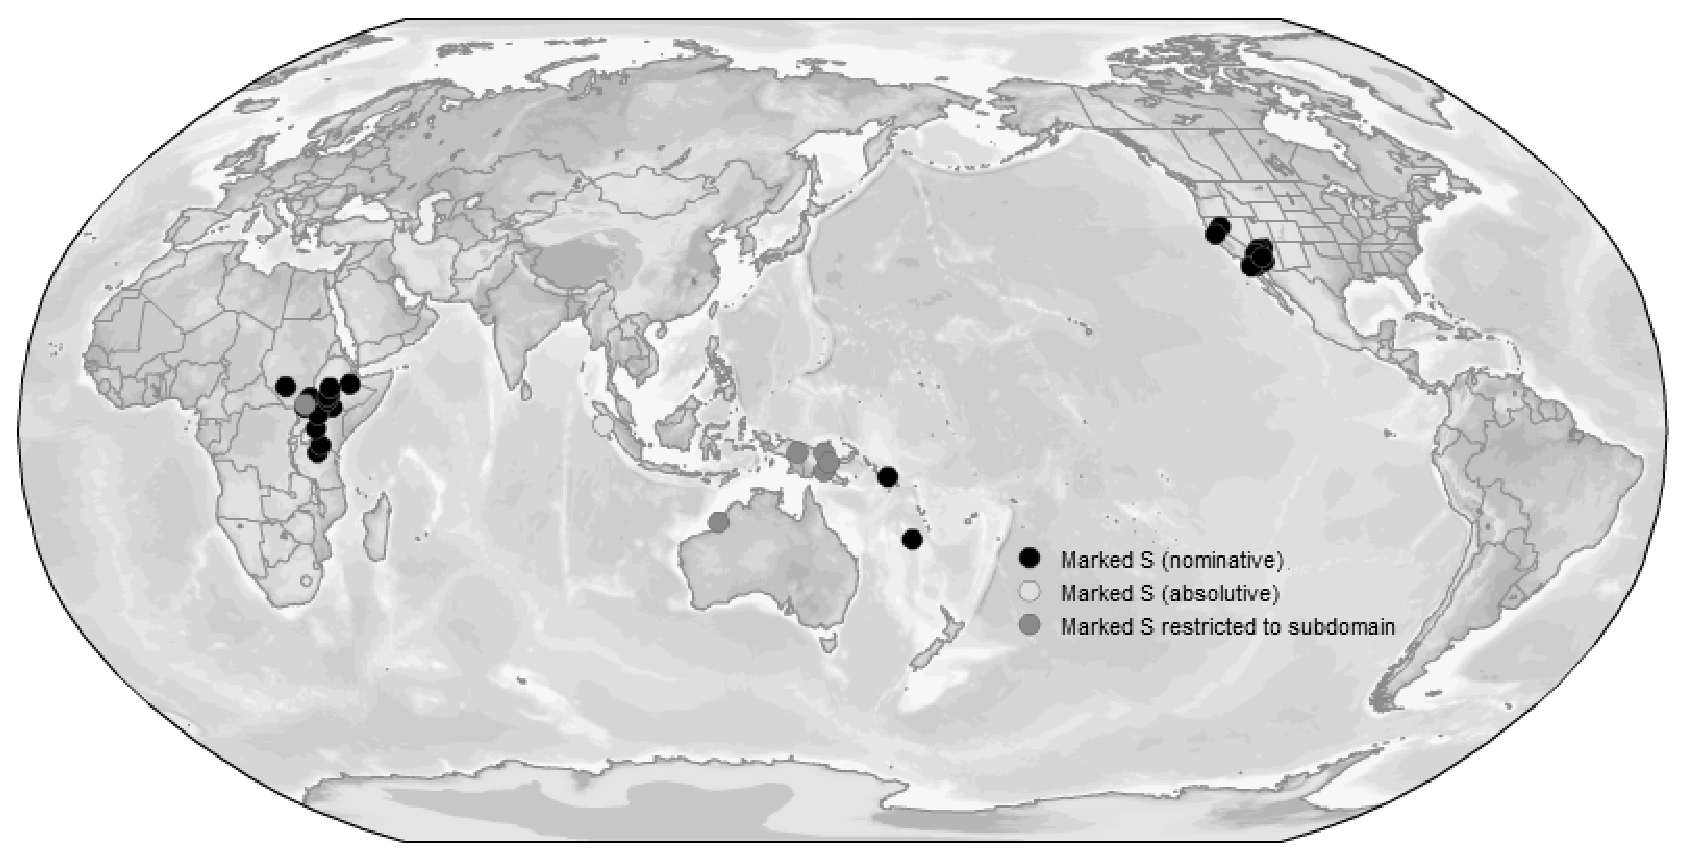
\includegraphics[scale=0.45]{MapFullABW}%
}}%
\caption{Distribution of the languages studied in Chapters 3--7}\label{MapFullBW}
\end{figure}

%An overview table summarizing all roles discussed in this study and all languages is provided at the end of this chapter. 
Figure~\ref{MapFullBW} shows the distribution of all languages that have been discussed at some stage in Chapters~\ref{nompred} to~\ref{extrasyn}.\footnote{The maps shown in this chapter were generated with the interactive tool of the \textit{World Atlas of Language Structures} \citep{WALS}, which was developed by Hans-J\"org Bibiko.} 
Out of these 33 languages, ten languages have data for less than half of the  roles on which data has been collected (the number of roles studied is 17 in total, including the transitive roles of A and P). 
These languages are not included in the following.\footnote{The languages which have been excluded from the analysis in the present chapter are all of the Pacific languages with the marked"=S pattern only for emphatic\is{emphatic subject} subjects discussed in Chapter~\ref{emphaticS}, namely Eipo\il{Eipo}, Kaki Ae\il{Kaki Ae}, Nabak\il{Nabak}, Waskia\il{Waskia} and Yawuru\il{Yawuru}. In addition, the Yuman languages Cocopa\il{Cocopa}, Maricopa\il{Maricopa} and Walapai\il{Walapai} have been excluded due to lack of data, as well as the Nilotic languages P\"ari\il{P\"ari}, which has the marked"=S pattern only in some non-basic clauses, and Dinka\il{Dinka (Agar)}.} 
The remaining 23 languages are visualized on the map in Figure~\ref{MapReduxBW}.

\begin{figure}[htbp] \centering \resizebox{\textwidth}{!}{\fbox{%
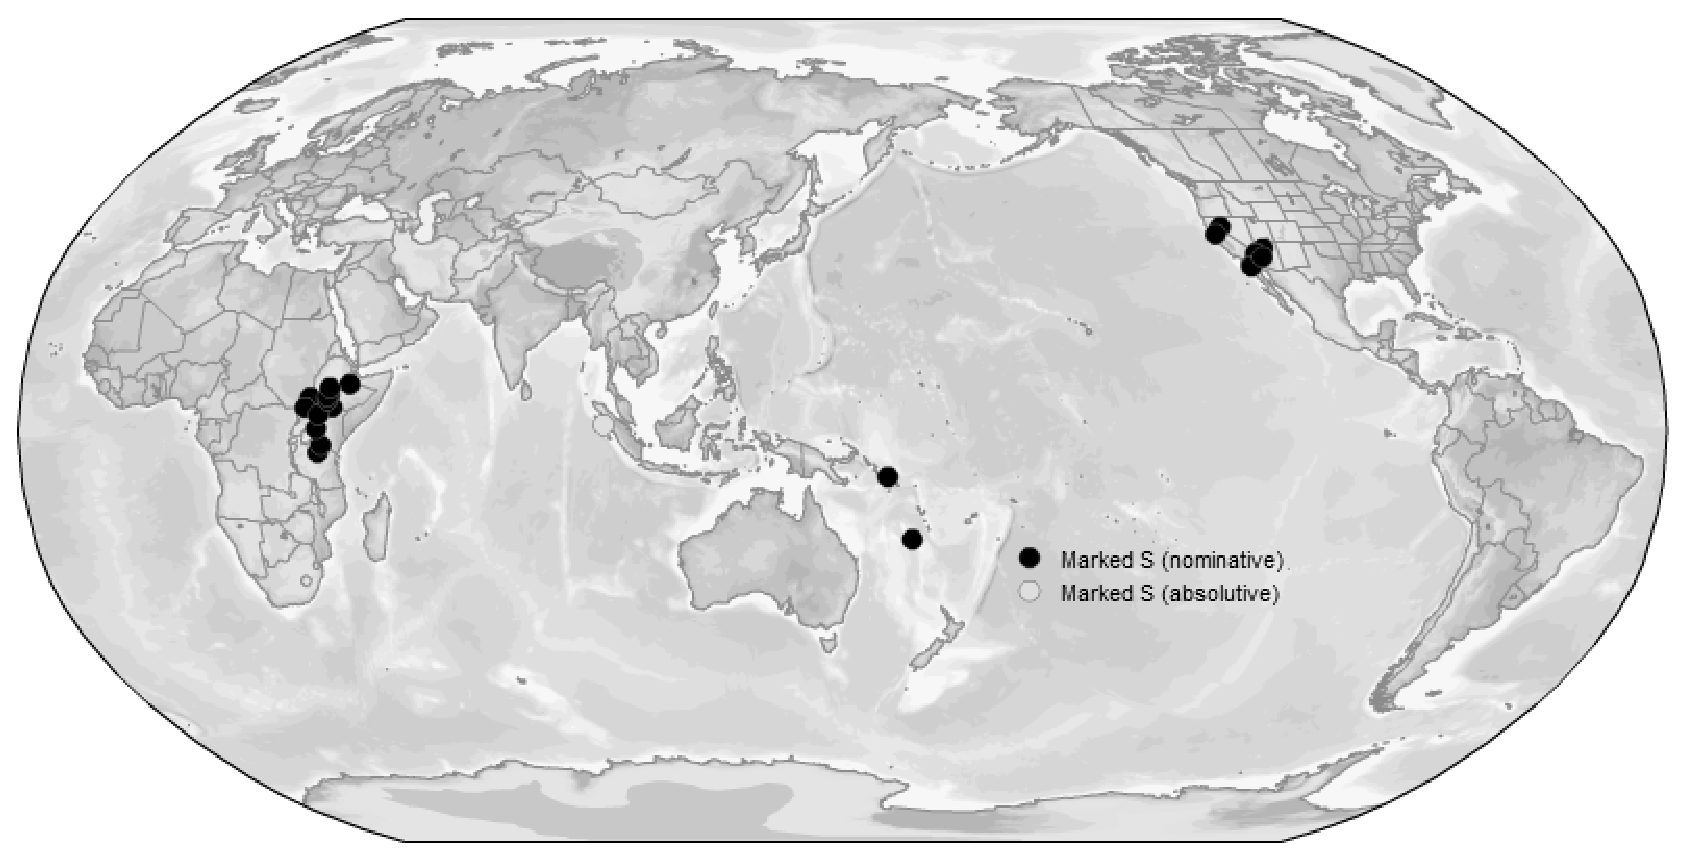
\includegraphics[scale=0.45]{MapReduxBW}}%
}%
\caption{Distribution of the languages used for comparison}\label{MapReduxBW}
\end{figure}


The data collected in this study provides information on the encoding of individual roles in individual languages. 
Both types of entities, i.e. roles and languages, can be used as the means of comparison, and indeed both will be used in the next sections.
In the remainder of this section I will discuss the two means of comparison. 
The language level will be discussed first, followed by the role level. 

When\is{typology!sampling!genealogical grouping|(} making typological generalizations over a number of languages, one runs into a problem when trying to arrive at meaningful results.
Statistical analysis of the data demands independence of the data. 
This criterion is, however, not necessarily met by language data that comes from related languages; and, as \citet{Dryer:1989} remarks, all languages in the world might well be related to one another.
If a sample of languages contains a large number of related languages sharing a linguistic feature (potentially due to their common origin), this feature might wrongly be shown to be a significantly preferred across the world's languages, though in fact this preference only holds for the respective genealogical grouping. 
This and related problems are discussed in \citet{Dryer:1989} and \citet{Bickel.samp}; these two papers also propose solutions on how to avoid misinterpretation of typological preferences.
In short, the suggested solutions propose genealogical (and also areal) control of samples, even though if taken to the extreme, this procedure can lead to very small sample sizes, leading to other statistical difficulties. 

\enlargethispage{\baselineskip}
Two questions arise when attempting to balance data sets according to genealogy (and areal distribution).
First, between which groupings of languages can relative independence of the data be expected, and second, how does one then proceed to balance the data between those groupings in the analysis.
\citet[267]{Dryer:1989} proposes the genus as the level of relatedness above which one can assume relative independence of data points, though he notes that different linguistic features have different levels of stability and therefore some features might be considered independent on a smaller or larger time scale. 
Accordingly, with this the data will be analyzed on the genus level in addition to the analysis based on individual languages.
The genera used in this study are taken from the classification used in \citet{WALS}. 
Different methods are available to balance the data with respect to the groups one has established for the analysis. 
The first possibility is to pick a representative language for each of the defined groups and use the data of this language. 
However, based on the language choice, the data representing a group of languages might not be representative for the group as a whole.
Another possibility is to include more languages for each group in order to take into account in-group variation but to weight the data of the individual groups with respect to each other in the later analysis. This procedure provides `controlled genealogical sampling' \citep{Bickel.samp}. 
I have chosen a similar method for analyzing marked"=S languages on a genealogically controlled level (though the details differ from \citeauthor{Bickel.samp}'s proposal). 
For each role that is investigated, an average figure of the encoding-pattern has been calculated based on the languages of the respective genealogical grouping. 
The same has also been done to determine the coding-pattern of the individual languages in case they allow for alternative constructions to encode a certain role. 
Both types of data, based on individual language data and grouped genealogically, are presented in the following, and the results are compared.\is{typology!sampling!genealogical grouping|)}
 
In addition to the distinction between the level of individual languages and genus, another contrast is made in my analysis of marked"=S languages.
For each dataset, I provide two types of coding. 
In Section~\ref{explain}, I\is{marked-S languages!functional definition!strong versus weak hypothesis|(} have distinguished between the weak and strong version of the functional explanation of marked"=S. 
In general, the functional hypothesis proposed by \citet{Koenig:2006} lessens the impact of the marking of the S, A and P roles. 
It takes other roles into consideration and states that the overall distribution of the less-coded form (the zero-case in my terminology) should have a wider distribution as the form it corresponds to with respect to the S, A and P encoding would have in non-marked"=S languages. 
What exactly is meant by wider distribution is, however, left a bit vague. 
Two possible interpretations are, first, that the zero-case is used in more contexts than the S-case (weak version) or, second, that the zero-case is used in more contexts than all other (overt) case-forms together (strong version). 
In accordance with these two versions of the hypothesis, I have compared two different encodings of the role-encoding data in marked"=S languages. 
In the first variant, I code whether a role is encoded by the same case-form as the prototypical P or A role (dubbed the zero-case in this study), or as the S+A/P role.
In addition, roles that are coded by neither of the two case-forms are listed in a separate column as `other'. 
The second coding used for the data strictly distinguishes whether a role is encoded by zero-coding or by overt material. 
For many roles, the second coding can be derived from the first coding by adding up the S-case and other case columns. 
However, the zero- versus overt-coding data-representation also includes forms of overt coding other than case-marking.
For example, the genitive particles found in the attributive\is{possession!attributive} possessive construction in many languages (cf. Chapter~\ref{extrasyn}) are represented as overt material.\is{marked-S languages!functional definition!strong versus weak hypothesis|)}

\section{Comparison across roles}\label{rolestyp}

The roles studied in the previous chapters show varying tendencies of behavior similar or dissimilar to that of S arguments in terms or their overt coding.
While all of the roles are found to be encoded with the S-case in at least one language of my sample, the proportions of S-like and non-S-like encoding exhibit wide variation between the individual roles. 
While subjects of locational\is{locational predication} clauses are almost always encoded like standard intransitive subjects of a language, the form used in citation\is{citation form} is only encoded in this way as an alternative strategy in one language, namely Nias\il{Nias} (a behavior that most likely is a very recent innovation).  
Further, for the roles investigated, if a case-form other than the S-case is chosen, then the zero-case is the most likely alternative, although this varies between the roles, too. 
For attributive\is{possession!attributive} possessors, the tendency to choose the zero-coded case is equally strong as the tendency to employ a special overtly coded case-form, a genitive. 
These findings apply to the total set of individual languages as well as to a genealogically controlled sample.
In this section I will discuss these results in more detail. 

%language level, roles as coded by case function (S,A,P other)
 
\begin{table}[h,t,b]
\centering
\begin{tabular}{lccccccc}
\hline \hline
\bfseries role &\multicolumn{2}{c}{\bfseries $\emptyset$-case} &\multicolumn{2}{c}{\bfseries S-case} &\multicolumn{2}{c}{\bfseries other}&\bfseries total \\
{}&No.&\%&No.&\%&No.&\%& \bfseries languages\\
\hline
S argument &0  &0\,\% &23  &100\,\%  &0  &0\,\% & 23\\
%\hdashline
Locational S &0.5  &2\,\% &21.5  &98\,\% &0  &0\,\% &22\\
%\hdashline
%%%S VIC&1  &7\,\% &13  &93\,\% &0  &0\,\% &14\\
%%%%% \hdashline
S VDC&3.5  &23\,\%  &11.5  &77\,\% &0  &0\,\% &15\\
%\hdashline
Positive existentials&4.5  &23\,\% &14.5  &73\,\% &1  &5\,\% &20\\
%\hdashline
Adverbial clauses&2  &22\,\% &6.5  &72\,\% &0.5  &6\,\% &9\\
%\hdashline
Nominal predication&7  &33\,\% &14  &67\,\% &0  &0\,\% &21\\
%\hdashline
Negative existentials&4  &40\,\% &6  &60\,\% &0  &0\,\% &10\\
%\hdashline
Relative clauses&6  &35\,\% &10  &59\,\% &1  &6\,\% &17\\
%\hdashline
Emphatic S&7  &41\,\% &8  &47\,\% &2  &12\,\% &17\\
%\hdashline
Complement clause&3  &60\,\% &2  &40\,\% &0  &0\,\% &5\\
%\hdashline
Predicate nominal&17  &77\,\% &4  &18\,\% &1  &5\,\% &22\\
%\hdashline
Term of address&8.5  &65\%  &0.5  &4\% &4  &31\% &13\\
%\hdashline
Attributive possessor&10  &43.5\,\%  &1  &4\,\% &12  &52\,\% &23\\
%\hdashline
Citation form&22.5  &98\,\% &0.5  &2\,\% &0  &0\,\% &23\\
\hline \hline
\end{tabular}
\caption{Overview on percentage of zero-case and S-case-marking for different roles}\label{SumRoleLang}
\end{table}

Table~\ref{SumRoleLang} lists the roles studied. 
For each role, it is indicated which percentage of the languages uses a certain case-form. 
Three different case values are distinguished, namely the zero-case, the S-case and other, if a different case-form altogether is used for the respective role. 
If a language uses more than one strategy for a role, both patterns are included and a mean score from all different constructions is listed for the encoding of the role. 
If, for example, a language has two constructions that encode a context and the relevant role is encoded using the S-case in the first construction and the zero-case in the second construction, this role is represented with the value 0.5 in both columns.  
The roles are listed in decreasing order according to the percentage the S-case is used for encoding.\footnote{The percentages have been rounded to full integers in the following. Therefore, the values in one row of the table add up to 101\,\% instead of 100\,\% for some rows.}

The data in table~\ref{SumRoleLang} show that the role that behaves most like intransitive S arguments in terms of overt coding is the subject of locational\is{locational predication} clauses. 
This role is marked with the S case in 98\,\% of the languages, while it is encoded with the zero case in only 2\,\%. 
On the other end of the scale is the citation form\is{citation form} of a noun. 
Figures for this role are the reverse of those of the locational\is{locational predication} subject, with 2\,\% being encoded with the S-case and 98\,\% with the zero-case. 
In between these two extremes, the other roles line up. 
The non-clause-level roles all have percentages below five for the S-case encoding, but they still differ in their encoding behavior. 
While the citation\is{citation form} form, as mentioned above, almost exclusively makes use of the zero-case, half of the attributive\is{possession!attributive} possessors are encoded by a different case-form altogether, and roughly the other half is encoded by the zero-case. 
Terms of address\is{terms of address} are located in between these to patterns with roughly a third of the languages using a different case-form altogether, and about two thirds using the zero-case. 
 
There are a number of roles that behave more like intransitive S arguments in terms of their encoding.
In addition to subjects of locational\is{locational predication} clauses, most roles that will be subsumed under the subject category in most grammars are encoded like intransitive S arguments quite regularly. Subjects of %valency-increasing (93\,\%) and 
valency-decreasing\is{valency-decreasing construction} constructions (77\,\%), positive existential\is{existential predication} constructions (73\,\%), adverbial clauses (72\,\%) and nominal predications\is{nominal predication!subject of} (67\,\%) are regularly marked with the same case as prototypical S arguments in two thirds of the languages in the sample or more. 
Negative existential constructions\is{existential predication} (60\,\%) and relative clauses (59\,\%) still use the S-case in more than half of the cases. 
Emphatic\is{emphatic subject} subjects (47\,\%) and complement clauses (40\,\%) are encoded like typical S arguments in just below fifty percent of the languages.
Finally, predicate nominals\is{nominal predication!predicate nominal} (18\,\%) are seldom encoded in the S-case in marked"=S languages. 
This role is similar to the non-clause-level roles since it does not represent a type of subject.

%language level, roles compared by coding (overt/ zero)

\begin{table}[h,t,b]
\centering
\begin{tabular}{lccccc}
\hline \hline
\bfseries role &\multicolumn{2}{c}{\bfseries zero-coding} &\multicolumn{2}{c}{\bfseries overt coding} &\bfseries total \\
{}& No.&\%&No.&\%& \bfseries languages\\
\hline
S argument &0  &0\,\% &23  &100\,\%  & 23\\
%\hdashline
Locational S &0.5  &2\,\% &21.5  &98\,\% &22\\
%\hdashline
%%%%%%S VIC&1  &7\,\% &13  &93\,\% &14\\
%%%%%%% \hdashline
S VDC&2.5  &17\,\%  &12.5  &83\,\% &15\\
%\hdashline
Adverbial clauses&2  &2\,\% &7  &78\,\% &9\\
%\hdashline
Positive existentials&4.5  &23\,\% &15.5  &78\,\% &20\\
%\hdashline
Emphatic S&5  &29\,\% &12  &71\,\% &17\\
%\hdashline
Nominal predication&7  &33\,\% &14  &67\,\% &21\\
%\hdashline
Relative clauses&6  &35\,\% &11  &65\,\% &17\\
%\hdashline
Negative existentials&4  &40\,\% &6  &60\,\% &10\\
%\hdashline
Attributive possessor&10  &43\,\%  &13  &57\,\% &23\\
%\hdashline
Complement clause&3  &60\,\% &2  &40\,\% &5\\
%\hdashline
Term of address&8.5  &65\,\%  &4.5  &35\,\% &13\\
%\hdashline
Predicate nominal&17  &77\,\% &5  &23\,\% &22\\
%\hdashline
Citation form&22.5  &98\,\% &0.5  &2\,\% &23\\
\hline \hline
\end{tabular}
\caption{Overview on percentage of zero versus overt coding for different roles}\label{SumRoleLangZero}
\end{table}

Table~\ref{SumRoleLangZero} distinguishes whether a role is coded through overt marking or without any overt material. 
As noted above (Section~\ref{general}), other overt material such as particles has been included here, so that the figures for the zero-case in Table~\ref{SumRoleLang} and the zero-coded in this table do not always coincide. 
The two extremes are the same as in the previous table, with subjects of locational\is{locational predication} clauses being overtly coded in 98\,\% of the cases and the citation form\is{citation form} being overtly coded in only 2\,\%. 
The roles that make frequent use of case-forms other than the S-case or zero-case end up in different positions than in the previous table. 
Attributive\is{possession!attributive} possessors (57\,\% of overt coding versus 4\,\% of S-case-marking) and terms of address\is{terms of address} (35\,\% vs. 4\,\%) are found in a higher position of the table accordingly. 
Also, roles that are encoded via constructions that include additional overt (but non-case) morphology on the respective roles have been affected. 
Again, the attributive\is{possession!attributive} possessor is subject to this (due to encoding with genitive particles) and also the emphatic\is{emphatic subject} S role, which has a figure of 71\,\% overt coding as compared to 47\,\% of S-case-marking. 
In some other cases, the addition of the roles marked by other cases have led to minor changes in positioning since Table~\ref{SumRoleLang} is ordered according to the percentage of S-case-marking.
Apart from these deviations, the ranking of roles remains stable between the two tables. 
This indicates that there is only a slight difference in the results, depending on whether one tests the weak of strong version\is{marked-S languages!functional definition!strong versus weak hypothesis} of the functional marked"=S hypothesis. 
Moreover, the results differ only for a subset of roles.

In the two following tables, the same data is presented, but now the level of comparison is not the number of languages that encode a particular role in a given way, but the genus level. 
The languages of my sample belong to 10 different genera. 
The data represents the Nilotic and Surmic languages (both of the Nilo-Saharan family), Eastern Cushitic and Omotic (both Afro-Asiatic) and the Yuman languages. 
Furthermore, there are five languages that do not have any closely-related languages within the sample and thus are the only representatives of their family. 
These languages are Nias\il{Nias} (Sundic), Aji\"e\il{Aji\"e} (Oceanic), both of the Austronesian family, Savosavo\il{Savosavo} (Solomons East Papuan), Maidu\il{Maidu} (Maidu\il{Maidu}an) and Wappo\il{Wappo} (Wappo\il{Wappo}). 
For the languages that are the single representative of their genus, their data has been used to represent the respective genus. 
For genera with more than one representative, an average figure has been calculated for each role.  

% genus level comparison by case function (SAP other)
\begin{table}[t,b,h]
\centering
\begin{tabular}{lccccccc}
\hline \hline
\bfseries role &\multicolumn{2}{c}{\bfseries $\emptyset$-case} &\multicolumn{2}{c}{\bfseries S-case} &\multicolumn{2}{c}{\bfseries other}&\bfseries total \\
{}&No.&\%&No.&\%&No.&\%& \bfseries genera\\
\hline
S argument &0  &0\,\% &10  &100\,\%  &0  &0\,\% & 10\\
%\hdashline
Locational S &0.5  &5\,\% &9.5  &95\,\% &0  &0\,\% &10\\
%\hdashline
%%%%%%S VIC&0.5  &6\,\% &8.5  &94\,\% &0  &0\,\% &9\\
%%%%%% \hdashline
Positive existentials&1.9  &19\,\% &7.8  &78\,\% &0.3  &3\,\% &10\\
%\hdashline
S VDC&1.8  &23\,\% &6.2  &77\,\% &0  &0\,\% &8\\
%\hdashline
Adverbial clauses&1  &20\,\% &3.5  &70\,\% &0.5  &10\,\% &5\\
%\hdashline
Nominal predication&3  &33\,\% &6  &66\,\% &0  &0\,\% &9\\
%\hdashline
Negative existentials&3.3  &42\% &4.7  &58\% &0  &0\% &8\\
%\hdashline
Relative clauses&3  &38\,\% &4  &50\,\% &1  &13\,\% &8\\
%\hdashline
Emphatic S&4.6  &46\,\% &4.9  &49\,\% &0.5  &5\,\% &10\\
%\hdashline
Complement clause&3  &60\,\% &2  &40\,\% &0  &0\,\% &5\\
%\hdashline
Predicate nominal&8  &80\,\% &1.8  &18\,\% &0.3  &3\,\% &10\\
%\hdashline
Attributive possessor&3  &30\,\% &1  &10\,\% &6  &60\,\% &10\\
%\hdashline
Term of address&6  &67\,\% &0.5  &6\,\% &2.5  &28\,\% &9\\
%\hdashline
Citation form&9.5  &95\,\% &0.5  &5\,\% &0  &0\,\% &10\\
\hline \hline
\end{tabular}
\caption{Overview on percentage of zero-case and S-case-marking for different roles by genus}\label{SumRoleGen}
\end{table}

The data in Table~\ref{SumRoleGen} is divided into zero-case, S-case and other case. 
It basically shows the same picture as Table~\ref{SumRoleLang}. 
There are only two instances in which the two tables deviate from each other in the absolute rankings of the roles. 
Both attributive\is{possession!attributive} possessors and terms of address\is{terms of address}, as well as subjects of valency-decreasing\is{valency-decreasing construction} constructions and positive existential\is{existential predication} predication have switched positions.
Otherwise, the rankings are identical.
Apart from these minor variations in ordering, there are some differences between the language and genus level in terms of the individual percentages. 
This is due to the fact that the total number of genera is only 10, which increases the overall percentage of rarely attested patterns that are found in genera with only a few or a single member within the sample. 
These data have been organized into zero and overt coding in Table~\ref{SumRoleGenOvert}.

%family level comparison by coding relation (overt vs. zero)
\begin{table}[t,b,h]
\centering
{
\begin{tabular}{lccccc}
\hline \hline
\bfseries role &\multicolumn{2}{c}{\bfseries zero-coding} &\multicolumn{2}{c}{\bfseries overt coding} &\bfseries total \\
{}& No.& \% &No. & \% & \bfseries genera \\
\hline
S argument &0  &0\,\% &10  &100\,\%  & 10\\
%\hdashline
Locational S &0.5  &5\,\% &9.5  &95\,\% &10\\
%\hdashline
%%%%%%S VIC&0.5  &6\,\% &8.5  &94\,\% &9\\
%%%%%%\hdashline
S VDC&1.5  &19\,\% &6.5  &81\,\% &8\\
%\hdashline
Positive existentials&1.9  &19\% &8.1  &81\% &10\\
%\hdashline
Adverbial clauses&1.25  &25\,\% &3.75  &75\,\% &5\\
%\hdashline
Attributive possessor&3  &30\,\% &7  &70\,\% &10\\
%\hdashline
Nominal predication&3  &33\,\% &6  &67\,\% &9\\
%\hdashline
Emphatic S&3.3  &33\,\% &6.7  &67\,\% &10\\
%\hdashline
Relative clauses&3  &38\,\% &5  &63\,\% &8\\
%\hdashline
Negative existentials&3.3  &42\,\% &4.7  &58\,\% &8\\
%\hdashline
Complement clause&3  &60\,\% &2  &40\,\% &5\\
%\hdashline
Term of address&6  &67\,\% &3  &33\,\% &9\\
%\hdashline
Predicate nominal&8  &80\,\% &2  &20\,\% &10\\
%\hdashline
Citation form&9.5  &95\,\% &0.5  &5\,\% &10\\
\hline \hline
\end{tabular}
}
\caption{Overview on percentage of zero versus overt coding for different roles by genus}\label{SumRoleGenOvert}
\end{table}

The relation between Table~\ref{SumRoleGenOvert} and Table~\ref{SumRoleLangZero} is not as straightforward as between the two tables that have just been compared. 
The majority of roles have kept an identical or almost identical position between the two tables. 
However, there is one notable difference. 
The attributive\is{possession!attributive} possessor scores four positions higher on the genus level than on the language level. 
This indicates that languages that use the zero-case for this role are somewhat overrepresented in the sample. 
All other roles have the same rank between the two levels of comparison or deviate only by one position. 
Roles that show this minimal variation between the two tables are adverbial clauses and positive existential\is{existential predication} predications as well as subjects of nominal predications\is{nominal predication!subject of} and emphatic\is{emphatic subject} subjects; both pairs have switched positions between the two tables. 
As in the previous table, though, the ranking is rather stable for the language and genus level as with respect to overt versus zero-coding, the individual percentages differ occasionally.

Finally, comparing the data on genus level for the encoding as zero-case, S-case and other with the encoding as overt versus zero-coding a number of deviations between the rankings can be found. 
The attributive\is{possession!attributive} possessor is six positions lower in Table~\ref{SumRoleGen} than in Table~\ref{SumRoleGenOvert}. 
This has also been the biggest difference on language level between the two encodings. 
Subjects of negative existentials\is{existential predication}, meanwhile, score two positions higher in the first table if one takes into account the intervening attributive\is{possession!attributive} possessor (otherwise the difference is three positions). 
Again, taking into account, the already mentioned differences, three more minor deviations in terms of pairwise switching of positions exist between the two tables. 
These pairs of roles are: subjects of valency-decreasing\is{valency-decreasing construction} constructions and positive existential\is{existential predication} predications; emphatic\is{emphatic subject} subjects and subjects of relative clauses; as well as terms of address\is{terms of address} and predicate\is{nominal predication!predicate nominal} nominals. 

\section{Comparison across languages}\label{languagestyp}

While the previous section analyzed the data from the perspective of the different roles investigated in this study, this section takes a closer look at the different marked"=S languages. 
More precisely, the similarities and differences in encoding of the respective roles are investigated. 
Again, both types of encoding have been taken into account. 
The first type distinguishes between coding in terms of zero-case (i.e. P/A coding) versus S(+A/P)-case versus other case-form. 
The second type strictly differentiates between overt and zero-coding.
Even though in the last section the data on individual versus genus level has proved to be almost identical, this section analyzes the data from both the language and the genus level. In addition, for each language its genus is listed in the language level tables and the overall similarity within the individual genera is discussed.

\begin{table}[t,b,h]
\resizebox{\textwidth}{!}{
\begin{tabular}{lccccccc}
\hline \hline
\bfseries language &\multicolumn{2}{c}{\bfseries $\emptyset$-case} &\multicolumn{2}{c}{\bfseries S-case} &\multicolumn{2}{c}{\bfseries other}&\bfseries total\\
{} &  No. & \% & No. &\% & No.&\% & \bfseries roles\\
\hline
Diegue\~no\il{Diegue\~no (Mesa Grande)} (Mesa Grande), Yuman &8  &67\,\%  &4  &33\,\%  &0  &0\,\% & 12\\
%\hdashline
Aji\"e\il{Aji\"e}, Oceanic&7  &58\,\% &4.5  &38\,\% &0.5  &4\,\% &12\\
%\hdashline
Datooga, Nilotic&7  &58\,\% &5  &42\,\% &0  &0\,\% &12\\
%\hdashline
Maa\il{Maa}, Nilotic& 6  &50\,\% & 6  &50\,\% &0  &0\,\% & 12\\
%\hdashline
Jamul\il{Jamul Tiipay} Tiipay, Yuman&7.5  &58\,\% &5.5  &42\,\% &0  &0\,\% &13\\
%\hdashline
Wappo\il{Wappo}, Wappo\il{Wappo}&8  &50\,\% &7  &44\,\% &1  &6\,\% &16\\
%\hdashline
Nias\il{Nias}, Sundic&7.5  &54\,\% &6.5  &46\,\% &0  &0\,\% &14\\
%\hdashline
Oromo (Boraana\il{Oromo (Boraana)}), Eastern Cushitic&5  &45\,\% &5  &45\,\% &1  &9\,\% &11\\
%\hdashline
Mojave\il{Mojave}, Yuman&7  &44\,\% &9  &56\,\% &0  &0\,\% &16\\
%\hdashline
Havasupai\il{Havasupai}, Yuman&4.5  &45\,\% &5.5  &55\,\% &0  &0\,\% &10\\
%\hdashline
Savosavo\il{Savosavo}, Solomons East Papuan&6.5  &43\,\% &6  &40\,\% &2.5  &17\,\% &15\\
%\hdashline
Tennet, Surmic&5.5  &42\,\% &6.5  &50\,\% &1  &8\,\% &13\\
%\hdashline
Turkana\il{Turkana}, Nilotic&6  &40\,\% &7  &47\,\% &2  &13\,\% &15\\
%\hdashline
Yavapai\il{Yavapai}, Yuman&5  &39\,\% &8  &62\,\% &0  &0\,\% &13\\
%\hdashline
Nandi\il{Nandi}, Nilotic&4.5  &38\,\% &7.5  &63\,\% &0  &0\,\% &12\\
%\hdashline
Zayse\il{Zayse}, Omotic&3  &33\,\% &5  &56\,\% &1  &11\,\% &9\\
%\hdashline
Murle\il{Murle}, Surmic&4  &33\,\% &7  &58\,\% &1  &8\,\% &12\\
%\hdashline
Arbore\il{Arbore}, Eastern Cushitic&3 &30\,\% &5  &50\,\% &2  &20\,\% &10\\
%\hdashline
Wolaytta\il{Wolaytta}, Omotic&2.5  &28\,\% &4.5  &50\,\% &2  &22\,\% &9\\
%\hdashline
Oromo  (Harar\il{Oromo (Harar)}), Eastern Cushitic&3  &23\,\% &7  &54\,\% &3  &23\,\% &13\\
%\hdashline
Gamo\il{Gamo}, Omotic&3  &23\,\% &8  &62\,\% &2  &15\,\% &13\\
%\hdashline
K'abeena\il{K'abeena}, Eastern Cushitic&3.5  &23\,\% &10  &67\,\% &1.5  &10\,\% &15\\
%\hdashline
Maidu\il{Maidu}, Maidu\il{Maidu}an&2.5  &23\,\% &7.5  &68\,\% &1  &9\,\% &11\\
\hline \hline
\end{tabular}}
\caption{Overview on percentage of zero-case and S-case-marking for different languages}\label{SumLang}
\end{table}


% Notes on language comparison: 
I have ranked the languages in Table~\vref{SumLang} with respect to the percentage of roles covered by the zero-case from high to low.
The scores range from 67\,\% of roles being coverd by the zero-case to a 23\,\% coverage. 
These data show that languages of the marked"=S type do not behave in a uniform way. 
Furthermore, while some languages indeed have a wide range of contexts in which the zero-case is used, some marked"=S languages do so only rarely.
The languages which make use of the zero-case to a lesser degree, however, often employ other overtly coded case-forms than the S-case for the roles studied here.  
Remember that in some of the languages both case-forms, the zero-case and the S-case, are overtly coded. 
The `unmarked' status of the zero-case is justified by its use in extra-syntactic contexts in these languages. 
The Omotic languages are of this type of marked"=S language. 
Interestingly, these languages appear to make little use of the zero-case in comparison with other marked"=S languages and thus are found near the bottom end of Table~\ref{SumLang}. This is especially obvious for Gamo\il{Gamo}, which is the Omotic language with the best data coverage in the sample. 
Since the total number of contexts that employ the zero-case in the related languages is equally low, the higher percentage of use of the zero-case given for Zayse\il{Zayse} and Wolaytta\il{Wolaytta} are probably a result of their small number of contexts attested.  
Most languages of a genus tend to be scattered over roughly the same region of the table. 
While the Omotic languages are found in the lower half of the table, the Yuman languages are located in the upper half. 
The Eastern Cushitic languages, except for Boraana\il{Oromo (Boraana)} Oromo, are found in the lower ranks as well. 
The Surmic languages (Tennet and Murle\il{Murle}) score in the lower mid region of the table. 
Only the Nilotic languages are mixed with two languages (Datooga and Maa\il{Maa}) located close to the top of the table and two other languages (Turkana\il{Turkana} and Nandi\il{Nandi}) in the lower middle of the ranking. 
Notably, these groupings do not reflect the genealogical grouping within the Nilotic languages but rather appear to be a reflex of the languages' geographical location.\footnote{Genealogically, Maa\il{Maa} and Turkana\il{Turkana} group together as East Nilotic and Datooga and Nandi\il{Nandi} as South Nilotic. The geographical distribution of the languages will be discussed later in Section~\ref{area}. The curious reader may skip ahead to Figure~\ref{MapAfrica} for a map of the East African marked"=S languages.}  
Of the languages in the sample that are the single representative of their genus, the two Austronesian languages Nias\il{Nias} (Sundic) and Aji\"e\il{Aji\"e} (Oceanic) are among the highest ranked, together with North-American Wappo\il{Wappo}; all these languages use the zero-case for half of the roles studied or more. 
Non-Austronesian Savosavo\il{Savosavo} scores just above the middle of the ranking. 
Finally, Maidu\il{Maidu} is located near the bottom end among the Omotic and Eastern Cushitic languages of the Afro-Asiatic family.

%by genus

\begin{table}[t,b,h]
\centering
\begin{tabular}{lccccccc}
\hline \hline
\bfseries genus &\multicolumn{2}{c}{\bfseries $\emptyset$-case} &\multicolumn{2}{c}{\bfseries S-case} &\multicolumn{2}{c}{\bfseries other}&\bfseries total\\
{} &No.&\% &No. &\% &No. &\% &\bfseries roles\\
\hline
Oceanic&7  &58\,\% &4.5  &38\,\% &0.5  &4\,\% &12\\
%\hdashline
Sundic&7.5  &54\,\% &6.5  &46\,\% &0  &0\,\% &14\\
%\hdashline
Wappo\il{Wappo}&8  &50\,\% &7  &44\,\% &1  &6\,\% &16\\
%\hdashline
Nilotic&7.2  &48\,\% &7  &47\,\% &0.8  &5\,\% &15\\
%\hdashline
Yuman&7  &44\,\% &9 &56\,\% &0  &0\,\% &16\\
%\hdashline
Solomons East Papuan&6.5  &43\,\% &6  &40\,\% &2.5  &17\,\% &15\\
%\hdashline
Surmic&6  &43\,\% &7  &50\,\% &1  &7\,\% &14\\
%\hdashline
Eastern Cushitic&4.1  &27\,\% &8.6  &57\,\% &2.3  &16\,\% &15\\
%\hdashline
Maidu\il{Maidu}an&2.5  &23\,\% &7.5  &68\,\% &1  &9\,\% &11\\
%\hdashline
Omotic&2.8  &20\,\% &9.2  &66\,\% &2  &14\,\% &14\\
\hline \hline
\end{tabular}
\caption{Overview on percentage of zero-case and S-case-marking for different genera}\label{SumFam}
\end{table}

Table~\ref{SumFam} summarizes the data organized by genus. For genera that are represented by more than one language the data of the individual languages from the genus has been averaged like in the previous section.
Again the ordering is according to the percentage of roles covered by the zero-case beginning with the highest percentage.
This table repeats the general picture lined out in the previous discussion of the languages.
Oceanic, Sundic and Wappo\il{Wappo}, which are all represented through a single language in the sample, mark the top of the ranking by genus. 
Afterwards, Nilotic, Yuman, Solomons East Papuan, and Surmic follow in the mid-field. And as was to be expected from the data of the individual languages, the ranking is concluded by Eastern Cushitic, Maidu\il{Maidu}an, and Omotic. 
The relatively low ranking of Yuman might be surprising at first glance, since the last table has been topped by a language of this genus. 
However, since the overall number of Yuman languages is the sample is the largest of all genera, its overall impact on the ranking of the whole genus has not been large in the end.
 
%comparison by coding relation (overt vs. zero)

\begin{table}[t,b,h,p]
\centering
\begin{tabular}{lcccccc}
\hline \hline
\bfseries language, genus &\multicolumn{2}{c}{\bfseries zero-coding}  & \multicolumn{2}{c}{\bfseries overt coding} &\bfseries total\\
{} & No. & \%  & No. & \% & {\bfseries roles}\\
\hline
Diegue\~no\il{Diegue\~no (Mesa Grande)}  Mesa Grande, Yuman &8 &67\,\% &4 & 33\,\%& 12\\
%\hdashline
Aji\"e\il{Aji\"e}, Oceanic&7 &58\,\%&5 &42\,\%&12\\
%\hdashline
Datooga, Nilotic&7 &58\,\%&5 &42\,\%&12\\
%\hdashline
Jamul\il{Jamul Tiipay} Tiipay, Yuman&7.5 & 58\,\% &5.5 & 42\,\% &13\\
%\hdashline
Nias\il{Nias}, Sundic&7.5 &  54\,\% &6.5 & 46\,\% &14\\
%\hdashline
Maa\il{Maa}, Nilotic& 6 & 50\,\% & 6 & 50\,\% & 12\\
%\hdashline
Wappo\il{Wappo}, Wappo\il{Wappo}&8 &  50\,\% &8 &  50\,\% &16\\
%\hdashline
Havasupai\il{Havasupai}, Yuman&4.5 &  45\,\% &5.5 & 55\,\% &10\\
%\hdashline
Mojave\il{Mojave}, Yuman&7 & 44\,\% &9 & 56\,\% &16\\
%\hdashline
Tennet, Surmic &5.5 & 42\,\% &7.5 & 58\,\% &13\\
%\hdashline
Turkana\il{Turkana}, Nilotic&6 &  40\,\% & 9 &  60\,\% &15\\
%\hdashline
Yavapai\il{Yavapai}, Yuman&5 &  38\,\% &8 &  62\,\% &13\\
%\hdashline
Nandi\il{Nandi}, Nilotic&4.5 & 38\,\% &7.5 & 63\,\% &12\\
%\hdashline
Savosavo\il{Savosavo}, Solomons East Papuan&5.5 & 37\,\% &9.5 & 63\,\% &15\\
%\hdashline
Zayse\il{Zayse}, Omotic&3 & 33\,\% &6 & 67\,\% &9\\
%\hdashline
Murle\il{Murle}, Surmic&4 &33\,\%&8 &67\,\%&12\\
%\hdashline
Arbore\il{Arbore}, Eastern Cushitic&3 &30\,\%&7 &70\,\%&10\\
%\hdashline
Wolaytta\il{Wolaytta}, Omotic&2.5 &28\,\%&6.5 &72\,\%&9\\
%\hdashline
Oromo (Boraana\il{Oromo (Boraana)}), Eastern Cushitic&3 & 27\,\%&8 &73\,\%&11\\
%\hdashline
K'abeena\il{K'abeena}, Eastern Cushitic&3.5 & 23\,\%&11.5 & 77\,\%&15\\
%\hdashline
Oromo (Harar\il{Oromo (Harar)}), Eastern Cushitic&3 & 23\,\%&10 & 77\,\%&13\\
%\hdashline
Gamo\il{Gamo}, Omotic&3 &23\,\%&10 &77\,\%&13\\
%\hdashline
Maidu\il{Maidu}, Maidu\il{Maidu}an&2.5 &23\,\%&8.5 &77\,\%&11\\
\hline \hline
\end{tabular}
\caption{Overview on percentage of zero-case and overt coding for different languages}\label{SumLangSZ}
\end{table}

The languages are also ranked for the data organized by zero-coding versus overt coding, like has been done with the roles.
The picture for the individual languages, as represented in Table~\ref{SumLangSZ} has not changed in most cases.
The most remarkable difference is the ranking of Boraana\il{Oromo (Boraana)} Oromo, which has fallen 11 positions from rank 8 to 19.  
This is the one language in which the re-coding to overt versus zero-coding has the strongest effect, since Boraana\il{Oromo (Boraana)} Oromo uses overt non-case morphology combined with the zero-case-form for a number of roles.
A smaller re-ranking can be found with Savosavo\il{Savosavo} which falls 4 positions as compared to the previous table.
Like Boraana\il{Oromo (Boraana)} Oromo, Savosavo\il{Savosavo} encodes some roles with overt non-case morphology. 
The other languages occupy identical positions in the two rankings.

%By family

\begin{table}[t,b,h,p]
\centering
\begin{tabular}{lccccc}
\hline \hline
\bfseries language family &\multicolumn{2}{c}{\bfseries $\emptyset$-coding}   & \multicolumn{2}{c}{\bfseries overt coding}  &\bfseries total\\
{}&No.&\%&No.&\%&{\bfseries roles}\\
\hline
Oceanic&7  &58\,\% &5  &42\,\% &12\\
%\hdashline
Sundic&7.5  &54\,\% &6.5  &46\,\% &14\\
%\hdashline
Wappo\il{Wappo}&8  &50\,\% &8  &50\,\% &16\\
%\hdashline
Nilotic&7.2  &48\,\% &7.8  &52\,\% &15\\
%\hdashline
Yuman&7.2  &45\,\% &8.8  &55\,\% &16\\
%\hdashline
Surmic&6  &43\,\% &8  &57\,\% &14\\
%\hdashline
Solomons East Papuan&5.5  &37\,\% &9.5  &63\,\% &15\\
%\hdashline
Eastern Cushitic&3.5  &23\,\% &11.5  &77\,\% &15\\
%\hdashline
Maidu\il{Maidu}an&2.5  &23\,\% &8.5  &77\,\% &11\\
%\hdashline
Omotic&2.8  &20\,\% &11.2  &80\,\% &14\\
\hline \hline
\end{tabular}
\caption{Overview on percentage of zero-coding and overt coding for different genera}\label{SumFamZeroS}
\end{table}

Despite the major difference in ranking seen for Boraana\il{Oromo (Boraana)} Oromo on the language level, on genus level no large rearrangements happen.
Table~\ref{SumFamZeroS} presents the ranking of genera in the zero- versus overt-encoding.
Compared with the ranking of genera based on S-case, zero-case or other case-form represented in Table~\ref{SumFam} above, there are almost no changes.
Only Surmic and Solomons East Papuan have switched positions between the two tables. 
This corresponds to the drop in position by Savosavo\il{Savosavo}, which is the only language of this family in the sample, on the language level. 
The rankings of the other genera remain stable between the two genus level tables.
  
\section{Similarity networks}\label{networkstyp}\is{phylogenetic networks|(}

The two previous sections have compared the micro-alignment data from languages of the marked"=S type as defined in Chapter~\ref{method}.
Two different perspectives have been chosen, the similarity/difference between the pre-defined contexts and between the individual languages. 
For each of the scenarios, I have established a ranking from the most S-like context to the least S-like contexts or the language which makes the widest/narrowest use of the zero-case-form respectively.
These ranking are very easy to interpret, but they reduce a complex and potentially multi-dimensional data set to a linear order.
A more sophisticated and mathematically more complex way to analyze the data are (phylogenetic) networks.
The algorithms used to calculate these networks were originally developed to analyze and compare gene sequences of biological species, however, the basic mechanisms can also be used for comparison of linguistic data. 
Phylogenetic networks are generalized versions of tree-structures that allow the inclusion of conflicting information into tree-structures.
In comparison with the linear ordering of the tables presented in the previous sections, these tree-like manifestations allow the addition of another dimension to the data analysis.
If, for instance, half of the languages of the sample use the zero-case for role A and the other half of the sample uses the zero-case for role B, a linear ranking based on percentages would show these contexts next to each other in the ranking. 
This might be interpreted as a relation between roles A in B given only the linear ranking. 
However, in the scenario described above, there is no similarity between the two roles.\footnote{In this made up example, there is in fact a negative correlation between the two roles. However, as the statistically inclined reader will be well aware of, correlations, be they positive or negative, do not imply causation. 
Also, such clear-cut distributions as described in the scenario above, are unlikely to occur in naturalistic data.} 
A similarity network can visualize this difference between the two roles that would appear to behave identical in a table ranked by percentages.
In the following, I will give a brief introduction to interpreting similarity networks. 
However, it should be kept in mind that although they can be a visual aid to discover interesting relationships within data sets, a lot of complexity has to be reduced for the visual representation and thus they are not devoid of artifacts.  
Afterwards, I will present and discuss the networks generated from the data on marked"=S languages. 
It has been demonstrated in the two proceeding sections that there is no big difference in the
results between the encoding of the roles as either zero-case, S-case and other case-form, or zero
versus overt encoding.
%\enlargethispage{2\baselineskip}
In this section, I have therefore chosen to only analyze one kind of data encoding. 
The data sets which have been chosen are the ones that distinguish between zero-case, S-case and other case-forms. 
This data represents the weak form of the functional marked"=S hypothesis (marked"=S languages should encode more roles with the zero-case than with the S-case-form). 
If the weak hypothesis does not arrive at any meaningful results, the stronger version will likely fail to do so as well. 

The\is{NeighborNet|(} graphs in this section have been produced by NeighborNet, a neighbor joining algorithm that produces phylogenetic networks.\footnote{I am very grateful to Michael Cysouw, who helped me with producing the NeighborNet networks.} 
The algorithm is described in \citet{NeighborNet}; a more detailed discussion on the analysis of genealogical data through split networks is given in \citet{NeighborNetApplication}.  
The traditional method of representing phylogenetic relationships, be they for species or human languages, is the (phylogenetic) tree.
However, due to vertical transfer, missing data, and other factors, it is not always possible to construct a perfect treelike structure from data sets.
Network structures can include conflicting data and thus are a good choice to represent linguistic data.
For this study, the reconstruction of prehistory is not much of an issue.
The mechanisms used for constructing genealogical trees can, however, equally well be used to analyze data sets with respect to how similar/diverse the individual taxa are.  
Traditional tree-building methods join two neighboring nodes and amalgamate them to a single node.
Instead, NeighborNet joins three neighboring nodes and combines them to form two superior nodes.
While points of divergence between the taxa are represented through the bifurcations at the respective mother node in a tree, in the network a split is represented through a set of parallel edges. 
In general it can be said that the more treelike a part of the network looks, i.e. by clearly branching of from the rest of the network, the clearer the split is.\is{NeighborNet|)}  

%\begin{figure}[ht] \centering \fbox{
%\includegraphics[scale=0.8]{rolesgenuszeros2}
%}
%\caption{Network of zero-case and S-case-marking for different roles by genus}\label{NetRoleGenZero}
%\end{figure}

\begin{figure}[h,t,b,p] \centering \resizebox{\textwidth}{!}{\fbox{%
\includegraphics%[scale=0.7]
{categoriesSansVIC}%
}}%
\caption{Network of zero-case and S-case-marking for different roles by genus}\label{NetRoleGenZero}
\end{figure}


Figure~\vref{NetRoleGenZero} shows the network produced by the data on roles coded through S-case, zero-case or other case-form ordered by genus (the equivalent of Table~\ref{SumRoleGen}). 
Similarly to the representation in the table, the network shows an almost scalar gradient from roles that behave very alike to the S role to roles that behave unlike it.
The transitive A and P roles have been included in the graphic as well, since all but one language of the sample is of the marked"=nominative type A is almost lined up with S and P is at the other end of the graph (together with the citation\is{citation form} form). 
Apart from the gradual shift from S-like to non-S-like role, which is visualized through the long vertical extension of the network as compared to the horizontal dimension, the graph is almost separated into two distinct halves through a kind of waistline in the middle. 
This waistline nicely separates the roles which are some type of subject from the other roles such as attributive\is{possession!attributive} possessors, citation\is{citation form} form and so on. 
Emphatic\is{emphatic subject} subjects are located at the border of these two parts of the network, just on the non-S-like side. 
This corresponds to their status as not being the grammatical subject of the clause in at least some marked"=S languages. 
In these languages they are rather analyzed as predicate nominals\is{nominal predication!predicate nominal} (cf. Chapter~\ref{nompred}), next to which they are found in figure~\ref{NetRoleGenZero}. 
Furthermore, there is a small separation between relative clauses and adverbial clauses and the rest of the network. 
Complement clauses, on the other hand, do not form a sub-branch with these two other types of dependent clauses, but are found on the other side of the network. 
This might suggest that relative and adverbial clauses do behave more like each other while complement clauses show different behavior for the languages of the sample. 
One should be cautious, however, since data on one or more types of dependent clause is lacking for most languages, and this affiliation between relative and adverbial clauses might be an artifact created because of these missing data.
Locational\is{locational predication} and existential\is{existential predication} predictions have been analyzed as making frequent use of the same constructions (Chapter~\ref{existpred}). 
This tendency, however, is not visually manifested in the network as the subjects of these predications do not constitute a separate branch. 
Locational\is{locational predication} subjects rather seem to go together with regular S arguments and subjects of valency-decreasing\is{valency-decreasing construction} constructions. 
The fact that locational\is{locational predication} clauses use constructions similar to standard intransitive clauses, while existentials\is{existential predication} occasionally use other constructions, has also been noted in Chapter~\ref{existpred}. 
Meanwhile, subjects of positive and negative existentials\is{existential predication} are found in adjacent positions of the network. 
However, since the data on negative existentials\is{existential predication} is rather scarce and the two roles do not form a branch structure together, this fact should not be overrated. 


The next network groups the data by languages (see Figure~\vref{NetLang}). 
\begin{figure}[h,t,b,p] \centering \resizebox{\textwidth}{!}{\fbox{%
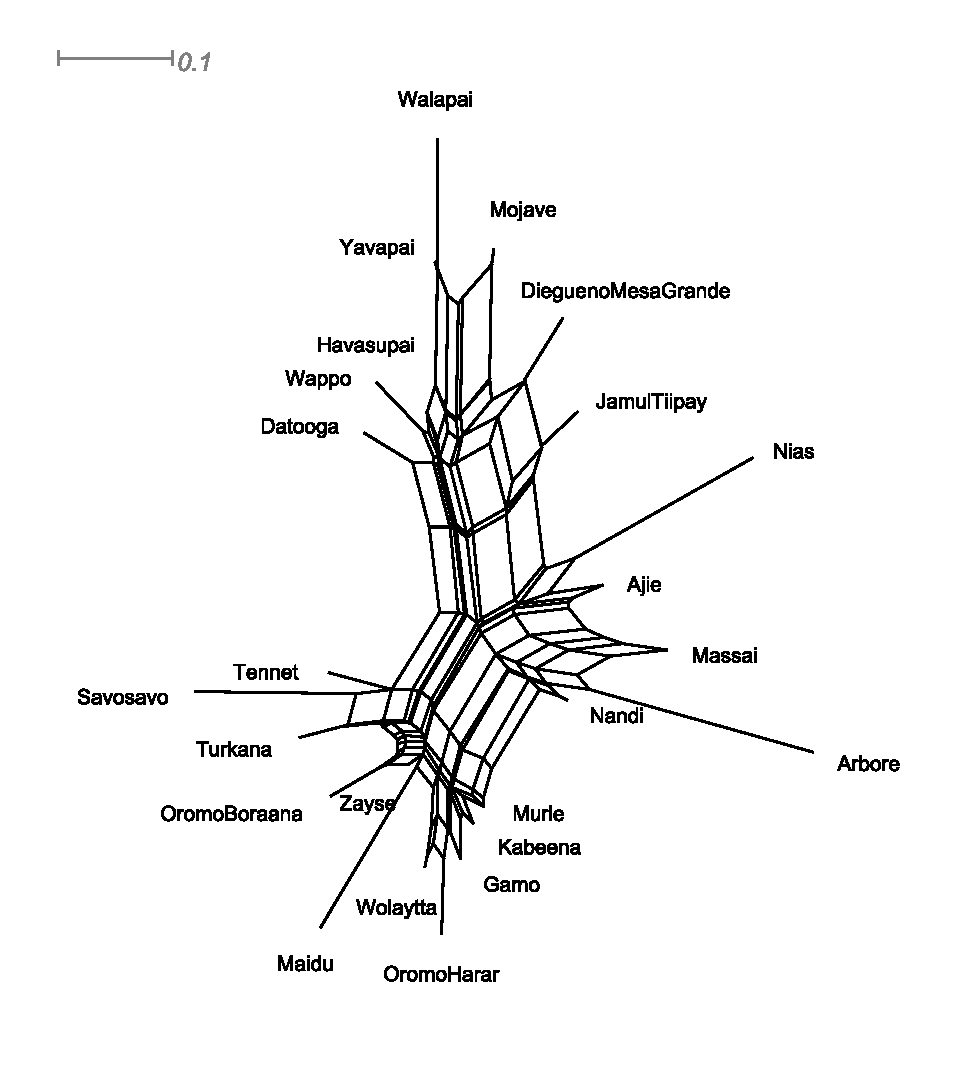
\includegraphics{languages}%
}}%
\caption{Similarity network of the languages studied}\label{NetLang}
\end{figure}
The most salient subdivision of the language network is the one between the Yuman languages and Wappo\il{Wappo}, which form a North-West American subtype of marked"=S, and the rest of the network. 
The other American language of this sample, i.e. Maidu\il{Maidu}, does not belong to this typological subgrouping. 
The Nilotic language Datooga also appears to be more similar in type to the American languages than to any other language in the sample. 
Also, the groupings within the Yuman genus are quite accurately mirrored by the network. Mesa Gande Diegue\~no\il{Diegue\~no (Mesa Grande)} and Jamul\il{Jamul Tiipay} Tiipay both belong to the Delta-California branch of Yuman, while Yavapai\il{Yavapai}, Walapai\il{Walapai} and Havasupai\il{Havasupai} form the Arizona Pai branch. 
Mojave\il{Mojave}, which is located between these two groups in the network, belongs to the River Yuman branch. 
Other genealogical groupings that are represented in the network are the Afro-Asiatic languages from the Omotic and Eastern Cushitic branch (except Arbore\il{Arbore}, which is separated from its related languages).
Even though these languages are found in an continuous segment of the network (with intervening Maidu\il{Maidu}, which exhibits the most areally atypical pattern of the sample), they do not form a clear branch structure that would set them off from other languages. 
However, there is a distinct African subgroup, although it is not limited to the languages of the Afro-Asiatic family. 
If one adds the non-related Surmic languages (Murle\il{Murle} and Tennet\il{Tennet}) and the Nilotic language Turkana\il{Turkana} of the Nilo-Saharan family as well as Maidu\il{Maidu} and Savosavo\il{Savosavo}, a distinct group separated from the remaining languages by a branch-like structure can be identified. 

The Austronesian languages Aji\"e\il{Aji\"e} and Nias\il{Nias} are located in adjacent position at the border between the North American and African languages, but like the Afro-Asiatic language, they do not form an individual branch structure.
The Nilotic languages, on the other hand, are scattered all over the network and so do not form any continuous subsection of the network.
This genus has already been shown to be the most divergent at the tabular ranking in the previous section.


Finally the data is grouped by genus (Figure~\vref{NetGenus}). 
\begin{figure}[h,t,b,p] \centering \resizebox{\textwidth}{!}{\fbox{%
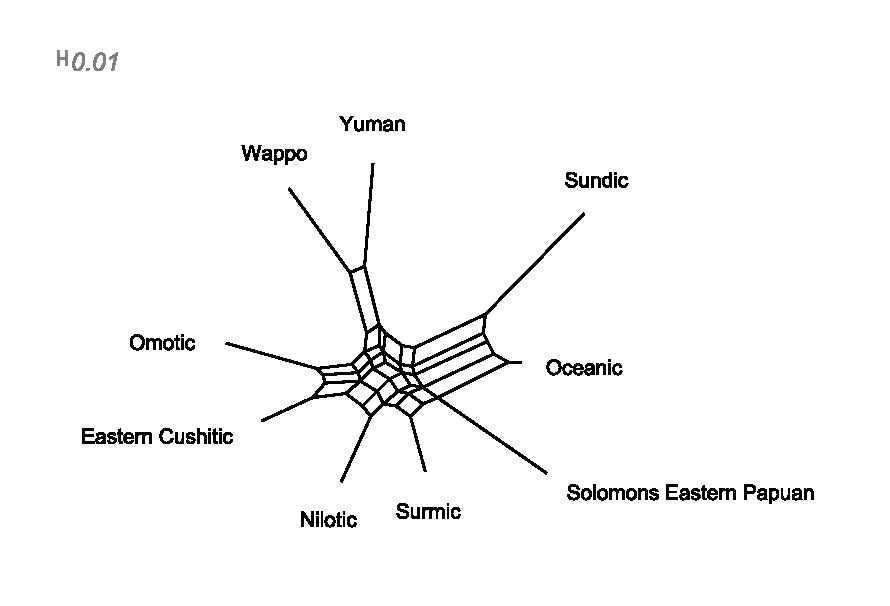
\includegraphics{genus}%
}}%
\caption{Similarity network of the genera studied}\label{NetGenus}
\end{figure}
For this network, Maidu\il{Maidu} (Maidu\il{Maidu}an) has been eliminated.
It has already been noted that Maidu\il{Maidu} behaves quite unusual compared with the marked"=S languages in its macro-area.
Also compared with the total set of marked"=S languages, it stands out by employing the S-case almost like would be expected from a regular nominative"=accusative language. 
Other than the Omotic marked"=S languages, which also make wide use of the S-case, and which have overtly coded forms for both S-case and zero-case, on the formal level Maidu\il{Maidu} is a typical marked"=S language. 
\enlargethispage{\baselineskip}

Also\is{multidimensional scaling|(} when analyzing the language-internal grouping of uses in the Maidu\il{Maidu} data, the picture is confusing. 
The semantic map in Figure~\vref{maidu} visualizes the use of S-case (red/subj), zero-case
(blue/zero) and other case-forms (black/other) in Maidu\il{Maidu}.\footnote{Again, I have to thank
  Michael Cysouw. This time for producing and sharing this semantic map.}  
\begin{figure}[h,t,b] \centering \fbox{%
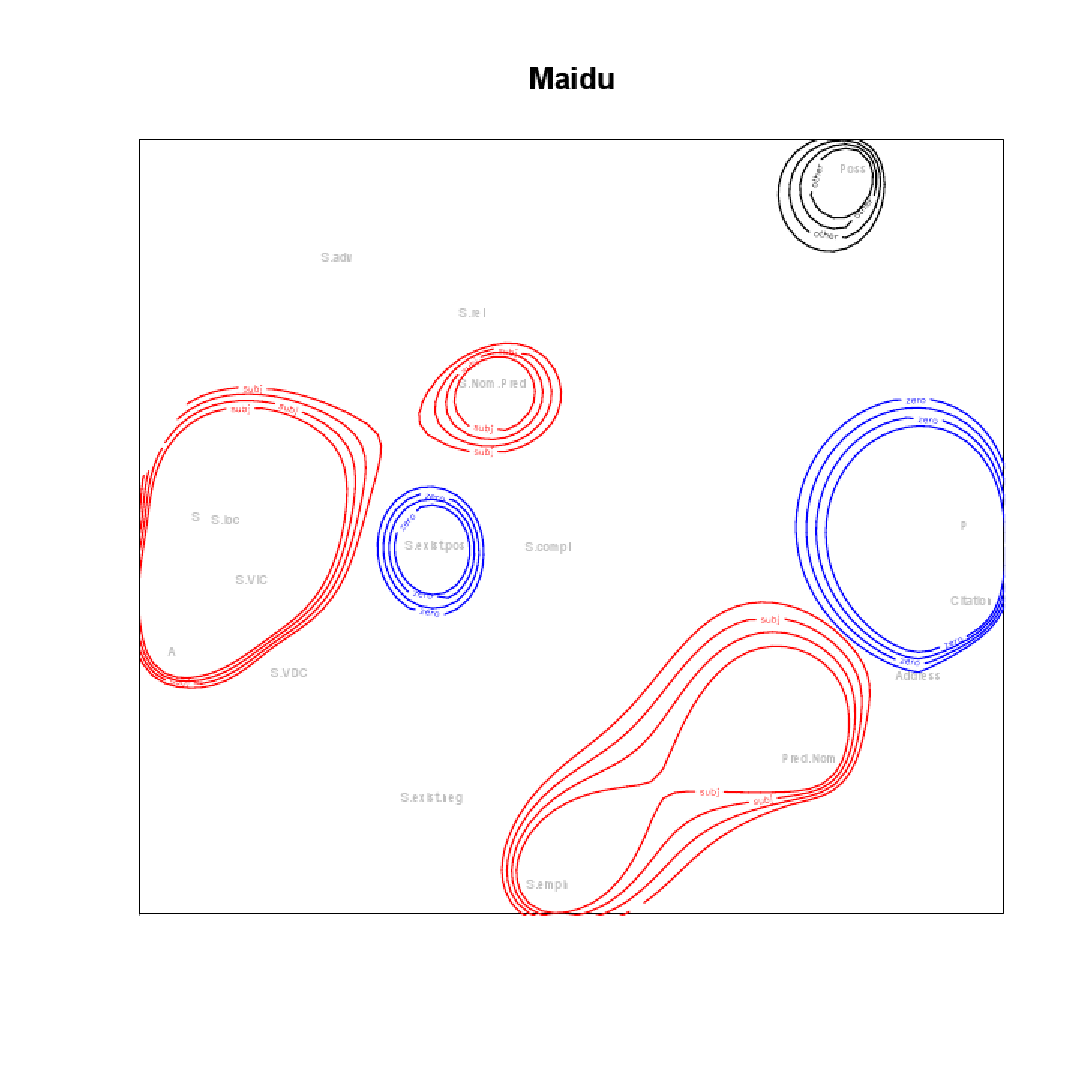
\includegraphics[scale=.65]{maidu}%
}%
\caption{Maidu semantic map (MDS)}\label{maidu}
\end{figure}
The arrangement of the roles is derived from the usage of these case-forms for the individual roles across all languages of the sample via multidimensional scaling (MDS). 
Semantic maps derived through MDS and how they can be used to analyze and understand the nature of linguistic meanings are discussed by \citet{Cysouw:2010}.
While the other languages use the individual case-forms for continuous parts of the semantic map (or at least only one case-form shows discontinuous usage), Maidu\il{Maidu} rather constitutes a semantic patchwork.\is{multidimensional scaling|)}  

Furthermore, including Maidu\il{Maidu} into the genus level network gives no clear picture. 
If one excludes this data, the genealogical and areal groupings come out quite nicely, as demonstrated in Figure~\ref{NetGenus}.
The North American languages have already formed a distinct subgroup on the language level. 
Not surprisingly, Yuman and Wappo\il{Wappo} also form the most clear subgrouping in this graph. 
They branch off almost tree-like from the other genera. 
The African genera also form a distinct area of the network, and especially the Afro-Asiatic genera Omotic and Eastern Cushitic even form a small separate branch. 
The two Nilo-Saharan genera, Nilotic and Surmic, are adjacent to one another, though they form no branch-like structure. 
The Austronesian genera, Sundic and Oceanic, also from a separate branch of the network (though the branching is not particularly strong) with Solomons East Papuan, the other Pacific genus, in adjacent position.\is{phylogenetic networks|)}



\section{Geographical patterns}\label{area}\is{typology!areal|(}

It has been noted several times in this study that the distribution of marked"=S languages is highly skewed in terms of geography.
\enlargethispage{\baselineskip}
North-East Africa, where the pattern is found in both the Afro-Asiatic and Nilo-Saharan family, appears to be a breeding ground for languages of this type. 
Another area in which marked"=S languages appear frequently (as compared with the overall distribution over the world) is the lower North American Pacific coast. 
The majority of marked"=S languages found in this region are closely-related with one another as they belong to one genus (i.e. Yuman). 
However, two unrelated marked"=S languages, namely Wappo\il{Wappo} and Maidu\il{Maidu}, do occur in the same macro-area.
Finally the Pacific macro-area is home to some languages of the marked"=S type.
The three Pacific languages with the most prominent marked"=S pattern are stretched out over a quite large area. 
However, if additionally to Nias\il{Nias}, Aji\"e\il{Aji\"e} and Savosavo\il{Savosavo} the less prototypical marked"=S languages of the same region are included, such as the ones discussed in Chapter~\ref{exposed}, the Pacific exhibits an above-average concentration of marked"=S languages as well. 
%\enlargethispage{\baselineskip}
In this section, I will take a closer look at the areal patterings of marked"=S languages.

\begin{figure}[h,t,b] \centering \resizebox{\textwidth}{!}{\fbox{%
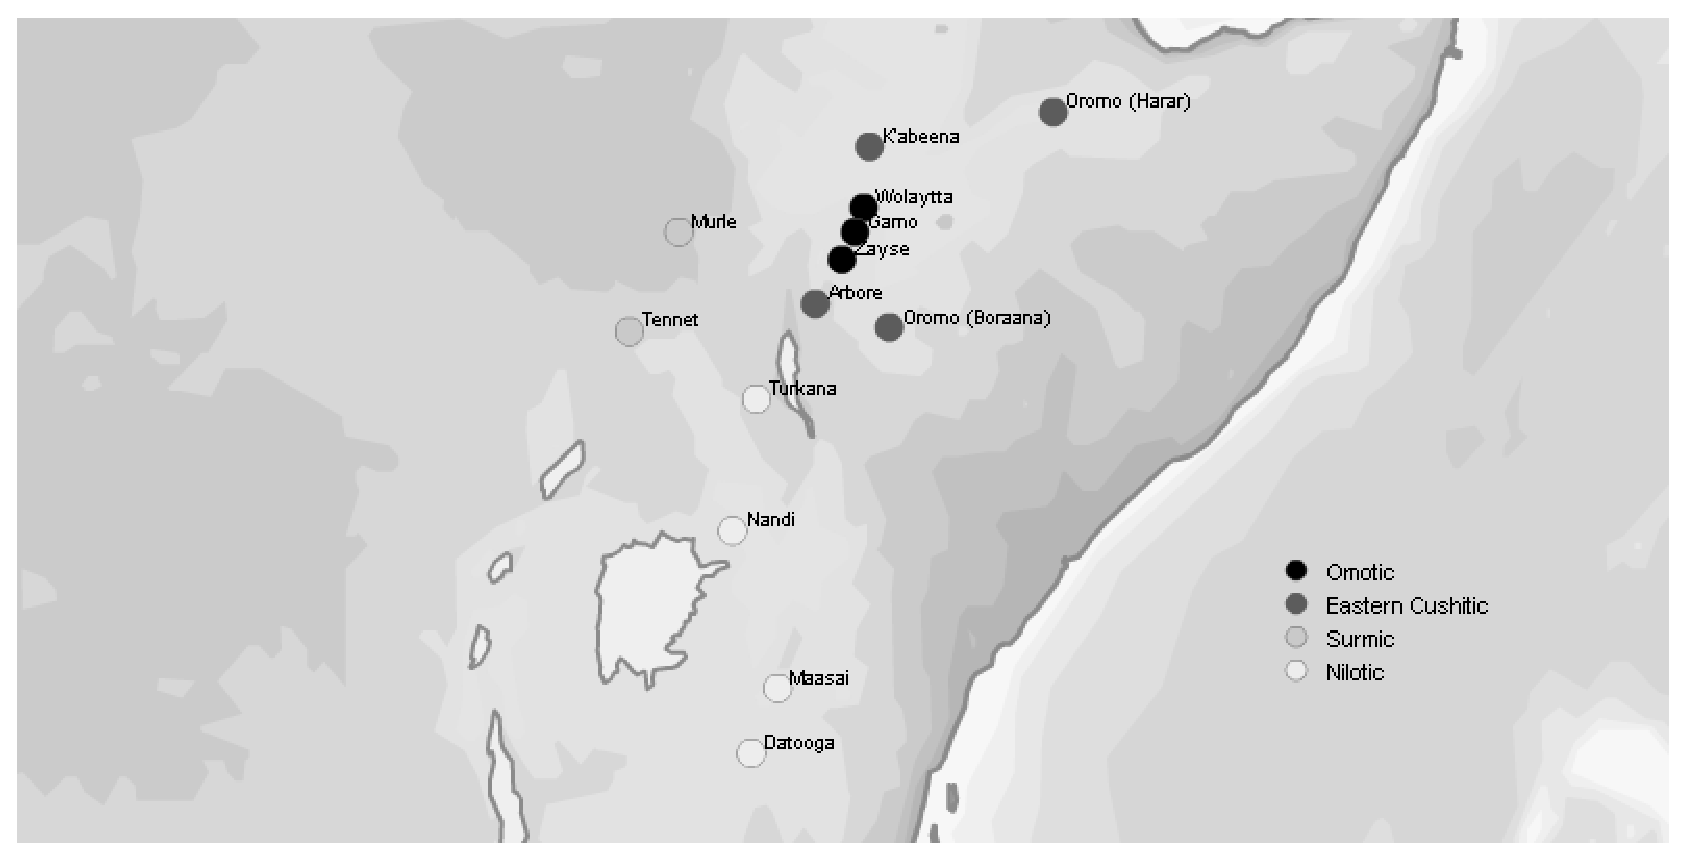
\includegraphics[scale=0.44]{MapAfrica}%
}}%
\caption{Marked"=S languages of East Africa by genus}\label{MapAfrica}
\end{figure}

The largest number of languages in my sample is found in North-East Africa. 
In addition to the large number for the African marked"=S languages, they also exhibit genealogical diversity as they are represented by four distinct genera belonging to the Afro-Asiatic (Omotic and Cushitic) and Nilo-Saharan (Surmic and Nilotic) families (cf. Figure~\vref{MapAfrica}).\footnote{The language Maa\il{Maa} is represented with its alternative name Maasai in the map.} 
Marked"=S patterns have been reported from other genera of this area, but the data available for them was not suitable to include in this study. 
Areal influence is often proposed as an explanation if a certain linguistic pattern is found in a group of geographically adjacent but non-related languages, even more so if the respective pattern is rare on a world-wide basis.
The locus of the African marked"=S languages has been suggested as a linguistic area on several occasions.
\citet{Gueldemann:2005}\is{typology!areal!Ethiopian language area|(} describes a pattern of forming complex predicates through a special type of auxiliary that is uniquely found in the region referred to as Chad-Ethiopia macro-area. 
This region has been described as a linguistic area in earlier work by \citet{Greenberg:1983}, \citet{Ferguson:1976} and \citet{Heine:1976}, though the name and exact boundaries of the supposed area differ between the authors.
However, the existence of an `Ethiopian language area' is disputed by \citet{Tosco:2000}. 
Yet, his main argument is not that there has not been linguistic contact between unrelated languages in this area, but that the influence has been unidirectional. 
He lists multi-directional influence and divergence towards a common model as defining criteria for linguistic areas.\is{typology!areal!Ethiopian language area|)} 
The network in Figure~\ref{NetLang} has shown that the African languages do not group according to their genealogical affiliations in most cases with respect to the roles studied here. 
Only the Omotic languages in combination with most Cushitic languages do occur in adjacent position. 
However, they do not exhibit any clear tree-like branching from the other African languages (and also the Pacific languages plus Maidu\il{Maidu}). %THis might change
Instead they all are of the same general type, with the exclusion of Datooga, which is more similar to the North American languages in its behavior. 
Notably Datooga, which is the least typical African marked"=S language, is spoken at the periphery of the geographical region these languages cover.
In addition, Datooga and Maa\il{Maa} are the two African languages that make the widest use of the zero-case and thus have been shown to behave quite differently than the two other Nilotic languages in the sample in Table~\ref{SumRoleLang}. 
Indeed, Maa\il{Maa} is the language that is spoken closest to Datooga, though it is not the language which is related most closely in terms of genealogy. 


\begin{figure}[h,t,b] \centering \resizebox{\textwidth}{!}{\fbox{%
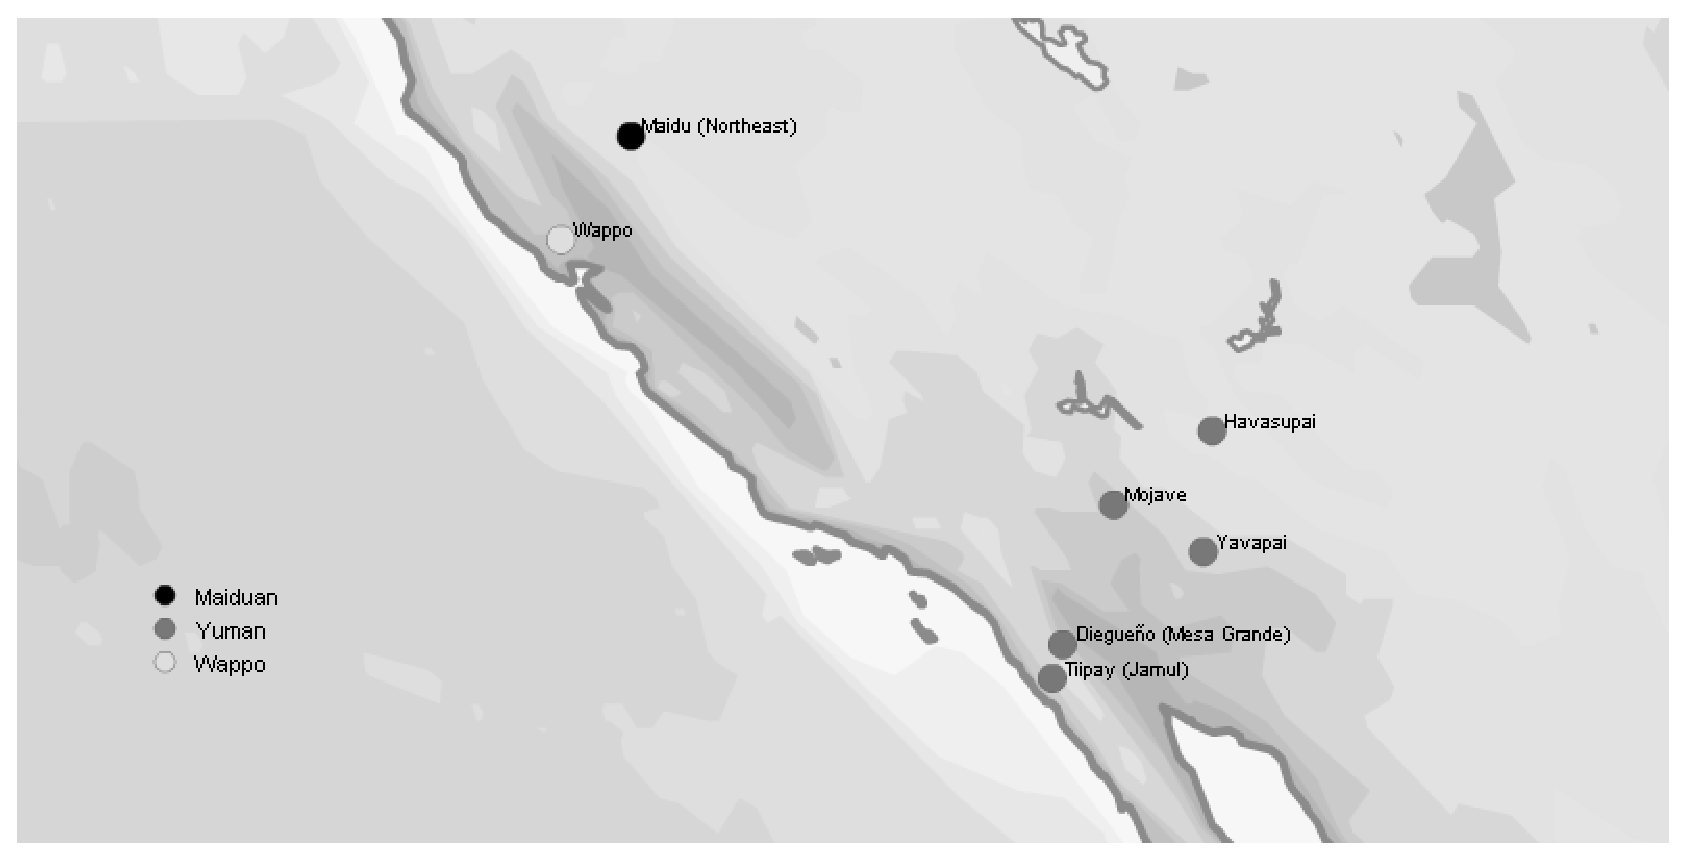
\includegraphics[scale=0.44]{MapNA}}%
}\caption{Marked"=S languages of North-West America by genus}\label{MapNA}
\end{figure}

The second larger grouping of marked"=S languages is found in North-West America. 
These languages are far less genealogically diverse than their African counterparts. 
The majority of languages belongs to the Yuman genus, which is completely of the marked"=S type, except for only one language, namely Kiliwa \citep{Mixco:1965}, which is also seen as the language that first branched of within the genus \citep{Joel:1998}. %find better source
Apart from the Yuman languages, two other marked"=S languages of this region are studied here. 
Wappo\il{Wappo} and Maidu\il{Maidu} are both located quite a stretch to the North from the Yuman languages (cf. Figure~\vref{MapNA}), so that the American languages do not form a contiguous area.
Apart from the close geographical distance between Maidu\il{Maidu} and Wappo\il{Wappo}, these two languages do not show a similar linguistic behavior. 
Wappo\il{Wappo} rather conforms to the most frequent type of American marked"=S languages with the Yuman languages. 
Maidu\il{Maidu} does not show any similarities to this type.
In the network in Figure~\ref{NetLang}, it is located somewhere between Omotic and some Cushitic languages, the main similarity to which is Maidu\il{Maidu}'s equally high percentage of S-case use.
For the Yuman languages of North America, genealogy is probably the main factor behind their common typological profile with respect to their marked"=S case-system.
Wappo\il{Wappo} is a language of the same greater area which is not related to this genus. 
However, it has a typological profile similar to the Yuman languages.
No contact history between the Yuman languages and Wappo\il{Wappo} is known and the geographical distance between the languages (in addition to the large number of intervening languages) makes this scenario not very likely. 
However, one should not rule out that in prehistoric times both Wappo\il{Wappo} and the Yuman languages were part of a larger linguistic area in which marked"=S languages were more abundant. 
If one takes this scenario seriously, Maidu\il{Maidu}, which is located more closely to Wappo\il{Wappo}, could also have been a part of this area. 
Still, Maidu\il{Maidu}'s marked"=S system is distinct from the other North American languages. 
So the system either must have radically changed after the hypothetical period of intense contact with other languages of the marked"=S type, or it could be a development independent of contact with languages that exhibit the typical North American type of marked"=S.

\begin{figure}[h,t,b] \centering \resizebox{\textwidth}{!}{\fbox{%
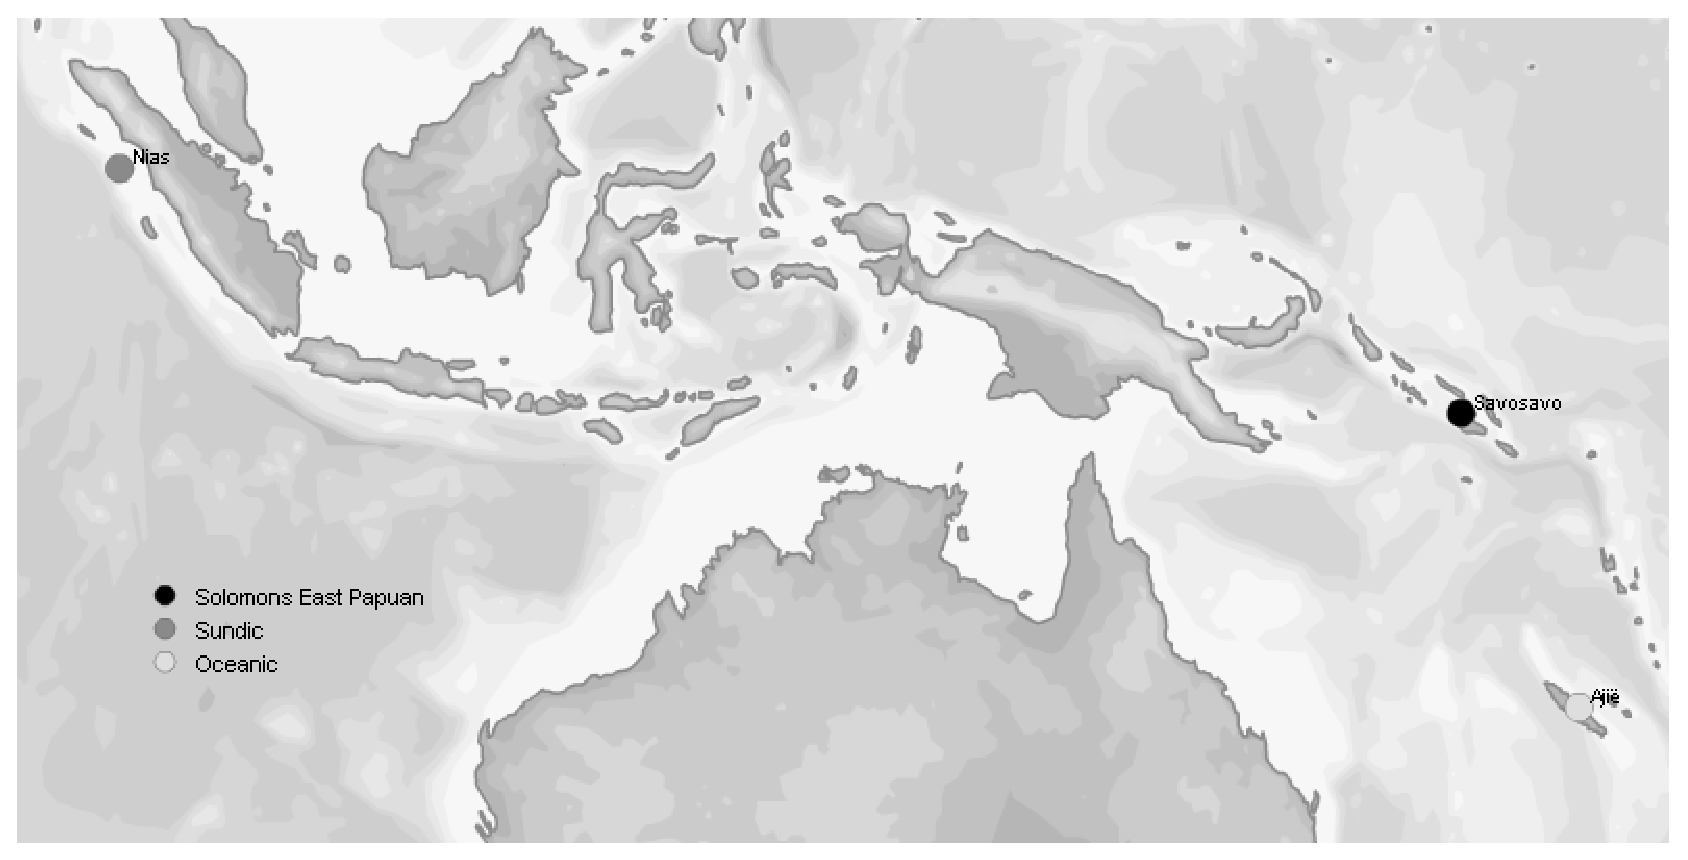
\includegraphics[scale=0.44]{MapPac}%
}}\caption{Marked"=S languages of the Pacific by genus}\label{MapPac}
\end{figure}

Finally, the sample included three marked"=S languages from the larger Pacific region. 
%\enlargethispage{\baselineskip}
Comparing their distribution (cf. Figure~\ref{MapPac}), it becomes clear that arguing for contact between these languages as source for the marked"=S pattern would be rather difficult given that these three languages are stretched out from the West Coast of Sumatra to the Solomon Islands and down to New Caledonia. 
In addition, the genealogical relation between these languages is very distant (Nias\il{Nias} and Aji\"e\il{Aji\"e} belong to different genera of the Austronesian family) or non-existent (as between Savosavo\il{Savosavo} and the other two languages). 
In between the three languages studied in detail lies the entire Indonesian Archipelago including all of Papua as well as large stretches of the Pacific Ocean.
However, within this area there are a number of languages exhibiting a pattern that resembles the marked"=S languages in some respect. 
I have discussed this pattern, which consists of overt subject-marking only in certain, mostly emphatic\is{emphatic subject}, contexts, in Chapter~\ref{emphaticS}.
Adding these languages to the map, as done in Figure~\ref{MapPacAll}, at least the Eastern half of the region pictured here gets closer resemblance to an geographically contiguous area, which includes Savosavo\il{Savosavo} and Aji\"e\il{Aji\"e} at its periphery. 

\begin{figure}[h,t,b] \centering \resizebox{\textwidth}{!}{\fbox{%
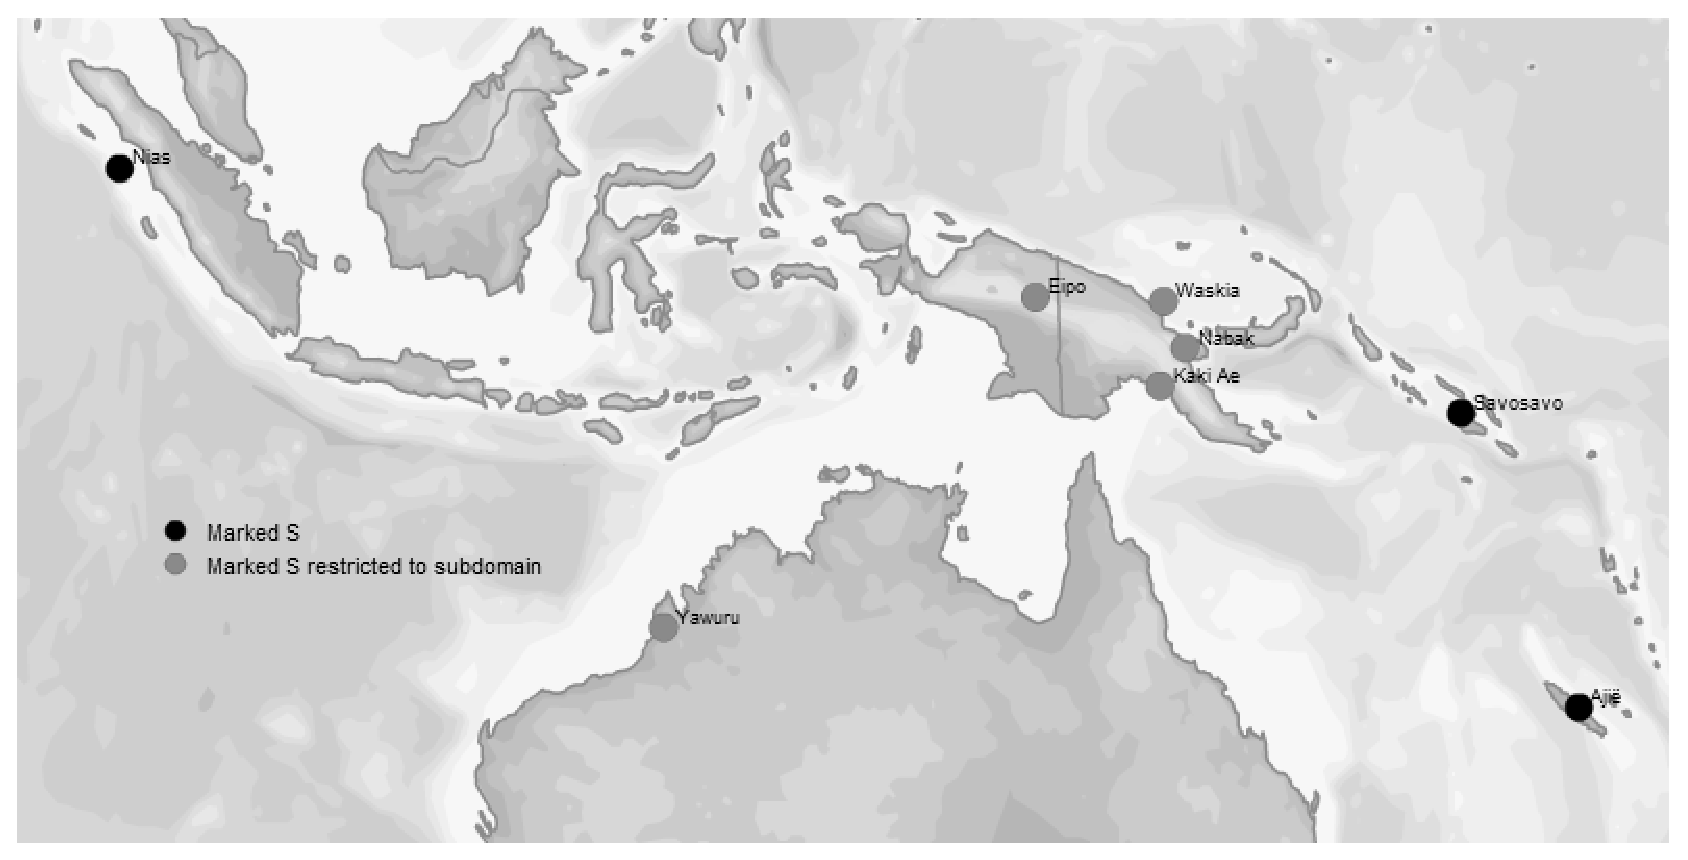
\includegraphics[scale=0.44]{MapPacAll}}%
}\caption{Marked"=S languages of the Pacific including full and restricted patterns}\label{MapPacAll}
\end{figure}\is{typology!areal|)}


\section{Summary}\label{sumtyp}

In this chapter, I have presented a summary of the data gathered through Chapters~\ref{nompred}--\ref{extrasyn}. 
The micro-alignment approach I have chosen for the investigation of marked"=S languages consists of collecting data on the case-marking patterns for a number of roles. 
These roles were selected from several contexts that include a subject-like\is{grammatical relations|subject} role (such as nominal predications or existentials\is{existential predication}), or roles that are commonly associated with the so-called `unmarked case' of standard nominative"=accusative and ergative"=absolutive languages (i.e. the nominative or absolutive respectively).
The data collected on the case-marking of these roles have been analyzed from two perspectives: from the point of view of these roles and the point of view of the languages studied.

I have demonstrated that the encoding of the roles chosen for this micro-ty\-po\-lo\-gy of the marked"=S coding-system range from (almost) exclusive encoding with the S-case to zero-coding in almost all instances. 
Roles that do not constitute any type of subject, though they have been associated with the nominative case in previous work, are especially likely to be zero-coded. 
These roles are the citation\is{citation form} form and predicate nominals\is{nominal predication!predicate nominal}, as well as attributive\is{possession!attributive} possessors and terms of address\is{terms of address}. 
The latter two are, however, also frequently encoded through other overt non-S-case case-forms.

Variation is not only found between the different roles but also between the marked"=S languages. 
While some make strong use of the zero-case, others use this form more sparsely. 
Especially the Omotic languages and Maidu\il{Maidu} do not differ strongly from standard nominative"=accusative languages in the use of the S-case. 
On the other end of the hierarchy, there are the distantly related Austronesian languages Aji\"e\il{Aji\"e} and Nias\il{Nias}, a number of the North American Yuman languages and Wappo\il{Wappo} as well as the Nilotic languages Datooga and Maa\il{Maa}. 
These languages make especially wide use of the zero-case and also employ it for some types of subjects. 

Given the rarity of the phenomenon, this study has included as many languages as possible and no quotas have been set in advance, e.g. one language per genus (or other pre-defined grouping). 
In this section, in addition to the data set including the individual languages, a controlled version in which only one data point per genus was included for each role has also been presented. 
The differences between the two sets of data, the language and genus level, have been very small. 

Also, two different encodings for the case-marking have been employed for the data. 
These two codings roughly correspond to the weak and strong interpretation of K\"onig's (\citeyear{Koenig:2006}) functional marked"=S hypothesis. 
The weak version states that the zero-case should be employed in more contexts in marked"=S languages than the overtly coded S-case. 
To analyze this version of the hypothesis the data has been coded according to whether a role is marked with the zero-case, S-case or another case-form. 
The strong version of the hypothesis states that the zero-case should be more frequent than any other type of encoding, respectively the data has been coded as zero-coding and overt coding to test this claim.
The differences between the two types of coding have been minor and are mostly restricted to non-subject roles such as attributive\is{possession!attributive} possessors.
Most languages either choose the zero-case or the S-case for the majority of roles investigated in this study.

In addition, the data have been analyzed in form of phylogenetic networks produced through the NeighborNet algorithm. 
The networks in general confirm the picture gained from the depiction in the form of tables ranked by percentage of use of the individual case-forms.
The roles appear to show a clear separation between those that constitute some kind of subject and those that have different, mostly non-clause level, functions. 
The data on the languages do not show any neat subtypes of marked"=S languages apart from the grouping of the Yuman languages and Wappo\il{Wappo}.
The data on the genus level, meanwhile, produced an accurate picture of the genealogical and areal groupings of languages. 
However, one language, namely Maidu\il{Maidu}, had to be excluded in order to arrive at this neat depiction. 

Geographically, the languages of the sample can bee grouped as belonging to three marco-areas: North-Eastern Africa, the North American West Coast, and the Pacific. 
The languages of North America, to the exclusion of Maidu\il{Maidu}, do form the most distinct subtype in all analyses of the data. These languages mostly belong to the Yuman genus. 
However, non-related Wappo\il{Wappo} also behaves quite similarly to the Yuman languages. The other type of marked"=S languages against which the American type can be set off consists mostly of the African languages. 
The Afro-Asiatic languages, especially of the Omotic genus, are another potential subtype of marked"=S languages. 
However, these languages do not form as distinct a subtype branching off from other languages as does the American type. 
Nilo-Saharan, the other African language family, generally tends to cluster around the Afro-Asiatic languages. 
These languages do not provide a legitimate grouping with each other, especially the languages of the Nilotic genus do not exhibit a uniform behavior according to the methods of comparison employed. 
Languages of the Pacific are too few within the sample to make any strong claims about a distinct type. 
Yet, the two Austronesian languages Aji\"e\il{Aji\"e} and Nias\il{Nias} behave quite similarly to one another in the different modes of analysis used in this chapter.  



\chapter{Conclusion}\label{conclusion}

%\setcounter{exx}{0}

\section{Summary of the findings}

In this study, I have analyzed the micro-alignment of a number of marked"=S languages.
Marked"=S languages exhibit a peculiar pattern of encoding the basic (in-) transitive roles S, A and P in that they overtly mark the S relation of intransitive verbs while using a non-overtly coded form of a noun for one of the arguments of transitive verbs (for more details cf. the definition and examples of marked"=S languages in Section~\ref{definition}). 
In addition to the S, A and P roles, this study has investigated the coding of a number of additional S-like roles.
The additional roles have been selected from the contexts defined in Chapter~\ref{method}.
While some of these roles behaved like regular overtly-marked intransitive S arguments in most languages, others were almost exclusively encoded by the zero-coded case-form. 
Figure~\ref{SumRole} summarizes  the results of the previous chapter, in which the different contexts have been compared with one another.
The roles have been ordered with respect to their likeliness to be encoded in the same way as intransitive S arguments in the languages of the sample. 
The further to the top a role is located, the more often it is encoded with the S-case.
Roles that are represented next to each other in Figure~\ref{SumRole} exhibit almost identical behavior in this respect.
These preferences are quite stable between different calculations, both when including all individual languages on which enough data was available (without employing any mechanisms of genealogical and/or areal control) and when the data were normalized to include only one data point per genus.

\begin{figure}[ht] \centering \fbox{
\begin{picture}(285,280)

\put(100,255){\makebox(70,20){intransitive S}}
\put(100,230){\makebox(70,20){locational S}}
%\put(155,230){\makebox(70,20){S of VIC}}
\put(45,205){\makebox(70,20){S of positive existential}}
\put(155,205){\makebox(70,20){S of VDC}}
\put(100,180){\makebox(70,20){S of adverbial clause}}
\put(100,155){\makebox(70,20){S of nominal predication}}
\put(100,130){\makebox(70,20){S of negative existential}}
\put(155,105){\makebox(70,20){S of relative clause}}
\put(45,105){\makebox(70,20){emphatic S}}
\put(100,80){\makebox(70,20){S of complement clause}}
\put(100,55){\makebox(70,20){predicate nominal}}
\put(45,30){\makebox(70,20){attributive possessor}}
\put(155,30){\makebox(70,20){term of address}}
\put(100,5){\makebox(70,20){citation form}}

\put(260,20){\line(0,1){250}}
\put(270,20){\line(0,1){250}}
\put(260,270){\line(1,0){10}}

\put(255,20){\line(1,0){5}}
\put(270,20){\line(1,0){5}}

\put(265,10){\line(1,1){10}}
\put(265,10){\line(-1,1){10}}

\end{picture}}

\caption{Coding of S-like roles in marked"=S languages (ordered from most S-like to least S-like)}\label{SumRole}
\end{figure}


%In addition the individual languages and genera have been compared with respect to their frequency of employing a certain case-form for a given role. In all cases two different encoding-patterns have been used for the data. The data has either been analyzed as coding via the zero-case, the S-case or an other overt case-form, or a two-way distinction between overtly coded forms and zero-coded forms has been made. The data have been rather stable between these two types of encoding as well, differences in pattering between the two encodings have only been found for a minority of roles and languages.
Two different methods of analysis, first through a ranking by percentage and second through the more sophisticated NeighborNet algorithm, have revealed a similar pattern for the different roles, namely, a gradual shift from coding via S-case to coding via zero-case. 
The subject-like roles, especially subjects of locational clauses, being the one extreme and extra-syntactic roles, especially the citation form of a noun, being the other.
%On language level the two methods have as well led to similar results. 

Apart from distinguishing which roles behave most or least like intransitive S arguments in their encoding, the similarities and differences between the individual languages have also been evaluated. 
There is a clear subtype of marked"=S languages to which most marked"=S languages of North America belong (excluding only Maidu\il{Maidu}). 
Further, there is an African type of marked"=S comprising the Afro-Asiatic languages of the Omotic and East Cushitic genera as well as Surmic. 
The Nilotic languages do not behave in a consistent pattern that would allow to classify them as following one or the other pattern. 
Languages of the Pacific exhibit some similarities, but the data does not justify proposing a distinct subtype of marked"=S for them.% probably due to the small number of languages in the overall sample. 

After this brief summary of the results, I will now discuss the implications of these findings for the understanding of marked"=S languages.
The central motivation of this study has been to test whether the unexpectedness of the marked"=S coding-pattern based on the purely formal aspects of the system can be adequately explained in terms of functional motivations, as it has been proposed in \citet{Koenig:2006}. 
This major question will be addressed in Section~\ref{discussion}. While an important factor in understanding marked"=S languages, the range of functions a case-form has cannot be the sole explanation for their existence. 
Furthermore, to allow for meaningful generalizations over the functions of marked and unmarked case-forms, one needs to apply a consistent definition of markedness that is independent of functional considerations.
Further, I will review the micro-alignment approach that I have used for this investigation and comment on its usefulness and limitations in Section~\ref{methodcomments}.
I also pointed out in the introductory chapter (Section~\ref{theoretical}) that marked"=S languages are a serious challenge for some of the more formalistic approaches to alignment and case-assignment in particular. 
I will take up this discussion in Section~\ref{consequencesformal} and comment on the possibilities of integrating the finding on marked"=S languages into these formal approaches. 
Finally, I will address some questions that remain open or have been raised by the findings of this study, and which should be targeted in future research (Section~\ref{furtherresearch}).  

\section{Generalizations about the functional motivations for marked"=S languages}\label{discussion}\is{marked-S languages!functional definition|(}

Marked"=S languages have caught the attention of linguists based on a strictly formal criterion, namely the overt marking of the S argument found with these languages. 
The unexpectedness of the marked"=S system is for example expressed as Universal 38 in \citet[75]{Greenberg:1963}.
The two points of view from which the existence of this unusual case-systems have been considered are  the historical development of these systems and their functionally-based motivations. Of course, these two points of view do not have to be mutually exclusive. Historical changes in the grammar of a language can certainly have a functional motivation; some linguists will even argue that they must have one. 
In contrast to the formal definition, a functional definition of marked"=S languages has also been
proposed \citep{Koenig:2006}.%
\enlargethispage{\baselineskip}
In this definition, the functional range of individual case-forms is the central criterion for the `markedness' or `unmarkedness' ascribed to each case-form.
The functional aspect, i.e. the number of functions covered by the case-forms, is an important aspect in the study of marked"=S languages.  
 However, the number of roles covered by either zero-case or S-case does vary considerably between the languages studied here.\footnote{As defined in Section~\ref{label} the term S-case is employed for the case-form that covers the function of encoding transitive S arguments (i.e. the nominative in nominative"=accusative languages and the absolutive in ergative"=absolutive languages). The term zero-case refers to the case-form that is used for the non-S-case-marked argument of transitive verbs, and that is zero-coded in marked"=S languages (i.e. the accusative in nominative"=accusative languages and the ergative\is{case!individual forms!ergative} in ergative"=absolutive languages).}

For some languages the existence of marked"=S coding cannot be plausibly argued for based on functional motivations of this type.
From the point of view of the formal encoding of case-forms, the Californian language Maidu\il{Maidu} is a regular marked"=S language with an overt Nominative case-marker and a zero-coded Accusative. 
Yet, the range of functions that the zero-coded Accusative covers does not extend far beyond the encoding of transitive P arguments. 
Maidu\il{Maidu} is, however, not the only problematic case for the functional account of marked"=S languages. 
The languages that are identified as being of the marked"=S type by a functional rather than purely formal definition, i.e. the languages referred to as Type 2 marked"=nominative languages by \citet[658]{Koenig:2006}, do not use the `zero-coded' form for as many of the roles as the languages meeting the strict form-based definition do.  
For the Type 2 marked"=nominative languages, the function of the accusative case as citation form (and in other extra-syntactic contexts) is taken as the main argument to consider this form as being the more basic form. 
Based on the data collected in this study, the use as a citation form is also the main function of the zero-coded form after its use as the case-form of transitive P arguments, while the Type 2 languages do not extend its use to more subject-like roles.

Taking a radically economical approach to case-marking, one could propose the following explanation. 
If two case-forms of a noun do differ in the number of segments they consist of, the form that has the smaller number of segments will be preferred because of its lower production effort. 
If the two case-forms consist of the same amount of segments, no such pressure exists to choose one form over the other. 
Linguistic explanations that propose such radically economy-based argumentations can be criticized on various grounds. 
One argument against this approach would be that actual ease of articulation rather than the bare number of segments is a stronger factor. 
Extra segments added to a form, such as final vowels, can lead  to a less complex syllable structure and thus increase the ease of articulation. 
Consequently this entire discussion returns to the initial question of how one defines the concept of linguistic markedness, which I discussed in Section~\ref{markedness}. 
Since different definitions of markedness can result in different identification of marked versus unmarked forms in individual languages, there is always the possibility of choosing the definition that best fits one's analysis of any language (e.g. defining the `marked' form as the one with the more marked syllable structure even though this might be the morphologically zero-coded form). 
While this approach improves the consistency of an analysis on a per-language level, comparability between languages and consequently cross-linguistic generalizations over marked"=S coding are rendered meaningless, since this leads to a circular definition of the marked"=S system. 
If one chooses the definition of marked versus unmarked case-form which best fits the prediction that the unmarked form is used in more contexts, then it necessarily follows that the unmarked form is made a wider use of in marked"=S languages.\is{marked-S languages!functional definition|)} 

\section{Concluding remarks on the micro-alignment approach}\label{methodcomments}\is{micro-alignment approach|(}

As Chapter~\ref{typology} has shown, languages belonging to the marked"=S coding type behave quite differently in terms of micro-alignment structures. 
While the pattern of marking the S, A and P functions of prototypical verbs employs the same pattern of case-marking in these languages, the marking of other types of clauses differs strongly between the languages. 
Differences in encoding between different clause-types or based on other factors, like the ones discussed in Section~\ref{grammar-based} are also known from languages with other coding-systems. 
Still, coarse classifications of language as being of the nominative"=accusative or ergative"=absolutive type are made frequent use of in linguistic studies.
Since much of the debate on marked"=S languages focuses on overt coding properties (and the unexpectedness of this pattern), an in-depth investigation of the coding-patterns of more than just the most basic clauses is necessary to fully understand this unusual pattern.  

The contexts and roles chosen in this study have been defined based on the variation that the languages studied here exhibited. 
Data for all languages was basically gathered in a parallel fashion and not one language after the other, since the study of one language potentially revealed a new pattern of variation that could profitably be included in the study. 
On the other hand, based on an initial list of possibly interesting domains of grammar, data have been collected on roles that did not show any interesting patterns in any or almost any languages of the sample and have thus not been presented in the final study. 

A small drawback of this approach is the frequent omission of parts of the grammar in the description of languages that do not exhibit any variation in the respective domain.\footnote{The same is, however, true for most comparative work that is carried out through available descriptions of languages.} 
Negative evidence, especially when dealing with a very limited set of examples as data base, cannot be taken as evidence of the absence of a certain pattern in a given languages. 
This has led to a considerable number of missing data points. Consequently, the respective percentage of languages that deviate from the pattern conceived as the norm, i.e. S-case-marking on subject-like roles, might be a little too high in the figures presented in Chapter~\ref{typology}. 
This is based on the assumption that if a grammar does not discuss a given context, there will more likely be no variation from the standard pattern in this domain.
In addition, the larger the number of languages studied, the larger the number of contexts of interest will become with this approach. 
Consequently, when relying largely on secondary data, the larger the number of missing data points will become. 

Given these limitations, the micro-alignment approach -- however, this is true for any approach that aims at including very fine-grained distinctions on any domain of grammar -- is best employed in more detailed studies operating samples of a smaller size. 
Preferably, primary data on the languages studied should be available, which is, however, difficult and tedious to obtain for the majority of the world's languages. 
The approach is less applicable in large scale typological studies aiming at a large number of languages included\is{micro-alignment approach|)}. 

\section{Consequences for formal theories}\label{consequencesformal}

For the languages of the marked"=S type one can identify a case-form that can be analyzed as a default\is{case!default} case, a notion that many formal theories employ.
However, this case-form is not necessarily linked to the form that is used to encode the subject function in a clause. 
For most marked"=S languages, the case-form that should be considered the default\is{case!default} case by factors such as which form is the most basic one in terms of morphological structure (derived forms versus underived forms).
The form which is used in extra-syntactic contexts does coincide with the form used to encode the non-subject argument in basic transitive clauses. 

In Chapter~\ref{introduction}\is{Lexical Decomposition Grammar|(}, I briefly introduced the feature system of Lexical Decomposition Grammar (LDG, \citealp{Wunderlich:1997,Stiebels:2002}). 
In this approach, the default\is{case!default} status, which is ascribed to the nominative or absolutive\is{case!individual forms!absolutive} case, is mirrored through the feature representation of the default\is{case!default} case, which is an empty set. Other cases have non-empty sets of features, and thus are more restricted in their use. 

As argued above for marked"=S languages, one has to assume that the accusative case (or respectively the ergative\is{case!individual forms!ergative} case) functions as the default\is{case!default} case.
If one wants to keep the generalization that the default\is{case!default} case-form should have a feature representation consisting of an empty set of features, and thus being potentially employable in all contexts, one would have to assume that the cases used in marked"=S languages have a different set of features than the  standard feature representations proposed in LDG (cf. Section~\ref{theoretical}).
The following feature representations could be employed:

\begin{itemize}
\item marked"=nominative: [-hr]
\item default accusative: [\quad]
\item marked"=absolutive: [-lr]
\item default Ergative: [\quad]
\end{itemize}

(\ref{theta2}) and (\ref{LDGalternate}) demonstrate the linking of a basic transitive verb using these feature specifications. 
As in in the standard LDG approach, feature specifications for the arguments of a verb are derived from the semantic form and the theta-structure of a verb.
The cases that are available from the lexicon of the language are then matched to the argument positions based on their feature specification, choosing the most concrete case available for each position (\ref{LDGalternate}). 
In marked"=nominative languages, the overtly coded nominative and default\is{case!default} accusative are available. 
Both argument positions could be filled with the default\is{case!default} accusative.
However, the nominative is a better match for the x argument since it is the more concrete case (i.e. it has more features specified) and its feature specification as [-hr] (`there is no higher role') is compatible with the feature specification of this argument position. 
Conversely, in marked"=absolutive languages the two available case-forms, the overtly coded absolutive\is{case!individual forms!absolutive} and default\is{case!default} ergative\is{case!individual forms!ergative}, are matched to the x and y argument position by the same mechanism.  


\begin{exe}\ex\label{theta2}
$ \underbrace{ \lambda \text{x} \quad \lambda \text{y} \quad \lambda \text{s}}_{\text{\normalsize\rm
      theta-structure}}$ \qquad $ \underbrace{\{ \text{see (x,y)} \}
    \text{(s)}}_{\text{\normalsize\rm semantic form}} $ 
\end{exe}

%\pagebreak
\begin{exe}
\ex\label{LDGalternate}
\begin{tabbing}
nominative"=accusative \quad \= \nom{} \quad \= \kill
{}\>$\lambda \text{y}$ \> $\lambda \text{x}$\\
{}\>{+hr} \> {-hr}\\
{}\>{-lr} \> {+lr}\\
marked"=nominative\>\acc{}	\> \nom{}\\
marked"=absolutive\>\abs{} \> \erg{}
\end{tabbing}
\end{exe}

The standard case-representations of LDG only make use of features that have a positive specification. 
In contrast, for the specifications I proposed for the cases of marked"=S languages, negative feature specifications are used. 
This procedure goes against most considerations relevant to the setup of feature systems, in which negative feature specifications are often equated with underspecification with respect to the given feature.
Without doubt, the introduction of the additional cases and their proposed feature specifications would deprive the LDG approach of some of its elegance.
Yet one could argue that this dispreferred feature specification employed to model case-assignment in marked"=S languages is reflected through their cross-linguistic rarity.   
Another possibility, which would not make it necessary to include negative feature specification for the representation of cases would be to introduce a new set of features for languages of the marked"=S type. 
Since this section is not meant as a proposal to reformulate LDG, but rather a sketch of how marked"=S languages could be integrated into that theory, I have restricted myself to employing the features that are already provided by the theory. 

However, there is another issue that makes the inclusion of marked"=S languages into the LDG theory problematic.
While the proposed feature values lead to the right case-assignment for prototypical transitive and intransitive clauses (\ref{LDGalternate}), some minor clause-types can not easily be analyzed by the modified feature system.
The previous chapters illustrated that marked"=S languages make common use of the zero-case in subject like roles, e.g. the subject of existential clauses (cf. Chapter~\ref{existpred}). 
While there is, in principle, no conflict in assigning the default\is{case!default} accusative to existential subjects, the Elsewhere Principle would predict that nominative case is assigned to these arguments. 
Lexical case-assignment is possible within the LDG framework, but it is counter-intuitive to the whole notion of a default\is{case!default} case if the default\is{case!default} case would have to be lexically assigned. 

At the present moment, marked"=S languages pose a challenge to LDG and other formal theories that employ similar mechanisms for case-assignment.
The issues raised here should be resolved by the proponents of such theories if they want to make general claims about the nature of case-assignment in human language. 
At present it appears that one has at least to abandon one central assumption in order to include marked"=S languages.
If one keeps the standard LDG case features for marked"=S languages, that will assign the nominative (or absolutive\is{case!individual forms!absolutive}) case to all subjects automatically, while clause-types that take zero-coded accusative (or ergative\is{case!individual forms!ergative}) subject could be handled through lexical case-assignment.
In this case, the notion of default\is{case!default} case becomes somewhat arbitrary, since many properties typically associated with default\is{case!default} case-forms (e.g. use in citation) are not fulfilled by the case-form that has the default\is{case!default} feature representation. 
If one accepts the default\is{case!default} accusative and default\is{case!default} ergative\is{case!individual forms!ergative} as legitimate cases in the theory, one has to resolve the problem of lexical assignment of default\is{case!default} case (or possibly find other mechanisms to block the assignment of the marked"=nominative/ marked"=absolutive in some contexts).\is{Lexical Decomposition Grammar|)}

While the existence of marked"=S languages results in abandoning at least one of the major generalizations for the LDG approach, other formal approaches to case-marking have no such principled difficulties in integrating languages of this type. 
Yet these other approaches would still benefit from considering marked"=S languages.
De Hoop \& Malchukov \citeyearpar{deHoop:2008}\is{Optimality Theory|(}, \citet{Malchukov:2008} and \citet{Malchukov:2011} provide an optimality-theoretic approach that can account for a number of splits in alignment systems found in different languages of the world.\footnote{Optimality Theory (mostly abbreviated as OT) is a formal mechanism that describes languages and more particularly linguistic variation though a set of supposedly universal and violable constraints. 
The ranking of these constraints, which differs between languages, leads to different outputs in the surface grammar of individual languages. 
The more highly a constraint is ranked in a language, the more important it is in that language and the more likely the effects of that constraint will be visible in the surface structure of that language. 
For a more detailed discussion of Optimality Theory, the reader is referred to the literature \citep{PrinceSmolensky:2004,Kager:1999,Legendre:2001}.} 
These analyses draw on the two prominent functions of case-marking, the discriminating function and the identifying function \citep[91--939]{Mallinson:1981}. 
 Constraints motivated by the two functions and their respective rankings are employed to account for splits based on factors such as the animacy and definiteness of the nouns involved. 
The approach has also been extended to alignment splits that are conditioned by the tense or aspect of the clause \citep{Malchukov:2011,Malchukov.tam}. 
All languages modeled in these papers are of the standard, i.e. non-marked, types of nominative"=accusative or ergative"=absolutive alignment. 
A modeling of languages of the marked"=S type in this approach would definitely be useful in order to expand the explanatory power of the approach.
I will not attempt to give a fully-fledged optimality-theoretic analysis of marked"=S coding at this point, but rather limit myself to a few general reflections on the integration of marked"=S languages into an optimality-theoretic approach. 
In order to model the general pattern of marked"=S languages in this approach, constraints that penalize overt morphology cannot be ranked very highly, since overt marking of intransitive S arguments would not be possible when these constraints were undominated. 
However, these markedness constraints do apparently have some effect in these languages, since the case-form with less or no overt coding is preferred for a number of different roles.
Furthermore, the approach of \citet{deHoop:2008} and \citet{Malchukov:2011} does not included data with the same level of granularity as I have discussed in this study, but rather have focused on prototypical transitive clauses, somewhat neglecting more specialized clause-types such as nominal predication, existential predication, and the like. 
More fine-grained information on the alignment system of a language could very probably be included in this approach. 
However, they might increase the complexity of the analysis considerably. 
Also, most optimality-theoretic analyses do not aim at depicting the entire complexity of a single language but highlight more fundamental differences between a number of languages which can be accounted for by the rearrangement of a small number of selected constraints. 
However, in order to plausibly model the grammar of an individual language (or even all possible grammars of the world's languages), optimality-theoretic approaches should eventually be able to account for these variations between different types of constructions.\is{Optimality Theory|)}
 
\section{Future research}\label{furtherresearch}

This study has demonstrated that the usage of the zero-case and S-case differ greatly between individual languages. 
As pointed out already in Section~\ref{usage-based}, another interesting factor to investigate would be actual usage-fre\-quen\-cies of the two forms. 
Especially for the languages that do not use the zero-case to encode a large number of roles, it would be a worthwhile research question to gather data on the usage frequency of the two case-forms. 
Factors such as the frequent omission of overt subject NPs could lead to the situation that the form used to encode the non-subject argument of transitive clauses is indeed used more often in discourse.   

Another point that could not be addressed in sufficient detail here is the intriguing marked"=S pattern found in a number of languages spoken in the Pacific area. 
These languages exhibit the marked"=S coding properties only in certain discourse contexts, mostly associated with constituent focus. 
To reach a better understanding of this type of marked"=S structure, original fieldwork on a number of these languages would doubtless be necessary. 

For all areas which I have studied, some kind of contact scenario that can explain the existence of the marked"=S pattern appears to be plausible. 
In East-Africa, the common assumption appears to be that the pattern originated within the languages of the Afro-Asiatic family and spread to surrounding languages such a the Surmic languages of the Nilo-Saharan family and the Nilotic language Turkana\il{Turkana}, which pattern along with the Afro-Asiatic marked"=S languages.
Also the similarity of the coding-pattern of the Yuman languages and the unrelated language Wappo\il{Wappo} could hypothetically be the traces of a prior, and supposedly larger, areal marked"=S pattern in North America, including intervening languages that abandoned the marked"=S system or became extinct before they could be documented.  
As I have pointed out, in order to study the marked"=S languages of the Pacific region and its geographical distribution and possible contact scenarios, first the majority pattern of this region, i.e. discourse-based overt S-marking, has to be studied in more depth.

In all three cases, a historical study of the contact-situation between the relevant languages would contribute much to the understanding of the phenomenon of marked"=S. 
Historical data might also give a better understanding of the origin of the marked"=S pattern altogether. 
Different explanations for the origin of this coding-system have been discussed in Section~\ref{explain}. 
While for some areas, an origin within the discourse structure of a language appears to be plausible, this source appears to be especially likely for the languages of the Pacific.
In other areas, namely North America, discourse structure does not seem to have any impact on the marked"=S systems of the languages.
This observation hints at the possibility that the phenomenon of marked"=S coding has a number of different pathways that lead to this pattern.
Ultimately, the different types of marked"=S languages my study identified might well be a residue of these distinct pathways leading to the marked"=S structure.
Thus the functions covered by the overtly coded S-case (and respectively, the functions not covered by it) will likely prove to be explainable by the diachrony of the case-marker.



\backmatter

\newpage
%\widowpenalty=10000 % keine Hurenkinder
%\clubpenalty=10000

\bibliography{diss}


\il{Maasai|see{Maa}}
\il{Diegue\~no (Jamul)|see{Jamul Tiipay}}
\il{Hualapai|see{Walapai}}
\il{Houailou|see{Aji\"e}}

\is{cross-referencing|see{verbal indexing}}
\is{agreement|see{verbal indexing}}
\is{copula construction|see{nominal predication}}
\is{causative|see{valency-increasing construction}}
\is{ergativity|see{alignment}}
\is{ergativity!optional|see{case-marking, optional}}
\is{language contact|see{typology, areal}}
\is{pro-drop|see{argument, omission of}}
\is{passive|see{valency-decreasing construction, passive}}
\is{antipassive|see{valency-decreasing construction, antipassive}}
%\is{impersonal construction|see{valency-decreasing construction, impersonal construction}} äh?
\is{impersonal construction|see{valency-decreasing construction}}
\is{language change|see{marked-S languages, historical explanations}} 
\is{subordinate clause|see{clause-type, dependent}}
\is{nominal mutation|see{case-marking, via nominal mutation}}
\is{mutated form|see{case-marking, via nominal mutation}}  
\is{unmutated form|see{case-marking, via nominal mutation}}  


\clearpage
%\raggedright
\pdfbookmark[0]{Index}{Index}
\pdfbookmark[1]{Index of Names}{Index of Names}
\printindex[aut]
%\addcontentsline{toc}{chapter}{Verzeichnis der Sprachen}
\pdfbookmark[1]{Index of Languages}{Index of Languages}
\printindex[lan]
%\addcontentsline{toc}{chapter}{Sachregister}
%\begin{sloppypar}
\pdfbookmark[1]{Index of Subjects}{Index of Subjects}
\printindex
%\end{sloppypar}
                              
\end{document}
      
